% !Mode:: "TeX:UTF-8"

\documentclass[12pt,oneside]{book}

\usepackage{mybook}
\usepackage{mybookcover}
  

\title{生活和投资}
\author{Wander}

  
\begin{document}
\makemytitleA

\flypage{感谢上帝}

\frontmatter 
\addchtoc{序言}
\chapter*{序言}
讨论了生活和投资上的一些事情。

\addchtoc{目录}
\setcounter{tocdepth}{2}    
\tableofcontents



\mainmatter



\part{生活}



\chapter{留肾精}

\begin{bookref}[frametitle={\cite{黄帝内经}}]
[黄帝]乃问于天师曰:余闻上古之人,春秋皆度百岁,而动作不衰;今时之人,年半百而动作皆衰者,时世异耶,人将失之耶?

歧伯对曰:上古之人,其知道者,法于阴阳,和于术数,食饮有节,起居有常,不妄作劳,故能形与神俱,而尽终其天年,度百岁乃去。今时之人不然也,以酒为浆,以妄为常,醉以入房,以欲竭其精,以耗散其真,不知持满,不时御神,务快其心,逆于生乐,起居无节,故半百而衰也。夫上古圣人之教下也,皆谓之虚邪贼风,避之有时,恬惔虚无,真气从之,精神内守,病安从来。是以志闲而少欲,心安而不惧,形劳而不倦,气从以顺,各从其欲,皆得所愿。故美其食,任其服,乐其俗,高下不相慕,其民故曰朴。是以嗜欲不能劳其目,淫邪不能惑其心,愚智贤不肖不惧于物,故合于道。所以能年皆度百岁而动作不衰者,以其德全不危也。
\end{bookref}
 
黄帝曾向天师岐伯请教道:我听说上古时代的人们,都能够年过百岁,行动起来却不显衰老;而现在的人,年过半百,行动就已经显得很衰老了。这是由于时代不同了呢?还是由于人们违背了养生之道呢?

岐伯答道:上古时代的人,大都懂得养生之道,效法于天地阴阳变化,和谐于身心养生之术,饮食有节制,起居有规律,劳作适度,所以能够使身体与精神协调一致,从而尽享天年,度过百岁才离开人世。现在的人却不是这样,把酒当做果浆来喝,把任意妄为当作生活的常态,酒醉之后还强行房事,在放纵淫欲中使自己的精气枯竭,真元耗散,不懂得保持精气的盈满,不知适时御凝己神,只求一时快意开心,如此违逆了生活真正的乐趣,起居没有规律,故年半百就衰老了。上古时代圣人的教诲,都是这样说的:要适时回避四季不正的虚邪贼风,思想上恬淡虚无,体内真气随从其中,精神持守其内,疾病又从那里来呢。如此志闲淡而少欲,心安宁而无惧,形劳作而不疲倦,真气随从而调顺,每个人欲望和愿望都很容易得到满足。如此吃什么都很香甜,穿什么都很舒服,快乐地享受他们的习俗,彼此也不羡慕地位高低,民风可称纯朴。如此嗜好欲望颇深之物不能劳累其眼,淫乱邪恶之物不能惑乱其心,不论愚笨还是聪明,贤能或者不才之人都不惧怕物欲之物,而合于养生之道。所以他们能年过百岁而行动不衰,就是因为他们[如上]德行全备而无偏颇的缘故啊。

留肾精,远离疾病之痛苦。具体怎么操作应该个人根据自身实际情况来设定一个好的标准,同时这个标准应该随着年龄的增长而适当调整。一个广为流传的标准【出处不明,也没有经过科学验证】如下,可做参考准线再根据自己的实际情况慢慢调整。

以年龄的十位数乘以九,其积的十位数为周期,个位数为次数。

\begin{enumerate}
\item 20到29岁,10天8次,20岁开始需要保养1天6小时,1年增加大约4小时。
\item 30到39岁,20天7次,30岁开始需要保养2天20小时,1年增加大约5小时。
\item 40到49岁,30天6次,40岁开始需要保养5天,1年增加大约7小时。
\item 50到59岁,40天5次,50岁开始需要保养8天,1年增加大约10小时。
\item 60到69岁,50天4次,60岁开始需要保养12天12小时,1年增加18小时。
\item 70到79岁,60天3次,70岁开始需要保养20天,1年增加1天12小时。
\item 80到89岁,70天2次,80岁开始需要保养35天,1年增加4天12小时。
\end{enumerate}

\textbf{NOTICE:} 这是最低最低的标准了,说的一次就是真的只是一次,而且还有一个前提条件,那就是你当前的身体是绝对健康的。即使是这样,仍然建议实践中将这个标准略微提高点,好让你的身体能够承受住意外的波动。

我们可以看到对于年轻人来说,这个标准其实是很低的,而且年轻人身体一般比较健康,所以这块只要不做的太过火,基本上问题不大。真正要开始这项养生实践的,主要是针对那些年龄比较大的人士。

考虑到人身体脏器一般有两个,假设你处于亚健康状况而不自知,或者其他状况,你的标准低了一些,身体生病了,为了保证出现这种意外你偏离的还不算太远,身体还有个备用方案。建议在上面的最低目标之上,再设置一个奋斗目标,这个奋斗目标是上面最低标准再乘以二。

保养期要远离一切可能的性感刺激物,保养期过后可以适当放松一下。


\chapter{轻断食}

\begin{bookref}[frametitle={\cite{轻断食}}]

美国南加州大学长寿研究所(Longevity Institute)所长瓦尔特·隆戈(Valter Longo)博士清楚地让我明白这一点。他的研究重心在于老化的成因,尤其是如何避免罹患跟老化有关的疾病,诸如癌症和糖尿病。

...

瓦尔特长年研究断食,并且身体力行。他依据自己的研究成果生活,遵循祖父母在意大利南部的低蛋白质、大量蔬菜的饮食传统,活得精力充沛。他祖父母住在意大利老年人口比例特别高的地区,或许不是巧合。

除了严格遵守饮食的规范,瓦尔特也不吃午餐,以维持轻盈的体重。此外,他每半年左右就做一次长达几天的断食。看到这样一位高瘦有活力的意大利人,最能鼓舞准备断食的人了。

他对断食充满热情,主要是因为根据他及其他人的研究显示,断食的健康效益不胜枚举,而且可以测量。他向我解释,即使停止进食的时间很短暂,也能启动不少所谓的修复基因(repair genes),带来长期的益处。他告诉我:“许多初步证据显示,定期短暂的断食会引发身体长期的变化,有助于防范老化和疾病。让一个人去断食,24小时后整个人就不一样了。即使服用很多强效的药物,效果也大大不如断食。断食的妙处在于一切效益都是自然出现的。”

...

但是不久之后,我发现隔日断食在身体上、社交上、心理上都太艰难。我需要比较固定的生活模式,我讨厌每次想跟朋友找一天吃晚餐都得先拿出月历,计算大半天后,才能确定自己能不能去。我也发现每隔一天就断食一次有点困难。我知道克丽丝塔的志愿者很多人都恪守规定,但他们是在参与实验,动机很强烈。这绝对是减肥的速效方式,可以大幅改变你的身体状况,但是不适合我。
于是我决定,尝试在一周中挑2天只摄取600大卡。我觉得这是合理的折中方案,重点是容易做到。
我试过一口气吃完全部的食物,但我发现如果不吃早餐,很快就会饥肠辘辘、暴躁易怒,可是距离午餐的时间却还很久。所以我将食物分为两份:一份适量的早餐,跳过午餐,一份清爽的晚餐。一周2天。这种方式我觉得极容易办到。

我试验了几种不同形式的断食法,发现对我来说,这种一周5天正常饮食,挑选2天控制热量摄取的轻断食,最有效也最容易,既能够得到断食的益处,也是我能够持之以恒的饮食方式。

...

轻断食的益处包括:

\begin{itemize}
\item 减轻体重。
\item 降低IGF-1浓度,表示减少罹患与老化有关的疾病,例如癌症。
\item 启动无数的修复基因,改善代谢,缓解压力。
\item 让胰岛β细胞休息一下,之后,胰岛β细胞为了应对血糖提高而制造胰岛素的效能便会提高。胰岛素敏感度提高,肥胖症、糖尿病、心脏病、认知能力下降、癌症的风险也会下降。
\item 整体说来,可以提升你的心情及身心安适的感觉。这可能是因为大脑提高了神经滋养因子(BDNF)的产量,希望你能心情飞扬,让断食容易达成。


\end{itemize}

麦克尔试过几种断食计划,他认为最能长期执行的做法是每星期挑出不连续的2天断食,在断食日摄取600大卡,分为早餐和晚餐。这种断食模式称为轻断食,也被形象地称为5:2减肥法,原因显而易见:5天正常饮食,2天轻断食。大半时候,你都能开开心心地不去管卡路里。

\end{bookref}

具体轻断食的方案大家自己选择适合自己的,基本的原则是一周进行两次断食活动,一次断食活动进行24小时。其他一些实施细节具体看读者实践了,比如:

\begin{itemize}
\item 24小时不一定是前一天零点开始计时,具体计时起点完全由读者自由选择。比如24小时是从前一天晚餐到后一天晚餐,因为有的人不习惯空腹带有饥饿感睡觉,这也是可以的。
\item 轻断食期间可以摄入五六百卡路里的食物,如果嫌热量计算麻烦,完全不吃东西了也是可以的。
\item 两次断食日具体是那一天完全由读者自由选择。两次断食日一般推荐是分开执行,连着执行如果你觉得没问题也是可以的。
\end{itemize}


\chapter{降尿酸}
本章节主要参考自\cite{疯狂的尿酸}。

1892年,亚历山大·黑格博士在《致病因素:尿酸》一书中提出尿酸水平过高和许多常见疾病,比如心血管疾病、癌症、痴呆、痛风和脑卒中等有关。不过他的观点并没有引起人们的重视,人们直到二十世纪晚期对尿酸的认知也停留在:认为体内尿酸水平过高会导致肾结石和痛风,除此之外,如果不是疾病,没人会对尿酸水平过高在意,包括很多医生。而二十一世纪越来越多的研究指出尿酸水平过高与肥胖、糖尿病、心血管疾病、其他慢性炎症或退行性疾病是存在关联的。

现代人总是存在着体内尿酸水平过高的倾向,这是为什么?很多动物都有制造尿酸氧化酶的能力,尿酸氧化酶能够将尿酸进一步分解成为更容易被肾脏排除的物质。这里\cite{疯狂的尿酸}关于人为何这部分基因失活了,从何时开始的,这一块进化上的分析是很值得商榷的,不确定的。这种丢失到底是好是坏还是只是进化上一个意外的插曲,这是很难判断的,毕竟从动物进化的角度来说,它们长期的基本生存状态就是营养不良的状态,这个酶的制造基因也许并没有想象的那么重要,而认为以人为目标的一切进化转变都是好的设计显然这是很自大的。现在假设现代人仍然具有制造尿酸氧化酶的能力,恐怕现代人的尿酸水平仍将是其他动物的好几倍,因为现代人相对其他动物来说营养过剩,能量过剩等是一个基本的状况,就算有尿酸氧化酶估计也够呛。

尿酸作为人体代谢的副产物,认为它可能具有某些进化生存上的意义比如脂肪的存储,这还是很值得商榷的。而更大的可能性是随着现代人日常生活营养过剩能量过剩,这个副产物含量提高,对人体内的很多新陈代谢反应都起到了干扰。总之,现在已经有大量的学术论文论证了尿酸是一个重要的指标和人体的很多疾病是存在统计上的相关性的。这就足以引起人们的重视,做好自身日常的降尿酸工作。

尿酸只有三种来源:果糖、酒精和嘌呤。酒精是世卫组织明确的一级致癌物,不建议食用任何含有酒精的物质。因为人体内百分之八十的嘌呤是内源生成的,并不是外来摄入的,所以从抓主要矛盾的角度出发,对于嘌呤是不需要在饮食上下太多的功夫的,只需要对一些富含嘌呤的食物注意一下,稍加控制即可。所以从饮食的角度控制果糖的摄入现在是降尿酸工作的重中之重。



\section{果糖摄入过多的问题}
果糖,很多水果里面就含有果糖,吃自然界里面的那些水果是完全没问题的,这里讨论的果糖摄入过多的问题主要是指现代食品工业精制加工而来的果糖。

果糖也不是什么有毒有害的物质,少量摄入问题不大,作为葡萄糖的同分异构体,不能像葡萄糖一样直接被人体利用,需要消耗能量ATP,经过肝脏处理之后才能够转成葡萄糖或者脂肪作为人体的能量来利用的。果糖的代谢最大的问题整个代谢过程没有降速酶的参与,也就是整个反应过程是不可控的,如果摄入过多很自然就会造成人体血液环境出现以下问题:

\begin{enumerate}
\item ATP消耗过多,产生过量的AMP,过量的AMP会分解从而造成血液中过量的尿酸。
\item 血液的血糖含量飙升
\item 血液的血脂含量飙升
\end{enumerate}

从血液中尿酸含量超标到痛风和肾结石这条疾病路线已经基本是确定的了,\cite{疯狂的尿酸}又列出了很多最新的研究显示尿酸超标和其他很多疾病存在关联的,比如心血管疾病、高血压等等。

至于血液中的血糖含量超标到胰岛素抵抗到糖尿病也是很合乎逻辑的,毕竟每一次血糖含量飙升都是对人体制造胰岛素生产线的考验,久而久之这条生产线迟钝了疲惫了也是很合理的。

而血液中血脂含量飙升到肥胖到脂肪肝到其他各种因为肥胖带来的疾病等等也是很合情合理的事物发展轨迹。

这里主要讨论降尿酸的问题,所以更多的关注果糖,至于其他糖类,吃糖吃的太多,人体营养过剩等也会造成上面的第二点和第三点问题,只是不是这里的讨论重点,读者同样也不要对其他糖类掉以轻心,觉得不含果糖就可以大快朵颐了。

少食作为一个基本的健康饮食原则是通用的,类似的充足的睡眠的,不要久坐,多加运动,多喝水,多吃蔬菜水果,轻断食等,这些原则对人体是整体有益的,不局限于某一疾病和问题的讨论上,关于这些益处行为的好处,不是这里讨论的重点,但也请读者对这些日常养生活动要则多加留心。


\section{现代食品工业的果糖}
果糖很甜,这也是它在现代食品工业中被广泛应用的主要原因,至于其他健康考虑,现在看来更多的是食品工业自己的吹嘘,成了一个笑话。

现代食品工业的果糖产品有果葡糖浆和结晶果糖。果葡糖浆是葡萄糖和果糖的混合物,其中的果糖是用葡萄糖异构酶处理而得到的;结晶果糖的果糖含量更高。它们作为添加糖加入到各个食品中,涉及到成千上万的商品,如果简单粗暴地说最好不要吃零食喝饮料那肯定是不可行的,分析问题要看重点抓主要矛盾。

世卫组织建议每天摄入添加糖不应超过25g,这里所谓的添加糖主要指的就是果糖。

比如可乐,一听可乐330ml,大概有33g碳水化合物,它的碳水化合物就是果葡糖浆,现在是60\%的比例,那么里面大约含有20g果糖。这已经很危险了,因为你不能保证你吃的其他食品里面不含有多少一点的果糖。而市面上更常见的500ml容量的里面就会含有30g果糖,已经超标了。奶茶果汁其实也差不了太多,这些高甜饮料快乐水,很难说谁站在它们面前能够保证今天就只喝两三口,两三百毫升即可,更常见的吨吨吨一瓶都不够尽兴,常常是一升快乐水下肚,对身体造成严重的负担。

作为添加糖应用的头号冠军,我的建议是不要喝含糖饮料,因为多喝含糖饮料必然和多喝水这个健康饮食好习惯相违背的,所以最好不要喝含糖饮料。[如果你实在忍不住了,那么也一定要拉开频次和确保一次控制在三百毫升以内,也就是一听的量。][冰淇凌本质上仍然属于这里讨论的含糖饮料,只是冷冻了罢了。]

至于其他人说的比如饼干,蛋糕等等小零食也不要吃,我觉得太绝对了,这个需要读者自己看配料表自行斟酌分析含量了,因为这个人与人之间差异太大了。有的真的只是把它们当成零食来吃,也就随便吃一点,一两口的样子吃个甜味就满足了,那当然是没什么问题的,但有的简直把它们当成主食来吃了。





\section{富含嘌呤的食物}
富含嘌呤的食物,不是说不可以吃,吃的时候注意一下,控制下量即可。一般的植物蔬菜豆类有的也会认为嘌呤含量高,但植物中的嘌呤危害其实并没有那么大。人们主要还是需要注意肉类。区分什么肉什么鱼这多少有点太麻烦了,而且一般来说肉的嘌呤含量普遍偏高,只是说某些内脏或者海鲜水产等特别的高,但这有区别的必要,高已经很危险了。

对于肉类总的原则是一周两次或三次,一次食用不要超过100g。有的地方会说可以到120g,有的说150g也没问题。


\chapter{冥想}
\section{停止用语言来思考你的内心}
你的意志,欲望,情绪等等这些东西,都是属心的。你花费了大量的力气用语言文字来表达他们,好让别人知道;你花费了大量的力气用语言文字来思考他们,好像他们是某种形而上的客观存在。这些行为都好比隔靴搔痒,捕风捉影,请停止用语言来思考你的内心!你为什么不直接用心去感受它们?

请想象这样一种情景,有一个东西,只有你能看到,别人都看不到,这个东西在不断流动变化;这个东西你能在某种程度上和它发生某种感应来操控它,但不知道怎么的,你不太喜欢这个东西,你似乎有点害怕这个东西,你看了一眼,就急忙地跟别人说,跟别人讲,跟别人分析,越说越离谱,越分析越夸张。别人连这个东西看都看不到,也不知道怎么一回事,只好跟着你的说法继续说,跟着你的分析继续分析,然后你一言我一语的出主意,告诉你应该如何如何。你看这像不像一场荒唐的闹剧。



\section{自控力}
自控力这种能力人类相对其他动物来说其实已经强出太多了,但作为大脑的一种功能,总是要消耗能量的,就和散步等其他运动一样,坚持时间久了能量枯竭了也会疲倦的。比起渴望通过锻炼让自己和奥运冠军一样跑得快,更现实的做法是将自己有限的能量合理地分配在适当的地方。

自控就是自我意识,就是对我要做什么,我不要做什么,我想要什么等问题的内心解答,自知之明是你体内自控能量良好运作的基石,如果内心一片混沌,体内自控能量随意挥洒,甚至在某些问题上如同黑洞一般深深内耗,那样又怎么可能有好结果呢。

自控模式也不需要你像跑步一样无时无刻狠狠地用力的那种,更多的时候就像散步,最多就是开始改变的五分钟,需要你静下心来,然后迈开改变的那一步。改变之后,后面就是顺理成章的事情了,如果你的所作所为确实是出自内心所欲,那么其实马上你就能体会到内心的喜悦的。

冥想就和散步一样,是一种很有意思的大脑工作模式活动,推荐有事没事的时候就可以做做。下面是\cite{自控力}给出的冥想活动建议,重点是静心凝神,让自己的身体活动大脑活动呼吸等等都慢下来,重点不是呼吸,重点也不是想点什么或者不想点什么,重点也不是姿势,找一个你舒服的姿势,甚至躺着都是可以的。也别担心冥想的时候睡着了,睡着了那就更好了,说明这个时候你最大的问题就是缺少睡眠。

\begin{bookref}[frametitle={\cite{自控力}}]
神经学家发现,如果你经常让大脑冥想,它不仅会变得擅长冥想,还会提升你的自控力,提升你集中注意力、管理压力、克制冲动和认识自我的能力。

\begin{enumerate}
\item 原地不动,安静坐好。

坐在椅子上,双脚平放在地上,或盘腿坐在垫子上。背挺直,双手放在膝盖上。冥想时一定不能烦躁,这是自控力的基本保证。如果你想挠痒的话,可以调整一下胳膊的位置,腿交叉或伸直,看自己是否有冲动但能克制。简单的静坐对于意志力的冥想训练至关重要。你将学会,不再屈服于大脑和身体产生的冲动。

\item 注意你的呼吸。

闭上眼睛。要是怕睡着,你可以盯着某处看,比如盯着一面白墙,但不要看家庭购物频道。注意你的呼吸。吸气时在脑海中默念“吸”,呼气时在脑海中默念“呼”。当你发现自己有点走神的时候,重新将注意力集中到呼吸上。这种反复的注意力训练,能让前额皮质开启高速模式,让大脑中处理压力和冲动的区域更加稳定。

\item 感受呼吸,弄清自己是怎么走神的。

几分钟后,你就可以不再默念“呼”、“吸”了。试着专注于呼吸本身。你会注意到空气从鼻子和嘴巴进入和呼出的感觉,感觉到吸气时胸腹部的扩张和呼气时胸腹部的收缩。不再默念“呼”、“吸”后,你可能更容易走神。像之前一样,当你发现自己在想别的事情时,重新将注意力集中到呼吸上。如果你觉得很难重新集中注意力,就在心里多默念几遍“呼”和“吸”。这部分的训练能锻炼你的自我意识和自控能力。
\end{enumerate}


刚开始的时候,你每天锻炼5分钟就行。习惯成自然之后,请试着每天做10~15分钟。如果你觉得有负担,那就减少到5分钟。每天做比较短的训练,也比把比较长的训练拖到明天好。这样,你每天都会有一段固定的时间冥想,比如早晨洗澡之前。如果你做不到,可以对时间进行适当的调整。

\end{bookref}

本章节只讨论冥想对自控力的好处,其他对身心健康有益的活动建议等等当然都是有帮助的,比如充足的睡眠,不久坐,多运动,轻断食等等等等,这些就不在这里赘述了。


最强的力量不是动用自我意志力使劲地要求自己应该怎样,最强的力量来自你的内心,你的内心清晰地知道自己想要的是什么,这种感觉越清晰你内心的力量越强。

在追求自控的过程中,我们不应该把所有的意志力挑战都放在道德标准的框架中。我们总是轻易地认为,自己做过的善行,或是仅仅考虑要去做的善行,给了我们道德上的许可。如果只按照“正确”和“错误”来判断做过的事,而不是牢记我们真正想要的东西,就会带来与目标相抵触的冲动,并允许我们做出妨碍自己的行为。想要做到始终如一,我们就需要认同目标本身,而不是我们做善事时的光环。

当我们将意志力挑战看成衡量道德水平的标准时,善行就会允许我们做坏事。为了能更好地自控,我们需要忘掉美德,关注目标和价值观。

取消许可,牢记理由。下一回,当你发现自己在用曾经的善行为放纵辩护的时候,停下来想一想你做“好”事的原因,而不是你应不应该得到奖励。

为了避免压力导致的意志力失效,我们需要找到能让我们真正快乐的东西,而不是虚假的奖励承诺,也不是空洞的改变承诺。我们需要允许自己去做真正让自己快乐的事,远离那些与我们生活无关的压力根源。当我们遭遇挫折时(这种情况是难以避免的),我们需要原谅曾经的失败,不要把它们作为屈服或放弃的借口。想要增强自控力,自我同情比自我打击有效得多。

下一回,当你面临巨大的压力时,尝试一种有效的解压方法,例如锻炼身体或参加体育活动、祈祷或参加宗教活动、阅读、听音乐、花时间和家人朋友在一起、按摩、外出散步、冥想或做瑜伽,以及培养其他有创造性的爱好。

失败的时候,请原谅自己。面对自己的挫折,持同情自我的态度,以免罪恶感让你再次放弃抗争。

试着控制自己的思想和感受,反而会对我们原先的目标产生反面效果。但是我们大多数人在犯下这个战略性错误后,并不会在反省失败时认识到这一点。我们反倒会认为是自己自制力不够,从而会定下更多“下次一定要控制住自己”的目标。为了让我们的头脑远离有害的思想和感受,我们努力去摆脱它们,但往往事倍功半。相反,如果我们想要获得心灵的平静和足够的自控力,我们就需要认识到,控制自己的思想是件不可能的事。我们能做的就是,选择自己相信什么,选择自己要做什么。

试图压抑自己的想法、情绪和欲望,只会产生相反的效果,让你更容易去想、去感受、去做你原本最想逃避的事。

忠于你的感受,但别相信你所有的想法。当你产生不快的想法时,将注意力转移到身体上,然后专注于呼吸,想象这些想法像浮云一样逐渐淡去。

直面自身欲望,但不要付诸行动。当欲望来袭时,注意到它,但不要马上试着转移注意力或与之争论。记住你真正重要的目标。

驾驭冲动。当冲动一直存在时,与这些生理上的感觉共处,像驾驭海浪一样驾驭它,不要试图摆脱它,但也不要将冲动付诸行动。




\section{人生意义之问}
我不会对他人的人生意义之问做出任何评判,每个人都应该自己负责,甚至是我自己的目的和意义,我都觉得那无法付诸笔端,更何况是别人的。

询问人生意义之时,观察你当前的心境和情况,这很重要。

很多时候我们内心的疑虑、困惑、迷茫、痛苦,看起来似乎是对于目的或者意义的再三询问,而究其根源,却不过是对当前做事情方法的疑问。

本章节要讨论的内容是给自己提个醒,很多时候当你的内心冒出人生意义之问时,更多的可能情况是,你不是真的没有人生的目的,而可能是下面这些情况。

\begin{itemize}
\item 你可能处于一种舒适区中,日复一日的生活让你感到枯燥乏味,这时你的内心不禁问道,人生的意义何在。你并不是没有目的,而是你躺在舒适区里面,内心感到那些目的是越来越遥不可及了。这时你需要调整的不是行为的目的,而是行为的方法。

\item 你可能处于一种痛苦区,即人生的前行变得越来越艰难,甚至仅仅只是活着看起来似乎都是一个奢望,这时重要的问题不是人生的意义,而是去分析当前人生的困难在那里,那些困难是真实存在的,那些困难只是自己瞎想出来的。然后再去寻找困难的解决办法。


\item 适度坚持情景下的内心动摇,这时你知道自己的目的,你也找对了做事情的方法,但任何肉体的操练,头脑的学习,无一例外都伴随着痛苦。这个时候你的内心可能想放弃,然后问自己人生的意义。如果你还没有超过以前的目标标准,一般建议是坚持下去,你的适应能力远比你想的更强大;如果是第一次想放弃的念头,并且你已经超过了以前的目标标准,一般建议是再坚持坚持,你的适应能力远比你想的更强大;如果是第二次,并且你已经超过了以前的目标标准,这时给的建议却是放弃,额,不是放弃你的最初目的你的做事情的方法,而是放弃你原本设定的目标,将这个目标难度稍微调低一点。所谓苦节不可贞,这个时候再强撑下去,很可能会适得其反。


\end{itemize}

如果不是上面说的那些情况,而是你真的感觉你没有人生的目的和意义,要小心,你的身体可能出问题了,你可能抑郁了。具体是不是抑郁症发作,以及如何应对和治疗,请咨询相关专业人士。

那些对他人的人生目的和意义指指点点的,只能证明自己是个流氓,一个真正的绅士,一个蒙神喜悦的心灵,是绝不会做这样的事。而即使对于自己的人生和意义,也是一个动态的不断求索的过程,形而上静态的文字是不可能描述出来的。你内心真的渴求的,那只能用心去感受,用文字写出来的,要么是装个别人看的,要么是给自己提个醒的。小心啊,即使是给自己提醒的那些文字,不要说出来,不要说出来,即使你的内心没变,那些文字看起来也似乎是那么回事,也请去感受,而不要说出来。你说出来干啥呢,如果是,也请去用心感受即可;如果不是给自己提醒麻痹自己的内心,那问题就大了,错的离谱了。




\chapter{学习}
适度的痛苦是有益的,前面身体上的轻断食已经证明了这点,而学习,牵涉到神经元的断开,其过程也是痛苦的。有太多的前人生活经验表明,适度的学习痛苦,也是有益的。

每天只需要浅尝一点学习的痛苦,日积月累,长线思维,也将获得惊人的收获。这是一种关于个人时间投资上的智慧。如果是泛泛而谈的人生意义讨论,我不想对他人的人生意义做出评判,每个人都有自己的欲望、目的、需求等等,每个人都对自己的人生意义问题负责,这是没有疑问的。所以每个人都会赋予自己的学习各种各样的目的,甚至仅仅只是个人养生的目的出发,这都是可以的。


\section{娱乐活动和学习活动是有区别的}
纯粹的快乐追求意志构不成学习的内在动机:现在假定个人从事学习或练习的内在意志是等同于娱乐活动中的快乐追求意志,那么最终个人将不会从事学习或者练习活动:

\begin{enumerate}
\item 学习或者练习本质上是一种适当痛苦的过程,通过痛苦追求快乐不是悖论是什么。
\item 学习或者练习是能够获得某种快乐的,但这种快乐和娱乐活动中获得的快乐相比是轻轻的寡淡的,即使再加上现实世界中其他可能的正反馈,也是几乎可以忽略不计的。
\end{enumerate}





\section{什么是心理表征}
心理表征或者心智表征,英文名:Mental representation,这并不是作者新造出来的一个概念,而是认知心理学里面很基本的一个概念。维基百科的说明如下:

\begin{quote}
Mental representations (or mental imagery) enable representing things that have never been experienced as well as things that do not exist. Our brains and mental imageries allow us to imagine things have either never happened or are impossible and do not exist. Although visual imagery is more likely to be recalled, mental imagery may involve representations in any of the sensory modalities, such as hearing, smell, or taste. 
\end{quote}


这个概念对于不同的哲学家、心理学家其解释是有所不同的,但这里不是在作认知心理学上的研究,作者对于心理表征的定义让我也不是很满意,看下面具体例子的讨论可能更有益一些:

\begin{bookref}[frametitle={\cite{刻意练习}}]
一提到蒙娜丽莎,很多人马上便会在脑海中“看到”那幅著名油画的形象;那个形象就是蒙娜丽莎在他们脑海中的心理表征。

比如说狗。假设你从来没有听说过狗,也从来没有看到过和它相似的动物。也许你在一个孤岛上生活,那里找不到任何的四足动物,只有鸟类、鱼类和昆虫。当别人第一次向你介绍狗的概念时,那些全都只是孤立的数据,而“狗”这个词,对你来说真的没什么意义;它只是这种与你无关的知识的标签;狗身上长毛,有四条腿,喜欢吃肉,喜欢群居,小狗通常被称为“狗狗”,可以对它们进行训练,诸如此类。不过,通常情况下,随着你花时间和狗一块玩,并且开始了解它们,所有这些信息全都被整合到一个全面的概念之中,这个概念由“狗”这个词来表征。现在,当你听到这个词,不必搜索记忆,便能想起关于狗的各种细节;而且,所有这些信息都可以即时访问。你不仅将“狗”这个词添加到了你的单词库之中,而且也添加到了你的心理表征集之中。
\end{bookref}

作者用国际象棋大师阿廖欣下盲棋的例子来说明:新手与大师相比,尽管看到的是同一个棋盘,理解却全然不同。其原因就在于新手和大师关于某个事物的心理表征是不同的。


\begin{bookref}[frametitle={\cite{刻意练习}}]
对于所有的心理表征,有一点是相同的:尽管短时记忆存在局限,但它们使得人们可以迅速地处理大量信息。

在刻意练习之中,我们的大脑究竟是什么发生了变化?将杰出人物和我们其他人区分开来的主要因素是:他们经过年复一年的练习,已经改变了大脑中的神经回路,以创建高度专业化的心理表征,这些心理表征反过来使得令人难以置信的记忆、规律的识别、问题的解决等成为可能,也使得他们能够培养和发展各种高级的能力,以便在特定的专业领域中表现卓越。

你对某个主题研究得越多,对该主题的心理表征也变得越细致,也越能更好地消化新的信息。

起初,我们把心理表征视为会向读者介绍的关于刻意练习的许多方面之一,但现在,我们将其视为本书的一个核心特点。刻意练习的主要目的是创建有效的心理表征,而且,如我们很快将会探讨的那样,心理表征反过来在刻意练习中发挥着重要的作用。我们具有适应能力的大脑,在响应刻意练习的过程中发生的重要转变,就是发展出更好的心理表征,它反过来为提高绩效而创造了新的可能性。简单地讲,我们开始把自己对心理表征的解释视为本书的主旨,没有它,本书的其他内容都将无法成立。
\end{bookref}


\section{什么是刻意练习}
心理表征人人都有,人们大脑的适应能力也是差不多的,有区别的是年轻的时候学习能力确实会更强一些,但我也没空为年轻的时候而懊恼,这是毫无意义的。对于日常的大部分事情,足够好就可以了,也上升不到刻意练习的高度。只是在某些事情上,如果你希望通过长久的练习来变得更擅长这些事情,作者告诉我们,这是可以做到的;而且作者也告诉我们,只要正确运用刻意练习的方法,你练习的时间越长,你在这件事情上就越优秀。【作者做了大量的实践研究,该书内容大部分也是有关于此的,感兴趣的请参阅原书。】

这个过程理论上的描述是:通过刻意练习让大脑重新布线,来完善你对于这件事情的心理表征。

刻意练习在实践中的描述如下:

\begin{bookref}[frametitle={\cite{刻意练习}}]
刻意练习发展的技能,是其他人已经想出怎样提高的技能,也是已经拥有一整套行之有效的\emph{训练方法}的技能。训练的方案应当由导师或教练来设计和监管,他们既熟悉杰出人物的能力,也熟悉怎么样才能最好地提高那种能力。

刻意练习发生在人们的\emph{舒适区之外},而且要求学生持续不断地尝试那些刚好超出他当前能力范围的事物。因此,它需要人们付出近乎最大限度的努力。一般来讲,这并不令人心情愉快。

刻意练习包含得到良好定义的特定\emph{目标},通常还包括目标表现的某些方面;它并非指向某些模糊的总体改进。一旦设定了总体目标,导师或教练将制订一个计划,以便实现一系列微小的改变,最后将这些改变累积起来,构成之前期望的更大的变化。改进目标表现的某些方面,使得从业者能够看到他的表现已经通过练习得到了提高。

刻意练习是有意而为的,也就是说,它需要人们完全的\emph{关注}和有意识的行动。简单地遵照导师或教练的指示去做,还不够。学生必须紧跟他的练习的特定目标,以便能做出适当的调整,控制练习。

刻意练习包含\emph{反馈},以及为应对那些反馈而进行调整的努力。在练习过程的早期,大量的反馈来自导师或教练,他们将监测学生的进步、指出存在的问题,并且提供解决这些问题的方法。随着时间的推移,学生必须学会自己监测自己、自己发现错误,并做出相应调整。这种自我监测,需要高效的心理表征。

刻意练习既产生\emph{有效的心理表征},又依靠有效的心理表征。提高水平与改进心理表征是相辅相成的,两者不可偏废;随着人们水平的提升,表征也变得更加详尽和有效,反过来使得人们可能实现更大程度的改进。心理表征使人们能监测在练习中和实际的工作中做得怎么样。它们表明了做某件事的正确方法,并使得人们注意到什么时候做得不对,以及怎样来纠正。

刻意练习通过着重关注过去获取的技能的某些特定方面,致力于有针对性地\emph{提高}那些方面,并且几乎总是包括构建或修改那些过去已经获取的技能;随着时间的推移,这种逐步的改进最终将造就卓越的表现。由于新技能的学习是建立在现有技能基础上的,因此,导师会为初学者提供正确的基本技能,使学生后来能在更高层面上重新学习那些基本的技能。
\end{bookref}


如果在你所处的行业或领域之中,刻意练习可以实行,那么,你应当采用刻意练习。如果不是,那就要尽最大的可能应用刻意练习的原则。在实践中,这往往归结为带有几个额外步骤的有目的的练习:\textbf{首先辨别杰出人物,然后推测是什么使他们变得如此杰出,接着再提出训练方法,这些方法使你也能像他们那样表现卓越}。

\subsection{没有导师怎么办}
\begin{bookref}[frametitle={\cite{刻意练习}}]
在没有导师的时候有效地练习某种技能:将技能分解成一些组成部分,以便反复地练习,并且有效地分析、确定你的不足之处,然后想出各种办法来解决它们。
\end{bookref}

要做自己的导师给自己提出练习方法;在练习中要做一个严厉的导师指出自身不足;做自己的导师提出不足的解决办法。以上三点不断循环往复构成一个不断攀登新高的刻意练习过程。

成功的心理表征与人们的行为而不是思想紧密相连,这是一种拓展的实践,着眼于复制原始的作品,这种复制行为可以创建我们寻求的心理表征。

\subsection{创新是刻意练习多年的至高结晶}
\begin{bookref}[frametitle={\cite{刻意练习}}]
局外人看起来的重大进展,都是他们没有见过的所有微小进展累积而成的。

杰出人物确实很大程度上超越了他们所在领域和行业的界限,创造了新的事物,但他们在实现这些创造的过程中所采取的方式与他们一开始抵达那一界限时所采取的方式极为相似。

首先,到了这一阶段,他们大多数人已经超越了导师的水平。

你可以把这个过程想象成一步一步搭梯子。想象自己登到了梯子的顶端,并且需要在那里再搭建一级阶梯,搭好之后踏上去,再又去搭建新的阶梯,依此类推。一旦你已经抵达自己所在领域或行业的边缘,而且花了大量的时间来搭建这一级阶梯,那么,你便非常清楚,如果你接下来需要搭建更多的阶梯,还得做些什么。

不积跬步,无以至千里;不积小流,无以成江海。
\end{bookref}

所谓的灵光一现不过是学习过程中的一件小事罢了,天底下没有新鲜事。真正的创造是在学习前人成果的基础上,将各个知识组件整合为一个逻辑自洽,运作自如的整体,这个过程需要耗费大量的工作和努力,而且这个过程还没有包括学习前人的成果这个步骤。所以创造绝非易事,那种幻想灵光乍现的创造不过是入门阶段学生时期的小小自我感动罢了。

\subsection{刻意练习的心态}
作者在本书其他一些地方略有零散提及,最后更是激动地写到了一个刻意练习的新世界宣言。人们总爱夸大其词,改变世界什么的,在我看来光是改变自己就已足够的艰难了,人啊,你当自助,然后天助。人不自助,谁帮也没用。

最后就用下面的这段话来结尾:

\begin{bookref}[frametitle={\cite{刻意练习}}]
刻意练习的心态提供了截然不同的观察视角:任何人都可以进步,但需要正确的方法。如果你没有进步,并不是因为你缺少天赋,而是因为你没有用正确的方法练习。一旦你理解了这一点,进步就只取决于你想出什么是“正确的方式”了。
\end{bookref}


\chapter{信念的力量}
即使你自觉一切都是对的,心也是愉悦的,但身体的痛苦仍如影随形,我将如何自处啊。

为什么适度的痛苦是有益的,因为痛苦的本质就是改变,而现实世界的核心本质之一就是改变,所以可以说现实世界的本质就是痛苦。人的肉体和心灵必须适应适度的痛苦,适应适度的改变,而不能让细胞在群落中营造出来的那种暂时虚假的稳定安逸环境下沉沦,否则现实世界的本质,客观规律必然大概率会以更大的痛苦,更大的改变来冲击你。而死亡的本质不过是一场无法再回复到之前状态的变化罢了。

再高贵的灵魂,在肉体的病痛面前,有时也会乱了方寸。

请怀有信念吧,保持勇气。那最大的病痛袭来,越过它,就是越过了这世上最高的山峰,肉体告诉你的就是最真实的,这就是你一生获得的最大胜利,我愿称之为伟大。而那俗世因为你解开一道小小的数学题颁给你的一道小红花,不过是一件不值一提小事罢了。


\section{人当自助,然后天助。}
\textbf{人当自助,然后天助。}

\textbf{人当自助,然后天助。}

\textbf{人当自助,然后天助。}

\section{知识源于信}
知识源于信\footnote{柏拉图认为信念是知识的基础。},实于行,成于真。

不去实践的信念,或是偏见或是执念或者只是一些无害的自我幻想。就信本身而言其信不充分不足够,当然也更加算不上知识了。

知识只有在人去实行中才真正成为某种实在的东西。根据结果的成功与否,原来的那些信念会被得到判定,只有那些被判定为真的信念才最终确定为是知识。

那些不能实证的命题,都只能算作那人的自我信念;那些不能去实践的话语,都只能算作那人自我无害的幻想;那些信,若他连自我内心的改变行动都不愿意去做,则只是自欺欺人罢了。



\section{圣经}
\begin{bookref}[frametitle={\cite{圣经的故事}}]
在这里,耶和华对他们说:“听着,这个很重要。你们可以尽情地享受花园里所有树上的果实,但这棵树的果实能让人明白善恶有别。人类若吃了此树的果实,便会对自己的行为有善恶之分,这就意味着其心灵不再安宁。因此,你们不要吃此树的果实,否则后果不堪设想。”

听罢,亚当和夏娃皆允诺自己会铭记耶和华的话。随后不久,亚当睡着了,可夏娃没有。她开始在花园里闲荡。突然,草丛里传来沙沙的响声。瞧!原来是条老奸巨猾的大蛇。

当时,动物与人类说着同样的语言,因此蛇与夏娃能够正常交流。蛇把自己窃听到的耶和华的话告诉了夏娃,并称夏娃倘若相信耶和华的话,那可真是太愚昧了。这刚好说出了夏娃的心思,因此当蛇把该树的果实递给夏娃时,夏娃当即便吃了几口。等亚当醒来后,她就把吃剩的果实拿给亚当。
\end{bookref}

这是人对上帝的首次不信,也是人因不信而受到的首次责罚:逐出伊甸园。


\begin{bookref}[frametitle={\cite{新约圣经}}]
所以你们祷告,要这样说,我们在天上的父,愿人都尊你的名为圣。

愿你的国降临,愿你的旨意行在地上,如同行在天上。

我们日用的饮食,今日赐给我们。

免我们的债,如同我们免了人的债。

不叫我们遇见试探,救我们脱离邪恶,因为国度,权柄,荣耀,全是你的,直到永远,阿们。
\end{bookref}


\chapter{二十一世纪前期对世界各地葬礼的观察}

\begin{bookref}[frametitle={\cite{好好告别}}]
早在2000多年前,古希腊历史学家希罗多德就写过两种文化对彼此的丧葬传统感到震惊的情形,可谓历史上对此现象最早的记录之一。在他的描述中,波斯帝国的统治者召集了一些希腊人到他面前。希腊人有火化遗体的传统,国王便问道:“什么样的奖赏能让你们吃掉父亲的遗体?”这个问题让希腊人惊慌不已,连连解释无论多么丰厚的赏赐都不足以把自己变成食人族。第二天,国王召集了因食用遗体而闻名的卡拉提亚人。国王问他们:“什么样的奖赏能让你们焚烧父亲的遗体?”卡拉提亚人表示这种行径“太可怕了”,请求国王不要再提及此事。

\end{bookref}


\section{美国科罗拉多州的克雷斯通镇}
\begin{bookref}[frametitle={\cite{好好告别}}]
8月的一个午后,我收到一封期待许久的来信:

凯特琳:

我们社区重要的一员劳拉今早离开了我们。她有心脏病史,刚刚过完75岁生日。不知道你现在身在何处,但欢迎你加入我们。

史蒂芬妮

劳拉的死完全出人意料。周日傍晚,她还在当地的音乐节上纵情起舞,周一一早就被发现倒在厨房的地板上没有了呼吸。火化仪式定在周四上午举行,届时她的家人都会出席,我也会在场。

...

劳拉的家人用布制的担架抬着劳拉穿过一片黑眼花,来到火葬用的火化台旁。一记嘹亮的锣声响彻天空。我沿着停车场旁的沙石小路向前走,一名笑容满面的志愿者递给我一捆新鲜的杜松枝。

劳拉平躺在一块金属炉箅\footnote{bì,蒸锅中的竹屉。}上,左侧和右侧各有一面光滑的白色水泥壁,上方则是一望无际的科罗拉多苍穹。我在这里见过两次空空如也的火化台,但这一次,遗体的出现令我理智、清晰地认识到这种仪式的目的。凭吊的人一个接一个地走上前来,把手中的杜松枝放到劳拉身上。作为唯一不认识劳拉的人,我有些犹豫——我管这个叫葬礼尴尬症。但我既不能一直把杜松枝拿在手里(太明显了),又不能放进背包(太没品了),于是我只好上前把枝条放在遗体上。

接下来,劳拉的家人(包括一个八九岁的小男孩)用矮松木的松枝和云杉原木把柴堆围起来。这两种木材越烧密度越高,所以通常是火化的首选。劳拉的伴侣和她已经成年的儿子手持火把站在角落里。随着信号出现,他们一起走向劳拉,将柴堆点燃。此时,太阳刚好从地平线上升起。

当火焰开始吞噬劳拉的身体时,白色的浓烟像小型旋风似的旋转上升,然后逐渐消失在清晨的天空中。

火化的味道让我想起爱德华·阿比作品中的一段描述:

\begin{quotation}
火焰。在我看来,杜松枝燃烧时发出的香味是世界上最甜美的,我怀疑但丁笔下的天堂都没有能与此媲美的熏香。就像雨后灌木丛的味道,只需闻一下,就能引发魔法般的通感:那是美妙的音乐,那是美国西部的广袤、光明、澄澈和神秘。希望火焰永远燃烧下去。
\end{quotation}

几分钟之后,螺旋状的浓烟不见了踪影,取而代之的是明亮的红色火焰。火焰攒足了能量,足足蹿到6英尺高。参加葬礼的一共有130人,他们全围绕在火化台旁,无声地看着眼前的一切。唯一的声响来自树枝断裂时的“噼啪”声,仿佛劳拉的每一段记忆都随着声响飘散在晨空中。

在科罗拉多州的克雷斯通进行的这种火葬仪式已有上万年的历史。古希腊人、古罗马人及印度教徒,都因使用最朴实的秘术——火——来消除肉体和净化灵魂而闻名于世。但火葬本身还可以追溯到更古老的时期。

20世纪60年代,一名年轻的地质学家在澳大利亚内陆发现了一具火化过的成年女性遗骸。根据他的预测,这具遗骸距今已有20000年。事实上,后续研究表明这名女性应该生活在42000年前,比原住民到达澳大利亚的推测时间还要早22000年。她应该是居住在布满植被的山坡上,和一群巨型生物(袋鼠、袋熊以及其他尺寸超常的啮齿类动物)为伴,以鱼肉、植物的种子和巨型鸸鹋\footnote{ér miáo,鸟纲,鸵鸟目,鸸鹋科。}的蛋为食。她死后,族人便把她(现在被称为“芒戈女士”)火化。没有焚烧完全的遗骨将被捣碎并进行二次火化。最后,族人用红色泥土把遗骸包裹起来埋在地下,一晃就是42000年。

...

美国其他地方也一样:同样规模的小镇,同样悲伤的人群,同样的露天火化台。但这显然不是事实。克雷斯通其实是美国,也是西方世界中唯一以社区为基础来实施露天火化的地方。

这种令人心潮澎湃的火化方式并非一直存在于克雷斯通。...“我们执着于用火化台进行露天火葬。”史蒂芬妮解释道,...

和史蒂芬妮一起工作的还有保罗·克鲁本伯格。他也很讨人喜欢,有着一口厚重的荷兰口音。他们二人带着火化台四处奔走,直接在别人家里进行火化。为了不让镇政府发现,两个人练就了一身速战速决的本领。就这样,他们用这套可移动设备完成了七场火葬。

“我们只要在你家院子的角落里把设备组装好就能开工。”保罗说道。

他们这套可移动火化台设备技术含量并不高,主要用煤渣砖制成,外加一个炉箅。每次火化时产生的高温都会让炉箅弯曲变形。“我们不得不开车碾过去,直接把它轧平。”史蒂芬妮说,“现在看来,我们当时确实很疯狂。”她边说边笑,并不觉得以前的做法有何不妥。

2006年,二人决定寻找一处固定场所来执行露天火葬。克雷斯通堪称完美之选:地理位置足够偏远,距离丹佛市中心约四个小时车程,全镇人口只有137人(周边地区人口1400人)。这种边缘性让克雷斯通具备了一种“老子的事儿政府最好别插手”的自由派气质,大麻和妓院在这里都是合法的(并不是说已经开了好几家妓院,只是说可以有)。

克雷斯通吸引了形形色色的“朝圣者”,人们从世界各地来到这里寻找精神家园。当地的天然食品店里贴着各种各样的广告宣传单:气功班、影子智慧班、面向儿童的“潜能开发”灵修班、北非民族舞蹈班,还有什么“魔法森林圣集会”。克雷斯通的本地居民不乏嬉皮士和信托自由儿\footnote{指来自富裕家庭的年轻人。},但大部分都是严肃的终身信徒。这里有佛教徒、苏菲主义者、卡迈尔修女等。刚刚过世的劳拉就是印度哲学家室利·阿罗频多的忠实追随者。

史蒂芬妮和保罗首次申请火葬固定用地时,就遭到了多个业主的反对。“他们是一帮烟民,就这德行。”保罗告诉我。这些业主义正词严地警告他们“别打我地盘的主意”。在史蒂芬妮看来,他们就是一群“守财奴”,根本不在乎二人提供的无林火风险、无异味、无水银或其他有毒物的证据。这些烟民集体给镇政府和环保局写信抗议。

为了抗争,史蒂芬妮和保罗把自己的业务进行了合法化。他们成立了一个名为“克雷斯通临终计划”的非营利机构,一刻不停地收集了400多个签名(相当于周边人口的1/3)。他们把法务文件、科学检测报告等材料通通收集起来,装订成一本厚厚的资料册。他们甚至走访了当地每一户居民,认真倾听大家的担心和顾虑。

一开始,他们遭到了人们的严重抵触。在一次反对露天火葬的集会上,有人叫他们“邻里互助火化二人组”。当史蒂芬妮和保罗提议(其实是个玩笑)在当地游行活动中使用卡通气模进行宣传时,有一家人走过来抗议说这种行为“简直是大不敬”,因为气模上带有火焰形状的纸质装饰品。

“镇上的居民甚至担心露天火葬会导致交通堵塞。”史蒂芬妮说道,“要知道在克雷斯通,一条街上同时出现6辆车都能被看作交通堵塞。”

保罗解释道:“这是因为人们充满了恐惧。‘这会不会造成空气污染?’‘你不觉得这很变态吗?’‘一想到与死有关的东西,我就害怕。’你必须保持耐心,仔细倾听他们的想法和需求。”

哪怕面临诸多法律困境,史蒂芬妮和保罗也没有退缩,因为他们坚信露天火葬能够启发整个社区(一些居民因为自己有机会被露天火葬而激动不已,要求史蒂芬妮和保罗把设备组装在自家的停车道上)。“如今,有多少人能提供真正让别人产生共鸣的服务?”史蒂芬妮说道,“我只做能唤起心灵共鸣的事,不然就不做。”

二人终于给自己的火化台找到了一个稳定的家。那是小镇外的一处空地,距离主路几百码远。这块土地是禅宗团体“龙山庙”捐赠给他们的。史蒂芬妮和保罗毫不遮掩地把火化台放在外面。当你沿着这条主路驶向克雷斯通时,你就会看到一个印有火焰图案的金属标志,上面写着“火化台”三个字。这个标志出自当地一位种土豆的农民之手(这个人同时兼任验尸官),可以说是一个明显的地标了。

火化台搭建在一片沙地之上,四周环绕着一片竹林。竹子的枝条形态各异,好似书法的笔画。目前,这里已经火化了50多人,包括把他们称为“邻里互助火化二人组”的那个人,他在临终前改变了自己的看法(反转无误)。

在为劳拉举行火葬的3天前,克雷斯通临终计划的志愿者来到她家帮忙。他们和劳拉的友人一起打理遗体,帮他们用低温毯裹好遗体以防腐化。他们还给劳拉穿上由天然面料制成的寿衣——化纤面料不适合用在火化台火葬中,比如涤纶。

克雷斯通临终计划会协助死者家属进行所有的葬礼后勤工作,但不为其提供资金支持。死者家属也可以选择露天火葬之外的火化方式:传统土葬(遗体经过防腐),自然土葬(没有墓穴或遗体不经过防腐),去几个镇子之外的火葬场进行火化。不管选择哪一种,志愿者都会协助家属进行相关的后勤工作。保罗把最后一种称为“商业火化”。

史蒂芬妮抗议道:“保罗,你应该叫它‘传统火化’。”

“不不,”我争辩道,“‘商业火化’这个称呼很贴切。”

克雷斯通让身为殡葬业专业人员的我备受鼓舞——这也是我多次来到这里的原因,但也让我感到些许(近乎嫉妒的)忧伤。这里的人们拥有一个庄严的火化台,就在浩瀚苍穹之下,我却只能把家人送到郊区厂房里那个又脏又吵的火葬场。如果我自己的殡仪馆能有一处如此壮观的火化场所,我发誓会请一个迪吉里杜管乐手在现场演奏。

以火化炉作为主要设备的工业火化首先出现在19世纪末期的欧洲。1869年,一群医学专家聚集在意大利佛罗伦萨,宣称土葬存在卫生问题,应该用火化取而代之。几乎是与此同时,一股提倡火化的风潮也席卷了美国,领头人是奥克塔维厄斯·B.弗洛汀汉姆牧师,他认为化作一堆“白色灰烬”的遗体比“高度腐烂”的遗体要好得多。

约瑟夫·亨利·路易斯·查尔斯·德·帕尔姆男爵是第一个在美国经历“科学的现代化”火葬的人。这名男爵是一位身无分文的奥地利落魄贵族,死于1876年5月。用《纽约论坛报》的话来说,“他主要是因为变成了一具尸体而出名”。

火化安排在当年12月,也就是他死去的六个月之后。在这半年里,他的遗体被注入砒霜以防腐烂。当砒霜逐渐失效,不足以抵抗大自然力量的时候,当地的一个殡葬人直接把器官从他体内拽出来,再用黏土和石炭酸的混合物涂满他的全身。在从纽约开往宾夕法尼亚州(火葬场所在地)的火车上,这具已然木乃伊化的尸体还在行李车厢中消失了一段时间。历史学家斯蒂芬·普罗特劳称这段插曲为“令人毛骨悚然的捉迷藏”。

这场具有划时代意义的火化在宾州的一处火葬场进行。这个火葬场由私人诊所改造而成,主要设备是一个火炉,炉箅下方装满了用作燃料的煤块。这样一来,火焰不用接触尸体,光凭高温就能让尸体“分崩离析”。尽管医学专家们一再强调这场火化是“一次严格遵循科学和卫生原理的实验”,德·帕尔姆男爵的遗体还是被撒上香料,安放在铺满了玫瑰、棕榈枝、报春花和松树枝的灵床上。当遗体刚被放入火炉时,观察人员称自己闻到了一股独特的烤人肉味,但很快这个味道就被花朵和香料的芬芳掩盖住了。一个小时之后,德·帕尔姆男爵的遗体上笼罩了一层闪闪发光的玫瑰色薄雾。接着,这层光芒逐渐转变为金色,最终变成了透明的亮红色。遗体就这样烧了两个半小时,直到从白骨化作灰烬。现场的记者和评论员后来在报道中写道,这次实验性火化“第一次实现了把人放在烤箱中进行安全、无味的烘烤”。

从那之后,火化设备变得越发庞大,运转速度越来越快,效率越来越高。大约150年之后,火葬的受欢迎程度达到了历史新高(美国2017年的火葬人数可能超过土葬人数,这在历史上还是头一遭)。但是,火葬的仪式和美学还是老样子。我们的火化设备还在使用19世纪70年代发明出来的款式——用钢铁、水泥和砖块建成的,重达24000磅的庞然大物。这些“怪物”每个月都要消耗上千美元的天然气,向大气中排放大量的二氧化碳、烟尘、二氧化硫,以及毒素含量极高的水银(主要来自遗体内的填充物)。

大城市里的火葬场大多存在于郊外工业区中不起眼的厂房里。...有的火葬场就位于墓地,...

有些火葬场把自己打造成“为生命喝彩”型或“火葬纪念堂”型机构。在那里,死者的亲朋好友聚集在空调屋里,透过玻璃窗目送遗体消失在火化炉的金属门后。火化机则躲藏在墙体后方,这样就不会被来宾看到,虽然它们和你在其他火葬场里见到的工业用火化炉没什么区别。这种伪装让还活着的人越发远离死亡这一事实,也越发远离火化方式笨重陈旧、污染环境这一真相。如果想让死去的母亲享受到“火葬纪念堂”型机构提供的优等待遇,你至少要花上5000美元。

我并没有说选择露天火葬就能解决这些问题。在印度、尼泊尔等将露天火葬作为主要殡葬方式的国家,每年的火化量高达百万场,耗费近5000万棵树,并释放出大量的黑碳气溶胶。黑碳气溶胶是继二氧化碳之后,造成气候变化的第二大人为因素。

但是,克雷斯通模式可以。克雷斯通临终计划接到了多个来自印度的殡葬业改革者的电话,想把他们的设备设计和操作方法引入印度——让火化台的位置远高于地面,这样就能减少木材用量和污染物排放量。既然我们能够改变古老的、与宗教和国家紧密相连的殡葬方式,那我们也有可能推动对现代工业化火葬的改革。

劳拉在克雷斯通生活了很多年,火化当天,全镇的人几乎都赶来参加她的葬礼。她的儿子杰森注视着火焰,首先打破了沉静。“妈妈,谢谢你爱我,”他用优美的嗓音说道,“不要再担心我们了,朝着自由飞翔吧!”

火焰继续燃烧。一位女士开始讲述她11年前一个人来到克雷斯通的情景,那时她已经被慢性疾病折磨了很多年。“我搬来克雷斯通是为了寻找快乐。起先,我认为是这里的云朵和天空治愈了我,但现在看来,应该是劳拉。”

...就在来宾一一发言时,火焰蹿上了她裸露的肌肤和软组织,将包含于其中的水分一层层抽干,留下越发干瘪、枯萎的肉体。她的内脏因此暴露无遗,眼看着就要被火焰吞噬。

对毫无经验的旁观者而言,这绝对是令人惊悚的一幕。好在机构的志愿者警惕性很高,把炉箅上的遗体挡得严严实实。他们的动作专业、优雅,确保来宾既闻不到异味,也看不到半熟的脑袋和焦黑的手臂。“我们并不是把遗体掩藏起来,”史蒂芬妮解释道,“但这里大多数的火葬都向全镇人开放。你不知道谁会来,也不知道他们会如何对待因目睹火葬而产生的心理动荡。有时,人们甚至把火化台上的遗体想象成自己。”

随着仪式的继续,志愿者悄然来到火化台旁边,往里面添加木材。整场火化使用了42.6立方英尺的木头,也就是1考得的1/3。

火焰终于碰到了劳拉的骨头。首先燃烧的是膝盖、脚踝和面部骨骼,烧了好一会儿才轮到骨盆和四肢。骨骼中的水分被蒸发掉,有机物也逐渐荡然无存。在这个过程中,她的遗骨先是经历了从白色变成灰色和黑色的过程,然后又从黑色变回白色。木材的重量让她破碎的遗体从炉箅穿过,径直落在下方的地面上。

...

离劳拉葬礼结束还有一个小时,此时的氛围已经不像之前那么哀伤了。最后一个人的发言要是放在一个半小时之前,肯定属于不合时宜。“你们刚才一直在说劳拉是个多么好的人,这我同意,她确实是个好人。但在我看来,劳拉永远都是一个狂野的疯婆子、一个派对女郎,我要为她喝彩。”

“嗷嗷嗷嗷嗷嗷!”她大声尖叫着。周围的人也随她一起号叫起来,我自己也小心翼翼地喊了一嗓子。要知道,我刚才连杜松枝都不敢往劳拉身上放。

到了早上9点30分,只有史蒂芬妮和我(以及劳拉的部分遗骨)还留在现场。我们坐在木头长凳上说话,此时火化台上只剩下三根木头,它们在灰烬中闪烁着轻柔的余光。消防队提供的红外线温度计显示,这些未尽的余火达到1250华氏度。

史蒂芬妮通常是第一个到达,也是最后一个离开火化现场的人。“我喜欢这份宁静。”她解释道。

史蒂芬妮沉默了一会儿,突然起身走到火化台旁,拾起一片金属炉箅仔细看了看。“这是保罗新设计的火花防护装置,能够把灰烬牢牢锁住,这样就不会让风吹走。烧剩下的木块也会被固定住。但上面要是有没熄灭的火星呢?”

不出几分钟,史蒂芬妮就给消防队打了电话,商量对火花防护装置进行检查和测试的事宜。精力充沛的史蒂芬妮不允许自己有片刻清闲。我非常好奇,究竟是什么样的恒心,能够让她十几年如一日地坚持工作,最终把露天火葬变为现实。“这是一个让人心力交瘁的过程,我们不得不耐心等待,直到人们接受我们。这太难了,我真想强行拉他们入伙。”

...


露天火葬受欢迎到什么程度呢?为了获得火葬资格,有人甚至在克雷斯通购买了地产。一名罹患宫颈癌的女士在42岁临终之前买下了一小块地皮。在她去世后,她12岁的女儿亲手给她的遗体做火化前的准备。
放眼全世界,人类对火焰的渴望不足为奇。印度人会把逝去的家人带到恒河边进行露天火葬,父亲的遗体由长子点燃。随着火焰的温度不断升高,死者的肉身也逐渐消失殆尽。当进行到一定时刻,负责火化的人会过来把头骨敲裂。印度人相信,头骨开裂后,人的灵魂才能从躯壳中释放出来。

放眼全世界,人类对火焰的渴望不足为奇。印度人会把逝去的家人带到恒河边进行露天火葬,父亲的遗体由长子点燃。随着火焰的温度不断升高,死者的肉身也逐渐消失殆尽。当进行到一定时刻,负责火化的人会过来把头骨敲裂。印度人相信,头骨开裂后,人的灵魂才能从躯壳中释放出来。

有人这样描述过自己双亲的火葬:“在此(敲碎头骨)之前,你惊慌得浑身发抖,眼前的这个人几个小时前明明还活着。但当骨头碎裂的那一刻,所有的痛苦都不见了,因为你意识到正在燃烧的不过是一具空壳。”灵魂获得了自由,就像现场播放的宗教歌曲中唱的那样:“死神,你以为征服了我们,但我们正在引吭高歌,赞美那熊熊燃烧的柴火。”

...

劳拉葬礼后的第二天清晨,我再次来到仪式场地。拴在火化台边上的两只大狗热情地迎接了我。麦格雷戈比我到得还早,此时正在用筛子仔细地清理劳拉的骨灰。他是劳拉的弟弟,自愿承担起清理骨灰的任务。骨灰和木头渣混在一起,大概有4.4加仑。他从灰烬中拣出最大的几块遗骸,分别是股骨、肋骨和头骨。有些家庭会把遗骨拿回家当作遗物保管。

与商业火化相比,露天火化产生的灰烬要多得多。前者留下的骨灰也就是一罐福尔杰牌咖啡那么多。加利福尼亚州要求我们用“骨灰研磨机”把残留的遗骨磨碎,达到“无法用肉眼识别”的状态,因为该州的法律不允许我们把形状明显的大块遗骨交给死者家属。

劳拉的几个朋友分走了一些骨灰,剩下的将撒在火化台附近的山丘或远处的山林里。“她肯定喜欢我们这样做,”杰森说道,“这样她就无处不在了。”

我问杰森,昨天的葬礼是否让他变得和以前不一样了。“我上次来克雷斯通时,妈妈带我参观了一下这个火化台。我当时就傻了,以为我得自己一个人坐在这里把她火化掉,这太吓人了。葬礼前三天,我已经害怕得不知该怎么办才好了。但是,她说过:‘这是我的选择,你来不来都可以。’”

杰森说,当他来到母亲家中参加守灵仪式的那一刻,他改变了之前的想法。特别是在火化仪式上,他意识到整个镇子的人都陪在他身边。在谈话和歌声中,他安心地接受了母亲的朋友们给予他的情感支持。“我非常感动,觉得一切都不一样了。”

...

\end{bookref}

\section{印度尼西亚的南苏拉威西岛}
\begin{bookref}[frametitle={\cite{好好告别}}]

在印度尼西亚的一处偏远地区,当地人会和死者的遗体共同生活一段时间,时间长到你我都不敢想象——这里简直就是研究人与尸体关系的天堂嘛。但我一直认为自己不太可能到那么远的地方去。这个想法伴随了我很多年,直到我发现自己忘记了一个关键人物——保罗·库多那里斯博士。

春日里的一天,我坐在保罗博士的家中。保罗是一名研究死亡的学者,也是洛杉矶邪典圈子里的瑰宝,可谓久负盛名。说是“坐”在他家,实际上我是直接坐在他家的硬木地板上。保罗把自己在洛杉矶的家称为“摩洛哥海盗城堡”,里面没有家具,只有大量的动物标本和文艺复兴风格的画作,以及几个吊在天花板上的中东灯笼。

“8月,我要去塔纳托拉雅参加马聂聂节。”保罗满不在乎地说。这是他独有的腔调。在过去的12年中,他走访世界各地进行拍摄,不管是卢旺达的墓穴、捷克的人骨教堂,还是全身贴满黄金树叶的泰国僧侣木乃伊,全收录在他的镜头里。他是一个什么样的人呢?为了前往玻利维亚的蛮荒地带,他竟坐上一架在第二次世界大战时期用来运输冷冻肉的伞兵机。跟他一起的还有一个农民、一头猪、一只羊和一只狗。途中,飞机遇到气流颠簸,吓得几只动物在机舱里乱跑。正当他们两个人左扑右跳地要把它们抓回来时,副机长扭过头冲他们大叫:“别闹了,再动我们就要坠机了!”对保罗这种人来说,搞定塔纳托拉雅的旅程应该很容易。

保罗还邀请我和他一起去:“丑话说在前头,这趟旅行会让你受不少罪。”

几个月之后,我们首先来到印度尼西亚最大的城市雅加达。印度尼西亚由17000多个岛屿组成,是全球第四大人口国(排在中国、印度和美国之后)。

转机之前,我们到海关进行入境检查。

“你们要去印度尼西亚哪里?”一名年轻的女性工作人员笑着问我们。

“塔纳托拉雅。”

她的脸上掠过一丝调皮的神情。

“是去看死尸吗?”

“是的。”

“你们竟然是认真的?”她看起来吓了一跳,好像之前那个问题只是客套话,“你们不知道吗,那些尸体会自己走路。”

“其实,是家里人把他们立起来的。他们又不是僵尸,不会自己走路。”保罗说道。

“那我也害怕!”她看了一眼旁边的同事,紧张地笑了几声,然后在我们的护照上盖好章。

到达南苏拉威西岛首府望加锡时,我已经有39个小时没合眼了。当我们走出机场,踏入潮湿的空气中时,保罗像个明星似的被一大群人瞬间围住。我之前忘了说,保罗本人和他的家一样,充满了异域风情——我可是带着最崇高的美学敬意说出这番话的。他留着厚厚的一头脏辫儿,巫师风格的山羊胡上串着串珠,浑身上下都是文身。此时,他身穿一件华丽的紫色天鹅绒长袍,头戴一顶高礼帽,帽檐上还别着一个雪貂头骨。没人知道他的年龄。...

正在马路边上等候拉客的出租车司机停下生意,纷纷凑过来打量保罗的文身和帽子上的骨头。保罗的奇装异服成了他的通行证。一般人无法进入的秘密修道院和墓穴,他都能畅通无阻,因为人们被他的打扮惊呆了,实在不知道该如何拒绝他。

我们连回酒店小睡一会儿的时间都没有,直接包车前往北部,车程长达八个小时。绿色的稻田在公路两侧延展开,一群水牛在泥浆里笨重地嬉戏。

在塔纳托拉雅的偏远山区,人们曾经信奉名为“Aluk to Dolo”(祖先之道)的泛灵信仰,直到20世纪初才在荷兰传教士的影响下改信基督教。

我们的多用途车很快就进入了山区。弯弯曲曲的盘山路只有两条车道,司机师傅一路都在疯狂地躲避无穷无尽的卡车和摩托车。虽然我不会讲印尼语,但我成功地用世界通用的肢体语言向司机师傅表达了“说真的,哥们儿,我要吐了”这个意思。当我们到达塔纳托拉雅时,我已经因睡眠不足产生了幻觉。但是保罗,这个已经在飞机上睡了好几觉的家伙,坚持要赶在天黑前去附近的墓穴拍照。

于是,我们驾车来到龙达墓穴。这里没什么人,只见旁边的峭壁上有一个摇摇晃晃的脚手架,上面摆放了几具形状各异的乌鲁木棺材,有船形、水牛形和猪形。放射性碳定年法结果显示,塔纳托拉雅地区早在公元前800年就开始使用这种棺材。白花花的头骨从破裂的棺木中露出来,像好管闲事的邻居似的观察我们。一等到棺木彻底朽化,遗体就会顺着峭壁跌落下去。

更超现实的是,棺材旁边放了一排排“托托”。托托是按照真人容貌和比例打造的木质雕像。它们“端坐”在岩壁上,像一群正在开会的村委会成员。这些雕像象征着散落在墓穴里的那些无名遗骨的灵魂。老一点儿的托托做工比较粗糙,有着不成比例的大眼球和凌乱的假发。新的托托更加写实,脸颊的线条柔美,皮肤上画着以假乱真的斑点和血管,看起来着实让人动容。它们穿戴齐全,眼镜、衣服、首饰,样样不缺,仿佛为迎接我们的到来特意打扮了一番。

黑暗的墓穴中,一颗颗骷髅头嵌在石壁的夹缝和裂纹里。它们有的被码成金字塔形,有的天灵盖朝下放着,有的一看就是漂白过,有的长了一层苔藓而变得绿油油的,还有一些正扬扬得意地叼着烟。最后映入我眼帘的是一块同时抽着两根烟的下颌骨(头骨的其他部分已经不见了)。

保罗示意我跟他进入一个小一点儿的洞穴,我猜应该是另一处墓室。我在黑暗中眯着眼睛弯着腰,摸索着走了一段时间,随即发现前面的通道需要我整个人趴在地上爬过去。

“我就不往前走了,在这儿等你就行。”

保罗继续向前爬行。不久,紫色长袍的后摆就消失在前方的洞穴中。他经常潜入洛杉矶郊区的废矿,是这方面的老手了。

此时,我的手机只剩下2\%的电量,我只好关掉这唯一的光源,和骷髅头一起呆坐在黑暗中。不知道过了5分钟还是20分钟,一道烛光划破了黑暗。来者是几名印度尼西亚本土游客,一个母亲带着几个十几岁的孩子,一家人从雅加达来这里旅游。估计在他们眼中,此时的我就像一只被堵在车库门前无路可逃的负鼠,狼狈的样子在车灯下一览无余。

其中一个男孩子走过来,用英语优雅地对我说:“女士你好,很抱歉打扰你。烦请你看向镜头,我们想拍张照发到照片墙。”

接下来就是一阵闪光灯。我的照片应该不久就会出现在“龙达”这个标签里。尽管这是一个古怪的时刻,但我理解他们:在满是骷髅头的墓穴中发现一名6英尺高、身穿波点连衣裙的白人女郎,确实值得在照片墙上记录一下。这家人用不同的姿势又跟我拍了几张合影,然后就离开了。

在兰特包的酒店里昏睡了14个小时之后,我终于满血复活。我和保罗在酒店大堂见到了导游阿古斯和司机。阿古斯是一个身材结实、容貌俊朗的男人,在过去的25年里一直给德国和荷兰的游客担任导游,主要负责以丛林深度徒步和漂流为主的行程。但在最近几年,他和保罗建立了以死亡为主题的特殊业务关系。阿古斯告诉我们,马聂聂节明天才开始,今天的行程——观摩塔纳托拉雅的传统葬礼——就算是节日前的开胃菜了。

我们坐在阿古斯的多用途车里,穿梭于青翠的群山之间,驶过了无数条泥泞的道路。有那么几公里,我们一直跟在一辆摩托车后面,摩托车的后座上用绿色的尼龙绳绑着一头黑毛猪。我往前探了探身子:它还活着吗?正当我琢磨的时候,4只猪蹄像游泳似的在空中乱蹬。

阿古斯发现我看得起劲,于是说道:“猪在摩托车上可没有人老实,它们总是扭来扭去的。”

这头猪和我们的路线一致,也是往葬礼的方向走。这样看来,我们双方只有一方能活着回来。

震耳欲聋的鼓声和镲声让我们先听到了这场葬礼,之后我们才融入遗体后方的人群中一窥究竟。遗体盛放在一个缩小版的长屋里。长屋是当地的传统民居建筑,你在其他任何地方都不会看到这种房屋结构:屋脊两侧的尖顶一直向天空延伸,像两个高跷高高耸立在屋顶上。一共有35名年轻人扛着这间装有遗体的棺房。请参看下图\ref{fig:ta_na_tuo_la_ya_de_zang_li}:

\begin{figure}[H]
\centering
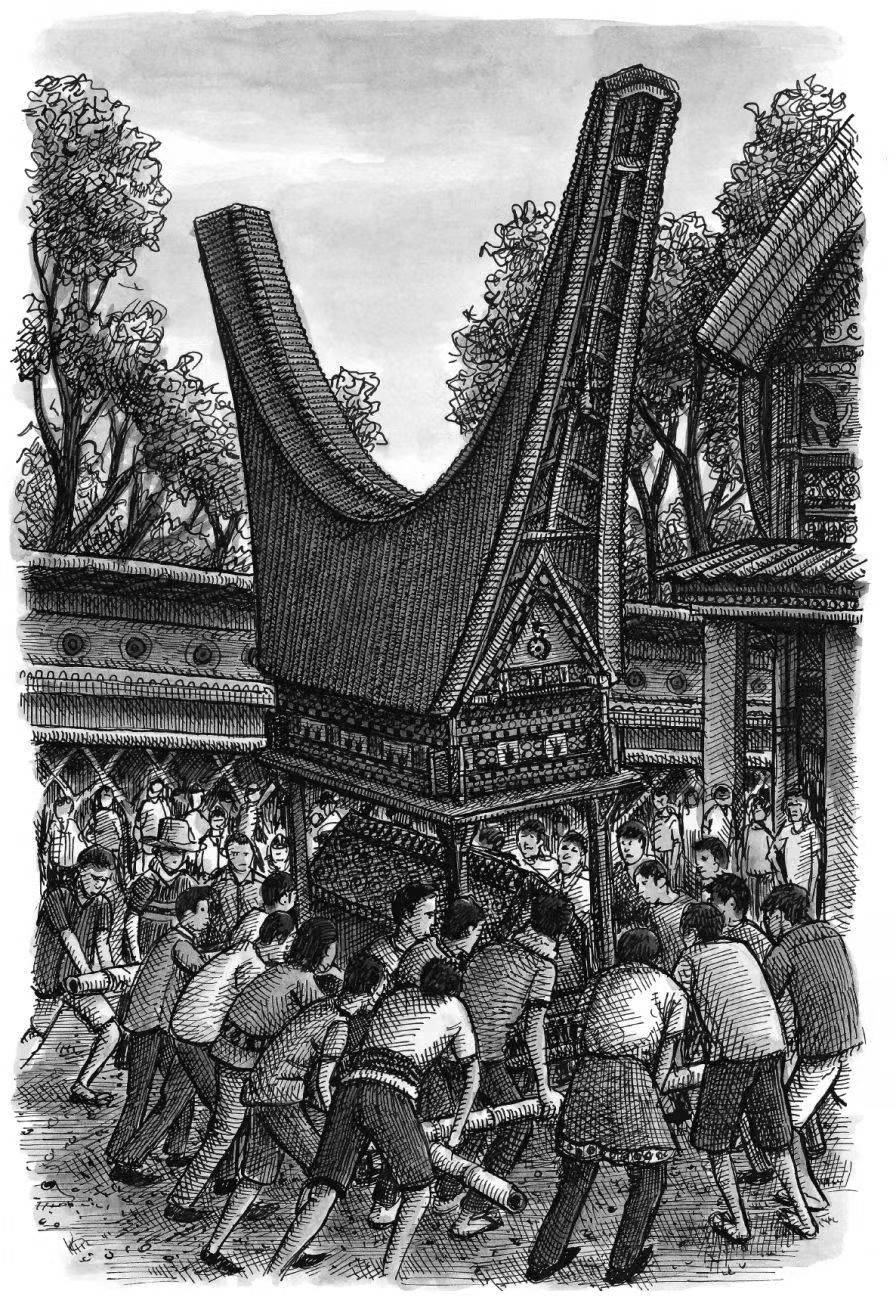
\includegraphics[width=\linewidth ,totalheight=0.95\textheight , keepaspectratio]{塔纳托拉雅的葬礼.jpg}
\caption{塔纳托拉雅的葬礼}
\label{fig:ta_na_tuo_la_ya_de_zang_li}
\end{figure}

人们一拥而入进了院子中央,而抬棺的队伍此时还在外面缓慢前进着。棺房比想象的要沉,小伙子们只能每走半分钟就把它放下来休息。

院子中央有一头强壮的水牛,它神情凝重,仿佛已经猜测到了自己的结局。它被一根短绳子拴在旁边的木桩上,可怜的模样...

游客(我猜的,他们有几个人皮肤白皙,带着西欧口音)统一集中在院子远处的角落里,所在之处和主场地隔着一排栅栏。这个措施反映出塔纳托拉雅死亡旅游业的一个棘手问题:如何才能既让游客近距离参观,又不让他们离得太近。我们也在这个“看台后排区”,但我不觉得有什么不妥。我找好地方坐下,保罗拿出相机准备拍照。为了让自己在闷热潮湿的天气里好过点儿,保罗今天换了一身行头:一件牛仔上衣、一条牛仔工装裤、一个警长徽章、一双波点短袜和一顶牛仔帽。

有些游客不太明白“后排区”的意义。一对夫妇直接坐进了留给死者家属的贵宾区。但当地人太客气了,没好意思把他们赶走。一个染着扎眼金发的德国老太太径直走到院子中央,用iPad对着小孩的脸就是一顿猛拍,还一支接一支地抽着红色万宝路烟。我真想找根拐杖钩着她的脖子把她弄走。

塔纳托拉雅的旅游业在最近几十年才兴起,20世纪70年代之前几乎没有人听说过这个地方。当时,印度尼西亚政府重点开发巴厘岛和爪哇岛的旅游业(事实证明他们做得很成功),忽视了塔纳托拉雅的独到之处——观赏性和仪式性兼具的传统葬礼。塔纳托拉雅不想再被其他印度尼西亚人看作“割取别人首级进行黑巫术”的地方,而是希望以保存良好的传统文化而闻名。

遗体终于被抬进了院子。抬棺人将棺房举起再放下,如此反复,口中哼着歌谣。他们一刻不停,直到全身的力气用尽之后才把棺房放到地上。他们喘了几口粗气,接着又把棺房扛在肩上,重复之前的动作。这种力量的交替让我看得入迷,西式葬礼的抬棺仪式一下子就显得有些古板。

这具遗体生前属于罗文纳斯·林汀。他是一位政府公职人员,也是一个农民,是村里的重要人物。我身后就放着一张5英尺高的照片,上面是林汀先生的脸部特写。照片里的人大概60岁,留着细长胡须,穿着时髦的蓝色西装。

身穿特色串珠服饰的小孩子在院子里追逐打闹,不时给搬运活猪的人让路。这些猪绑在竹板上,不断地发出尖锐的叫声。几个人把猪抬到屋后宾客看不见的地方。主屋的大门前挂着一个门帘,上面画满了迪士尼公主。在贝儿公主、爱丽儿公主和爱洛公主的注视下,这些猪穿过了通向屠宰场的大门。不知道我们早些时候碰见的黑毛猪是否也在其中。

塔纳托拉雅的葬礼可不是普通的自带酒水型(这里的“水”是水牛的“水”)活动。每一只献祭的动物都来自不同的人家,而且有记录可查。因为这套份子体系,人们通常不会错过别人的葬礼。就像阿古斯说的:“你在我妈妈的葬礼上送来一头猪,那我也要在你家举行葬礼时还一头。”看来,塔纳托拉雅式葬礼和美国葬礼一样,也存在过度花费的问题,因为不愿意被人看作不尊重死者。

到目前为止,这场葬礼上的仪式看上去都很繁复\footnote{繁多复杂。},但阿古斯说这已经比从前简单多了。阿古斯的父母从出生起就信奉阿鲁克教,但父亲在16岁时皈依了天主教。对此,阿古斯的解释是:“阿鲁克教里有7777种仪式,这太复杂了,人们只好改信别的。”我可不觉得天主教的仪式少,但就这样吧。

当牧师走到麦克风前开始布道时,人们安静下来。我听不懂他在讲什么,但能听出有几次他停下来,大声呼喊死者的名字向其致意:“罗——文纳斯,林——汀——!”他连续不停地讲了20多分钟,内容大多是重复的。很多人都准备离场,这时他贴近麦克风大吼了一声:“CO——E——!”那个动静活像是死亡金属乐队的主唱发出来的。告诉你,如果你恰好坐在音箱边上,却没在“CO——E——!”这个词出现时及时逃开,后果一定惨不忍睹。阿古斯告诉我,“COE”类似“好好听着”。据说,塔纳托拉雅的葬礼悼词在近几年深受电视节目的影响(舞蹈风格和服装设计也是)。

按照西方医学对死亡的定义,罗文纳斯于5月底去世,也就是葬礼前3个月。但按照塔纳托拉雅的习俗,他其实还活着。虽然已经没有了呼吸,但塔纳托拉雅人认为他只是处于类似发烧这样的生病状态。这个状态会一直持续到人们献上第一个活祭,通常是一头水牛或一头猪。献祭之后,罗文纳斯就可以ma’karu’dusan(咽下最后一口气),和作为祭品的动物一起死去。

人类学家迪米特里·辛吉罗尼斯在塔纳托拉雅进行了两年的田野研究,其间和一位名叫奈拉雅的当地老人建立了深厚的友谊,老人把迪米特里看作亲儿子一般。9年之后,迪米特里重返塔纳托拉雅,本以为能给奈拉雅一个惊喜,没想到她已经在两周前去世了。迪米特里来到奈拉雅家,她的一个亲戚把他领到后屋,然后告诉奈拉雅,迪米特里“回来了”。

\begin{quotation}
我端详着她的脸,然后盘腿坐下,在她耳边轻声问好。虽然一侧脸有腐烂、脱落的迹象,但她看上去十分宁静、安详……她只是“睡着”(mamma’)了,但她“知道”(natandai)我来看她了。不仅如此,她听得到也看得见我。她没有“死”(mate),只是“生病”(hot)了。因此,她还是“能够感受到一切”(nasa’dinganapa-apa)。
\end{quotation}

按照塔纳托拉雅的习俗,遗体在葬礼之前要放在家中。这听上去好像没那么震撼,但让我告诉你,在家中这段时间少则几个月,多则好几年。在此期间,死者的家人负责把遗体制成木乃伊,还要给他送饭、换洗衣物,时不时还要跟他说说话。

保罗第一次来塔纳托拉雅时,问阿古斯是否觉得家里待着一个已经死掉的亲戚很恐怖。阿古斯听了后放声大笑:“我小时候,我爷爷的遗体在我家待了7年。我跟我哥哥,我俩和他睡在同一张床上。每天早上,我们都给爷爷穿好衣服,然后把他靠墙立着,晚上睡觉时再把他放回床上。”

根据自己的所见所闻,保罗认为在塔纳托拉雅,死亡并不是一道强行把生者和死者隔开的“难以逾越的鸿沟”,而是一个模糊的界限。塔纳托拉雅人万物有灵的信仰也强调人类和非人类,不管是动物、高山还是尸体,两者之间都没有绝对的隔阂。

牧师总算讲完了,最后一嗓子“好好听着”也逐渐从音箱中消失。保罗轻轻走到我身边,低声说:“他们杀死那头牛后,应该顺手把某些游客也解决了。”

这时,两名男子好像收到信号一般,同时向院子里的水牛走去。一个人把一根蓝色的绳子从牛的鼻环中穿过。他的动作很轻柔,一边操作,一边用手挠着牛的下巴。水牛貌似没有意识到自己成了全场的焦点。另一个人蹲下来,把它的两只前蹄拴在地上的木桩上。

我不确定自己还在等待什么,也许是一段吟唱,也许是死者家属的相聚?这时,第一个人牵起牛头,从腰带里抽出一把砍刀瞬间割开了牛的喉咙,整个过程只有几秒钟。水牛向后仰起身躯,健壮的肌肉和牛角清晰可见。它想逃跑,却被绳子牢牢地固定在原地。一道鲜红的刀口出现在它的喉咙上,但没有血流出来,看来刀口不深。

好几个人冲上前拽住牛鼻环上的绳子,但没能制服它。水牛又踢又踹,猛烈地摆动自己的身躯,喉咙上的伤口撕裂开来,暴露在众人面前,这个场面让人难以直视。一个人拿出砍刀,朝牛脖子再次砍了下去。这一次,鲜血瞬间喷溅出来。

水牛发疯似的腾空跳起,力量大到挣脱了绳子和木桩的束缚,跌跌撞撞地冲向右侧的人群。现场一片混乱,尖叫声此起彼伏。我用小型摄像机拍下的视频记录下来的全是沉重的呼吸声和踩踏地面的闷响。我周围挤满了慌张的人,推搡之中,我不小心割破了手。

当时,我确信会有人(很可能是我自己)死于水牛的报复行动。最后,司仪成功把牛抓回了院子中央。不久之后,水牛倒地死去,喉咙上的伤口汩汩地往外冒着血。人群中有人哭有人笑,两种截然不同的声音混合成一种缤纷的复调。刚才的惊心动魄向葬礼注入了一丝活力。

\begin{center}
* * *
\end{center}

阿古斯正在打电话,语气很激动。

“出什么事儿了?”我问保罗。

“我们得带头猪过去。”

“我们去哪儿找猪啊?”

“阿古斯说他可以帮忙。不带头猪过去不礼貌。”

阿古斯的车已经坐满了,里面有我、保罗、阿古斯、司机和阿托——一个搭顺风车去隔壁村庄的15岁少年。车上已经没地方放猪了。

阿古斯挂断电话,向我们宣布道:“明天,我的一个朋友会骑摩托车把猪送来。”

阿托一路上都在疯狂地发短信。和一群成年人挤在一辆车里,换作哪个青少年都会这样吧。阿托家将在马聂聂节上给他叔叔和曾祖父开棺,这两个人在阿托还没出生的时候就去世了,因此阿托只能和他们的遗体相逢。

我们到达了目的地。这是一个由多个独立小村庄组成的村镇,没有所谓的中心。大部分村民都以种植水稻为生,包括我们此行的东道主。他们几户人家住在传统的长屋里,一共七栋,中间是公共生活用的庭院。院子里,一群红冠大公鸡正被几只瘦骨嶙峋的狗追着跑,边跑边“喔喔”地叫,狗后面还跟着几个笑哈哈的小孩。女人们正在用细长的竹竿敲打刚收获的稻谷,动作一刻不停。

村子里陆陆续续来了不少人,他们开始帮忙清理房子状的墓室。村子现在共有十几个墓室,都在自家屋子附近。每个墓室的门上都挂着一把大锁,这在以前是没有的。这么做不是为了提防邻居,而是因为几年前有人从村里偷走一具干尸,卖给了兰特包的一个收藏家。后来,村民打听到了是哪个收藏家,又去人家那里把干尸偷了回来。

几个人正聚在一起讨论如何给墓室通风。两年前,村里安葬了一个名叫约翰·汉斯·塔皮的村民。现在,他的深色木质棺材翘开了一个角,一打开墓室的大门就能看见。塔皮的儿子担心墓室里的空气过于潮湿:“希望父亲没什么事。但愿他还是干燥的,没有腐烂。”

今年的马聂聂节对约翰·汉斯·塔皮可谓意义重大。他的儿子认为,父亲在两年前去世时,家里在物质方面做得不够好——当时家里穷,没有杀牛献祭。他对此一直耿耿于怀,坚信没有活祭的话,“父亲就不能转世再生了”。不过,这一切将在这周改变:献祭的水牛已经选好了,正拴在附近的空地上呢。

两个墓室已经打扫完毕。一个女人敞开墓室的门,拿着一大罐柠檬味清新剂往里喷。

路的尽头有一户人家刚刚宰完猪,正等着新教牧师前来给他们新建的、能装下六个家庭成员的墓室赐福。他们邀请我们共进晚餐。

切成块的猪肉盛放在竹盘里,正架在火上烧烤。猪是在炉子旁边杀掉的,现在我们就坐在干掉的猪血旁吃晚饭,几只苍蝇绕着我们飞来飞去。不远处的竹架上挂着几只猪蹄。一只小狗冲进来,叼起一块滴着血的猪下水\footnote{猪下水,也叫猪下货、猪杂、猪杂碎,一般指猪内脏,或部分其他器官。}就往外跑。“哎哟!”厨子冲小狗大叫了一声,但没有阻止它带走战利品。

一个女人递给我一片竹叶,上面放了一个热乎的粉色饭团。这时,有人把竹盘上的肉从火上取下来,一大堆肥肉烧得滋滋作响。吃到一半时,我把这盘肉拿到跟前仔细瞧了瞧:焦脆的脂肪表皮上,一个个毛囊清晰可见。这可是动物尸体上的一块肉啊,我突然反应过来,随即感到一阵厌恶。

我虽然在人类遗体上花了很多时间,但不熟悉动物尸体,不是包装在保鲜膜和塑料泡沫盒里的动物我就不认识。法国人类学家努艾莉·维亚莱斯的一篇关于法国食物体系的文章中有一段话,我觉得也适用于西方其他国家:“屠宰被认为应该是工业化的,即大型化、统一化。不能存在暴力(最好是无痛的),也不能被人看见(最好根本不存在)。这几点即使做不到也要做到。”

\begin{quote}
即使做不到也要做到。
\end{quote}

饭桌上有一位老奶奶,年龄大到眼睛里蒙上了一层白膜。她拿起一小撮米饭,看向屋外山谷的方向。她不怎么与坐在旁边的人交流,也许她已经说不动话了。阿古斯用沾满猪肉残渍的手指捅了我一下,然后悄声说道:“那个新墓穴应该就是给她准备的。”阿古斯在调侃她,但说的也算是事实。这位老奶奶很快就会踏上祖先走过的路,搬到她的新房子里,那个“没有火也没有炊烟的房子”。

夜里,我们的猪乘着摩托车到了。它一着地就钻进其中一栋木屋,狼吞虎咽地吃着泔水。它完全没有意识到,因为我和保罗,这里将成为它的葬身之地。

这天晚上,我们都住在长屋里。长屋从外面看上去很宽敞,但我们进屋爬上梯子后却惊讶地发现,楼上只有一个没窗户的单人间。好在房间的地板上已经铺好了被褥,我们躺下后很快就睡着了。后半夜时,我们才意识到这里不是单人间,墙壁上的木闩拆下后,推开就可以看到另外三间屋子。一整晚都有人蹑手蹑脚地在我们房间周围进进出出。

\begin{center}
* * *
\end{center}

第二天一早,一阵阵凄凉的铜锣声从路边传来,正式宣告马聂聂节拉开帷幕。

我见到的第一具木乃伊戴了一副20世纪80年代的飞行员墨镜,镜框还镶着金边。

“哎哟,”我心想,“这哥们儿跟我中学的代数老师一个风格。”

一个年轻人把这具干尸立起来,另一个人拿起剪刀,把他身上的蓝色上衣从领口一路向下剪开,直到露出内裤边缘。木乃伊的上身和双臂就这样暴露在空气中。这个人虽然已经死去八年,但遗体保存得非常完好,表面上没有肉眼可见的伤口或裂痕。跟他隔着两具棺材的哥们儿就没那么走运了:全身上下都皱巴巴的,只有一层薄薄的干皮勉强搭在骨头上,要不是裹了一条镶有金边的毯子,估计早就散架了。

刚才那具木乃伊被放在地上,头下垫了个枕头,身上只剩下平角短裤和飞行员墨镜。一张8英寸×10英寸的遗像照片摆在它身旁。照片上的他看上去一点儿也不像我的代数老师,人在八年间的变化还真大。

几个女人在他旁边跪下,一边轻抚他的脸颊,一边大声哭着呼唤他的名字。当哭喊声逐渐停下时,他的儿子手捧一套工具刷(就是五金店里卖的那种)走了过来,开始清洁遗体。他用刷子轻轻扫过父亲粗糙的皮肤,每一下都很利落,并且充满爱意。一只蟑螂从父亲的平角短裤里蹿了出来,但他好像并不在意,继续手里的动作。这种打理遗体的方式我还是第一次见。

10分钟前,阿古斯接到一个电话,对方说有一家人正在河边一处难以到达的墓室中给死者开棺。我们迅速沿着水稻田旁的土路朝那个方向跑去。路的尽头是一条棕黄色的泥沟,附近没有垫脚的石头,也没有桥。我们只好一边抱怨,一边从泥里蹚过去,其间我还摔了个屁股蹲儿。

到达目的地后,我们看到至少有40具遗体被抬了出来,在地上一字排开。有些遗体裹着颜色鲜艳的布料,有的放在狭长的木质棺材里,还有的用印满卡通图案——凯蒂猫、海绵宝宝,以及一大堆迪士尼卡通人物——的毯子包着。这家人在遗体间走来走去,商议要先给谁开棺。有些死者他们已经不记得是谁了,有的则是重点关照的对象,比如某人亲爱的丈夫或某家的宝贝女儿,他们的家人都迫不及待地想再见到他们。

一个母亲正在打开16岁儿子的棺材。最先露出来的是一双弯曲变形的小脚,然后是手,看上去保存良好。站在棺材两侧的人试着抬起男孩,他们动作轻柔,确保不会碰坏遗体。他们成功地把男孩立了起来。男孩的躯干完好无损,但头部已经白骨化了:牙齿清晰可见,浓密的黑发还连在头皮上。但他的母亲毫不介意,此刻正欣喜若狂地看着他。这份喜悦也许是一时的,也许她从来都是这样,但不管如何,现在她正握住他的手,轻抚着他的面庞。

附近有一个人在用刷子清洁父亲的遗体。父亲的脸被蜡染布料制成的裹尸布染成了粉红色。“他是个好人,”他说道,“他有八个儿女,但他从没打过我们。我很难过,但又很开心,因为我现在能照顾他了,就像他以前照顾我那样。”

塔纳托拉雅人会把自己接下来的动作讲给遗体听:“现在,我要把你从坟墓里移出来。”“抱歉只给你买了烟,我最近手头有点儿紧。”“现在,我要脱掉你的外衣。”“你女儿和女婿从望加锡过来看你了。”
我们在这个河边墓穴碰到了这家的族长,他对我们的到来和送上的香烟表示感谢。他允许保罗拍照,也同意我问问题,但条件是答应他的一个请求:“如果你们在村子里碰见外来人,不要告诉他们这个地方,这里是我们的秘密。”

我想起前几天葬礼上那个粗鲁的德国女人,一边抽烟,一边把iPad贴在别人脸上乱拍。我担心自己也变得跟她一样——我们渴望把期待已久的事物看个遍,但不承想这让我们变成了不受欢迎的人。

\begin{center}
* * *
\end{center}

我们穿过稻田返回主路,正好赶上东道主开棺打理自己家的遗体。我认出一个在兰特包当平面设计师的同龄人。昨天深夜,他骑摩托车赶了回来,在我们睡觉的房间钻进钻出。他指着一具包在金色布料里的骷髅说道:“这是我兄弟,17岁时骑摩托车出车祸死了。”然后指了指旁边的遗体,“那是我爷爷。”

我们下方的山坡上有一家人在野餐。用餐完毕后,他们把死去七年的祖父平放在方格桌布上。这是他祖父第二次参加马聂聂节,遗体状态极佳,看不出有任何损坏。这家人先用软刷清洁他的面部,再把他翻过来清理脑后干裂开的皮肉。拍摄全家福时,祖父被立在中间,家庭成员纷纷围过来,有的表情严肃,有的面带笑容。我正津津有味地看着,一个女人招呼我过去一起合影。我朝她摆摆手,意思是“还是不用了吧”,但他们坚持要叫上我。于是,一张奇特的合影出现在印度尼西亚的深山里,上面是我、一个塔纳托拉雅家庭和一具焕然一新的干尸。

我之前听说把遗体制成木乃伊通常发生在气候寒冷干燥的地区,没想到在湿润多雨的印度尼西亚也能这么做。那么问题来了:这里的遗体究竟是怎么变成干尸的呢?不同的人会给你不同的答案。有人说他们用的是自古流传下来的方法——把油灌入死者的嘴巴和喉咙里,再用特制的茶叶和树皮覆盖全身。茶叶的茶多酚和树皮将皮肤中的蛋白质收紧,从而强化了皮肤的柔韧性和硬度,这样就能够更有效地抵挡细菌入侵。这个过程与标本师对兽皮进行处理使之长久保存的过程类似(所以有一种皮革叫“植鞣皮”)。

塔纳托拉雅现在还流行一种新潮的干尸制作方式:把防腐师的好朋友福尔马林注射到遗体中。有一个女人告诉我她无法接受这种方式,因为不愿意死去的家人被针扎。“但我知道有人这么做。”她压低声音说,好像发现了什么见不得人的事。

生活在塔纳托拉雅这部分的村民可以称得上业余人体标本师了。既然他们现在和北美人民都用同一种化学制剂给尸体防腐,我不明白为什么西方人依然会被他们的习俗吓个半死。原因应该和尸体干燥的程度无关,而在于塔纳托拉雅人不把遗体密封在棺材里,也不把棺材搁置在水泥做成的地下墓穴里,而是大大方方地让遗体和活人待在一起。

昨天,我碰到了约翰·汉斯·塔皮的儿子,今天我要去见约翰·汉斯·塔皮本人。他被平放在地上晒太阳,身上只穿了一条平角裤,手腕上戴了一块金表。他的胸腔和腹腔注满了福尔马林,因此这两处保存得异常完好。相比之下,他的面孔已经变成黑色,上面布满了斑点,白色的骨骼依稀可见。这时,他的家人把刷子伸到他的平角裤里,开始清洁他那干瘪的阴茎。不出意料,家人的脸上写满了尴尬。他们互相开了个玩笑,然后继续手里的活儿。

小孩子们在木乃伊之间跑来跑去,他们有时会在某具遗体面前突然停下,仔细瞧一瞧之后再伸手捅一下,然后大叫着跑开。一个5岁的女孩爬了上来,和我一起坐在一个墓室的屋顶上看着他们玩闹。我俩没有说话,心照不宣地享受着俯视他人的奇妙快感。

阿古斯发现我在屋顶上,向我喊道:“喂,我在想我之后是不是也会变成这样。肯定会的,是吧?”

我们回到留宿的那栋房屋后,一个4岁的男孩过来偷看我们吃饭。他从篱笆后面探出头,每次我回头冲他做鬼脸时,他都开心地大叫。这时,他妈妈过来告诉他不要打扰我们,于是他给自己找了个小刷子。他穿过院子走到一堆干竹叶旁坐下,用刷子全神贯注地在地上刷来刷去,保证每一条小裂缝都被刷到。如果马聂聂节一直存在,长大成人的他也一定会去清洁某具遗体,遗体的主人说不定就是我们这次碰见的某个村里人。

\begin{center}
* * *
\end{center}

第二天清晨,约翰·汉斯·塔皮已经换上了一套新衣服...。他今天要被搬去路尽头的一间新墓室里,墓室的墙壁是浅蓝色的,屋顶上立着一个白色十字架。里面的装饰走的是多元文化路线:除了传统的水牛符号之外,还有玛利亚之心、耶稣祈祷像以及《最后的晚餐》全景图。

家里人把约翰立起来,跟穿着新衣的他拍了最后一张合影,便把他放回棺材。他们把闪亮的黑皮鞋从他脚上脱下放在旁边,给他裹好毯子,随后合上了棺材盖。棺材两侧被擦拭干净之后,他们就把棺材扛在肩上出发了。鼓声和诵经的声音伴随了他们一路。

我往车上装东西时,阿古斯走了过来。“知道吗,现在就有具尸体在这栋房子里。”他指着跟我们木屋只隔了10英尺的一栋传统房屋说道。一位名叫山达的70岁老太太两周前死在这栋房子里。这家人一直瞒着我们,就是想看看我们知道后会有什么反应。

“你想见见她吗?”阿古斯问道。

我慢慢地点了点头。不知为什么,我觉得我们应该就睡在尸体隔壁。

“嘿,保罗,”我叫醒正在屋里补觉的保罗,“跟我下楼,给你看样东西。”

在阿古斯的指导下,我们给山达带来了一些吃剩的食物——她应该知道是我们送的。我们钻进里屋,看到山达躺在一张竹席上,身上盖着一条绿色的格纹毯子。她穿着一件橘色的衬衫,脖子上围了一条粉色的围巾,身边还放着钱包和食物。她的脸上围着一块布,面部皮肤有着橡胶般的质感,这在防腐后的遗体上很常见。

山达是由一个本地的专业人员用福尔马林防腐的。她的家人没有亲自操作,因为觉得福尔马林太“辣眼睛”。山达一家子都是成功的稻农,没有时间按照传统天天照料她的遗体。

她会在家里一直住到搬进墓室。这期间,家人给她端茶倒水,她在梦里与家人相会。距离她穿过生与死那条模糊的界限只有两周,因此家里人决定,等味道散去后就跟她一起睡。

阿古斯小时候跟他祖父的遗体睡了七年。他耸了耸肩,说道:“这种事情我们已经习惯了,这就是生与死。”

\begin{center}
* * *
\end{center}

在前往印度尼西亚之前,我试图在网上查询与塔纳托拉雅有关的信息,想先看看会有什么样的丧葬仪式在等着我。搜索出来的信息很少,起码没什么英语的。

照片也没有几张,其中最清晰的一张来自英国报纸《每日邮报》。我不知道他们是从哪儿得到的这张照片,因为他们显然没有派记者去。页面上的评论区很有意思,一条评论写道:“天哪,他们对这些逝者做了些什么呀?”另一条评论则写着:“讲真,这是对死者的大不敬。”

确实,如果说把莎莉姨妈从明尼苏达的坟里挖出来,把她放到高尔夫球车上在郊区民宅附近转一圈儿,那么是的,这的确是对死者的大不敬。但这些心智不健全的网友没有意识到,人死后,亲情还会继续存在。塔纳托拉雅人不但不觉得开棺掘尸是对死者的不尊重(事实上,这是对死者最大的尊重),而且认为这是与逝去的家人维持情感的一种方式。

作为一名殡仪业者,我总会碰到各种各样关于母亲遗体的问题。你不知道我听到了多少次:“我妈妈11年前在纽约州北部去世,防腐后葬在我们的家庭墓地里,你能告诉我她现在变成什么样了吗?”这个问题的答案取决于多个因素:天气、土壤、棺材、化学品。所以,我给不出一个完美答案。当我看到塔纳托拉雅人与母亲的遗体互动时,我意识到他们不需要通过殡仪人员了解遗体的状况。他们很清楚自己的母亲死后是什么样子,哪怕她已经死了11年。相较于与死去的母亲重逢,还是人类的胡思乱想更可怕一些。


\end{bookref}

\section{墨西哥的米却肯州}
\begin{bookref}[frametitle={\cite{好好告别}}]
一具头戴黑色圆顶高帽、嘴里叼着雪茄的骷髅疯狂地挥舞着细长的双臂,朝华雷斯大街俯冲下来。这个庞然大物高达15英尺,在黑压压的人群中显得极为壮观。一群打扮成卡特里娜骷髅的男人和女人跟在它身后,一边欢呼雀跃,一边舞蹈。华丽优雅的卡特里娜骷髅是这里的标志性形象。当身着阿兹特克勇士戏服的旱冰方阵表演旋转时,一大片金色亮片从礼花炮中射出,街上的几万名观众顿时爆发出热烈的欢呼。

如果你看过2016年的詹姆斯·邦德电影《007:幽灵党》,就会认出这充满了鲜花、骷髅、魔鬼和大型卡通气球的狂欢,正是墨西哥城一年一度的亡灵节大游行。这部电影的片头,就是西装革履的邦德戴着骷髅面具穿过嘈杂的人群,与一名同样戴着面具的女子溜进了旅馆。

不过请注意,这部邦德电影并没有从亡灵节大游行中获取灵感,亡灵节大游行反倒是因为这部电影才存在的。墨西哥政府担心世界各地的人们观看完影片之后,会来墨西哥参加其实并不存在的游行,于是现招募了1200名志愿者,用一年的时间打造出这场四个小时的盛会。

亡灵节为每年11月的头两天。在这两天里,死去的人会重返人间,与活人一同享受人间的乐趣。在有些人看来,这个愚蠢的游行把本应以家庭为中心的、私人化的节日庆祝商业化了。另外一些人认为,这恰好代表了亡灵节正在向更加世俗的全国性节日演变,在全球的瞩目下毫不畏惧地展现墨西哥的历史文化。

游行结束后,我们艰难地走在装饰亮片成堆的街道上。跟我同行的是莎拉·查维斯,她是我建立的非营利组织“死亡新秩序”的总监。她发现这里到处都有亡灵节的装饰品,不管是在家里还是在商店,卡特里娜骷髅和鲜艳的骷髅剪纸随处可见。

“噢!”听起来她好像突然想起一件重要的事,“忘了告诉你,我们酒店旁边的星巴克在卖亡灵面包。”亡灵面包就是一种撒满糖霜的、带有立体骷髅造型元素的圆面包。

明天,我们就要动身前往西部的米却肯州。那是比较偏远的地区,当地人有着漫长的庆祝亡灵节的传统。但是在墨西哥,亡灵节在20世纪的一段时间里并没有受到普遍欢迎。到了20世纪50年代,墨西哥的城镇居民仍然把亡灵节视作老掉牙的民俗节日,认为只有文明社会里的边缘人才会庆祝这种节日。

这种情况不久之后就迎来了反转,主要原因之一就是万圣节从美国南部传入了墨西哥。在20世纪70年代早期,用记者玛利亚·路易莎·门多萨在她的文章中的话来说,万圣节习俗的核心就是“光彩夺目的聚会”。“黑猫、南瓜和戴着尖顶帽坐在扫帚上的女巫如果只是出现在侦探小说里,我倒觉得还好,因为这些东西跟我们的文化一点儿关系都没有。”门多萨继续写着,“普通的墨西哥人忽视了那些乞讨要饭、靠擦车窗讨生活的孩子。在富人区,我们的中产阶级模仿美国得州人,让孩子们穿上可笑的服装去别人家里要施舍。要知道,这些孩子从未空手而归。”

学者克劳迪奥·龙尼茨对这一时期是这样描述的:亡灵节“变成了国家形象的统一代表”,站在了“美式万圣节狂欢”的“对立面”。那些曾经抗拒亡灵节(或者生活在从不庆祝亡灵节的地区)的人逐渐把庆祝亡灵节视作墨西哥的传统。亡灵节不仅回归了主流城市(瞧瞧那个邦德引发的大型游行),还成为丧失权利的弱势群体的发声通道。他们在亡灵节上悼念那些远离公众视野的人,包括性工作者、本土性少数人权倡议团体和死在美墨边境线上的同胞。在过去的40年间,亡灵节成为整个墨西哥的流行文化、旅游文化和反抗文化的代名词。墨西哥本身也因成功地打造了全民参与的祭奠文化而走在世界前列。

“我小时候,跟我一起生活的长辈都是一些自我厌恶的墨西哥人。”莎拉说道,此时我们正坐在米乔坎的酒店房间里,“他们生活的环境告诉他们,他们没什么可自豪的,他们应该对自己的一切感到羞愧。他们应该融入。要想在美国获得快乐,就得变得和白人一样。”

20世纪初期,莎拉的祖父母从墨西哥蒙特雷搬到东洛杉矶的查维斯山谷区定居。20世纪50年代,政府通过公函告知该地区的近2000个家庭——大多都是低收入的墨西哥裔美国农民——他们必须卖掉自己的房产,给政府的公共住房项目腾地方。政府保证,在项目完成后,不仅会在原地新建学校和操场,还会优先给予搬迁居民回迁的机会。这些家庭只好搬走,原先的社区也被拆毁。然而,洛杉矶政府取消了公共住房项目,转而与纽约的商人共同兴建道奇体育场。包括罗纳德·威尔逊·里根在内的体育场项目支持者公然把反对者称为“痛恨棒球的家伙”。

由于一项歧视性的住房政策,从查维斯山谷区搬离的墨西哥裔美国人被赶到洛杉矶东部。在搬迁的过程中,莎拉的父母步入成年,二人在19岁的时候生下了她。

“直到今天,我的奶奶、姑姑和叔伯一谈到查维斯山谷区,还是会伤心得不得了。他们特别、特别想念那个地方。”

莎拉出生后,她的家人不允许她学西班牙语。她的浅色肌肤让她成为家里最受宠爱的孙辈。她墨西哥人的一面只能留在家里。在洛杉矶长大的莎拉,不停地游走在与她关系疏远的母亲、在好莱坞从事服装道具营生的父亲(时至今日,他都认为自己是“美国原住民”,而不是墨西哥人)和祖父母之间。莎拉只当自己是个碰巧带有墨西哥血统的美国人,家里的墨西哥文化氛围和自己的关系不大。

2013年,莎拉已经在学前班和幼儿园当了10年的老师。她与自己工作上的搭档鲁本坠入爱河,不久后,两个人决定是时候要个孩子了。莎拉很快就怀孕了。对她来说,有了这个孩子就意味着“一个真正的家庭,我的家庭,一个天选之家,没有谁能从我手里夺走”。

可惜事与愿违,莎拉的儿子在六个月大的时候胎死腹中。在接下来的日子里,莎拉心里“放不下任何人、任何事”。她与父母渐行渐远,觉得自己孤独极了。有那么几天,她甚至想消失在房屋后面的橙树林里。她不停地自责:是不是我搬东西的姿势不正确?我是不是吃了不该吃的东西?“女人的本质是带来生命之人,”莎拉说道,“我的身体却是一个坟墓。”

她觉得对朋友和同事来说,自己就是一个行走的辐射源。她知道,在人们理想中的世界里,孩子是可爱的,不会受到伤害。“这个社会要求我藏起悲伤,”她继续说道,“人们不想面对这种恐惧,而我恰好就成了这种恐惧的代言人。我是一个恶魔。”

莎拉在网上搜遍了那些遭受丧子之痛的母亲的故事。她找到了几个好心人建立的网站,但它们都带有一些基督教的意味(例如,“我的天使躺在上帝的臂弯中”),里面的故事也是老生常谈,一直在绕弯子。在她看来,这些看上去很美的话不过是一堆空洞的陈词滥调,无法捕捉到她的悲痛和渴望。

在寻找安慰的过程中,她将目光转向了自己的文化与传统。“莎拉,你是墨西哥人,你来自无疑是这个世界上与死亡关系最紧密的文化。”她想,“你的祖先会如何处理这种悲剧呢?”
\begin{center}
* * *
\end{center}
墨西哥诗人奥克塔维奥·帕斯有一段著名言论。他说,当纽约、巴黎、伦敦等西方城市的居民还在担心频繁提起“死亡”这个词会让自己“咬到嘴巴”时,“墨西哥人已经无时无刻不在谈论它、嘲讽它、爱怜它、取悦它,甚至与它同眠。死亡是墨西哥人最喜欢的玩乐之一,也是他们永恒的挚爱”。

不过,这并不意味着墨西哥人不惧怕死亡。他们与死亡的联结源自长达几个世纪的暴行,可谓来之不易。“墨西哥没有成为一个令人骄傲并强大的帝国,”克劳迪奥·龙尼茨解释道,“这个国家不断被列强和独裁者欺压、侵略、占领、分裂、敲诈。到了20世纪,当西方世界对墨西哥的镇压和对死亡的抗拒双双达到顶峰时,墨西哥与死亡之间愉快、亲密的联系逐渐成为国家形象的奠基石。”

对莎拉而言,接受儿子的死不等于抹杀对死亡的恐惧,她知道自己不可能不惧怕这必然的命运。她只是想适应死亡,只是想开诚布公地谈论死亡。就像帕斯说的,时刻“谈论它、嘲讽它、爱怜它”。

许多来自移民家庭的孩子发现自己越发远离家族所传承的文化传统,就像莎拉经历的那样。臭名昭著的美国殡葬体系通过立法和出台管理条例,大肆干预多元化的丧葬习俗并强制其与美式规范同化。

莎拉最初是通过画家弗里达·卡罗的作品与墨西哥文化建立起联系的。弗里达·卡罗是墨西哥的“痛苦的女主人”,对莎拉的影响最为深远。在1932年的画作《墨西哥和美国边境线上的自画像》中,卡罗站在假想出的墨西哥和底特律的边境上,脸上充满了蔑视。那时,她和作为壁画画家的丈夫迭戈·里维拉正在底特律生活。边境线上的墨西哥一侧画满了骨头、废墟、植物、花朵和深深植入土壤中的粗壮的根茎,底特律一侧则是工厂、摩天大楼和滚滚浓烟——一个掩盖了大自然生死循环的工业城市。

在底特律生活时,卡罗怀孕了。她把这个消息写信告诉给了自己的前任医师利奥·埃劳塞,他们二人在1932年到1951年一直密切通信。她担心这次怀孕有很大的风险,因为在那次电车事故中,她的部分骨盆粉碎性骨折,子宫也被刺穿。卡罗在信中写道,底特律的医生“给我开了打胎用的奎宁和高浓度蓖麻油”。但这些化学药品没能终止妊娠,医生也拒绝为她进行堕胎手术。卡罗很有可能要冒着生命危险分娩。她请求埃劳塞给那名底特律医生写信:“堕胎是违法的,他应该是害怕做违法的事。但再这样拖下去,恐怕会错过手术的最佳时机。”我们不知道埃劳塞有没有按照卡罗说的做,但两个月之后,她遭遇了严重的流产。

卡罗以这次经历为灵感创作了《底特律的流产》。画里的她赤裸着躺在医院的病床上,鲜血染红了床单。几个物体飘浮在她的周围,分别是男胎(她的儿子)、手术工具以及具有象征意义的蜗牛和兰花,均由红色丝带做成的脐带连在她的肚子上。底特律了无生气的工业建筑构成了天际线,突兀地矗立在画面后方。艺术史学家维克多·萨穆迪奥·泰勒称,除了表达对底特律发自肺腑的憎恶,哀诉发生在自己身上的可怕不幸,“这幅画作是卡罗第一次有意识地画出自己的故事,画出自己最隐秘、最痛苦的内心”。

莎拉一直淹没在“上帝对你早有计划”这种空洞的说辞中,卡罗的画作和书信里的直白表达对她来说无疑是一种安慰。她在卡罗的身上,看到了另一个因为孩子、身体而被迫与命运的无常进行抗争的墨西哥女人。卡罗用画笔展现出这种痛苦和困惑,毫不羞耻地描绘自己的身体和哀痛。

莎拉的儿子死于2013年7月。同年11月,她和自己的伴侣——同样是墨裔美国人的鲁本在亡灵节时来到墨西哥。“我们不是游客,不是来看‘死亡’的。”莎拉说道,“我们每天都与死亡在一起。”

穿行在精致的祭坛和骷髅装饰品之间,莎拉感受到了在加利福尼亚州从未体会过的冲击与平和。“来到墨西哥后,我发现这是一个能让我放下悲伤的地方。这里认可我的悲伤,我不再是那个让别人不舒服的人。我终于可以喘口气了。”

莎拉和鲁本来到了以收藏木乃伊而闻名的瓜纳华托。19世纪末,当地人要给葬在坟场的死者缴一笔“坟墓税”来获得“永久”埋葬的资格。如果死者的家人交不起这笔钱,那么死者的遗体就会被挖出来给刚死的人腾地方。在一次例行的挖掘作业中,工作人员惊讶地发现挖出来的不是白骨,而是一具具“表情狰狞、形状怪异的干尸”。原来,土壤中的化学物质在当地的气候条件下能够天然地将遗体木乃伊化。

瓜纳华托市政府在接下来的60年里,不断地挖出了木乃伊。轻度干尸化的遗体被直接火化,完全呈木乃伊形态的则作为展品收藏在木乃伊博物馆。

20世纪70年代,作家雷·布拉德伯里到访该博物馆,并以陈列在里面的木乃伊为灵感创作了一个故事。他之后写道:“这个博物馆让我的心灵饱受创伤。我害怕极了,只想赶紧逃离墨西哥。我接连做噩梦,梦见自己死后被当作展品,和一屋子被金属丝线固定的干尸关在一起。”

由于这些木乃伊是天然形成的,不是出于防腐的目的刻意而为之,因此他们都大张着嘴巴,手臂和脖子呈扭曲状。人死后,遗体会重新回到“肌肉松弛的状态”,放松的下颌导致嘴巴张开,眼睑失去张力,四肢的关节也变得极度松垮。总之一句话,遗体不会自己使劲,它们不再按照活人的规矩来。瓜纳华托木乃伊的吓人形态不是为了“吓唬”布拉德伯里先生而人为制作的,那只是人死后正常的生理变化现象而已。

这些木乃伊现在还在展出。莎拉一点儿也不觉得它们可怕,她走到一个黑暗的角落,在一个身穿白色连衣裙、躺在天鹅绒垫子上的木乃伊女童跟前停下。“她看上去像一个被光芒围绕的天使,那一刻,我觉得自己可以永远站在那里看着她。”

莎拉默默地流着眼泪,一个女人看到后递给她一张纸巾,然后轻轻地拥抱了她一下。

博物馆里其他的木乃伊儿童也有自己的专属道具,比如拿着权杖和戴着王冠的Angelitos(“小天使”)。在20世纪早期的墨西哥以及其他拉丁美洲国家,人们把死去的婴儿和小孩视作能与上帝沟通的神体,类似于圣徒。这些“小天使”已经不再背负原罪,能够给尚在人间的家人带来恩惠。孩子的教母负责打理遗体,她把遗体清洗干净,然后给遗体穿上小号的圣徒服装,再把蜡烛和鲜花摆在遗体周围。孩子的母亲在这个过程结束之后才能见到遗体。此时,呈现在她眼前的是一个不再带有世间忧伤的天人,已经准备好回到上帝身边了。

孩子的家人会邀请朋友和亲属参加葬礼聚会。这么做不仅是为了缅怀死去的孩子,也是为了给这个孩子留下好印象以获取恩惠——别忘了,这个孩子现在已经拥有了灵力。有时候,人们甚至会带着孩子的遗体参加一个又一个聚会,遗体由同龄的小朋友抬着,后面跟着父母和亲属。“小天使”通常会出现在拥有恢宏场景的照片或画作中。

虽然莎拉不相信圣徒和来世,但是这种文化承认孩童的死亡,这一点深深地打动了她。“他们对待这些孩子的方式太特别了,很多事就是专门为这些孩子做的。”她说道。不管是聚会、作画,还是游戏,这里的人们为死去的孩子做了很多,而不是沉溺在孤独和无尽的缄默中。
\begin{center}
* * *
\end{center}
每年11月1日的夜晚,生与死的界限变得薄弱而模糊,死者轻易就能跨越这道坎儿。在米却肯州的小城圣达菲拉古娜,一群上了年纪的妇女正端着亡灵面包和水果,拜访那些在今年失去亲人的邻居,铺满鹅卵石的小道上到处都是她们走家串户的身影。

我低头钻过画有金盏花的门帘进到玄关。大门正上方挂着一个相框,里面是赫尔海的照片。赫尔海死的时候才26岁。照片上的他反戴一顶棒球帽,身后贴着好几张乐队的海报。“活结乐队?这个我可不好评价,赫尔海。”我琢磨着,同时在思考对一个死人的音乐喜好评头论足是不是不太妥当。“噢噢,那是错配乐队!算你有眼光。”

穿过玄关就是赫尔海的祭坛,一共三层。里面每一个祭品都是他的家人和朋友送来做诱饵的——诱使他在这一晚回家。赫尔海在今年身亡,因此他的家人先在家中设立祭坛,之后再把祭品带去他的坟墓。只要他的家人经常去扫墓,邀请他与生者重逢,他就每年都能回家看看。

祭坛的最下方有一个黑色的高脚杯,里面放着柯巴脂香料,辛辣的气味在空气中飘荡着。水果和面包足足堆了3英尺高,旁边放满了装饰用的蜡烛和金盏花。这一晚,随着越来越多的街坊邻居过来送上自己的那一份祭品,这个祭品台只会变得越来越高。重返人间并不意味着赫尔海要变成一具活跳尸,他会以灵魂的形态回到家中,用灵体特有的方式吃掉那些水果和面包。

摆在祭坛正中间的是赫尔海最爱的白色T恤,上面印着一个表情悲伤的小丑和手写体的“小丑”字样。等待他回家的还有一罐可乐(可乐的魅力我太了解了——这听起来也许有些不着调,但如果家里有一瓶健怡可乐等着我,我也会起死回生的)。T恤的上方挂着一些传统的基督教饰品,我看到了几个圣母玛利亚和一个钉在十字架上的血淋淋的耶稣。天花板上悬挂着色彩缤纷的剪纸,形状是脚踩自行车的骷髅。
祭坛旁边围了十几个人,他们都是赫尔海的家人,正在为迎接客人做准备。他们今晚很有可能要忙活到深夜。几个身穿闪亮公主裙的小家伙跑来跑去,脸上画着卡特里娜骷髅花纹,手里还拿着挖空内瓤的小南瓜,用来装大人给的糖果。

莎拉早就买好了满满一袋糖果。消息不胫而走,一大帮脸上画有骷髅彩绘的小孩提着点了蜡烛的南瓜灯把她团团围住。“女士,女士,谢谢你!”莎拉顺势蹲下,带着幼儿园老师特有的沉着和爱意给他们发糖。“我以前也在亡灵节的时候给班里的小孩做南瓜灯,里面也有蜡烛,跟他们现在手上拿的一模一样。可惜一点儿火光就能让管理部门把活动叫停。”她苦笑了一下。

圣达菲拉古娜是布雷佩查人的故乡,这一原住民以建造造型独特的金字塔和制作用蜂鸟羽毛制成的装饰画而闻名。1525年,布雷佩查人正因天花肆虐而变得脆弱不堪。当听闻勇猛善战的阿兹特克人已成为西班牙人的手下败将时,布雷佩查的领袖只好宣誓效忠西班牙。时至今日,这个区域的学校依旧在实行布雷佩查语和西班牙语双语教学。

许多现在流行的葬礼仪式元素,例如音乐、熏香、花朵和食物,布雷佩查人早在16世纪西班牙入侵之前就使用了。到了西班牙殖民时代,根据一名多米尼加男修士的记载,布雷佩查人很乐意接纳天主教的万圣节和万灵节,因为这跟他们已有的纪念亡者的节日完美契合。

在接下来的几个世纪里,殖民者想方设法地根除原住民祭奠死者的习俗,因为这“吓坏了杰出的精英阶层,他们竭尽全力要把死亡从社会生活中赶走”。1766年,皇家罪案处禁止原住民进行扫墓活动,强行切断了他们与死者的联结。不过,原住民总能找到钻空子的方法,这个习俗也就保留下来了。

我们来到另一户圣达菲拉古娜人家,只见门口的牌子上用布雷佩查语写着“欢迎回家,柯奈李奥神父”。柯奈李奥神父的祭坛占满了一整间屋子。我把橘子和香蕉摞在水果堆的最上方。这时,这个家族里几个年长的妇女围过来,给我们递上一大碗还冒着蒸汽的猪肉炒番茄和几杯玉米粥——一种用玉米、肉桂和巧克力做成的热饮。对死者家属而言,这一晚不能单方面地接受别人送来的慰问品,邻里间的这种交流是相互的,他们也要有所给予。

坐在屋子一角观察我们的正是柯奈李奥神父本人——其实这是一具真人大小的塑像。柯奈李奥神父坐在折叠椅上,身披一件斗篷,脚蹬一双黑色的高帮靴子,头上的白色牛仔帽遮住了半张脸,一副正在睡午觉的样子。

祭坛的中间是一个相框,照片里的柯奈李奥神父也戴着一顶白色牛仔帽,和塑像头上的是同一顶。相框后方的墙上挂着一个木质十字架,再往上则挂着一串色彩鲜艳的骷髅头糖块和……面包圈。“莎拉,往祭坛上挂面包圈正常吗?”

“正常。”莎拉答道,“你之后会看见更多的面包圈。”

又拜访了几户人家之后,我问莎拉哪户人家的祭坛让她最受触动。“让我最开心的不是祭坛,而是和孩子们在一起的时候。”她边说边示意我看向旁边的一个小男孩,这个小孩三四岁的样子,身穿超人的服装,手里拿着用南瓜做成的小篮子,“那感觉又苦又甜。如果我的儿子还活着,他现在应该和那个孩子一样大了。”话音刚落,“小超人”就害羞地把篮子伸过来要糖。

\begin{center}
* * *
\end{center}

我们的墨西哥之旅还在继续。现在,我们一路向南前往辛祖坦小镇。亡灵节期间,这里会举办热闹非凡的街头文化节。小贩们用大大的金属锅煎着猪肉和牛肉,街边店铺门口的音响里传来震耳欲聋的音乐,孩子们在街上兴高采烈地放爆竹。镇子的边缘地带有一处小山丘,顺着斜坡走上去,就来到了镇里的公共墓地。

在11月1日这天夜游墓地,不愁没有启示性的收获。为了迎接死者回家,墓地里有成千上万支蜡烛在燃烧,都是人们用一年的时间积攒下来的。一个小男孩认真地把祖母坟墓上熄灭的蜡烛重新点燃或换上新的,小手在上百支蜡烛之间忙碌着。烛光混合着金盏花和熏香的香气,给一座座坟墓笼罩上一层金色的薄雾。

最近几年,许多美国城市也开始举办亡灵节庆祝活动,其中就包括在好莱坞永恒墓园举行的大型庆典。好莱坞永恒墓园距离我在洛杉矶的殡仪馆只有几分钟的车程,我已经参加过好几次了。那里举办的庆典规模宏大、执行到位,但情感上远不及辛祖坦。此时此刻,站在辛祖坦的墓地里,就像站在一颗光芒四射、怦怦直跳的心脏中间,充满了安全感。

...

莎拉站在1岁的马可·安东尼奥·巴里加的墓前。墓碑上的照片上,一只白鸽从马可的头顶飞过。马可的坟墓高达7英尺,简直像个堡垒。可以说,坟墓有多高,他的父母就有多悲伤。马可死于20年前,但蜡烛和鲜花依然堆满了他的坟墓,看来丧子之痛从未从他父母的心头散去。

我在来墨西哥之前就知道莎拉失去过一个孩子,但不清楚来龙去脉。我们俩在酒店房间说话时,莎拉向我倾诉了这场灾难背后的故事。

莎拉第一次做超声波检查时,一直和她拉家常的护士用探头在她肚子上扫了几下,随即陷入了沉默。“我去叫医生。”过了一会儿,护士说道。

第二次做超声波检查时,医生彻底惊呆了。“呃,这只脚是内翻足,”医生把看到的影像描述给莎拉,“这只手有三根手指,另一只手有四根。心脏发育不良。哦,再看看这个——他有两只眼睛!大多数这样的胎儿不会有两只眼睛。”最后,医生给了莎拉致命一击,“我认为这个孩子活不到你临盆的时候。”

莎拉的孩子患有13-三体综合征。这是一种罕见的染色体异常,会导致孩子智力发育不全和身体畸形。绝大部分患有此病的孩子熬不过出生后的头几天。

第二个医生直白地告诉莎拉:“如果你是我的妻子,我会建议你放弃这个孩子。”

第三个医生给了莎拉两个残酷的选择:第一个是在医院引产,引产之后,孩子只能在子宫外短暂地存活一段时间,然后死去;第二个是终止妊娠。“洛杉矶有一名医生可以帮你。”医生告诉莎拉,“她通常不会给处在怀孕晚期的人进行手术,但我可以帮你和她谈谈。”

发生这一切时,莎拉已经怀孕6个月了。她与那位洛杉矶的医生预约了手术时间。为了不让自己到时过于痛苦,她试图在情感上疏远自己的孩子,但小家伙一直在她的肚子里动来动去。她不想让自己的孩子被夺走:“这不是我身体里的一块异物,这是我的孩子。”

在怀孕6个月时终止妊娠,莎拉需要在3天内接受3次手术。当莎拉和鲁本走向诊所时,一群反对者挡住了他们的去路。“里面有一个女人非常恶毒,不断地尖叫着说我是谋杀犯。我实在受不了了,只好走到她面前吼道:‘我的孩子已经死了!你再这么说一次试试!’”

莎拉和鲁本在诊所里等候了一个小时。在这期间,屋外抗议的声音不断地传进他们的耳朵:“喂,那个肚子里有死孩子的女士!听着,我们还是能拯救你的!”

这3天是莎拉和鲁本人生中最糟糕的3天。最后一次进行超声波检查时,莎拉别过脑袋,努力不去看显示屏。鲁本没有,他看到孩子的手动了几下,好像在挥手和他们告别。

莎拉听到隔壁房间传来痛苦的抽泣声,一个女孩因为怀孕想结束自己的生命。“我不要这个东西!我不要!”她尖叫道。

“我很想过去安慰她,告诉她我可以领养她的孩子。”莎拉回忆道,“但那不是我真正想要的,我只想要这个孩子——我自己的孩子。”

最后一场手术时,所有的工作人员都聚集到莎拉的手术台周围,告诉她他们为她的遭遇感到非常遗憾,并承诺一定会照顾好她。“我在这个诊所收获了人们最美好的善意,”莎拉说道,“虽然对我来说,这里是我孩子的死亡之地。”

即便是在若干年后的今天,丧子之痛仍然像巨石一般压在她的心头。在辛祖坦公墓,正当莎拉盯着马可宝宝的照片看时,鲁本温柔地抚摩着她的后背。莎拉打破了沉默:“父母总想炫耀自己的孩子,因为他们为孩子感到骄傲。但如果孩子死了,他们也就没有炫耀的机会了。但是看看这里,他们依然有机会展现出自己对孩子的爱,展现出自己的骄傲之情。”

孩子死后,莎拉没有感受到任何与骄傲有关的情绪。相反地,她不得不保持“体面”,将悲伤吞进肚子,生怕自己内心的痛苦流露出来给别人添堵。

西方国家的殡仪馆超爱“体面”这个词,美国最大的殡葬公司甚至把这个词注册成了商标。在通常情况下,“体面”意味着保持沉默、故作镇静和流于形式——守灵时间严格规定为两个小时,然后迅速带死者家属去墓地,并赶在棺木入土前让家属离开。

...

克劳迪奥·龙尼茨曾写道,采纳或适应亡灵节的传统可以在情感上拯救墨西哥的北方邻居,墨西哥人“拥有治愈的力量,尤其能治愈美国最严重的慢性疾病——对死亡的抗拒……以及对痛失所爱之人的孤立”。

\begin{center}
* * *
\end{center}

在墨西哥的最后一天,我们回到墨西哥城,拜访了弗里达·卡罗的故居——著名的“蓝房子”。卡罗在这里出生,47岁时在这里逝世。“这听上去也许有些奇怪,但我来这里是为了感谢她。”莎拉解释道,“弗里达帮助了我,‘蓝房子’是我的圣地。”

“我觉得大多数母亲多少都曾害怕被孩子束缚。”莎拉说,“我非常在意自己能做哪些事,可以去哪些地方旅行,可以到哪些地方进行‘朝圣’,因为我没有孩子。我对我拥有的所有时间都很在意,因为我付出了可怕的代价,才获得这些属于自己的时间。”

“蓝房子”里展出了一幅名为《弗里达与剖腹产》的画作。在这幅未完成的作品中,肚子被剖开的卡罗躺在一个足月婴儿的旁边。莎拉看到这幅画时,惊讶地屏住了呼吸:“这是我见过的第一幅卡罗的真迹。这就像在网上交到了知心好友,然后在现实中与他们相见。这种感觉很令人动容。”

弗里达·卡罗对生育的真实态度其实并不完全为人所知。许多传记作家为了维护她的神圣形象,把她用药物进行流产一事包装成一个热切的母亲不幸遭遇“意外流产”。另外一些传记作家坚称卡罗对孩子没有兴趣,“身体状况欠佳”只不过是她的借口,用来躲避社会传统对女性生儿育女的期待。

在楼上卡罗那间不大的卧室里,摆放着一个前哥伦布时期的骨灰瓮,里面是卡罗的骨灰。她的死亡面具摆在单人床上,古怪又诡异,像是在提醒人们,她就是在这间屋子里流血死去的。卡罗的床头上方悬挂着一幅画:死去的婴儿裹着白布,头戴花冠,枕在一个缎面枕头上——一个“小天使”。

\end{bookref}

\section{美国北卡罗莱纳州的柯洛威}
\begin{bookref}[frametitle={\cite{好好告别}}]

这头灰鲸体形庞大,身长55英尺,体重超过36吨,尾巴长达10英尺。它出现在距离加利福尼亚州海岸十几公里的海域,随着身体逐渐浮出水面,它微弱地喷出一道水柱。这是它最后一次这样做了。这头65岁的庞然大物没有逃过死神的魔爪,一动不动地浮在水面上。

有些鲸死后会迅速下沉,但这头灰鲸将一直处于漂浮状态。它体内的肌肉组织和蛋白质不断地分解,内脏逐渐腐烂变成液体。由此产生的腐败气体越积越多,最终填满了脂肪外层,把这头灰鲸变成了一个尸体气球。如果这时在它的身上戳一个洞,它体内的气压能把烂成糊状的内脏喷出几米高。不过,灰鲸的皮肤强韧有力,降低了气体泄漏的速度。随着气体逐渐排出体外,这头灰鲸缓慢地沉入水中。慢慢下沉了大约1公里之后,它落在了柔软的海床上。

这里是深海区,黑暗、冰冷,因为阳光无法照射到如此深邃的地带。我们这位灰鲸朋友不是来这里“安息”的,也不是来乘凉或是享受寂静、黑暗的——它的遗体即将成为一场持续几十年的盛宴。一套完整的生态系统将以鲸的尸体为中心形成,海洋科学界把这个过程称为“鲸落”,类似于给那些外星人模样的海洋原始生物开了一家餐厅。

四处游动的食腐动物循着气味而来,抵达灰鲸尸体并大快朵颐。睡鲨、八目鳗、螃蟹、银鲛,这些长得像异界来客似的家伙都是典型的深海生物。它们疯狂地吞噬着腐肉,一天最多能进食130磅。

当有机物被吃干净之后,另一批生物就占据了剩下的尸体及其周边区域,原本是一片不毛之地的海床突然变得热闹起来。鲸骨上积满了厚厚一层红色的深海蠕虫,每平方米约有45000条。这种蠕虫的拉丁文名称叫“Osedax”,意为“噬骨者”。它们没有眼睛,也没有嘴巴,直接钻入骨头提取骨髓中的油和脂肪,绝对名副其实。科学家最近发现,存在于鲸落中的硫细菌与深海热液喷口处的细菌非常相似。

鲸落的现场变成了《美女与野兽》插曲《做我们的贵客》中的盛宴场景。这场纵情声色的欢闹派对可以持续数十年,使得无数海底生物拥有了“菜好吃,吃不停”的体验。鲸落是死后造福后世的典型,美丽而壮烈,又合情合理——死去的动物把遗体奉献了出去,作为其他生物的生存来源。鲸鱼的遗体仿佛在招呼道:“快来尝尝这块灰色的玩意儿,好吃极了。”如此看来,鲸简直是死者界的楷模。

...

鲸一生都在为周围的环境做贡献。鲸以鱼和磷虾为食,这就让人类产生了一种错觉:鲸的数量减少等于鱼和虾的数量增加。这个等式似乎完美地解释了为什么捕鲸业在20世纪至少屠杀了300万头鲸鱼。

事实上,虽然鲸的数量减少了,但鱼的数量并没有增加。当鲸潜入深海区捕食一段时间后,需要浮到水面上换气并进行排泄。鲸的粪便富含铁元素和氮元素,为浮游生物提供了充足的养分——你也许已经猜到了,浮游生物正是鱼和磷虾的美食。不管是生是死,鲸都是生态链不可或缺的一部分。

你也许会本能地联想到自己,不然怎么会有越来越多的人说:“别把后事搞得那么复杂。等我死了,你们直接挖个坑把我埋了就行。”

这其实是一种明智的做法。让你的遗体回归自然,应该是最便宜、最绿色的丧葬方式了。你将为大地提供养分,而你生前消耗的植物和动物正是得益于土地的营养。

1英亩的土壤中包含2400磅真菌、1500磅细菌、900磅蠕虫、890磅节肢动物和藻类,还有130磅原生动物。土地蕴含着勃勃生机,尸体也是(就藏在角质层——也就是死皮——下面)。虽然尸体只埋在地面以下几英尺,微生物却已经开始工作了。数万亿生活在你体内的细菌把你的内脏变成液体,随之产生的气体把皮肤撑破,导致尸体内外的微生物疯狂地进行重组。最终它们将我们的肉身与土壤结合在一起。

大地赋予了我们生命。威廉·布莱恩特·洛根说过:“我们还回去的肉身还不足以作为回报。”虽说如此,但至少我们已经开始报答大地母亲了。

\begin{center}
* * *
\end{center}

“卡特里娜,你会如何描述你们在这里的工作呢?”

卡特里娜思考了一下:“我们在这里做实验。”

“什么样的实验?”

“等等,我想换个词。‘实验’让我听起来像个疯狂的科学家。”

“那你想用哪个词?”

“我们在这里‘堆肥’。不不不,这听上去也挺吓人的。”我等着她重新遣词造句。

“这么说吧,我们在改善传统的‘堆肥处方’。”卡特里娜说道,显然她对这种表述也不甚满意。

如果你是卡特里娜·斯贝德,这个被《纽约时报》描述为“把尸体变为肥料”运动的领军人物,你也会小心翼翼地组织语言。因为你需要一套巧妙的推销词,让人们不把你的绿色创新型殡葬企划与《超世纪谍杀案》中丧心病狂的商业丑闻混作一谈。

卡特里娜和我行驶在阿巴拉契亚南部蓝岭山脉的崎岖小路上,山下就是田纳西州和北卡罗来纳州的边界线。和美国其他地区一样,现代殡葬业在这里深深地扎了根,取代了其他形式的丧葬仪式和处理后事的方法。但该地区地理位置偏僻,再加上宗教和贫困等因素,现代殡葬业用了很长时间才打开这里的市场,比在美国其他地方用时都要久。

我们来到一条人迹罕至的小路上,在一扇大门前停下了车。切丽尔·约翰逊博士正和一群本科生在门口等我们。她的学生都管她叫“J博士”。J博士是西卡罗来纳大学法医骨学研究站的负责人。你也许听说过,这种机构通常被叫作“尸体农场”,主要以法医病理学研究和执法培训为目的研究人类尸体的分解过程,里面的尸体都是捐献给科研事业的遗体。但是,J博士很快指出:“‘尸体农场’这个叫法并不准确,农场是种粮食的地方,但我们不种尸体。考虑到我们的最终产品,我觉得应该管这个地方叫‘白骨农场’,对吧?”

我用余光瞄到几个看起来像是土坟的东西,每一个都用银色的布盖着。他们把捐献的遗体放在这儿?就放在停车场?我琢磨着。迄今为止,我见过的尸体数不胜数,它们大都躺在消过毒的白色操作台或者轮床上,完全不具有威胁性。但当你在“本不应该”出现尸体的地方看见尸体时,你会感到一阵不安,就像在超市里碰见你的化学老师一样。

“不,”简单介绍了这里的情况之后,J博士告诉我,“这些不是人类的尸体,是黑熊。它们都是在路上被车轧死的,有时自然资源部一年能给我们送来15~20头。黑熊皮毛的颜色很深,晚上开车一不小心就会撞到它们。”

埋葬黑熊并进行研究是本科生的课题。当熊的尸体只剩下白骨后,学生们随即便建立系统网格并采集骨骼样本,然后带回实验室研究。成功地完成黑熊尸体研究的学生将获得研究人类的资格。人类的尸体不是在停车场,而是放置在山坡上一处58英尺×58英尺的空地上。为了防止不速之客,比如郊狼、熊、喝大了的大学生等,空地用电网围了起来。

我们一行人来到这里,J博士打开门上的锁。进入这片区域之后,我发现自己没有闻到刺鼻的气味,也感受不到死亡的气息。不仅如此,这块位于北卡罗来纳山间的空地如画般美丽,斑驳的阳光透过茂密的枝叶,洒在茂盛的灌木丛上。目前,有15具尸体在这里享受死后的时光:土里有3具,地面上有12具。

地上有一具身穿紫色波点睡衣的女尸,春天时的一场暴风雨让她的骨头散落得到处都是——她的脑袋正待在她的股骨附近。在她左侧几码开外的地方躺着一个男人。这个人刚过世不久,下颌骨大张着,眼看就要掉下来了,全靠薄薄的一层皮肉将其固定。如果蹲下来近距离观察,你就会看到他的脸上有一层琥珀色的绒毛。

卡特里娜指着山坡上一具开膛破肚的尸体:“几个月前,我看见他的时候,他的山羊胡完好无损,大理石般的蓝色皮肤堪称完美,虽然他闻起来不怎么样。”把我们带过去后,卡特里娜向我们道歉,“不好意思,他确实闻起来不太好。”

卡特里娜第一次想到用尸体制作堆肥时,她正在写自己的建筑专业硕士论文。其他学生都在钻研雷姆·库哈斯和弗兰克·盖里的作品,卡特里娜却忙着设计一处“让城市的死者安息的地方”。在她看来,她未来的客户是那些不介意在钢筋水泥中生活,但希望死后回归大自然、“让肉体化作土地”的都市人。

想实现“让肉体化作土地”这一愿望,有一个直截了当的方法,那就是增加自然土葬或保护型土葬场所的数量——没有防腐,没有棺材,也没有水泥墓穴,遗体直接埋进土坑就完事了。既然如此,卡特里娜为何要选择堆肥这种相对复杂的方式呢?她的回答很正确,过度拥挤的城市不可能把大片已开发的昂贵土地提供给死人。于是,卡特里娜把自己的改革目标从土葬转向火葬。

致力于在城市建造尸体堆肥中心的“城市死亡计划”脱胎于卡特里娜的论文。从北京到阿姆斯特丹,这些中心将遍布世界各地。建筑的核心部分是两个半层楼高的平台,由细腻、保温的水泥制成。平台的周围是若干条坡道,哀悼的人们可以顺着坡道把遗体搬到平台顶端。到达顶端后,遗体将被安置在碳含量极高的混合物中,只需4~6周就能完成分解(包括骨头以及其他所有组织),从而完全融入土壤之中。

当你把高氮物质(厨余垃圾、杂草或者……人类尸体)与高碳物质(木块或锯末)混合在一起时,就会发生堆肥反应。往里面加入水和氧气之后,混合物中的微生物和细菌便开始分解有机组织,释放出热量,就像给饭菜加热一样。混合物的温度通常能达到150华氏度,足够杀死大多数病原体。如果氮元素和碳元素的含量达到正确的比例,混合物的分子将重新组合,创造出肥沃的营养土。

“经历了这4~6周,你就不再是人了。”卡特里娜解释道,“在这段时间内,你的分子转换成了其他分子。也就是说,你变异了。”分子的这种转换让卡特里娜备受启发,她给这个过程起名为“重组”(对普通群众来说,“尸体堆肥”这几个字太重口味了)。重组完成后,死者家属可以把土壤置于家里的花园里,生前热爱园艺的母亲又能亲自哺育新的生命了。

卡特里娜99\%确信我们能够重组人类。她的顾问委员会里有一大批土壤科学家,他们都认为她应该有100\%的信心,毕竟他们从事家畜堆肥已经很多年了。分解1000磅公牛所用的化学和生物过程,应该也能作用于仅有180磅重的人类。不过,卡特里娜需要通过活生生(或者说死翘翘)的人体实验来印证这个设想。

J博士和骨学研究团队就是在这个时候参与进来的。J博士虽然对卡特里娜利用尸体制作堆肥的想法很感兴趣,但是没有立即安排实验。不久之后,J博士碰巧从学校的回收项目中得到了大量废弃木材。很快,她又接到一个通知,一具新的遗体马上就要送到骨学研究站。这时,她才发短信给卡特里娜:“我们拿到了一具尸体。现在开始实验如何?”

2015年2月,这具遗体身下铺满碎木块,出现在骨学研究站实验用地的山坡底部。遗体的主人是一位78岁的老妇人,我们给她起名叫琼恩·坎普斯特\footnote{坎普斯特的英文含义是堆肥的意思。}。一个月之后,J博士收到了第二具遗体,是一个大个子男人(我们叫他约翰·坎普斯特)。实验团队把他带到山坡顶,放入苜蓿和碎木块的混合物中,然后用银色布料盖起来。这个实验并不复杂,只需这两具遗体回答一个问题:你们会不会变成堆肥?

还有一个小时,一具新的遗体就将抵达骨学研究站。这个人叫弗兰克,60多岁。他在这周早些时候死于心脏病,临死之前决定把自己捐献给研究人类腐化过程的机构。

“弗兰克的家人知道堆肥这件事吗?”我问J博士。

“我跟他的兄弟鲍比谈过几次。”J博士回答道,“我很明确地告诉他:‘你完全可以拒绝,之后我们会让弗兰克参与普通的法医学研究。’但他表示这个研究才是弗兰克的心愿所在。说实话,当你签字确认要把遗体捐到我们这种机构时,就等于接纳了所有的可能性。”

为了迎接弗兰克的到来,我们把一大堆松树和枫树的碎木块运到山上,大约有5加仑那么多。卡特里娜没有被这个运动量吓到。她身材瘦高,留着小精灵的发型。虽然已经快40岁了,但她看起来就像是高中足球队里的明星球员。她拎起一筐木头,几乎是蹦蹦跳跳地上了山顶。

一个身材魁梧的金发男生同时拎了四筐木头,每只手上两筐。

“你是这里的学生吗?”我问道。

“是的,夫人,我是法医人类学专业的大四学生。”他用一种慢吞吞的语调说道。我说服自己,“夫人”只是他们南方人的习惯用语,跟我的年龄无关。

在北卡罗来纳的艳阳下搬木头纯粹是个体力活(我必须得说,我英勇地完成了这个任务),完全体会不到清扫骨灰时的那种禅意。

中午11点时,我们已经把碎木块堆成了一个2英尺高的长方体,就差让志愿者——也就是我们的弗兰克——躺进去了。说曹操,曹操就到,一辆深蓝色的货车驶入了停车场。从车上下来两个人,他们都穿着紧身卡其裤和与货车同色的POLO衫,衣服上印着“克罗威殡仪馆”的商标名。这二人是父子档,白头发的是老克罗威,金发飘飘的是他的儿子。

克罗威父子之前从未来过骨学研究站,于是J博士带他们参观了一圈。父子二人的脸上满是纠结和困惑,应该是在思索如何才能顺利地穿过堤岸和灌木丛,把弗兰克搬到山上。老克罗威首先发话了:“他是个大块头。”

人类经常死在比较麻烦的地方(轮椅、浴缸、后院仓库、又高又陡的台阶上等),殡葬人的工作就是把他们从这些地方移走,不让他们直接烂在那里。殡葬业以平复死亡带来的骚乱为荣,他们看重回归秩序,而不是制造混乱。

我问老克罗威,这是不是他经历过的最奇怪的一次遗体运送。

他回头看了看,然后用干巴巴的语气说了一句“yes”(是的)。就这一个单词,没了。

运送弗兰克的路线计划好了:不仅有落脚的地方,还不会踩到山上其他的死者。在骨学研究站,雨水和小动物让尸体腐化的过程变得一团糟,人们一不留神就会踩到不知是谁的腓骨。

克罗威父子在大门外组装好轮车,把装在医院蓝色尸袋里的弗兰克放了上去。闪电蓝色的尸袋,在绿色和棕色绘成的北卡罗来纳的夏日里,显得格外刺眼。弗兰克大脚趾上的标签写着“西卡罗来纳大学——城市死亡计划”。卡特里娜拿起标签看了看,嘴角闪现出一丝微笑。后来她告诉我,当看到项目的名称出现在印刷品上时,她感到自己被正式认可了。

老克罗威和J博士聊了起来。出乎我的意料,老克罗威没有让J博士“再跟我讲一遍,你们这帮疯子都在这里干啥”,而是讨论起技术问题:“也就是说,你用苜蓿加速氮元素的分离?”原来,克罗威老爸自己就是堆肥专家,流程上的技术细则说得头头是道。在公司制的殡葬业,有人把自然土葬描述为“嬉皮士的胡闹,我们的客户根本看不上”。因此,看到一位传统的殡葬人站在了我们激进派这一边,我非常开心。

但是,对可怜的卡特里娜而言,她要赢得的不仅是殡葬业的支持。知名博客作家麦克·亚当斯在脸书上发布了一篇关于卡特里娜的文章。在这篇点击量已达11000多次的文章中,亚当斯认为堆肥项目的最终目的是为城市人口种植更多的粮食。他认为,既然新的世界秩序需要稳定的人类遗体供应来解决粮食不足的问题,那么一定会导致“对老年人强制实施安乐死,获取其遗体进行堆肥”。亚当斯声称:“政府将用这个项目漂绿\footnote{因为经济利益而进行的虚假的环保宣传。}大规模屠杀行为。”

了解卡特里娜的人都知道,她是个热心环保的人士,和伴侣及两个孩子一同住在西雅图,把她说成大规模屠杀的策划者简直荒唐透顶。虽然如此,但公共关系危机依然存在:有一个坚信遗体应该回归大地的人,就有一个把卡特里娜的项目视作堕落的人。

是时候把弗兰克推上山了。这是一次团队合作,我们首先开始了一场头先还是脚先的冗长讨论。在争论的过程中,我抬头看到山上有颗骷髅头正观察着我们这帮愚蠢的活人。

当弗兰克终于抵达山坡顶端时(头先),我们把蓝色的尸袋放在碎木块上,然后拉开拉链,一个高大、强壮的男人出现在我们面前。弗兰克浑身赤裸,只穿了短裤和袜子。我们抬起他的身体左侧,轻轻把尸袋从他身上脱下来。现在,碎木块和弗兰克全部就位,想后悔也来不及了。

弗兰克有着白色的山羊胡和一头披肩长发,左臂优雅地搭在脑后,就是《泰坦尼克号》中杰克给露西作画时露西摆的那种姿势。他的双臂和躯干布满文身:巫师、巨蟒、宗教符号,胸口上还有一只狂奔的霸王龙,墨水的颜色已经褪成深绿色。

本科生回到山下去取更多的苜蓿,山顶上就剩下我和卡特里娜两个人。这是我们二人在这个早上的第一次独处。

卡特里娜凝视着弗兰克,眼中泛着泪光:“知道吗,这个人不是偶然出现在这里的。他是自愿要来的。”她停下来深吸一口气,然后继续说道,“我非常感激他。”

卡特里娜把一小堆绿色的苜蓿和木块混在一起,在弗兰克的脸上铺满。这是堆肥的第一步。

我随即加入,和她一起用混合物把弗兰克的脖子和上半身埋起来,看上去像是给他盖了床被子。“我们给他做了一个舒服的小窝!”卡特里娜评价道,这时,她停下手里的动作,用自责的口吻说道,“J博士说过,与遗体一起工作时,我们不能多愁善感。别再感情用事了,卡特里娜。”

这我有些说不准。今天早些时候,J博士跟我聊起一个把遗体捐赠给骨学研究站的80岁老人。老人死后,他的老伴和女儿开着自家的卡车把遗体送来。得到允许后,他们还亲自在山上给他选了一个安置点。然而,六个月之后,老太太也离世了。临终前,老太太要求把自己的遗体放置在丈夫附近的区域。骨学研究站同意了她的请求。这对老夫妇携手走过人生,现在也将一同化作泥土。这怎么能不让人多愁善感?

J博士不认为自己的态度有错:“我习惯对捐赠来的遗体直呼其名,比如某某先生或者某某女士,也就是直接叫他们的本名。我没有理由不这样做。这些人虽然死了,但身份不变。有些机构不认同我的做法,认为我不专业,没有和死者保持距离。我完全反对这种看法。直呼其名赋予了死者人性。有些人临终之前和我见过面,我认识他们,他们是人。”

J博士的观点反映了对科研用遗体的新主张,那就是把捐献的遗体视为一个人,而不是某具无名尸。印第安纳大学医学院西北分部副主任小厄内斯特·塔拉里科也持有同样的观点。他的学院经常接收捐献遗体,让学生用来练习解剖。塔拉里科第一次接收遗体时,发现自己无法接受当时人们固有的思维模式:捐来的遗体就是一堆无名的肉块,可以直接用编号或者外号称呼。

于是每年1月,塔拉里科都会给这个学期将要用到的6具遗体举行纪念仪式。令人震惊的是,参与者不仅包括医学院的大一新生,还包括遗体捐献者的家属。丽塔·伯莱利把自己丈夫的遗体捐赠给了印第安纳大学。不久后,学生给她寄去一封信,表示希望多了解一些她丈夫的生平。她对此很是惊讶:“他们还想要一张他的照片。我号啕大哭,连信都没有读完。”

死者家属可以自愿选择是否参与。而对学生来说,他们将学会克服现代医者所面临的一个难以跨越的障碍——与病人家属坦诚地谈论死亡。这些学生甚至把这些遗体称为“他们的第一个病人”。《华尔街日报》在对该学院的一篇报道中引用了大一新生拉尼娅·卡欧吉斯的话:“把遗体想象成编号也许会让我们好受一些,但合格的医生是不会这么做的。”

既然这是当前的潮流,我问J博士,当轮到她自己脱离尘世的喧嚣时,是否会把遗体捐献给骨学研究站。她的回答是原则上会,但担心学生的反应。了解遗体捐赠者的生平和能对遗体直呼其名是一回事,眼看着教过自己的教授逐渐腐烂是另一回事。不过,真正阻碍J博士捐献自己遗体的是她的母亲。她母亲那一代人认为,只有在教堂里举行葬礼才算得上体面,因此竭力反对自己的女儿把遗体捐给研究人体腐烂过程的机构。只要母亲还活在世上,仍对遗体捐献持反对意见,J博士就不会这样做。

但就在最近,J博士的母亲就如何处理自己的遗体一事发表了意见:“真不明白我们为什么要在火葬和土葬上大费周章。难道就不能把我们带到森林里,让我们自然地腐烂吗?”

“妈?”J博士开口道。

“什么事,亲爱的?”

“你知道这就是我的工作,对吧?你知道骨学研究站就是一个能让你在森林里自然腐烂的地方,对吧?”

埋葬弗兰克的木块堆已经达到了3.5英尺高,看起来特别像传统的维京人墓冢。那个身材魁梧的金发本科生用木桩和铁丝网做成的围栏把堆肥圈了起来,防止这堆混合物(或者说防止弗兰克)滑落到山下。这和城市里的堆肥过程大相径庭,但此处蝉鸣鸟啼,树影间阳光闪烁,尸体能够在这里腐烂,绝对符合美学的定义。

另外几个本科生朝我们走过来。他们一个个大汗淋漓,浑身沾满木屑,手里拎着回收再利用的“泰迪猫”牌猫砂包装桶,里面盛满了水。我们把一共12加仑的水浇注在堆肥上,潮湿的环境将加快微生物和细菌的反应速度。当我们对整个过程进行拍照记录时,有人提议撕掉水桶上“泰迪猫”的标签,不然有一种“‘泰迪猫’隆重推出人类尸体堆肥产品!”的即视感——骨学研究站和“泰迪猫”应该都不愿意看到人们产生这种联想。

当水从堆肥的顶端浇下去的时候,卡特里娜将其视作一种仪式,可以用在未来的堆肥中心里。她不希望“城市死亡计划”的堆肥中心和如今的殡仪馆一样,鲜少让死者家属参与。她希望给堆肥浇水这一环节能够像点燃火葬柴堆、按下火化按钮,或者给棺材铲土那样,充满仪式感和力量。当我们给弗兰克所在的堆肥浇水时,我感到这就是一个仪式:不管对弗兰克还是对整个社会,这都象征着一个新的开始。

\begin{center}
* * *
\end{center}

我们在镇里的体育酒吧吃过午饭,又回到了骨学研究站。弗兰克不是我们今天来到骨学研究站的唯一原因,我们还要看看最早的两具捐献尸体——琼恩·坎普斯特和约翰·坎普斯特。J博士今天就要把他们从堆肥里挖出来,检查实验进度。

在去往山顶的途中,J博士向卡特里娜宣布道:“之前忘了告诉你,寻尸犬没有发现这几处堆肥。”卡特里娜的眼睛一下子亮了。

作为一名法医人类学家,J博士为无数起发生在山区森林里的失踪案件提供过咨询服务。在目睹警方搜寻尸体时的困难之后,J博士成立了骨学研究站,旨在培训执法人员搜索与救援志愿者和他们的工作犬。骨学研究站为这些专业人士提供了巨大的便利条件,因为这里有货真价实的腐烂尸体,完美模拟了现实中野外弃尸的状况。在为期一周的培训结束后,J博士给每个人都发了一包被她称为“脏脏土”的东西——来自腐烂尸体下方的泥土。有了这个,他们在返回工作岗位之后还能继续训练寻尸犬。“你不知道他们在拿到这些泥土以及混有泥土的衣服碎片时有多激动,就像拿到了圣诞礼物一样。”J博士告诉我。我不禁联想到一首古老的圣诞礼赞:“我的真爱送了我,两只斑鸠和一包死人身下的土。”

为什么寻尸犬没有发现堆肥是件大事呢?寻尸犬的嗅觉灵敏,能轻易发现旷野或浅坟里的尸体。但堆肥中的湿度、曝气、碳元素和氮气能将尸体的气味密封在堆肥里。卡特里娜知道,如果用来哀悼和举行仪式的堆肥中心散发出人体腐烂的恶臭,是不会赢得公众支持的。寻尸犬没有闻到堆肥里尸体的气味,这对“城市死亡计划”来说是个天大的好消息。

我们决定首先检查约翰·坎普斯特。这是一个高大、健壮的老人家,65岁左右,死于今年3月。这样算下来,他在木块和苜蓿的混合物中已经躺了5个月。他被安置在山顶上,意味着他比别人拥有更多的太阳直射时长和更高的环境温度。他的堆肥还用银色的布整个罩了起来。

如果使用正常大小的铁锹和铁铲,不管里面有什么,都会存在损坏的风险。于是,我们全换上手持型迷你铲和大号塑料耙。我们一丝不苟地进行挖掘工作,但手上亮紫色和亮黄色的铲子让我们看起来像是用埋尸体的土堆城堡的变态。

突然,我们碰到了骨头。J博士走过来,用一把精致的刷子轻轻地扫落上面的碎屑。约翰·坎普斯特的左锁骨出现在我们的眼前。

卡特里娜大吃一惊:“说实话,我以为这里什么都没有。我以为不管怎么挖,挖出来的只有……土。”

J博士微微一笑:“我倒是希望这里有一些东西。”

“等一下,”我插话道,“我们的目的是4~6周内,堆肥用的尸体能够完全分解。您为什么还希望有骨头留下来呢?”

卡特里娜抢先回答:“因为J博士还有其他的目的,她需要这些骨头。”

原来,J博士热衷于卡特里娜这个项目的同时,还在担心骨学研究站的骨骼储藏量不足。这里的人类学标本离所需的数量还差得很远。一套完整的样本需要体现出性别和年龄上的广度,这样才能进行真实、有效的比较。

J博士相信,如果能掌握正确的挖掘时机,她就能设计出一个新方法,大大缩短从肉体腐化为白骨的时间。要知道,传统的方法是这样的:把尸体放在野外,任由动物和大自然发挥它们的作用。

把约翰·坎普斯特放入木屑堆的第一天,为了提高堆肥的温度,工作人员把一层绿色的苜蓿撒在遗体上——现在看来,这个方法应该是有效的。不过,光有温度还不够,堆肥还需要湿度。当我们把木屑一层一层地从约翰·坎普斯特身上移开后,发现苜蓿吸干了遗体内的水分。约翰·坎普斯特现在成了一具干尸,白纸般的肌肉组织附着在髂骨和股骨上。我轻轻地用刷子把这些干肉片刷下来。尸体堆肥第一课:不要放入过量的苜蓿。

当J博士挖出遗体的头颅和右肩膀时,她发现了一个有趣的现象。这两处都没有撒上苜蓿,大量雨水从山顶滑落,从布罩底部渗进堆肥,浸湿了这两个地方。与其他已经干尸化的部分相比,这两处的骨骼干干净净,一块皮肉都没有,就是颜色有些发暗。而且,他的胸骨上出现了瑞士奶酪上面的那种小洞。也就是说,他的胸骨已经开始腐烂了。

虽然这几处发现着实鼓舞人心,但约翰·坎普斯特远未达到卡特里娜理想中的状态——完全分解并转化为富含营养的土壤。约翰在堆肥里足足待了5个月,但他不仅没有消失,还变成了一具木乃伊。在机械曝气的辅助下,只用4周的时间就可以让一头成年公牛完成堆肥。屠宰场的垃圾堆肥只需5天。这样一比较,人类堆肥还有很长的路要走。

J博士没有灰心:“每次你都能从失败中学到新东西。”她耸了耸肩,指挥我们再把约翰·坎普斯特埋起来(这次我们多加了水,除掉了苜蓿)。

骨学研究站进行的这个实验,让我想起了意大利解剖学教授罗德维科·布鲁奈提在19世纪末尝试建造历史上第一台现代火化机。布鲁奈提的思路非常符合当时工业时代的思潮,被学者托马斯·拉克尔称为“朴素科技现代主义”。

布鲁奈提经历过几次失败的实验,但这些失败象征着“尸体处理史上的新篇章”。放眼今日,使用工业火化机火化遗体已经成为各个发达国家处理遗体的最主流方式。

布鲁奈提用石砖炉火化的第一具尸体是一名35岁的女性。这个实验没有成功。虽然炉内最后只剩下5.5磅重的遗骨,但火化的过程持续了四个小时,在他看来耗时过久。

经过一段时间的思考,布鲁奈提认为应该事先把遗体切成几段来加快火化的速度。于是,在第二次实验中,一名45岁男性的遗体被分成三层放在上次使用的石砖炉里:第一层是四肢;第二层是脑袋、躯干和骨盆;第三层是器官和其他脏器。这次同样用了漫长的四个小时,但只剩下2.5磅重的遗骨。

卡特里娜考虑过这个窍门。许多堆肥专家告诉她:“如果想提高堆肥的效率,最好先肢解尸体。”令人坐立不安的建议还不止这一个。有人让她务必往堆肥中添加粪便做的肥料,还有人给她发邮件建议:“亲爱的斯贝德女士,我对你的项目很感兴趣。我的几次堆肥都很成功,因为我使用了医院丢弃的病人的尿液。不知你是否考虑过这个方法?”

“你回复他了吗?”我问道。

“我非常礼貌地拒绝了他的提议。尿液富含氮元素吗?富含。这是否会加快堆肥的进度呢?也许会。那么,我会把尸体放到里面吗?不会。”

而布鲁奈提不仅没有被肢解尸体这个流程吓到,还决定在第三次实验中使用高温。他把所有尸块混在一起塞入用来制造煤气的焚烧炉里。19世纪,煤气是主要的电力来源。焚烧炉内的温度比石砖炉高出几百华氏度,却比之前多用了两个小时才完成火化(总共六个小时)。结果是,所有的骨骼全部碳化,没有残留任何有机物质。一切让人生而为人的元素全部荡然无存,包括DNA——虽然那时候还没人知道DNA是什么。

布鲁奈提在他1884年的一篇文章中提到了火化:

\begin{quotation}
这是严肃、庄严的时刻,神圣而又壮丽。燃烧的尸体总能将炽烈的情感从我心中唤起。当肉身还以人的形态呈现在火焰中时,我将其视作奇迹,用赞美的目光打量着。当人的形态逐渐消失,全部转化为黑炭后,我的心头只剩一股悲凉。
\end{quotation}

1873年,布鲁奈提已经准备好在维也纳世界博览会上呈现自己的实验结果。意大利区第54号是他的展位,桌上的几个玻璃瓶里盛放着他的实验结果——不同火化程度的骨骼和肌肉组织。

布鲁奈提的火化技术让我们的社会摆脱了腐烂过程,直接将尸体变为无机物。他希望将火化工业化,达到工厂流水线的效率水平,火化过程完成得越快越好。拉克尔指出,布鲁奈提眼中的现代火化“属于科学和技术的范畴”。他所传达的信息很明确:大自然的传统方式缓慢而笨拙,几个月才能完成2000华氏度的火炉几个小时就能完成的事。布鲁奈提的展位上有一个标语“Vermibus erepti—Puro consumimur igni”,即“蛆虫不再吞噬你的肉体,火焰将把你净化”。

布鲁奈提认为只有火焰可以净化肉体,但150年后的卡特里娜和我可不同意这种看法。在诗人惠特曼看来,土壤和大地具备转化的力量——接纳人类的“遗骸”,将其化作“神圣的物质”。惠特曼惊叹于大地的鬼斧神工,用腐化、肮脏、充满病菌的污物创造出崭新、纯洁的生命。既然你的“遗骸”能够发挥更大的作用,为何还要把燃气和火焰作为处理自己肉体的唯一方式呢?

J博士回到临时搭建在停车场的工作棚,从约翰·坎普斯特胸口处的记录器中导出数据并上传至电脑。这些数据记录了堆肥的温度变化。我和卡特里娜留在山上,开始挖掘第二座堆肥,也就是埋有琼恩·坎普斯特的那个。这位78岁的老人死于恶疾的折磨,她的堆肥只用了木块,位于山脚下,没有任何遮挡。

当挖掘到堆肥深处时,我们发现了甲虫的幼虫和蛆。堆肥深处的土壤营养充足,颜色是浓郁的黑色——人们经常把这种堆肥土称为“黑金”。在理想情况下,土里是没有虫子的,不然就意味着堆肥中仍然存在供这些家伙大快朵颐的营养物质。这时,我挖出了琼恩的股骨,上面覆盖着厚厚一层白色的、还未腐化完全的脂肪,看起来和希腊酸奶的质感差不多。随着挖掘工作的继续,我们发现琼恩此时处在腐烂的最后阶段,全身基本上只剩下骨头了。

琼恩·坎普斯特的问题和约翰·坎普斯特的正相反:她所在的堆肥湿度适宜(因此,琼恩才能顺利白骨化),但是氮含量偏低,无法产生将白骨降解为土壤所需的高温。

这样一来,琼恩和约翰这两个实验都没有成功,但这只是卡特里娜系列实验的开始。越来越多的遗体将被送到骨学研究站用于堆肥实验。维克森林大学的谭雅·马什教授要求墓地法专业的学生通读各州法律,寻找在全美50个州合法化人体堆肥机构的方法。西华盛顿大学的琳恩·卡朋特-博格斯是一名土壤科学家兼堆肥专家,即用人类大小的动物遗体(小牛、大型犬、羊、猪等)进行相关实验。现在,还有很多研究致力于探索堆肥过程对遗体牙齿中汞合金填充物有何种作用。要知道,火化会让汞合金向空气中释放毒素,这是与火化有关的最严重的环境污染问题之一。

...

\end{bookref}

\section{西班牙的巴塞罗那}
\begin{bookref}[frametitle={\cite{好好告别}}]

美国殡仪馆的审美出奇地一致:20世纪中期流行的矮胖款墙砖,挂满天鹅绒窗帘的房间,来自佳丽牌空气清新剂的刺鼻香气(为了掩盖遗体准备室里的消毒水的味道)。与之相反,巴塞罗那的阿尔蒂玛殡仪馆可以说是谷歌总部与山达基教教堂的混合体。极简抽象风格混搭超现代主义,创造出一种异教氛围。这栋三层楼高的建筑的地板、墙面和天花板全部使用典雅的白色石砖。站在宽大的阳台上,花园的美景便可一览无余。注意,是花园,不是停车场。这里还有一堵从地板延伸至天花板的玻璃幕墙,可以将整个城市的山光海色尽收眼底。自带的咖啡厅还提供免费Wi-Fi。

地中海的阳光从窗户照射进来,白色地板的反光让我不得不眯着眼睛和外表迷人、衣着得体的殡仪馆工作人员谈话,其中就包括乔瑟夫——殡仪馆的负责人,一个风度翩翩的西装男。

除了乔瑟夫,还有63个人在这家运营良好的殡仪馆工作。他们负责收殓遗体、清洁遗体、死亡证明存档,并与死者家属洽谈,举办葬礼仪式。巴塞罗那1/4的遗体都在阿尔蒂玛殡仪馆进行处理,平均每天10~12具。死者家属可以选择土葬或火葬。由于信仰天主教,西班牙对火化的接受程度比不上其他大多数欧洲国家。西班牙的火化率为35\%,巴塞罗那市区的火化率接近45\%。

要想了解巴塞罗那的葬礼仪式,首先得了解玻璃的含义。玻璃意味着透明,意味着直视死亡这个残酷的现实,同时象征着一道明确的分界线——虽然死亡近在咫尺,但你永远也碰触不到。

阿尔蒂玛殡仪馆拥有两个大型的礼拜堂和20间家属室。死者家属可以租下其中一间,在里面与死者待上一整天。很多家庭都是这样做的,从早上一直待到晚上10点殡仪馆关门。重点来了,在这一整天的时间里,殡仪馆一直用玻璃把家属和死者隔开。

你可以选择玻璃的使用方式。如果你选择西班牙式的遗体瞻仰,阿尔蒂玛殡仪馆会将装有遗体的棺材安置在一堵玻璃墙之后,周围摆满鲜花,与百货商店的橱窗陈列非常相似。如果你选择加泰罗尼亚式,殡仪馆就会把棺材放入白雪公主式的玻璃罩里,安置在房间中央。不管选择哪种,殡仪馆都能保证在瞻仰期间,遗体周围一直处于32~42华氏度。

来到幕后,你会看见长长的走廊里摆满了木质棺材,一具具遗体在里面等待着登台亮相的那一刻。每个家属室里都有一扇小型金属门,工作人员就通过这扇门运送遗体。

“为什么玻璃罩属于加泰罗尼亚式?”我问道。

霍尔迪·纳达尔是我的翻译。他是一家出版社的负责人,我第一本书的西班牙语版就是在他的公司出版的。霍尔迪是希腊人左巴式的人物,一有机会就将“及时行乐”付诸实践。只要有他在,你的红酒杯永远是满的,盘子里的鱿鱼和海鲜饭怎么都吃不完。

“我们加泰罗尼亚人愿意与死者更近一些。”这是他的回答。

“所以,你们就像展示动物标本似的,把遗体放在玻璃罩里?你们到底觉得这些尸体会给你们带来哪些危险呢?”这些话我想说但没有说。

事实上,我在西班牙这一周都在接受该国媒体的采访,讨论西班牙殡仪馆把死者和家属分开的问题。阿尔蒂玛殡仪馆也看到了这篇报道,所以他们能够允许我前来拜访简直是个奇迹。他们还愿意采用其他的遗体瞻仰方式,美国的殡仪馆可从没向我表示过类似的意愿,因此我不想糟蹋自己的运气。

不过,这并不意味着我和他们之间没有矛盾。一个上了岁数的员工问我是否喜欢巴塞罗那。

“这个城市很棒,我完全舍不得走。我都想在你们殡仪馆找份工作了!”我开玩笑说。

“考虑到你的一些看法,我想我们不会录用你。”他也开玩笑似的说道,然而语气里带着一丝严肃。

“西班牙也有这句谚语吗,‘亲近你的朋友,更要亲近你的敌人’?”

“有。”他挑起眉毛,“我想我们会照做的。”

我在巴塞罗那遇到的一些人(普通市民和殡仪馆的员工)抱怨当地的殡葬流程过于匆忙。似乎每个人都认为遗体应该在24小时之内安葬,但又说不出为什么。死者家属觉得压力很大,因为殡仪馆急于在短时间内完成所有流程。殡仪馆却认为这些家属“要求不管干什么都要快,绝不能超过24小时”。于是,所有人都困在“24小时”这个怪圈里。有人认为这是历史造成的,也有人表示地中海温暖的气候比欧洲其他地方更容易让遗体腐烂。

20世纪之前,人们普遍认为尸体会带来瘟疫和各种疾病。同样的恐惧在不同的文化之间弥漫,促使发达国家在死者和家属之间建立起一道保护屏障。美国、新西兰和加拿大大力推行化学防腐,巴塞罗那则把遗体用玻璃隔开。

取消“隔离”措施的行动进展缓慢,即使世界卫生组织这样的权威机构已经表明,就算发生大规模死亡事件,“与普遍观点截然相反,没有证据显示尸体存在引发‘疫情’的风险”。

疾病控制中心更是大胆,直截了当地指出“腐烂的模样和气味的确令人不适,但不会对公共健康造成威胁”。

想到这里,我问乔瑟夫,阿尔蒂玛殡仪馆是否允许家属把遗体留在家里并不使用玻璃罩。乔瑟夫坚称很少有家庭提出这种要求,但表示会支持有此需求的家庭,还会派工作人员前往其家中“搭把手”。

我们乘货梯来到楼下的遗体准备室。在西班牙,遗体都是直接送去土葬或者火化,很少接受防腐。不过,阿尔蒂玛殡仪馆仍有一个防腐间,里面只有两张金属操作台。原来,他们只在遗体需要运送至其他城市或境外的情况下才进行防腐。在美国,雄心勃勃的防腐师必须取得殡葬学院的学历和实习证明才能光荣上岗,而在西班牙,你只要接受在职培训即可。阿尔蒂玛殡仪馆以邀请法国著名专家给员工进行防腐培训为荣:“这回我们还请到了给戴安娜王妃防腐的大师!”

遗体准备室里躺着两个一模一样的老妇人:一样的开衫毛衣,一样的十字架项链,一样的木制棺材。两名女性工作人员扶起一个老人,用电吹风机给她吹头发。两名男性工作人员负责另一个老人,此时正在给她的脸和双手搽油。不久之后,他们就要把这两个人送上楼,放入玻璃棺材或“橱窗”中供人瞻仰、悼念。
我问霍尔迪在此之前是否见过这种不带玻璃的遗体。霍尔迪开朗地表示没有,但已经做好了心理准备。“这种展现死亡的方式非常直接,”他说道,“生而为人,我们应该这样做。这给了我们尊严。”

\begin{center}
* * *
\end{center}

胡安负责运营阿尔蒂玛殡仪馆持有的白岩公园公墓,和弟弟乔瑟夫有种“黑白双煞”的既视感。西班牙所有的墓地都属于公墓,但允许阿尔蒂玛殡仪馆这种私人公司在一定期限内承包。电动高尔夫球车在山坡上上上下下,穿梭在墓碑和龛场之间。和很多美国公墓一样,平整的墓碑上堆满了艳丽的鲜花。

不过,这里有一点和美国迥然不同。胡安用对讲机叫来一名守墓人,跟我们一道爬上山坡。山顶上一座坟墓都没有,只有三个密封的洞口。只见守墓人弯腰打开其中一个洞口上沉重的挂锁,接着移走洞口上的金属圆盖。我蹲在他旁边朝里一看,一个深入地底的洞穴随即展现在我的眼前,里面堆满了遗骨和火化后残留的遗骸,都快涌到洞口边缘了。

曾几何时,北美人一度拥有田园牧歌般的公墓,上百具遗体通通堆在公共墓穴里。如今,这却成为这座西班牙公墓的常态。

在白岩公园公墓,死者首先被安葬在地上墓室或全封闭的地下墓穴中。但他们只是“租户”,不是“业主”。这些墓室和墓穴是有租期的,只要租期一到,他们就得离开。

进行安葬之前,死者家属必须租赁至少五年的使用期,让死者有足够的时间腐烂。当腐烂至白骨时,这名死者就会被转移至公共墓穴,给刚死的人腾地方。只有防腐过的遗体不走这个流程(再强调一遍,西班牙很少给尸体防腐),因为防腐过的遗体至少需要20年才会变成白骨。胡安的团队会定期检查遗体的腐烂进度——“啊哦……抱歉兄弟,你还没到时候”。防腐过的遗体将一直待在墓室或墓穴里,直到满足加入“白骨俱乐部”的条件。

这种“循环利用”模式不仅存在于西班牙,大多数欧洲国家也是如此。这让把坟墓视为永恒安息之地的北美人民大为不解。西班牙南部的塞维利亚目前没有可用作坟场的空地,火化率高达80\%(对西班牙来说,这个数字已经很可观了)。这主要是因为政府提供了补贴,火化的自费部分只要60~80欧元。从经济角度来看,死在塞维利亚还是很划算的。

在德国柏林,坟墓的租期一般为20~30年。近年来,墓地的生意不仅面向死人,还面向活人。由于越来越多的人选择火化,一些历史悠久的“老字号”墓地逐渐改造为公园、社区花园,甚至游乐园。这是一个艰难的转变。墓地是拥有文化、历史和社区价值的空间,因此蕴含着巨大的文化功能和修复潜能。国际公共广播电台的一篇报道谈到了这一点:

\begin{quotation}
柏林有一座墓地已将所有墓碑清除,摇身一变,成了当地的社区花园。花园里有一个专为叙利亚难民打造的小型园地,用来种植西红柿、洋葱、薄荷等作物。

墓地入口处的墓碑制作坊,现在已是面向难民的德语培训教室。

“这座墓地曾经是一个安葬亡者的、被遗弃的空间。现在,这里有了美好的用途,能够种植果蔬、培育人才。”改造计划的首席园艺师费德威·塔里凯恩说道。
\end{quotation}

白岩公园公墓也希望能在殡葬服务之外多做一些事情。比如,他们的绿色创新已经斩获了多个奖项。白岩公园公墓全部使用电动汽车,就连请巴塞罗那设计学院的学生设计的银甲虫型灵车也是电力驱动。10公顷的土地上不乏保护松鼠、野猪、蝙蝠等野生动物的措施。为了控制亚洲虎蚊的入侵,他们还专门培育了蝙蝠群落。不过,这种做法让白岩公园公墓招致了一些非议,有报道称他们与蝙蝠、吸血鬼和僵尸为伍。

虽然白岩公园公墓在环保方面做了很多努力,但这里不是自然土葬场所。工作人员把遗体放入木质棺材,然后将其安置在花岗岩制成的墓穴中。一个墓穴通常能堆放六具木棺。这种做法有些令人费解——为什么不直接把遗体埋进土里呢?直接埋入土里能让遗体完全腐烂,不再需要公共墓穴,因此能解放大片土地。“在西班牙,我们一般不这么操作。”胡安回答道。

胡安已经为自己选择了火葬,但他明白其中的矛盾之处。“母亲怀胎九月才诞下一个生命,而工业火化轻轻松松就能摧毁一具肉体。”他思索了一下,“我们也应该让遗体用9个月的时间腐烂。”我小声对霍尔迪说道:“听起来他想要个自然土葬!”

西班牙有着近乎绿色的死亡观。参观白岩公园公墓时,我们穿过了一片树林,里面都是地中海区域的特有树种。白岩公园公墓会给你所在的家庭种一棵树,然后把你家的骨灰分成五堆埋在树的周围,这绝对是字面意义上的“家族树”了。白岩公园公墓是西班牙第一家提供此服务的墓地。

...

白岩公园公墓有两台火化机(也叫“火化仓”),每年火化大约2600具遗体。刚一进操作室,我就惊讶地看见两名西装革履的男士交叉着双臂站在一具挂着十字架吊坠的木质棺材旁,他们身后是已经预热完毕的火化机。“哇,你们在等我们,谢谢!”每次见证火化时,我都很激动,我一直如此。不管已经目睹或亲自操作了多少次,亲临遗体在烈焰中转化的时刻,总能让我感受到一股力量。

胡安带我们简单地参观了一下操作室。里面有一台专门在家庭见证时使用的火化机,已经运转了15个年头。这比美国厂房式火葬场使用的机器高级得多。“炉壁是用意大利大理石做的,底座是巴西花岗岩。”他解释道。

“60\%的家庭都会来见证火化。”胡安说道。听到这儿,我震惊得下巴都要掉到巴西花岗岩上了。

“我没听错吧,60\%?”我感觉有点儿头晕。

这是个庞大的数字,远远高于美国的比例。在美国,很多家庭都不知道有火化见证这项服务。

火化开始之前,胡安把我们带到——重点来了,你们准备好了吗?——操作室外面的三堵玻璃墙之后。这三面墙从地面延伸至天花板,和我在殡仪馆看到的用来隔离遗体的玻璃墙一模一样。“为什么要站在玻璃后面看火化?”我问道。

“这个角度看不见炉里的火焰。”胡安答道。

他是对的。我想尽办法,但无论如何都只能看见火化机的边缘,完全看不到火焰。刚才那两个西装男把棺材推入火化炉,金属炉门关闭后,他们拉上一扇质地上乘的木门,把火化机工业化的外表掩藏了起来。

巴塞罗那是一座“差不多城市”。这里有绿色公墓、动物保护基地和本地特色树种。这里的遗体不用防腐,而且使用木质棺材。差不多算是绿色殡葬的佼佼者,可惜他们要求把木质棺材安置在花岗岩墓穴里。这里有60\%的家庭选择见证火化,殡仪馆还允许家属和死去的至爱待上一整天。在与死者互动方面,这个城市差不多可以说是典范了。然而,他们在遗体瞻仰和火化时,用玻璃墙把家属和死者隔开,把死去的妈妈弄得像个博物馆的展品一样。

我原以为他们使用玻璃的做法能把我衬托得更高尚,但其实不是这样。原因很简单,虽然阿尔蒂玛殡仪馆使用了大理石和玻璃,但他们拥有美国殡葬业梦寐以求的东西——粘在椅子上的屁股。在这里,死者家属的参与度极高。他们可以一整天都待在遗体边上守灵,并且鲜少缺席火化见证仪式:阿尔蒂玛殡仪馆的见证率高达60\%。如此看来,这些玻璃屏障其实拉近了对尸体保持高度警惕的公众和死者的距离,并确保这个距离不至于太近。

火化大概需要90分钟。胡安带霍尔迪来到火化机后方家属止步的区域。胡安打开一扇用铰链拴着的金属窗,让我们一探火化炉里的究竟。只见炉膛顶部猛烈喷射出烈火,一下子吞噬了棺材的上半部分。轮到霍尔迪过来观摩时,我看到他睁大双眼,瞳孔中映射出熊熊火光。

可怜的霍尔迪一直陪我在巴塞罗那游览,不得不与尸体近距离接触了好几次。当我们在市里享受着一顿恨不得有14道菜的饕餮大餐时,我问他对今天的行程有何感受。他想了想,然后回答道:“就像欠账还钱一样。我的公司欠了钱,那我就要还;出去吃顿饭,那我就得结账。生死也是这个道理。当我感到对死亡的恐惧时,我必须提醒自己,是时候还账了,还活着的账。”

\end{bookref}

\section{日本东京}
\begin{bookref}[frametitle={\cite{好好告别}}]

现在是日本早间电视节目Tokudane!的广告时间,几个身穿紫色西装的女人跟着动感的电子乐节拍翩翩起舞,一群动画形象的兔子把一顶假发扣在一个大惊失色的男人头上。广告结束,节目继续播出。在主持人的介绍下,画面上出现了一个身穿白袍、正在寺庙前念经的和尚,他周围堆满了鲜花和香,看样子他正在主持葬礼。

寺庙里挤满了伤心欲绝的悼念者。这时,镜头给了一个远景,葬礼的主角随即出现在屏幕上——原来是19只机器狗,损坏的爪子和断裂的尾巴还得到了几个特写。此时,我正在酒店吃早餐(心形的煎鸡蛋),这一段让我看得入了迷。

1999年,电子巨头索尼公司推出了机器狗Aibo(日语“伙伴”的意思)。这个产品重约3.5磅,能够听从主人的指令并做出反应。Aibo能坐能叫,还能做出小便的动作,着实讨人喜欢。消费者称,这只机器狗让他们不再孤单,并使他们变得更加健康。2006年,索尼宣布Aibo停产,但承诺继续提供维修服务。然而到了2014年,维修服务也停止了,15万只Aibo与它们的主人不得不经历“生离死别”。这个事件催生出一大批机器宠物产品和线上心理疏导小组,最终引发给无法修复的机器狗举行葬礼这一奇观。

节目一结束,被心形的煎鸡蛋喂得饱饱的我径直冲出酒店,去找我在东京的翻译艾米丽(绫子)·佐藤。她建议我跟她在涩谷地铁站的八公像前见面。八公是日本的民间英雄,而且是一只狗(历史上确有此狗)。八公的故事始于20世纪30年代,据说它每天都会在涩谷站接送身为农业教授的主人回家。有一天,教授突发脑出血辞世,再也没有回到车站。然而,八公在之后的九年里依然每天都按时在车站等候,直到最后死去。从跨文化的角度来看,没有比用狗作为集合地点更妥当的了——大家都喜欢忠实的狗狗。

当我抵达八公像时,发现佐藤桑已经等在那里了。佐藤桑是一位快60岁的女性,但看上去还不到40岁。一身干练的西服套装和便于走路的平底鞋让她显得魄力十足。“我的秘诀是每天走1万步。”我跟着她穿梭在迷宫般错综复杂的新宿站地下通道里,好几次我都差点儿迷失方向,只能被衣着考究的东京上班族大军挤着走。“我应该举一个导游领队用的那种小旗子,上面有专门画给你看的骷髅。”佐藤桑微笑着打趣道。

在经过了两个旋转栅栏门、上下了三次台阶、乘坐了四次扶梯之后,我们终于来到了站台。“如果遇到地震,躲在这里会很安全。”佐藤桑说道。佐藤桑提到这个是有缘由的,这一天日本海域发生了一场6.8级地震。我碰到的每一个日本人都会跟我聊起2011年那场地震带给他们的心理影响。在那次灾难中,地震引发的海啸席卷了日本东北部,造成15000多人丧生。

这里的地铁站台用玻璃屏蔽门把乘客和铁轨隔开。“屏蔽门最近才安装上,”佐藤桑解释道,“主要是防止——”她压低声音,“卧轨自杀。”日本是自杀率较高的发达国家之一,佐藤桑继续说道,“结果,清洁工打扫自杀现场的效率越来越高,比如收集尸块之类的。”

在犹太人和基督徒看来——也就是大部分西方人看来——自杀是罪恶的、自私的行为。这个观点很难从大众的脑海中抹去...。

然而,自杀在日本有另一种文化含义。在日本文化中,自杀在某种程度上是一种无私的,甚至高尚的举动。比如,虽是杜撰但尽人皆知的“弃老传说”。讲的是饥荒年间,儿子把年迈的母亲背到树林里遗弃,被遗弃的老妇为了尽到自己的责任,绝不离开树林,自愿冻死或饿死。

局外人认为日本把自杀浪漫化了,称日本盛行“自杀文化”,但事实没有这么简单。我认为,日本人之所以把自我了结视作一种利他行为,是因为不想给别人添麻烦,而不是执迷于死亡本身。此外,作家大原健次郎指出:“外国学者看得懂有关自杀的统计数字,但看不懂数字背后的现象。日本人的自杀只有日本人看得懂。”

就我而言,在观察日本的死亡文化时,感觉就像在照镜子:虽然一切看起来似曾相识,但其实都是失真的镜像。与美国一样,殡葬业在作为发达国家的日本也是一笔大生意:大型殡葬企业占有大量的市场份额,专业的殡仪人士围着老掉牙的设备打转。如果这就是日本殡葬文化的全部,那我也不至于特意来日本走一趟——显而易见,这必然不是全部。

\begin{center}
* * *
\end{center}

幸国寺建于17世纪,如今隐藏在东京市内一条安静的街道上。寺里有一块不起眼的墓地,年代久远的墓碑暗示着几代人都在这里参拜过。一只奶牛猫慵懒地躺在石子铺成的小径上,刚刚还身处现代东京的我们,仿佛一脚踏入了宫崎骏的动画世界。矢岛住持出来迎接我们,他为人随和,身着一袭棕色的袈裟,一头白发剃成圆寸,鼻梁上架着一副眼镜。

矢岛住持极具创新精神,和古色古香的寺院形成了鲜明的对比,尤其是在如何供奉骨灰方面有很多奇思妙想。美国的殡仪人特别害怕美国会出现统一的“火葬文化”,导致防腐业务和棺材销售的利润大幅下降,虽然他们根本不知道什么才是统一的“火葬文化”。而日本人知道。日本的火化率高达99.9\%,全球排名第一,把其他国家和地区远远甩在后面。

全日本只剩下天皇和皇后需要土葬。不过几年前,明仁天皇和皇后美智子宣布死后将选择火葬,打破了日本皇室400年来的土葬传统。

当幸国寺的墓地满员时,矢岛住持本可以再置备一块传统的土葬用地,但他没有这样做,而是在七年前建造了一座名为“琉璃殿”的纳骨堂(用来安置骨灰的独立建筑)。“佛教一直拥有着无与伦比的艺术形态,”他解释道,“把科技引入佛教是再正常不过的事了,我不认为它们存在矛盾。”说罢,他带领我们走进了这栋六边形的建筑。

四周一片漆黑,这时矢岛住持用什么东西碰了一下入口处的键盘。片刻之后,2000尊佛像绽放出蓝色的光芒,从地板到天花板全部都是。“哇噢噢噢!”我和佐藤桑既震惊又兴奋,不约而同地低声感叹。我之前看过琉璃殿的照片,但远没有被360度环绕在闪烁的佛像之中那么震撼。

矢岛住持打开一扇上锁的门,露出佛像后面的空间,里面有600个骨灰盒。“盒上都做好了标记。如果你想找一个叫久保田的人,很快就能找到。”他微笑着说。每一个骨灰盒都对应着墙上的一尊水晶佛像。

来琉璃殿扫墓的家庭首先要在入口处的键盘上输入死者的姓名,或使用装有芯片的智能卡刷卡进入——就像刷卡进地铁站一样。进入大殿之后,所有佛像都亮着蓝光,只有一尊闪烁着白色的光芒——你不用再眯着眼睛苦苦搜寻骨灰盒上的名字,这道白光将引领你找到母亲。

“你们现在看到的都是升级版。”矢岛住持说道,“举个例子,起初我们在大门口只安装了键盘,访客只有先输入死者的姓名才能进入。结果有一天,我看到一个老婆婆花了很长时间才把名字敲进去,之后我们便引入了智能卡。只要她轻轻一刷,立即就能找到死去的家人!”

矢岛住持让我们在大殿中心站好,自己来到控制台前为我们演示。“现在是秋天!”他说道。只见佛像的光芒逐渐从蓝色变为棕黄色,不时出现的几道红色光斑宛如一片片飘落的红叶。“冬天!”灯光随即发出蓝白相间的光芒,象征着冬日的积雪。“流星雨!”一片紫光瞬间袭来,白色的光点在佛像间跳跃,如同定格动画里的夜空。

大部分龛场都失去了创新空间。不管走到哪里,它们看起来都是一个样儿。一排排带有名签的骨灰盒整齐地码放在一望无际的花岗岩骨灰墙上,只能靠摆放的照片、玩具熊、鲜花等物品来彰显个性。

...

“佛教中的来世都是充满了珍宝与光芒的。”矢岛住持告诉我们。

宗教学者约翰·艾什顿和汤姆·怀特把“净土”(东亚佛教概念中的“天国”)描述为“堆满了奇珍异宝,香蕉和棕榈树随处可见,凉爽的清池里长有荷花,野鸟每天要吟唱三遍赞颂佛祖的歌”的地方。

设计琉璃殿时,矢岛住持的想法是创造一个“佛祖眼中的来世”。

琉璃殿的灯光秀经历过几次改动。琉璃殿最早的访客之中有一名灯光师,自告奋勇地承担起设计四季灯光的工作。“看到她的第一版设计时,我以为自己到了拉斯维加斯!”矢岛住持大笑着说,“‘这不是玩具’,我告诉她,看着太夸张了!我们没有采纳那个方案,我希望灯光效果越自然越好。现在,我们仍在不断调整,争取打造出越来越自然的氛围。”

矢岛住持请我们到寺院里喝茶。他递给我一张“外国人专用”的凳子,估计觉得我无法在整个喝茶和谈话期间都能坚持盘腿坐。我告诉他我可以(其实不行,刚坐下三分钟,我的腿就麻了)。

我问矢岛住持为何要把琉璃殿打造成现在这个样子,他慷慨激昂地答道:“我们要行动起来,我们必须做些什么。日本的新生儿越来越少,人们的寿命越来越长。一个家庭需要维护家人的墓碑,但我们没有足够的人手,没法确保每个人的墓碑都能被照顾到。我们必须为那些马上就要无人照料的故人做些事情。”

\begin{center}
* * *
\end{center}
日本国内65岁以上的人口已占全国总人口的1/4。在老龄化和少子化的共同作用下,日本的人口规模在过去五年里下降了近100万。日本女性的平均预期寿命名列全球第一,日本男性位居第三。在“健康期望寿命”(年老但能独立生活)的排名中,日本女性和男性双双拔得世界头筹。随着老龄人口逐渐增多,70岁照顾90岁的现象比比皆是,对护士和护工的需求出现爆发性增长。

我的翻译佐藤桑对此深有体会。她一个人要负责照顾六个老人:自己的父母、丈夫的父母,还有两个叔叔。这六个老人都在八九十岁。几个月前,她的姨外祖母刚刚过世,享年102岁。

这群“白发大军”(或称“银色人才”)工作了一辈子,攒够了存款,没有孩子(有也不多),不愁没有花钱的地方。《华尔街日报》称“日本最热门的商业关键词之一就是‘shukatsu’,即‘生命的终结’,也就是向正在为自己准备后事的人提供临终产品和服务”。

日本殡葬业的利润比2000年增长了3350亿日元(30亿美元)。比如,一家名为“最后的高级成衣”的公司专门为葬礼提供定制款寿衣和遗照摄影服务。

人们通常提前几年来琉璃殿购买属于自己的佛像。矢岛住持鼓励人们经常过来为其他人祈祷,以便更好地面对自己的死亡。“当他们去世后,提前与佛祖相见的人将会迎接他们。”

也有没有为自己提前做好计划的人。他们鲜与亲人往来,死后几周甚至几个月后才被发现,遗体已经在地毯或被褥上留下暗红色的印记。他们就是席卷日本的社会现象“孤独死”的受害者:独居老人死在家中,没有人知道,也没有人给他扫墓。房东甚至会雇用特殊清扫企业来清洁“孤独死”的现场。

矢岛住持说:“建造琉璃殿时,我想起一个没有子嗣的人曾对我说:‘我该怎么办呢?到时有谁会为我祈祷?’”

于是每天清晨,矢岛住持都会在操作台上输入当天的日期。这一天是5月13日,当他按下相应的数字后,几尊佛像发出了黄色的亮光,这些就是在这一天死去的人。矢岛住持点上香,开始为他们诵经祈祷。没有家人记得他们,但他还记得。对于那些没有亲人可以依靠的男男女女来说,琉璃殿的发光佛像就是他们死后的家园。

矢岛不仅是住持,还是一名设计者。“每次祈祷时,我都会冒出各种各样的点子……我不是坐在桌子后做计划的人,我所有的想法都出现在祈祷的时候。”

“如果琉璃殿的骨灰龛位满了呢?”

“那我可能会考虑建造第二个或第三个琉璃殿。”矢岛住持笑着说,“这已经在计划当中了。”
\begin{center}
* * *
\end{center}

20世纪初,日本人普遍把私人火葬场视作藏污纳垢的贼窝(至少媒体是这么认为的)。经常有传言说火化工偷走了死者口中的金牙,或者有陌生人来火葬场盗尸,用偷来的部分做成药物治疗梅毒。那时的火化炉是用木头而非天然气作为燃料,整个过程耗时很久,需要整整一夜。死者家属不得不先回家睡觉,第二天再过来。历史学家安德鲁·伯恩斯坦指出:“为了防止尸体及尸体身上的金牙、首饰、服装被窃,火葬场把火化炉的钥匙交给死者家属,等到领取遗骨和骨灰时再交回。”和巴士站储物柜的原理一样。

相比之下,瑞江殡仪馆显得更为现代化一些。瑞江殡仪馆是一家公立火葬场,建于1938年。他们用汽油做燃料,所有流程一天内就能搞定(而且还不用钥匙)。激进人士认为,应该把火葬场更名为“殡仪中心”,并配套花园般的景观设施,以实现“美学上的管理”。截至目前,瑞江殡仪馆已经运作了80多年,并一直受惠于“美学管理”这个理念。瑞江的建筑群坐落在河堤上,一直向西延伸,南边是花园和游乐场,东边则是两所小学和一所初中。

临海是我拜访的另一家殡仪馆。和瑞江一样,临海也提供全套的殡葬服务。当我到达时,殡仪馆已经为当天的几场葬礼备好了四间礼厅。私人殡仪公司的员工早早就在死者家属抵达之前赶来布置现场,他们带了一大堆装饰品,包括花圈、竹子、盆栽、发光球。社会人类学家铃木光对此的看法是,在现在的日本(和西方),“从准备、安排到操作,商业葬礼的流程全部交由专业人员打理,死者家属只有在付款时才发挥作用”。

一名84岁的受访人告诉铃木光,看到现在的葬礼越来越没有仪式感,他感到痛心疾首。老人抱怨道,20世纪50年代,每家每户都知道应该如何安葬死者,不需要花钱找人替他们操作。“反观现在的年轻人,”老人说道,“像无助的孩子一样,第一件事就是给殡仪公司打电话。过去可没有人这么做,太丢人了。”这时,老人的妻子补充道,最让他们震惊的是,“年轻人从不为此感到羞愧”。总而言之,日本的年轻人不仅对丧葬习俗一无所知,还不把这个问题当回事儿。

而在年轻一代看来,老一辈的传统与迷信无异。老人也提到,每当他缅怀过去的传统时,他的孙女(一名医学院的学生)总是取笑他。“我告诉她,怀孕的女人不能接近死者,猫也不行。据传说,如果有猫跳上死者的脑袋,猫身上的恶灵就会钻入其尸体,让死人复活。为了防止死者变成被妖猫操纵的僵尸,人们尽可能地让猫远离尸体……”

临海的四间礼厅是为四位老婆婆准备的。每一具棺材旁都摆着一个电子相框,里面是老人的遗像。其中一张属于文女士,照片上的她身穿白衬衫,外面套着一件蓝色开衫。

在侧面一间礼厅,田中夫人正躺在薰衣草色的火化纸棺材里。她的遗体没有防腐,为了保持低温,遗体四周摆满了干冰。她的家人围在她身边,一个个都低着头。她的葬礼将于10点开始,一直持续到第二天中午,然后火化。

几名年长的男性聚在吸烟室里抽烟。“我还记得以前没有吸烟室时,”佐藤桑告诉我,“大厅里全是烟味和烧香的香味,混在一起特别难闻。”

葬礼结束后,遗体就要被送至临海内部的火葬场进行火化。这个火葬场由黑色花岗岩打造而成,特别像纽约高级商务楼的大堂,气派极了。如果把美国的火葬场比作一辆破旧的道奇卡车,那么这里简直就是一辆崭新的、闪闪发光的雷克萨斯。10扇银色的大门,10台锃光瓦亮的火化机,机器上一点儿污渍都没有。遗体由不锈钢制成的传送带送至火化机内,比我见过的任何火葬场都干净整洁、有条不紊。

火葬场的门口贴有价目表:火化一个死胎,9000日元;火化遗体的一部分,7500日元;把成人的骨灰分装至若干骨灰盒,2000日元。另一张纸上列有不允许和遗体一起火化的物品清单,包括但不限于手机、高尔夫球、字典、大型毛绒玩具、金属佛像、西瓜。

“等等,西瓜?真的吗?”

“反正上面是这么写的。”佐藤桑耸了耸肩。

这时,抬进了一具遗体,旁边跟着三四名家属,丧主(通常是丈夫或长子)也在其中。他们目送遗体由传送带送进火化机,但没有留下来见证整个火化过程,直接回到了楼下的接待处。火化结束后,他们穿过火葬场来到捡骨专用的三个房间。

一场火化完成后,火化机内通常会留有大量的骨头碎片(虽然是碎片,但能拼成一具完整的骷髅)。在西方,工作人员一般会把这些碎片研磨成粉末,但日本不是。死者家属会被带到捡骨室,与挚爱之人的遗骨会面。

火葬场给死者家属准备了两双筷子:一双竹筷,一双金属筷。丧主首先用竹筷捡起足骨放入骨灰瓮中,然后其他家属仿照丧主的做法,轮流处理剩下的遗骨。但头骨尺寸过大,没法直接放到骨灰瓮中。这时,工作人员就会用金属筷帮助死者家属把头骨夹成碎片。最后一块放入瓮里的是舌骨(下颌骨下方的马蹄形骨头)。

《吞食黑暗的人》是一部出色的非虚构小说,讲述了20世纪90年代两名女性在东京死于谋杀的事件。书中,作者理查德·劳埃德·帕里描述了澳大利亚女子卡莉塔·里奇韦的葬礼。她的父母乘飞机来到日本为她安葬,经历了平生第一次捡骨。

\begin{quotation}
……火葬场位于东京远郊,他们驾车行驶了很久才到达。卡莉塔安详地躺在撒满花瓣的棺材里。他们向她道别,目送她消失在火化机的不锈钢炉门后面。然而,接下来发生的事情出乎所有人的意料,他们被带到火葬场另一侧的一个房间,每个人都领到一副白手套和一双筷子。房间中有一张不锈钢操作台,上面摆放着刚刚从火化炉中取出的卡莉塔的遗骨,火化并没有将一切都化为乌有。虽然木头、衣服、头发、血肉已经全然不见,但腿骨、臂骨和头骨等尺寸较大的骨头都遗留了下来。这些遗骨大多带有裂痕,但形状仍清晰可辨。里奇韦一家没有想到,等待他们的不是已经装盒的骨灰,而是卡莉塔火化后的遗骸。按照日本火葬的传统,这家人需要用筷子把遗骨捡起并放进骨灰瓮里。“罗伯(卡莉塔的男友)根本下不去手。”奈杰尔(卡莉塔的父亲)说道,“当发现我们愿意试着去做时,他像看怪物一样看着我们。我想也许因为我们是她的父母,她是我们的女儿……这件事听起来可能很吓人,但那时我并不这么觉得。当时,我仿佛获得了情感上的支持,内心似乎都变得平静了。我觉得我们是在精心照顾卡莉塔。”
\end{quotation}

里奇韦一家没有捡骨的文化传统,但在他们生命中最艰难的时刻,捡骨是他们能为卡莉塔做的最有意义的事情。

并不是所有的骨头都需要放进骨灰瓮中,不同地区的习俗不同。在某些地方,死者家属可能需要把遗骨分开装在几个小袋子里带回家,也有人把遗骨留在了火葬场。这样的话,工作人员会把遗骨碾碎后放入袋子,然后放置在公众看不到的地方。当装有骨灰的袋子越积越多时,一组专业人员会把它们取走。这些人就是火葬场的骨灰捡收人员。他们把这些骨灰埋在山上的坟坑里,坟坑很大,长10英尺、宽8英尺、深度超过20英尺。铃木光指出,捡收人员会在坟上种植樱花树和针叶树,“这些樱花吸引了大量游客,但很少有人发现美景背后的秘密”。

与以前相比,这种樱花葬要巧妙得多。从前,人们把无人领取的骨灰直接埋在火葬场。随着瑞江殡仪馆这种豪华景观式火葬场的出现,“把骨灰倒在后院”的做法已经过时了。铃木光女士听闻捡收人员有时被称为“废物回收者”,直白地说就是“收垃圾的人”。她认为,这种称呼“把捡收骨灰的工作人员贬低为不用对死者负责的普通劳动力”。殡仪人员之所以是一群“专业人员”,正是因为他们要同死者和家属打交道。

把火化和骨灰捡收分为两个工种,在我看来有些微妙。我当火化工时,两种活儿我都干,没觉得有什么不一样。遗体在火化前是完整的,火化后就变成了骨灰。西方没有捡骨这个环节,因此西方国家的死者家属生怕拿错了骨灰,着魔似的反复问工作人员同一个问题:“骨灰盒里的真是我妈妈吗?”每当火化结束后,我都努力把遗留在炉内的遗骨和灰烬全部捡出来——有些坚硬的骨头碎片会卡在炉壁的裂缝里,然后把它们放进袋子保存。在加利福尼亚州,我们会把这些袋子撒入大海。我既是火化工,又是骨灰捡收人员;我既是一名“专业人员”,又是一个“收垃圾的人”。

\begin{center}
* * *
\end{center}

2010年,加藤宗现111岁的生日就要到了,他将成为东京最长寿的男性。当地政府人员来到他的府上为他庆生,然而加藤的女儿却拒绝让他们进入,声称父亲因试图修炼成为“即身佛”(佛教僧侣把自己变成木乃伊的仪式)而处在植物人的状态。

几次尝试之后,警方终于进入加藤家中,并找到了他的尸体。加藤至少已经死去了30年,早已变成了一具干尸(但身上还穿着内衣裤)。加藤先生的女儿不仅没有把父亲安葬,反而还一直把他锁在一楼的房间里。据加藤先生的孙女称:“妈妈说‘就让他待在那儿吧’,我们就没再管他。”这些年,加藤81岁的女儿总共从父亲的账户里取走了高达10万美元的养老金。

加藤一家的做法实在让人目瞪口呆。不仅因为他们一瞒就是30多年,还因为他们体现了日本人不断转变的“尸体观”。传统观念认为,尸体是不洁净的,家属应该积极地通过仪式将其净化,使其向善,不再具有威胁性。

对现在还活着的人来说,净化活人和净化死人的方法多到数不完。重点包括:喝清酒,与尸体接触之前和之后都要喝;点燃熏香和蜡烛,因为火光可以净化污物;守夜时不要睡觉,以防恶灵趁机钻入尸体;火化结束后,用盐搓手。

到了20世纪中叶,越来越多的人选择在医院临终,而不是在家里。随着丧葬事宜越发频繁地交给殡仪专业人员打理,“尸体是不洁净的”这一想法已经逐渐从日本人的脑海中消失了。火化率从25\%(20世纪初的数据)跃升至近100\%。人们认为经过火化的遗骨不存在让人受到感染的风险。美国也发生了类似的变化,但结果正好相反:美国殡葬业越来越专业的同时,公众对尸体的恐惧程度却达到了顶峰。这着实令人沮丧。再强调一次,这是透过镜子的凝视。

日本的人口第二大城市横滨有一家名为“后旅”的旅馆,由“最后”和“旅馆”两个词组合而成,意思是你这辈子待过的最后一家旅馆……因为入住的时候你已经死了。这是一家专门面向尸体的旅馆。与刻板印象不同,“后旅”的经理鹤雄先生并没有手持烛台带我们在层层蜘蛛网中穿梭。鹤雄先生是一个幽默、开朗的人,对这家旅馆和所提供的服务充满了热情。参观结束后,我悄悄地对着我的录音笔说:“我也要、我也要,我也想要一家尸体旅馆。”

鹤雄先生把我们领到电梯间内。“这个电梯不是给公众准备的,”他向我们致歉,“是让推着轮床的工人用的。”电梯里一尘不染,干净到可以直接在地板上用餐。我们来到六楼。这里有一个冷藏间,最多可以容纳20具遗体。

“我希望这里有其他机构没有的东西。”他告诉我们。这时,一架电动轮床沿着金属轨道向我们滑过来,上面放着一具白色的棺材。只见轮床自动把棺材抬起送到我们跟前。

四周的墙上布满了棺材大小的金属门。“这些门通到哪里?”我问道。

鹤雄先生做了一个“跟我来”的手势。我们跟着他来到一个小房间里,里面有熏香和几张沙发,还有几扇和外面一模一样但外观更加精致的金属门。有一扇门处于敞开的状态,白色的棺材直接滑了进去。

我们又参观了三间家属接待室。死者家属随时可以到这里来(遗体在这里平均储存四天),工作人员会帮你把遗体从冷库中调出。死者一般身穿僧侣式布衣或西装躺在棺材里,外表相对完好(没有防腐)。“也许你因为工作繁忙没能参加葬礼,”鹤雄先生说,“这时,你就可以在下班后来这里跟亲人道别。”

有一间接待室比其他房间都要宽敞,里面有一张舒服的大沙发、一台电视机和大把大把的鲜花。不同于美国的殡仪馆,在“后旅”,你可以舒舒服服地和死者待在一起,没有严格的时间限制。

“这种大房间的价格在10000日元(85美元)以上。”鹤雄先生说道。

“很划算!”我回答道。

没有时间限制,想来就来,不用预约,感觉比“付两个小时的费用,只能在瞻仰室里待两个小时”的西方殡仪馆高尚、开明得多。

“后旅”的九楼有一个干净整洁到闪闪发亮的沐浴间,死者在人世上的“最后一次沐浴”就发生在里面那个宽敞、典雅的操作台上。如今,传统的擦净身体的沐浴仪式已经变成面向死者亲密家人的商业服务,重新回归大众的视野。其中一家引入此仪式的公司的总裁告诉我们:“沐浴仪式能够(有助于)填补当代葬礼造成的心理空虚。”因为短时间内把遗体从死者家属身边带走的操作方法“导致死者家属没有充足的时间消化死亡这一事实”。

我从事殡仪工作时,确实发现清洁遗体并与遗体共处一室的做法能够有效地缓解死者家属的悲伤情绪。在这个过程中,哀悼者不再把遗体视作一件被诅咒的物体,而是曾经载有他们深爱之人的美丽载体。日本知名收纳大师近藤麻理惠在她的超级畅销书《怦然心动的人生整理魔法》中也提到了类似的看法。她的主张是,不要把想丢弃的杂物一股脑儿地扔进垃圾袋中,而是先“认真地感谢每一件物品所提供的服务”。有些人认为向一件破破烂烂的T恤表达感谢很愚蠢,但这种做法背后有着更深层的含义。每一次断舍离都宣告杂物的“死亡”,我们理应对其表达感恩之情,日本人和遗体的关系也是如此。你不只是目送母亲消失在火化机里,还要与她坐在一起,感谢她的遗体,感谢她作为母亲为你所做的一切。只有这样,你才能放手。

鹤雄先生继续带我们参观。我们走在鹅卵石铺成的小路上,但其实我们还在室内,这只是“后旅”的一条走廊,可我感觉自己正漫步在维多利亚时代圣诞节期间的商场里。走廊的尽头有一扇通往“房间”的门,鹤雄先生拿出几双鞋套让我们穿上。

“这里就是举行‘客厅式’家庭葬礼的场地。”他边说边开门。这是一个普通的日式套房(可惜不是走廊里那种维多利亚风格)。

“也就是说,这其实是一个普通的公寓,但没有人住?”我有些不理解。

“不,还是有人住的。守夜的整晚,你都可以和遗体一起待在这儿。”

这个套房设施完善,有微波炉、超大的浴室、沙发等,可以让一家人舒舒服服地度过一晚。房里的日式床垫最多可睡下15人。在横滨这样的大城市,普通人家公寓的空间有限,不足以让从外地赶来参加葬礼的客人过夜。而这里则为这样的家庭提供了一个集体守夜的机会。

这个套房让我百感交集。在美国,有一个让殡仪人员难以启齿的话题:对死者家属而言,瞻仰防腐后的遗体并不是愉快的经历。当然也有特例,但殡仪馆没有给直系亲属足够的时间陪在死者身边(大部分情况都是人刚一死,遗体就被迅速移走)。没等家属处理好自己的情绪,工作人员和远房亲戚就出现在葬礼现场了,家属只得把悲伤和谦逊展现在众人面前。

我时常在想:如果每个大型城市都有“后旅”,那会是怎样一番景象?在这样的空间里,家属只需与死去的亲人待在一起,没有死板、模式化的仪式流程,也不用在正式的瞻仰环节“做戏”。安全、舒适,宛如家中。
\begin{center}
* * *
\end{center}

历史中总有一些超越自身时代的发明创造。20世纪80年代的日本,相机公司的员工上田宏为了在旅行中给自己拍照,发明了历史上第一个“自拍杆”。这项发明于1983年取得专利权,但销量不佳。也许是因为这个功能太不起眼,自拍杆甚至被收录在“没用的发明大全”里(其他的发明还包括给猫穿的拖鞋、安装在筷子上用来给拉面降温的迷你电风扇等)。由于商业上的失败,上田宏持有的专利权于2003年失效。今天,人们一个个像自恋的绝地武士一样,挥舞着自拍杆疯狂自拍。上田宏对此毫不在意,平静地告诉英国广播公司(BBC)的记者:“我们把自拍杆称为‘凌晨3点的发明’,因为对于那个时代而言,它的出现还为时尚早。”

死亡和丧葬的历史中也不乏超越时代的奇思妙想——我管它们叫死神版“凌晨3点的发明”。比如,在19世纪20年代的伦敦,人们迫切地想解决城市墓地过度拥挤、臭气熏天的问题。土里的棺材层层叠叠,足有20英尺深,半腐烂的尸体暴露在众目睽睽之下,因为棺材板都被人偷走卖给穷人当柴火了。过于拥挤的公墓几乎影响到了每一个伦敦人。就像约翰·布莱克伯恩牧师说的:“许多纤弱的灵魂一定倍感不适,因为他们不得不目睹因吸收腐烂人体而变黑的泥土和散落在外的尸体残骸。”是时候尝试些新法子了。

改造伦敦殡葬系统的建议书如雪花般飞来。一位名叫托马斯·威尔逊的建筑师提议,如果土地有限,可以按照金字塔的外观把棺材一层一层地堆放在地上,而不是一味地埋入地下,原材料可采用石砖和花岗岩,最好建在山顶上——就是现在能够让你俯瞰伦敦市中心的樱草花山的位置。按照威尔逊的设计,这个金字塔共有94层,是圣保罗大教堂的四倍高,可以容纳500万具遗体。让我再重复一遍:500万具遗体。

金字塔占地仅18英亩,所容纳的遗体数量却等同于1000英亩土葬用地的容纳量。这座“巨型尸体金字塔”(原名是“大都会遗体安置所”,很酷对不对?)迎合了当时伦敦人对埃及手工艺品和建筑风格的热情。威尔逊甚至被邀请到议会陈述设计方案,然而公众却并不买账。《文学公报》称其为“愚蠢的巨怪”。人们喜欢位于郊外的花园似的墓地——远离市中心拥挤的教堂,扫墓的同时还能野餐。他们不想让一座象征着腐烂的巨型坟堆(金字塔的重量很可能把山压垮)霸占伦敦的“天际线”。

事件最后以遗憾告终。后来,威尔逊的设计思路被一名法国同行盗用。威尔逊控告其剽窃,而这名同行则指控他诽谤。“大都会遗体安置所”会不会就是殡葬业的“自拍杆”,对于当时的伦敦而言过于超前呢?我们在改革殡葬业的过程中实现的每一个飞跃,都有可能出现在“没用的发明大全”里。

从两国地铁站出来后步行5分钟,在国技馆的拐角处坐落着世界上最先进的殡仪机构之一。你趁午休时间跳上地铁,与身穿和服的相扑选手擦肩而过,接着便可抵达兼具寺庙和墓地双重功能的大德院两国陵苑。
大德院两国陵苑看起来一点儿都不像墓地,更像是一栋办公楼,无处不洋溢着大企业的派头。这一点从衣着光鲜的公关部女职员身上就能看得出来。此时,她正在大堂迎接我们。她所任职的觉王山陵苑是日本第三大殡葬公司,但其室内陵园业务在全国排名第一。“我们是室内陵园设施的开拓者,”她介绍道,“是在东京证券交易所上市的唯一的大型殡葬企业。”

我的DIY精神让我更倾向于特立独行的和尚手动点亮佛像这种操作,但我不得不承认觉王山陵苑的市场敏锐度很高。从20世纪80年代开始,东京的土地价格一路飙升。20世纪90年代,一块小型墓地的价格已然高达600万日元(约合53000美元)。这就让价格合理、位置便利(比如,就在地铁站附近)的城市墓地逐渐变得炙手可热。

当然,这里之所以被称为“高科技墓地”,不是因为与地铁挨得近。在机构负责人的带领下,我们首先来到一条长长的走廊。走廊的上方有一片亮白刺眼的射灯,下方铺着漆黑色的地板。地板高度反光,在灯光的照射下闪闪发光。每面墙上都有一些凹进去的独立空间,为了保护隐私,外面还配有透明的绿色玻璃门。整个场面像是复制了20世纪80年代电影里的未来场景,是我喜欢的设计风格。

独立空间中立着传统的花岗岩石碑,石碑下方有一个教科书大小的长方形浅槽,两边码放着插有鲜花的花瓶和熏香。负责人掏出一张智能卡,看起来与琉璃殿用的那种差不多。他仿照访客的样子把卡片贴在感应器上:“这张樱花卡能够识别出对应的骨灰瓮。”说罢,玻璃门随即闭合,把石碑关了起来。

接下来是奇迹发生的时刻。我听到机械手臂作业时发出的响声,说明它正在从4700个骨灰瓮中寻找对应的那罐。一分钟后,玻璃门打开了,石碑又出现在我们眼前。之前空空如也的长方形浅槽中,此时竟多出来一个镶有家纹和名字的骨灰瓮。“我们希望服务到尽可能多的人,这里的存储潜力非常可观。”负责人告诉我们。这个机构可储存7200罐骨灰,目前的存储量已经超过了一半。“如果你葬在自家的墓地,你的家人还得经常给你送花、上香,很辛苦。在这里,这些工作可以全部交给我们。”

那些忙得没时间扫墓的人,现在还可以选择线上虚拟扫墓。东京一家名叫I-Can的公司开发出一款虚拟产品:绿意盎然的电脑画面上是你祖先的坟墓,根据喜好,你可以选择上香、洒水、送花、送水果或送啤酒。

I-Can的总裁说:“当然,最好的方式莫过于亲自给祖先上坟,但我们的服务是面向那些相信在电脑前也能向祖先传达敬意的人。”

大德院两国陵苑的住持增田总是一副淡然、平静的样子,他和矢岛住持一样,全力支持佛教传统与时代创新相结合。大德院两国陵苑是增田住持的寺庙与觉王山陵苑的合作项目。经过多年的规划,双方最终打造出这栋楼宇式墓地,并于2013年正式开业。

“你刚刚在里面参观了一圈,感觉如何?”增田住持用略带自嘲的语气问我。

“这里比美国任何一家殡仪馆的技术都要先进,”我回答道,“而且特别干净。不管是墓地还是火化机,都比美国干净多了,而且没有那么工业化。”

“现在的殡仪服务比以前更加重视卫生。”住持说道,“人们曾经对遗体抱有恐惧,但在我们的努力下,不仅遗体变干净了,墓地也变得像公园一样整洁。”

我和增田住持聊了很多日本和美国当前的殡葬潮流,比如日本人已经不再亲自参与捡骨,而是让工作人员把遗骨碾碎并撒入深山。“从传统意义上来说,日本人很在意白骨,”他解释道,“所以日本有捡骨的风俗。日本人不想要骨灰,想要骨头。”

“那为什么现在人们不再这样做了?”

“当人们看到白骨时,会联想到灵魂和责任。骨头是看得见、摸得着的。”增田住持说道,“当他们把遗骨碾碎时,碾碎的还有他们想忘却的、不愿再思考的事情。”

“你不认为这是件好事吗?”

“我不这么觉得。你可以让殡葬变得更干净、卫生,但大地震和居高不下的自杀率让死亡离人们的生活越来越近。现在的自杀者中,还有不到10岁的儿童。你不得不承认,人们已经开始思考死亡了。”
\begin{center}
* * *
\end{center}

日本人一度认为遗体是肮脏不洁的。现在,他们克服了恐惧,不再把棺材里的遗体当作物品,而是当作一个人——躺在里面的不是受到诅咒的物件,而是自己深爱过的爷爷。日本人尽可能地让仪式围绕着遗体进行,确保家属有足够的时间陪伴在逝者的身边。与此同时,美国人却反其道而行。历史上,我们有过在家中悉心照料遗体的习俗,那时的我们与日本不同,我们并不害怕遗体,并且珍惜与逝者相伴的时刻。然而,当殡葬成为一个专业化的行业之后,我们被告知遗体是肮脏不洁的。近年来,越来越多的人开始害怕遗体,火化率也在逐年升高。

导致这种分歧的另一个原因在于,日本人勇于把科技创新融入葬礼和殡葬活动。琉璃殿中发光的佛像、大德院两国陵苑里的机械手臂,美国没有任何一家殡仪馆可以跟它们媲美。对于我们美国殡仪馆来说,能在线发布讣告,或者在葬礼上使用幻灯片播放照片,就算是引入高科技了。

总而言之,日本的殡葬业足以向西方世界证明,殡仪馆未必只能在技术和与遗体互动之间选择其一,你完全可以在不打破自己底线的情况下,把两种选择都提供给客户。...

\end{bookref}


\section{玻利维亚的拉巴斯}
\begin{bookref}[frametitle={\cite{好好告别}}]
保罗·库多那里斯头戴一顶郊狼皮制成的大帽子,帽子毛茸茸的,上面竖着一对尖尖的狼耳朵,一小串金色念珠悬挂在他黑色的山羊胡上。这身行头让他看起来像是赶去参加皮草展会的成吉思汗。

“我想艾利夫人应该会喜欢这顶郊狼皮帽。”他说道,“有一次,她把自己的猫打扮成了绝地武士。”在保罗看来,这两者之间存在着完美的联系。

艾利夫人的家距离拉巴斯城市公墓的后墙有三个街区。沿着鹅卵石小路一直走,就能看见她那栋有点儿不伦不类的小屋,门口只挂着一条破布单。这条街上的房屋大都一个模样:波纹状的屋顶、木头制成的墙、水泥铺成的地板。但只有艾利夫人的家中有67颗人类头骨。它们每一个都戴着无檐小便帽,随时准备帮助狂热的信徒达成心愿。

艾利夫人家里的这些骷髅头被称为“Ñatitas”,直译过来是“扁鼻头”或“狮子鼻”,对于骷髅而言可以说是非常可爱的昵称了。Ñatitas拥有联结活人和死人的能力。“只有人类的头骨才有资格成为Ñatitas,但并不是所有的人类头骨都能成为Ñatitas。”保罗总结道。

这些骷髅头并非来自艾利夫人的亲朋好友。它们以托梦的形式,在梦中告知艾利夫人自己的存在。艾利夫人走遍了坟场、市集、古迹和医学院,把梦中出现的骷髅头一一收集起来。艾利夫人就像一位守护者,会定期给它们献上供品。作为回报,这些骷髅头要事无巨细地保佑艾利夫人,不管是糖尿病还是债务。

艾利夫人立刻认出了保罗。在过去的11年里,保罗经常来拉巴斯给Ñatitas拍照。

“您的猫在哪儿?”保罗用西班牙语问道。

艾利夫人和保罗有两个超越了文化隔阂的共同爱好:一、他们都喜欢骷髅;二、他们都喜欢打扮自家的猫。保罗拿出手机,给艾利夫人展示他的爱猫芭芭的照片。照片中的芭芭嘴上贴着八字胡,脖子上挂着大金链,头上还有一顶波浪假发。而在另外一组照片中,芭芭换上了护士服,脖子上挂着听诊器,变身为喵界南丁格尔。

“啊啊啊啊!”艾利夫人开心地大叫着。那是只有在碰到了真正的知己时才会发出的声音。

说到骷髅,艾利夫人的Ñatitas都戴着一模一样的淡蓝色小帽子,每一顶都绣有它们各自的名字,就像婴儿室里的小宝宝似的:拉米罗、卡罗塔、何塞、沃尔多……不过,这些都不是它们的本名,而是当它们成为Ñatitas时,艾利夫人给它们起的名字。

每个Ñatitas的性格都不一样,拥有的能力也不一样。比如,祈求身体健康就要找卡利托斯,祈求大学的学业顺利就要找塞西莉亚。这些Ñatitas中有七个婴儿和儿童的头骨,因此如果你有与小孩相关的诉求,就可以找它们。Ñatitas的口中塞满了古柯叶和五颜六色的糖果,其他供品包括鲜花、汽水、完整的西瓜和菠萝,都是两三百名信徒送来的。

有几颗头骨的力量最为强大,可以说是Ñatitas中的重量级成员。头戴警察帽的奥斯卡待在架子最上方,它是艾利夫人18年来收集的第一个Ñatitas。“那时候,我们失去了自己的房子,没有钱,也没有工作。”艾利夫人讲述道,“是奥斯卡帮助我们渡过了难关。”艾利夫人坚信Ñatitas能够让奇迹发生,因为她自己亲身经历过。

另一个力量强大的Ñatitas是桑德拉。原因非常显而易见:在艾利夫人家中,至少有1/4的Ñatitas不是骷髅头,而是干尸状的木乃伊头,而桑德拉是其中最精致的一个。这是我见过的保存最完好的人头之一:双颊丰满,面带笑容。她的面部皮肤坚韧有力,包括嘴唇也是,这让她的嘴角上扬形成了一道微笑。两条花白的辫子垂在头部两侧,鼻子也完好无损(这很少见,应该把桑德拉从“扁鼻头”的类别中去掉)。

保罗走向桑德拉,给她拍照。“啊,请等一下。”艾利夫人看出保罗想拍摄特写,于是从架子上取下桑德拉并摘掉她的帽子,一颗完好无损的头颅呈现在我们面前。这时,艾利夫人让我帮她拿一会儿桑德拉,因为她想腾出手去找一些漂亮点儿的饰品。

“哦哦好,没问题。”我笨手笨脚地接过桑德拉。

我把桑德拉举到眼前,清楚地看到她眼睑上长长的淡色睫毛。如果她是美国医学博物馆或历史博物馆的展品,我和她之间得隔着一道玻璃。但在拉巴斯,没有玻璃,只有我和“唉,可怜的桑德拉”。

艾利夫人走过来,把一顶白色的高礼帽戴在桑德拉头上,保罗举起相机开始拍摄。“好的,让桑德拉更靠近你一些。就这样,别动。”他指挥着,“凯特琳,你能不能笑一笑,别耷拉个脸。”

“我手里的是一颗人头,我不需要一张抱着人头傻笑的照片。”我告诉他。

“桑德拉都比你笑得灿烂。麻烦你稍微努力一下,别那么严肃。”

我把桑德拉放回架子,准备和保罗离开。这时,我注意到门口有一摞崭新的无檐小便帽,颜色是青色的。一个正在等着咨询艾利夫人的女人告诉我们:“噢,它们每个月都要换不同颜色的新帽子。上个月是橙色的,我喜欢这次的青色,它们戴上一定很好看。”

\begin{center}
* * *
\end{center}

虽然艾利夫人拥有的Ñatitas数量惊人,但最知名的Ñatitas属于安娜夫人。事先声明,那天我没能见到安娜夫人。我们到访的时候,屋子里挤满了找她咨询的人,全围在一口大铁锅旁边等候。安娜夫人的Ñatitas在梦中和她交流,根据你的问题,她会告诉你应该去参拜哪个Ñatitas。

安娜夫人一共有24个Ñatitas,每一个都放在镶满亮片的垫子上,再装入玻璃箱中。它们头戴帽檐上装饰着花朵的旅行帽,眼窝里塞着棉花球,牙齿上还粘着一条一条的锡纸,看着跟金属做成的护牙托似的。

“那些锡纸是干什么用的?”我问保罗。

“保护它们的牙齿不受香烟的损害。”

“它们抽烟?”

“为什么不呢?”

总的说来,罗马天主教会非常介意拉巴斯的Ñatitas崇拜。从前,主持年度Ñatitas盛会的牧师曾公然向寻求祝福的教众宣布,“头骨必须掩埋”,并且“不应该被崇拜”。

保罗第一次来拉巴斯拍摄这场年度盛会时,跟着人们来到公墓前的教堂庆祝。结果发现教堂的大门紧闭,门口的布告写着教会拒绝为头骨祝福。愤怒的人们上街游行抗议,手上高举自家的Ñatitas并高喊“我们要祝福”,教堂不得不开了门。

拉巴斯的大主教艾德蒙多·阿巴斯托夫勒尤其对Ñatitas不满。“他当然不满意了,”保罗用嘲弄的口吻说,“Ñatitas把他搞得很难堪,让他看上去像是连自己的教区都管不好。”

在天主教会看来,安娜夫人和艾利夫人这样的女性是一种威胁。她们通过魔法、信仰和Ñatitas直接与冥冥之中的神秘力量联结在一起,完全不需要男性介入。这让我想到了墨西哥的Santa Muerte,即“死亡圣女”——一个毋庸置疑的女性死神。她手持镰刀,身披色彩鲜艳的长袍,长袍之下是已经化作白骨的躯体。

更让教会大为恼火的是,“死亡圣女”的追随者已经从拥有上百万信徒的墨西哥一路北上,扩散到了美国西南部。人们相信她是亡命之徒、穷人、性少数群体、罪犯,以及所有被天主教会所遗弃之人的庇护者。

...

\begin{center}
* * *
\end{center}

某一天吃晚饭时,我见到了安德烈兹·贝多亚。他是保罗在拉巴斯的朋友,一名艺术家。他提醒我:“不要认为玻利维亚是一个单一文化的国家。”他的最新作品是一系列使用皮革、铆钉和无数亮片制成的寿衣,全部是手工制作,每件耗时5个月。“玻利维亚的手工艺者总是被人瞧不起,仿佛他们的作品算不上‘真正’的艺术。在我看来,它们当然是真正的艺术品,我从中得到了很多启发。”

这些寿衣大多收藏在博物馆和画廊。在“灵魂霓裳”系列中,安德烈兹仪式化了自己和他人的悲伤。他不介意让真正的死人身穿自己的作品下葬,但他现在还没这么做。虽然玻利维亚不是单一文化的国家,但拉巴斯及周边地区仍按照统一的模式举办葬礼。人们通常会在家中或殡仪馆内正式举行一场持续一整天的守灵活动,死者家属会聘请当地的殡仪人员把棺材送至现场,并使用发出紫色光芒的十字架和花朵霓虹灯作为装饰(在玻利维亚,紫色象征死亡)。“有人觉得紫色的霓虹灯过于俗气,但我挺喜欢。”安德烈兹说道。遗体下葬会安排在第二天,棺材首先要挂在灵车后方行驶一个街区,再装回车里前往墓地。

安德烈兹的母亲在22年前离世,火化是她的遗愿。在拉巴斯,越来越多的人选择火化。然而,当地的火化效率直到最近才有所提高。拉巴斯海拔12000英尺,是世界上位置最高的首都。“这里的氧气含量不够,火化炉的温度一直上不去。”安德烈兹解释道。好在现在的火化机达到了所需温度,可以让遗体充分火化。

既然火化技术有所提高,安德烈兹就决定挖出母亲的遗体,实现她的愿望。但是,墓地需要安德烈兹在开棺后亲自辨认遗体。“要我辨认也可以,我还记得她下葬时穿的那身衣服。可我不想看到她成为白骨后的模样,我不想让这个画面伴随我一辈子。”安德烈兹说道。

对死亡的兴趣让安德烈兹开始探索Ñatitas文化。11月8日是“Ñatitas嘉年华日”。每年的这一天,Ñatitas的拥有者都会把自家的Ñatitas放在外面进行展示。嘉年华日的主角不是拥有者,而是这些头骨,因为节日的目的是感谢它们这一年来的工作。“一些浪漫主义者认为这个节日应该保持原样。但这样的话,你我就没有亲身体验的机会了。”安德烈兹指出。

“虽然‘Ñatitas嘉年华日’在全球范围内还没有什么名气,但在玻利维亚已经是一个颇为主流的节日了。”他告诉我。庆祝活动在城市公墓举行,这里曾经是有钱人专用的墓地,现在搬到了城市南部。目前,市政府正在对城市公墓进行改造,希望以此促进当地旅游业的发展。街头艺术家受邀在墓室外墙创作彩绘,剧团在圣灵节当晚进行现场演出,到场的观众多达几千人。

拉巴斯的Ñatitas文化源自玻利维亚第二大原住民族群艾玛拉人。艾玛拉人一直饱受歧视。20世纪90年代末,被蔑称为“Cholitas”的艾玛拉族女性不得进入某些政府办公场所和餐厅,也不能乘坐公交车。“让我直说吧,对女性而言,玻利维亚不是一个安全的国度,起码在某一时期是这样。”安德烈兹说道,“我们是南美洲最穷的国家。我们有一个词叫‘feminicidio’,专指对女人的谋杀。受害者之所以被杀,就因为生来是女性。凶手大多是死者的伴侣。”

不过在最近10年,少数民族的待遇得到了明显改善。这主要是因为玻利维亚总统埃沃·莫拉莱斯本身就是艾玛拉人,民族平等是他执政期间的重要纲领之一。现在,艾玛拉族女性夺回了自己的身份和地位,其中就包括自由穿戴传统民族服饰的权利——多层衬裙、羊毛披肩,还有高高的圆顶帽。她们也重返社会生活,从事记者、公务员等工作,不再像从前那样只能当女仆。每次在公墓举行的嘉年华日庆祝活动一结束,艾玛拉族女性就会在街上跳起民族舞蹈,边跳边赶去参加下一个派对。“去年,她们给原本象征‘屈服’的服装印上了迷彩花纹,就是军装上的那种,可把男人们气坏了。”安德烈兹大笑道,他当时给姑娘们拍了不少照片,“不要以为民族舞蹈已经成了老古董。在拉巴斯,它依然是一种现代的、不断进化的艺术形式。”

虽然越来越多的人开始接受艾玛拉人和Ñatitas,但被问及是否会在自己家中供奉Ñatitas,是否相信Ñatitas的力量时,许多玻利维亚人都会回答:“哦不不不,我才不会呢,那东西太吓人了!”这是因为他们不想被看成不安分的天主教徒。从这个角度来说,Ñatitas崇拜仍属于地下行为。因此,实际持有Ñatitas的玻利维亚人(其中甚至包括按摩治疗师、银行家等专业人才)的数量远比公开承认的人数要多。

“Ñatitas的拥有者貌似都信奉天主教。”保罗插话道,“我拍摄过的那些拥有Ñatitas的人,家里就没有不挂耶稣和圣母玛利亚像的。”

“这正是玻利维亚的古怪之处。”安德烈兹说,“最近,我和一个朋友谈起,我们根本没有把天主教和本土信仰‘结合’在一起——它俩只不过粘在一块儿了。”他边说边把两只手翻过来,手背贴着手背,做出一个古怪的手势,“我姐姐的公司至今都会请‘治愈者’来净化办公室。我父亲是一名地理学家,我小时候经常跟他一起去矿山。有一次,我看见矿工杀了一头美洲驼献祭,因为他们希望取得冥界统治者迪尤的欢心。这种魔法似的仪式在玻利维亚随处可见。”

\begin{center}
* * *
\end{center}

11月8日清晨,希梅娜把印着米老鼠和唐老鸭踢足球图案的提包放在城市公墓教堂门口的水泥地上,一个接一个地从包里拿出了四个Ñatitas在木凳上摆好。我请她向我介绍一下它们。她的第一个Ñatitas是卢卡斯舅舅——我之前提到过,Ñatitas通常都是陌生人的头骨,但有时也可以用家里人的。“因为有它在,我们家才没有被盗。”希梅娜解释道。

希梅娜给每一个Ñatitas都戴上了毛线帽和花环。她已经连续好几年带着它们参加“Ñatitas嘉年华日”了。“你把它们带到这里,是为了表示感谢吗?”我问道。

“可以这么说。但其实这是它们的节日,我们实际上是为它们庆祝。”她纠正我。

就在我们谈话期间,教堂的门打开了。手里举着Ñatitas的人群蜂拥而入,想方设法要挤到圣坛前面去。新人在这个时候会停下脚步,坐在后方的长椅上等待时机。而经验丰富的年长女性则毫不顾忌地推搡着穿过人群,协助亲友把Ñatitas堆在圣坛前方。

圣坛左边有一具装在玻璃罩内的真人大小的耶稣受难像,雕像的额头和脸颊上都是血,从紫色布料下伸出的双脚也是血淋淋的。一个把Ñatitas装在巧克力威化饼干纸盒里的女人走到雕像旁,用手在胸前画了一个十字,然后重新挤入圣坛前的人群中。

今天这名牧师的发言没有提及天主教会和Ñatitas信徒之间的争执,言语间多了一些和解的意味,着实令人意外。“当你拥有了信仰,”他说道,“你不必向任何人解释。我们每个人的人生故事都不尽相同。从某种角度来说,今天更像是一个生日聚会。很高兴我们能在今天相聚,共同分享这小小的幸福。”

一个挤在我身边的年轻女子向我解释了牧师接纳Ñatitas的原因:“现在,嘉年华日的影响力太大了,天主教会不得不服软。”

人们抱着Ñatitas来到教堂的两个侧门,圣水就盛放在门口旁的颜料罐里。塑料花做成的洒水器朝每个路过的Ñatitas喷洒圣水。有的Ñatitas戴着墨镜,有的戴着皇冠,有的只有一个纸盒子,一个女人把婴儿头骨做成的Ñatitas放在针织的饭盒保温袋里。每一个Ñatitas都得到了祝福。

\begin{center}
* * *
\end{center}

玻利维亚不是世界上唯一相信骷髅头能联结人和神的国家。虽然教会极度蔑视这种信仰,但讽刺的是,欧洲天主教用圣徒的遗物和遗骨作为与神沟通的媒介已经超过1000年。几年前,我在意大利那不勒斯旅行时,见到过与Ñatitas类似的习俗。

“您是英国人吗?”当地的出租车司机问我。

“接近了。”

“荷兰人?”

“我是美国人。”

“啊,美国人!您要去哪儿?”

“囟\footnote{xìn 囟门:婴儿头顶骨未合缝的地方。}门公墓……”我不得不掏出皱巴巴的行程单,“梅特德的囟门公墓。”

我从后视镜中看到司机眉头一皱。

“公墓?那个埋死人的地方?不不不,您还是别去了。”

“不去了?”我问道,“你是说他们今天不开门?”

“您是个漂亮姑娘。您是来度假的,对吧?漂亮姑娘不应该去墓地,那里不适合您。我带您去海边吧。那不勒斯有很多美丽的沙滩,您想去哪个?”

“说实话,我不是沙滩型的。”我试图向他解释。

“难道您真是墓地型的?”司机反问道。

既然说到这儿了,那我就承认了,只要墓地型指的不是死人就行。

“谢谢你这么说,伙计。不过,还是请你把我带到囟门公墓。”

司机耸了耸肩,带着我飞速行驶在那不勒斯蜿蜒崎岖的山间小道上。

把囟门公墓称作“公墓”其实不太恰当,因为这儿就是一个巨大的白色洞穴,或者确切来说,这里更像是个凝灰岩采石场(凝灰岩就是火山碎屑形成的岩石)。几个世纪以来,这个凝灰岩洞穴都是用来埋葬那不勒斯的穷人和无名氏的,大部分都是17世纪大瘟疫和18世纪中期霍乱肆虐时死亡的人。

1872年,加埃塔诺·巴尔巴蒂神父带领其教区的人对公墓进行了整理,把尸骨分门别类地规整好并贴上了标签。志愿者纷纷从那不勒斯赶来帮忙,像所有虔诚的天主教徒一样,他们一边把头骨和股骨一摞摞地靠墙堆起,一边为这些无名氏祈祷。然而问题来了,祷告并没有就此结束。

当地突然出现了对骷髅头的狂热崇拜。那不勒斯人涌入囟门公墓去看望那些“可怜的小家伙”。他们会“认领”某个头骨,给它洗澡、建圣坛、送贡品,向它许愿。人们还会根据梦中出现的名字给它们重新取名。

天主教会非常生气,于1969年关闭了公墓。当时的那不勒斯大主教把这种“死人崇拜”裁定为“任性、迷信”的行为。天主教允许你为炼狱中的灵魂(比如,那些无名尸)祈祷,但不承认它们有帮助活人实现愿望的超能力。那不勒斯的活人明显不这么认为。

...

2010年,囟门公墓重新开业。天主教会自此一直保持着高度警惕,但“死人崇拜”的现象并没有消失。在一片白骨的海洋中,几抹鲜艳的色彩颇为醒目。那是五彩斑斓的塑料念珠、红色的玻璃烛台、金色的硬币、祷告卡、塑料耶稣像等,有的遗骨周围还撒着彩票。看来新一代的信徒已经找到了属于自己的那个法力超群的“可怜的小家伙”。

\begin{center}
* * *
\end{center}

“Ñatitas嘉年华日”的庆祝活动在中午11点达到了高潮。“城市公墓”里摆满了受到祝福的Ñatitas,人们现在要给它们献上古柯叶和花瓣作为贡品。在公墓入口处巡逻的警察逐一检查包裹,看是否有人携带酒水。既然没有酒喝,Ñatitas只得沉迷于其他恶习,比如吸烟。有的Ñatitas的牙齿都被烟油染黄了。

“你觉得它们喜欢抽烟吗?”我问保罗。

“当然喜欢了,这多明显。”头戴郊狼皮帽的保罗不屑地说,随后消失在人群里。

现场有人用手风琴、吉他和木鼓伴奏。一个女人在这刺耳的音乐声中翩翩起舞,边扭屁股边把Ñatitas抛向空中。今天是这些骷髅头的节日,人们要为它们庆祝。

一个人和他父亲的头骨坐在一起,他的父亲原本埋在城市公墓里。这使我不得不陷入沉思:既然父亲已经下葬了,那他究竟是怎么拿到他老子的头骨的?为什么还要给老人家戴上金属框眼镜和用七朵鲜花做成的花环?

我在公墓里溜达时,看到一些空坟周围散落着碎玻璃和水泥块。这些墓碑上都贴着黄色的纸,上面写着:“最后警告!陵墓,1月4日。敬告死者家属某某某(此处输入姓名)……”

接下来的内容是,因为家属没有续交坟墓的租金,老爸的遗体只能被移走。不知道老爸的白骨是去了集体坟坑,还是回家当上了Ñatitas。

...

\end{bookref}

\section{美国加利福尼亚州的约书亚树}
\begin{bookref}[frametitle={\cite{好好告别}}]

看遍全世界的尸体之后,你会发现你最在意的还是自己后院里的那些。现在,我终于回到了自己在洛杉矶的殡仪馆,回到了已经等候多时的总监安珀身边。当我在玻利维亚祈求Ñatitas保佑我顺利筹到共同资金时,她正被火化和伤心欲绝的死者家属折腾得团团转。

根据日程安排,我们LA殡仪馆不久之后就要为谢泼德夫人举办无须防腐的自然土葬了。旅行中的所见所闻让我对这个葬礼产生了新的想法,我想象着她的家人心怀满满的爱意,亲手给她穿上绣有孔雀羽毛和棕榈叶图案的手工寿衣。等到黎明时分,我们就把她带到坟墓旁。一路上,参加葬礼的人们手持点亮的蜡烛,边撒花瓣边吟唱经文。

然而,这次的葬礼和我想象中的完全不一样。

等谢泼德夫人终于躺在我们遗体准备室的操作台上时,她已经死了六周。这段时间,她一直裹着塑料袋待在洛杉矶法医办公室的冷柜里。我和安珀分别站在她的两侧,一起拉开尸袋上的拉锁。她已经发了霉,霉菌从眼睛下方一直延伸至脖子和肩膀。胃部塌陷并呈现出深蓝色(红细胞腐烂后造成的),腿肚上的表层皮肤也已向外绽开。由于长期浸泡在血液和尸液中,她的尸袋几乎变成了一个沼泽。

我们把谢泼德夫人从塑料袋里解脱出来,开始进行清洗。肥皂水顺着金属操作台的边缘,消失在她脚旁的排水孔中。安珀负责洗头,谢泼德夫人原本的白发已经被血水染成了棕色。头皮也发了霉,必须下点儿功夫才能搞定。我俩一言不发地工作着,这具遗体的腐烂程度让我们没法像平常那样说个不停。我们把她擦干之后,发现仍有腐液从她的身体里流出。如果我们LA殡仪馆只是一家普通的殡仪馆,那我们的花招可多着呢(保鲜膜、尿布、化学粉末,甚至从头到脚的塑料连体衣),不愁对付不了这种恰如其名的“渗漏”现象。但是,自然土葬场拒绝接收经过上述方式处理的遗体。

我们只好直接给谢泼德夫人穿上寿衣。为了防止腐液渗透出来,我们给她裹了厚厚的好几层。寿衣是安珀用未漂白的棉布缝制而成的。这家人没什么钱,所以我们尽量帮助他们减少费用。前天,我收到安珀发来的信息,是一张乔安娜布料商店的收据照片。安珀在图片下方写道:“猜猜是谁用商店的积分帮客户省了40\%!”寿衣的成品很漂亮,领结和绑带一应俱全(但没有孔雀羽毛和棕榈树叶)。

我们把穿好寿衣的谢泼德夫人抬上货车,开始了两个半小时的公路之旅。我们从洛杉矶东部出发,穿过内陆帝国(不要被这托尔金式的名字骗了,这里就是一片郊区),最后来到莫哈韦沙漠。要想知道自己是否快接近沙漠区域,靠的不是地貌变化,而是赌场用来宣传现场演出(启用的都是过气明星,比如迈克尔·波顿和卢达·克里斯)的广告牌,之后你才真正进入沙漠。沙漠中,约书亚树(短叶丝兰)尖锐的树枝高高地伸向天空,奇特的模样如同苏斯博士笔下的角色。

约书亚树纪念公园原本不是自然土葬场所,和其他墓园一样,只有部分土地是用来进行自然土葬的。由于位置偏远,洛杉矶人一般不会选择把家人埋在这里,我们洛杉矶人喜欢让死去的亲人离家近一点儿。那么,我们有哪些选择呢?森林草坪公墓是洛杉矶最知名的墓地之一,很多明星都长眠于此。可这个公墓坚持使用水泥墓穴安置棺材,而且还不提供自然土葬服务。但对犹太人和穆斯林除外,因为这两个宗教的教义要求遗体进行自然土葬。基于此,森林草坪公墓会在水泥墓穴顶端凿出几个洞,让泥土象征性地落在遗体上。

圣莫妮卡的林地公墓最近刚开辟出一块自然土葬用地。不过,除了购买“坟坑”的费用,你还需要交纳几千美元的“绿色附加费”,哪怕自然土葬的流程比其他殡葬方式都简单。

约书亚树纪念公园的自然土葬场于2010年开业。场地周围有短木桩做成的围栏,里面可以容纳60具遗体,现在已经有40具了。在周边广袤沙漠的衬托下,这个场地显得尤为渺小,进一步印证了如今的殡葬政策是多么荒谬。曾几何时,整个世界都可以用来安葬遗体。农场、牧场、地方教堂——只要我们想,就没有不能下葬的地方。目前,有些州仍然允许私人土地埋葬遗体,但在加利福尼亚州不行。于是,我们的死者就只能待在沙漠中的坟坑里。

我曾经告诉增田住持,美国的火化率之所以不断上升,部分原因在于美国人担心土地不够用。增田住持无法理解这个动机:“在我这个日本人看来,美国是个面积庞大的国家,到处都是大片大片的土地。想修建大型墓地的话,应该不是件难事。”

有些人对“绿色殡葬”的理解还停留在字面上:青翠的山峦、茂密的树林,死者就安葬在嫩绿的柳树下。而约书亚树纪念公园实为一片荒凉之地,矮壮的仙人掌、木馏油小灌木、球形锦葵从沙砾中破土而出——完全算不上奇妙的极乐世界。

但是,沙漠不断孕育出叛逆的狂野之心。乡村歌手格兰·帕森斯死于吸毒过量时才26岁。当时,他在约书亚树区的旅馆房间内吸食了大量海洛因、吗啡、酒精的混合物。他那性格古怪(据说是)的继父误以为谁得到遗体谁就能掌控死者的遗产,因此强烈要求把帕森斯的遗体运回新奥尔良。

帕森斯的好友菲尔·考夫曼却另有计划。帕森斯生前和他约定,如果两个人中有一个人死了,另一个人要把遗体带到约书亚树纪念公园,敬上死者几杯,然后放火把遗体烧掉。

用酒精壮胆之后,考夫曼和另一个朋友成功地在洛杉矶国际机场拦下了帕森斯的棺材。眼看棺材就要被装上飞往新奥尔良的航班时,考夫曼告诉工作人员帕森斯一家改变了主意。于是,在机场警察和航空公司人员的帮助下,他们把棺材送上了考夫曼那辆权当是灵车的破车(没有牌照,窗户也碎了,车里都是酒)。他们急速行驶,棺材在后座上随着颠簸“啪啪”作响。

抵达约书亚树纪念公园后,二人把车停在自然形成的巨石“帽檐石”下方。他们抬出帕森斯的棺材,浇上了汽油。点火的一刹那,一团巨大的火球径直冲向夜空。

两个人仓皇而逃。只在表面浇上汽油是无法让遗体完全火化的。不久之后,人们就发现了帕森斯半焦的尸体。虽然做了这么多蠢事,考夫曼和他的同伙却只因盗窃棺材这种小罪被起诉(注意,不是因为盗窃尸体)。帕森斯剩下的遗体被送往新奥尔良埋葬——他的继父没有得到他的财产。

好在谢泼德夫人没留下“先喝上几杯,再把遗体烧掉”这种遗嘱。她生前是一名自由派人士,一生都致力于环保事业。因此,她的家人坚信给遗体防腐和使用金属棺材是对她的背叛。

浑身文身的托尼是约书亚树纪念公园的员工。他趁着毒辣的太阳还没升起,一大早就徒手挖好了一个4英尺深的坟坑。小山似的花岗岩沙土堆在坟坑旁,坑口处横着放了几块普通的长条木板。

我们亲手把谢泼德夫人的遗体抬过来,放在悬在坑口的木条板上。在寿衣的勾勒下,遗体的轮廓清晰可见。这真是一场朴实无华的葬礼,让我想到从前,当这里还是狂野的西部时,一把铁锹、几块木头、一条裹尸布和一个死去的男人或女人就是葬礼的全部。这时,三名墓地工作人员过来用绳子把遗体绑好。我蹲在旁边,帮他们把木条板从谢泼德夫人身下抽出。他们慢慢地把遗体放入坟坑,托尼站在一旁看着,确保谢泼德夫人安全着陆。

沉默片刻之后,三个工作人员拿起铁锹和耙子,把沙土盖在谢泼德夫人身上。为了防止郊狼损坏遗体,他们中途还在坑里铺上了一层石块(这个做法更像是迷信,目前没有证据证明自然土葬场所对食腐动物具有吸引力)。三个人花了10分钟把坟坑填好。在其他墓园,整个下葬过程不仅破坏了草坪,还打乱了原本对称的绿色景观——光秃秃的石碑在绿地中着实显眼。而当托尼和他的同事完工后,你根本看不出地上哪里有坟坑。谢泼德夫人就这样消失在无尽的沙漠中。

\begin{center}
* * *
\end{center}

这就是我理想中的死亡:消失。如果我足够幸运,我也想被大地吞噬,就像谢泼德夫人那样。但这不是我的首选。

\begin{quotation}
两分钟之后,他们带着空棺材和白布又回到了这里。他们刚关上门,十几只秃鹫就朝尸体俯冲下来。很快,其他秃鹫也纷纷加入它们的行列。只过了五分钟,我们就看到这群猛禽心满意足地飞回矮墙,懒洋洋地站在上面歇息。它们什么都没留下,除了一具白骨。
\end{quotation}

1876年,伦敦《时报》报道了发生在达克马的这一幕(达克马在西方有一个恶兆般的译名——沉默之塔)。那一天,成群的秃鹫大快朵颐,只用了几分钟就把一整具人类的尸体变成了白骨。这是帕西人(古代伊朗琐罗亚斯德教徒的后代)最渴望的处理遗体的方式。在他们的教义中,水、火、土等元素是神圣的,不能被肮脏的尸体玷污。因此,帕西人鲜少选择火葬和土葬。

帕西人在13世纪建造了第一座“沉默之塔”,目前有三座矗立在孟买富人区旁的山丘上。“沉默之塔”是一个圆柱形露天建筑,由石砖建造而成,内部设有多层环形天台。每年约有800具遗体安置在塔内,最外层的天台用来盛放男性,中间一层是女性,最里面的留给儿童。(秃鹫吃剩的)遗骨经收集后统一堆积在塔里的中心区域。在这里,遗骨将慢慢地在土壤里腐烂、分解。

帕西人的葬礼仪式较为繁复。遗体先在牛尿中浸泡,再由家人和塔里的侍从一同洗净。然后,是持续一整夜的诵经、燃烧圣火、守夜、祷告等活动,之后遗体才被带到塔中。

然而近些年,这个古老的仪式遇到了阻碍。印度秃鹫的数量曾高达4亿只,在1876年,没有比让秃鹫吃掉尸体再平常不过的了。“那时候,秃鹫都守在‘沉默之塔’上等着遗体到来。”研究琐罗亚斯德教的哈佛讲师尤涵·维瓦纳指出,“现在一只也没有了。”

没有火的火化很难,没有秃鹫的“鸟葬”更难。印度秃鹫的数量比从前下降了99\%。这是因为在20世纪90年代初,印度政府同意使用双氯芬酸治疗病牛。牛的病是治好了,但当它们死后,前来觅食的秃鹫因尸体中的双氯芬酸而胃衰竭。这种拥有“铁胃”、能够在烈日下吞食腐肉的猛禽竟然败给了类似于布洛芬的玩意儿,实在是不公平。

没有了秃鹫,遗体只能在“沉默之塔”上干躺着。整个街区都能闻到遗体腐烂的味道。2005年,丹·巴利亚把死去的母亲送上“沉默之塔”。一名工作人员告诉她,塔里的遗体几乎都呈半腐烂状态,因为一只秃鹫都没来过。巴利亚让一名摄影师悄悄潜入塔里偷拍,拍出的照片(照片上,遗体确实以半腐烂之姿躺在天台上)在帕西人之间引发了一场丑闻。

为了克服秃鹫稀少的问题,“沉默之塔”的工作人员想尽了办法。他们在天台上立起了大镜子,想通过镜面把太阳热能集中在遗体身上——跟9岁的小孩用放大镜烧虫子一个道理。但在多云的季风季节,这个办法就没用了。他们又试着往遗体上泼洒腐蚀性化学品,结果把现场弄得一团糟。丹·巴利亚和其他死者家属质问同族人为何不考虑改变传统,尝试使用土葬或火葬,让她的母亲和其他人不至于在冰冷的石头上烂掉。可惜牧师很顽固:不管有没有秃鹫,“沉默之塔”的操作是不会改变的。

这真是莫大的讽刺。在美国,有人非常希望把自己的遗体交给动物处理——事实上,我们有足够的秃鹫和其他类型的食腐动物来满足人们的这个愿望。但政府和宗教领袖等人永远不会允许这种“野蛮行径”在美国的国土上出现,他们只会告诉我们:“火葬和土葬,你只能二选一。”

越来越多的帕西人因家人的遗体没有被妥善对待而愤怒。他们将和丹·巴利亚一起探寻土葬的可能,但他们的族长只会告诉他们:“秃鹫是你唯一的选择。”

\begin{center}
* * *
\end{center}
我在人生的头30年里一直以动物为食。所以,为什么不让动物在我死后把我吃了呢?难道我不是动物吗?

但我的愿望很有可能实现不了。我不得不承认,考虑到社会变革,我也许永远也没有机会选择“鸟葬”了。更糟的是,我可能一辈子都没法去现场见证整个过程。

\end{bookref}


\section{我的话}
如何对待自己的尸体这个问题是荒诞的、无谓的。即使是古代贤明的君王也知道在墓穴上占用太多的土地,动用过多的人力和耗费过多的财物是一件可羞的事情,更何况是现代人乎。人死了世间的一切都和他无关了,这当然也包括自己的尸体。在这个问题上进行太多的思考是可笑的,但如何对待他人的遗体那就是另外一回事了。葬礼,就是活着的人的事,一个简洁的定义如下:葬礼是活着的人如何处理他人遗体的事。

任何社会问题都应当从三个角度来思考:一是个人的自由角度;二是社会整体运行的规范角度;三是弱势群体的救助角度。所谓兼听则明偏信则暗,不从多个角度思考问题,而只是从自我喜好的角度出发发表观点则总是偏颇的。

本文作者对于世界各地葬礼的客观观察,人情文字都是很有价值的。对于现有葬礼方式其中可能的该地区的土地、人口、经济、文化传统等客观现实的讨论也是可以参考借鉴的。其他观点文字则在个人自由,也就是葬礼自由和一些微小创新喜好角度上着墨甚多,我适当删去一部分了。作者整本书最大的一个诉求就是现代葬礼被商业化氛围包围之后,留给亲人悼念的时间和空间没有很好地被照顾,现代葬礼的相关商业机构是应该听取下这样的建议,看看有什么改进的地方。

从社会整体运行规范角度,作者更多的只是从自己熟悉的殡葬业出发做出讨论,而葬礼相关事宜实际上还牵涉到一个地区内刑事部门、医疗部门等等,作者则完全没有提及,这其中值得读者进行更多的思考。至于一些关于环保的讨论我则删除了,我认为当下任何葬礼方式都还不牵涉环保问题。

至于弱势群体的救助角度,我从日本东京的矢岛住持为没有亲人可以依靠的人诵经祈祷上看到了人性的光辉,但显然我们还应当从这个角度出发来对葬礼事宜进行更多的思考。


\part{投资}

\chapter{聪明的投资者}
本章节主要引用自\cite{聪明的投资者}:本杰明·格雷厄姆编写,贾森·兹威格评论。后面将简称为格雷厄姆和兹威格。

\section{巴菲特第四版序}
1950年年初,我阅读了本书的第一版,那年我19岁。当时,我认为它是有史以来投资论著中最杰出的一本。时至今日,我仍然认为如此。

要想在一生中获得投资成功,并不需要顶级的智商、超凡的商业头脑或内幕消息,而是需要一个稳妥的知识体系作为决策基础,并且有能力控制自己的情绪,使其不会对这种体系造成侵蚀。本书能够准确和清晰地提供这种知识体系,但对情绪的约束是你自己必须做到的。

...

巴菲特在怀念恩师格雷厄姆的文章中提到,在即将80岁之际,格雷厄姆向一位朋友表达了他的想法:希望每天都做一些“傻事、有创造性的事和慷慨的事”。

刘建位对这人生三事也是投资三事点评到:

1. 做些傻事——防御型分散投资,定期定额投资指数基金。

巴菲特说道:通过定期投资指数基金,一个什么都不懂的投资人通常能打败大部分专业经理人,很奇怪的是,当傻钱了解到自己的极限之后,它就不再傻了。

2. 做些趣事——进攻型做价值投资,强调安全边际。

格雷厄姆本人的投资策略以买便宜股票为主,巴菲特早期完全模仿格雷厄姆,不过后来他发现,便宜货股票越来越少了,于是转向购买相对不受市场追捧的大公司股票的策略;后来巴菲特受查理·芒格的投资策略影响较深,比如芒格最有名的那句话是:股价公道的伟大企业比股价超低的普通企业好。

巴菲特说道:我们寻找的是一个具有持续竞争优势并且由一群既能干又全心全意为股东服务的人来管理的企业。当发现了具备这些特征的企业,而且我们又能以合理的价格购买时,我们几乎不可能出错。


3. 做些慷概的事——帮助别人,成就自己。利人利己。

巴菲特在怀念恩师是说道:我是以一个学生、一个雇员和一个朋友的身份认识格雷厄姆的。无论从哪一种关系来看(在他所有的学生、雇员和朋友看来),格雷厄姆在自己的想法、时间和精力等方面都表现出了毫无保留的慷慨。如果想寻求一种明晰的思维,那么没有比格雷厄姆更好的人选了。而且,如果需要获得鼓励和忠告,就可以随时去找格雷厄姆。

沃尔特·李普曼曾经说起过那些为后人栽树的人。格雷厄姆就是这样的人。

\section{兹威格写的格雷厄姆生平简介}
本杰明·格雷厄姆何许人也?为什么我们要倾听他的建议?

格雷厄姆不仅是他生活的那个时代最佳投资人之一,而且是有史以来最伟大的实践投资思想家。在格雷厄姆之前,资金管理活动在很大程度上就像中世纪的行会,为迷信、臆测和神秘的巫术所左右。格雷厄姆的《证券分析》作为一部教科书,把这个乌烟瘴气的圈子转变成了一种现代职业。

而格雷厄姆的这部《聪明的投资者》,则是有史以来第一本面向个人投资者并为其提供投资成功所需的情绪框架和分析工具的专业图书。至今,它仍然是面向投资大众最好的一本书。《聪明的投资者》是我在1987年作为一名涉世未深的记者加入《福布斯》杂志后阅读的第一本书。格雷厄姆坚信,任何牛市最终都将遭遇惨败;这一说法给了我极大的冲击。那年10月,美国股票市场遭遇了有史以来最大的单日暴跌,而我也被套牢其中。(如今,在经历了20世纪90年代末期狂猛的牛市和2000年年初开始的熊市之后,《聪明的投资者》读起来显得比以往更具预见性。)

格雷厄姆深刻的见解来之不易:它来自于他本人投资失败的惨痛经历,以及对市场心理学数十年历史的孜孜研究。1894年5月9日,格雷厄姆出生于伦敦,当时名叫本杰明·格罗斯鲍姆(Benjamin Grossbaum);他的父亲是一个瓷器餐具和小塑像经销商。在格雷厄姆一岁时,他们举家迁往纽约。起初,他们的生活很优越:有一个女佣、一名厨师和一个法国女管家,并且住在第五大道北区。但格雷厄姆的父亲于1903年去世了,其瓷器生意亦摇摇欲坠,一家人的生活也逐渐陷入了困顿。格雷厄姆的母亲把自己的家变成了廉价的寄宿公寓,然后借钱进行股票的“保证金”交易。1907年的股灾把她的本金一扫而光。格雷厄姆有时会回想起那段屈辱的日子,当他的母亲兑付支票时,银行出纳员会讥讽地问道:“多萝西·格罗斯鲍的信用能值5美元吗?”

幸运的是,格雷厄姆赢得了哥伦比亚大学的奖学金,他的才华也在这里结出了硕果。1914年,格雷厄姆以全班第二名的成绩毕业。在他的最后一个学期,该校有三个系(英语系、哲学系和数学系)邀请他担任教职。当时,他只有20岁。

格雷厄姆并没有从事教学生涯,而是决定到华尔街闯荡一番。起初,他加入了一家债券交易公司担任文员,旋即成为一名分析师,然后是合伙人。不久以后,他开始经营自己的合伙投资机构。

如今互联网股票的暴涨暴跌并不会令格雷厄姆感到惊讶。1919年4月,他在Savold轮胎公司上市的第一天大赚了250\%。当时,正是汽车企业大受追捧的时代。同年10月,该公司爆出欺诈丑闻,其股票变得一文不值。

格雷厄姆变成了一个对股票进行微观研究(甚至是细致研究)的大师。1925年,他与美国的州际商业委员会合作,对石油管道公司晦涩难懂的年报进行了深入研究。他发现,北部管道公司拥有至少价值每股80美元的高等级债券,而当时该公司的股价仅为65美元。(他买进了该只股票,敦促该公司的管理层提高分红率,然后在3年以后以110美元卖掉了该股。)

尽管在1929~1932年大萧条期间,格雷厄姆的亏损接近70\%,但他闯过了这一关,并在其后的岁月卷土重来,在大牛市的废墟上收获了大量有利的交易。格雷厄姆的早期收益记录如今已经散失,但从1936年起直至1956年退休,他的格雷厄姆-纽曼公司的年收益率不低于14.7\%,高于同期股票市场12.2\%的整体收益率——这一成绩可以跻身于华尔街有史以来最佳的长期收益率之列。

格雷厄姆是怎样做到的呢?凭借非凡的智慧,敏锐的判断力,再加上丰富的经验,格雷厄姆建立了一套自己的核心原则。这些原则至今仍然适用,一如其在格雷厄姆的时代:

- 股票并非仅仅是一个交易代码或电子信号,而是表明拥有一个实实在在的企业的所有权;企业的内在价值并不依赖于其股票价格。

- 市场就像一只钟摆,永远在短命的乐观(它使得股票过于昂贵)和不合理的悲观(它使得股票过于廉价)之间摆动。聪明的投资者则是现实主义者,他们向乐观主义者卖出股票,并从悲观主义者手中买进股票。

- 每一笔投资的未来价值是其现在价格的函数。你付出的价格越高,你的回报就越少。

- 无论如何谨慎,每个投资者都免不了会犯错误。只有坚持格雷厄姆的所谓“安全性”原则——无论一笔投资看起来多么令人神往,永远都不要支付过高的价格——你才能使犯错误的几率最小化。

- 投资成功的秘诀在于你的内心。如果你在思考问题时持批判态度,不相信华尔街的所谓“事实”,并且以持久的信心进行投资,你就会获得稳定的收益,即便是在熊市亦如此。通过培养自己的约束力和勇气,你就不会让他人的情绪波动来左右你的投资目标。说到底,你的投资方式远不如你的行为方式重要。

...

第一次乃至第三次或第四次阅读格雷厄姆的这部杰作,你都会有一种兴奋和愉悦的感觉,这令我非常羡慕。像所有的经典著作一样,本书会改变我们看待世界的方式;而且,通过教育我们,本书也能够获得新生。你读得越多,就理解得越深刻。以格雷厄姆为向导,你必定会成为一个非常聪明的投资者。

\section{导言}
本书的目的,是为普通人在投资策略的选择和执行方面提供相应指导。相比较而言,本书很少谈论证券分析的技巧,而将注意力更多地集中于投资的原理和投资者的态度方面。然而,我们也会对一些特定的证券进行简单的比较(主要以一对一的形式,对纽约股票交易所上市的股票进行比较),从而以具体的形式,让人们理解普通股选择中涉及的一些重要内容。

我们将以很大的篇幅讨论金融市场的历史演变模式,有时还要追溯到几十年以前的陈年往事。要想聪明地进行证券投资,你必须事先对不同的债券和股票在不同条件下的表现有足够的知识,至少其中某些条件会在一个人的经历中反复重演。对于华尔街来说,没有哪一句话比桑塔耶纳的告诫再真切和适用不过了:“忘记过去的人,必将重蹈覆辙。”

本书的内容是面向那些和投机者有区别的投资者的,而我们要做的第一件事,就是阐明并强调这一几乎被人们遗忘了的区别。我们首先要指出的是,这并不是一本教人“如何成为百万富翁”的书。在华尔街,就像在其他任何地方一样,并没有一条可靠和简单的致富之路。最好是以一点金融史的内容,来说明我们刚才提出的观点——尤其是因为,我们可以从这一点历史中得到更多的教训。在股市投资狂热的1929年,一位享誉华尔街乃至全美国的大人物约翰·拉斯科布曾经在为《女士之家杂志》(Ladies'Home Journal)撰写的一篇题为“每个人都应该成为富人”的文章中,为资本主义的美好前景大唱赞歌。他的说法是:如果你每月储蓄15美元,并将其投资于某一只优质的普通股,同时将其红利用于再投资,那么,20年后你累计投入的3 600美元将变成80 000美元。如果通用汽车这样的企业巨头真能一路走好,这确实不失为一条简单易行的致富之路。这一建议有多大的正确性呢?我们对此进行了一番粗略的估计:以道琼斯工业平均数的30只成分股为投资标的,如果按照拉斯科布的办法,在1929~1948年间进行投资,那么,1949年年初你将拥有8 500美元。这笔钱比这个大人物所允诺的80 000美元要少得多,它也说明,任何乐观的预测和保证,都是多么的不可信。但是,同时我们也可算出,这一投资的实际回报折合为年复合收益率后高达8\%以上;考虑到该投资是在道琼斯工业指数为300点时开始买进,而1948年年底其投资截止日的点数仅为177点,这一收益率就显得更不容易了。这一记录表明,不管市场如何,每月定期买入优质股的这种原则是很有说服力的,这种方案被称为“美元成本平均法”(dollar-cost averaging,也叫“定期定额投资法”——译者注)。

既然本书并不是写给投机者的,因而对于短线投资者并无意义。大多数投机者都是根据走势图或其他大致机械的方法,来决定买入或卖出的恰当时机的。几乎所有这些“技术方法”均采用这样的原则:因为股市上涨而买进,同时因为股市下跌而卖出。这种做法是与其他商业领域的合理经营原则背道而驰的,而且很难在华尔街取得长久的成功。根据我们自己长达50余年的市场经验和观察,我们从来没有发现过一个依据这种“追随市场”的方法而长期获利的投资者。我们可以大胆地认为,此种方法无疑是荒谬的,虽然它仍然十分流行。随后,我们将通过简要分析著名的股市交易道氏理论来说明我们的这种观点,当然,这不能被看成是一种证明。

自从1949年第1版问世以来,我们对《聪明的投资者》这本书的修订大约每5年进行一次。在这一修订版中,我们要对1965年版问世以来出现的许多新情况进行分析。其中包括:

1. 高等级债券利率的空前上涨。

2. 截止到1970年5月,一些龙头股的价格下跌了35\%。这是近30年以来的最大跌幅(大批低质股的跌幅更大)。

3. 批发和零售物价的持续上涨,即使在1970年出现经济整体衰退的情况下,物价上涨的势头还在增强。

4.“综合性”企业、特许经营以及其他较为新颖的商业和金融模式的快速发展(其中包括某些带有欺诈性的手段,如存信股、大量出现的股票期权、误导性的名称、利用外国银行,等等)。

5. 美国最大铁路公司的破产,许多以前强大而稳固的大公司的短期和长期债务过多,乃至华尔街的一些机构所面临的令人烦恼的清偿能力问题。

6. 投资基金,包括某些银行经营的信托基金,由于普遍开始追逐“业绩”而导致的一些令人担心的后果。

我们将对这些现象进行仔细考察,其中有些现象还会改变以前版本的一些结论和侧重点。稳健投资的基本原理是不会随着年代的更替而改变的,但这些原理的应用,则必须随着金融机制和金融环境发生重大变化而作出相应调整。

在这一版写作之时,上面的最后一句话得到了检验,本次修订版的初稿完成于1971年1月。在此期间,道琼斯工业指数从1970年的最低点(632点)开始强劲反弹,并于1971年达到了最高点(951点);与此同时,整个市场出现了乐观情绪。1971年11月,在本修订的最后一稿完成之时,市场正在经受着新一轮下跌的阵痛——指数已经跌到了797点,人们再次对市场前景感到惶惶不安。我们一直没有让这种波动影响我们对稳健投资策略的总体看法,自从本书初版于1949年问世以来,这些策略并没有发生重大的改变。

1969~1970年间的市场下跌,有助于驱散在过去20年间逐渐形成的一种幻觉:在任何时间以任何价位买入大盘蓝筹股最后肯定都能够获利,其间发生的任何损失都会随着市场的再创新高而得到弥补。这种说法未免有些夸张。从长期来看,股票市场最终会“回归正常”,这意味着,无论是投机者还是股票投资者,都不得不准备承受其股票市值的大幅缩水乃至长时间的被套;反之亦然。

对于许多二线乃至三线股,特别是那些新上市的股票来说,上一次市场崩盘带来的损失是灾难性的。这并不是什么新鲜事儿,1961~1962年股市下跌造成的损失,在程度上亦与此相当。但这一次也有一些新情况:某些投资基金大量地介入了这种高度投机且价值明显高估的股票。虽然热情在其他行业是一项必不可少的品质,但在华尔街却总会招致灾难;显然,这一警告并非仅仅只适用于那些新手。

高等级债券利率的大幅上升,也是我们必须加以讨论的一个重大问题。自1967年年底以来,投资者从这种债券所获得的收益,相当于一般普通股股息的两倍多。在1972年,最高等级债券的利息高达7.19\%,而工业股的股息仅为2.76\%。(1964年年底,这两种收益率分别为4.4\%和2.92\%)。令人难以置信的是,在本书第一版出版的1949年,这两个数字几乎完全相反:债券的收益率仅为2.66\%,而股息则为6.82\%。在本书的上一版,我们曾多次指出,对于保守的投资者来说,其股票投资比例至少应为25\%;一般来说,这两种证券的投资比例应各占50\%。鉴于目前债券利息远高于股票红利的现实,我们现在必须考虑是否应将债券投资的比例扩大为100\%,直至这两种投资工具的收益回归合理的比率——就像我们预期的那样。显然,持续的通货膨胀对我们的这一决策具有重要影响。我们将专辟一章来讨论这一问题。

以前我们曾把本书所面向的投资者分为两个基本类型:“防御型”和“进取型”。防御型(或被动型)投资者的首要目的是避免重大错误或损失;其次则是不必付出太多的努力、承受太大的烦恼去经常性地作出投资决策。进取型(或积极型或激进型)投资者的主要特点是,他们愿意为挑选合理且更具吸引力的股票而付出时间和精力,以获取超出平均水准的回报。经过几十年的耕耘,这种进取型的投资者可以期望他们的额外努力和技能有一个相应的回报,并且有比被动型投资者更高的平均回报。在现今的形势下,我们对积极的投资者是否能获得相当的超额收益,确实颇感怀疑。但明年或许多年以后,情况会有所不同。因此,我们将继续对进取型投资的可能性予以关注;这些可能性过去曾经存在过,今后也可能会再度出现。

长期以来,有一种流传甚广的观点认为:成功的投资技巧首先在于找出未来最有可能增长的行业,然后再找出其中最有前途的公司。例如,精明的投资者或其精明的顾问很早就会发现整个计算机行业,尤其是IBM公司,巨大的增长潜力。同样的情形也适用于其他诸多成长性行业,以及其中的成长性公司。但事先发现这些行业和企业,并不像事后看到的那样简单。为了一开始就说明这一点,我们不妨回顾本书1949年头一版中的一段话:

这种投资者也许会买进——比如说——航空股,因为他认为,该行业的前景会比其当前的市场估值更为看好。对这种类型的投资者而言,本书的价值与其说在于其介绍的备受推崇的投资技术,毋宁说在于它对这种投资方法潜在危险的警告。

事实证明,这种危险在我们提到的行业表现得尤为突出。当然,我们很容易地算出,航空运输量会在未来数年获得长足的增长。正因为如此,航空股亦成为投资基金的最爱之一。但是,尽管该行业的业务收入不断增长,其速率甚至高于计算机行业,但由于技术问题,再加上产能的过度扩张,该行业的利润十分不稳定,有时会非常糟糕。1970年,尽管该行业的运输量创下了新高,但却为其股东带来了2亿美元的亏损。(1945年和1961年,该行业同样也出现过亏损。)与此相应,这些公司的股价在1969~1970年再次出现超出市场整体水平的跌幅。这一业绩记录表明,即使是拿着高薪的全职投资基金专家,也会把这样一个并不奥妙的重要行业的短期未来完全搞错。

另一方面,虽然投资基金对IBM公司投入了相当多的资金,并取得了不菲的收益,但是,其股价过高,再加上其未来的增速不确定,从而使得基金在这家业绩极佳的公司的投入还不到3\%。因此,他们对这只表现优异的股票的投资,并不能使其整体业绩增加多少。此外,他们对IBM公司以外的许多(如果不是大多数的话)计算机公司的投资,似乎并不赚钱。从这两个实例中,我们的读者可以得出如下两条教训:

1. 某一行业显而易见的业务增长前景,并不一定会为投资者带来显而易见的利润。

2. 即使是专家,也没有什么可靠的方法,能使其挑出前景光明的行业中最有前途的公司,并将大量的资金投入该股票。

在笔者的基金经理生涯中,从未遵循过这种方法,因此,我不能向那些企图尝试此种方法的人士,提供任何具体的建议或鼓励他们这样做。

那么,本书的宗旨究竟何在?本书的目的在于,指导读者避免陷入严重的错误,并建立一套令其感到安全放心的投资策略。我们将以较大的篇幅讨论投资者的心理问题。因为,实际上,投资者的最大问题甚至是最可怕的敌人,很可能就是他们自己。(“亲爱的投资者,问题不在我们的命运,也无关乎我们的股票,而在于我们自己。……”)近几十年来,这一点尤其得到了事实的证明。因为,即使是保守型的投资者,也不得不更多地投资于普通股,因此,必然会受到股市的刺激和诱惑。通过说理、举例和劝告,我们力图使读者在其投资决策方面,形成一种恰当的心智和情绪。我们已经看到,那些情绪适合于投资活动的“普通人”,比那些缺乏恰当情绪的人,更能够赚取钱财,也更能够留住钱财,尽管后者拥有更多的金融、会计和股票市场知识。

此外,我们希望读者能够建立度量或量化的观念。对于99\%的股票而言,我们都可以发现,它们在某些价位相当便宜,值得购买;在另一些价位上则过于昂贵,应当抛出。将所付出的与所得到的进行比较,这种习惯是投资方面的一种宝贵特征。许多年前,我们曾在一本妇女杂志中劝告读者,购买股票要像购买食品杂货一样,而不要像买香水一样。过去的几年(以前也发生了许多类似的情况),我们之所以会在股票投资中遭受惨重的损失,都是因为我们在买股票时忘了问一声:“它价值几何?”

1970年6月,这个“价值几何”问题的答案就是9.4\%这个奇妙的数字,即新发行的高等级公用事业公司债券的收益率。这一收益率目前已降至7.3\%,但即使这一收益率仍然值得我们去问:“为什么要给出其他的答案呢?”但是,还存在其他一些可能的答案,因此我们必须对它们加以认真的考虑。此外,我们要再次指出的是,无论是我们自己还是我们的读者,都必须事先考虑一些与此完全不同的情况,比如,1973~1977年可能出现的情况。

因此,我们将较为详细地提出我们的普通股投资方略,其中部分内容适合上述两种类型的投资者,另一些内容则仅适合进取型的投资者。奇怪的是,我们将建议我们的读者,只买那些价格不高于其有形资产价值太多的股票,并以此作为我们的第一项要求。这种看上去有些过时的建议,是出于实践和心理两方面的考虑。经验告诉我们,尽管有许多成长性突出的企业的价值数倍于其净资产,但这种股票的买家会过分地受制于股票市场的变化和波动。与此相反,那些以大致接近净资产价值买进——比如说公共事业公司——股票的投资者,则总是可以把自己视为稳健和成长企业的权益拥有者,而不管股票市场对此有什么不同的看法。这种保守策略的最终效果,可能会超过极其兴奋地涉足于预期增长十分看好的危险行业所获得的结果。

投资艺术具有一种并不广为人知的性质。普通投资者只需付出很小的努力和具备很小的能力,就可以取得一种可靠(即便并不壮观)的成果;但是,要想提高这一可轻易获得的成果,却需要付出大量的努力和非同小可的智慧。如果你只想为你的投资计划付出一点额外的知识和智慧,却想取得大大超出一般的投资成果,你很可能会发现自己陷入一种更糟糕的境地。

既然任何人均可通过买入并持有一批代表性的股票,取得相当于市场平均水平的成绩,那么,“超越平均水平”似乎就是一件相当容易的事情。但实际上,那些试图这么做的聪明之士的失败比率却相当高。多年以来,大多数投资基金也不能击败市场,尽管它们拥有经验丰富的专家。与此同时,证券经纪公司所公布的股市预测结果也不能够令人满意,因为强有力的证据表明,它们精心预测出的结果,还不如简单的掷硬币方法可靠。

在本书的写作过程中,我们一直试图把这种基本的投资陷阱牢记在心。我们一直在强调简单证券组合策略(购买若干高等级债券的同时,持有一组多样化的龙头股)的优点——只要得到专家的一点帮助,任何投资者都可以这样去做。任何越出这一合理而安全区域的投资冒险,均会遭遇许许多多难以逾越的障碍,尤其是性格方面的障碍。在尝试这种风险投资之前,投资者及其顾问必须考虑清楚,尤其是,是否能够准确区别投资和投机,以及股票的市场价格与内在价值。

深思熟虑的投资方法,是稳固建立在安全边际原则基础上的,这种方法能够为我们带来可观的收益。但是,在缺乏大量自我检验的情况下,不是确保防御型投资的收益而贪图这种可观回报的决策不要做。

最后,我们将以如下回顾来结束这篇导言。当年轻的作者在1914年6月投身于华尔街时,他对未来半个世纪将发生何种变化一无所知。(华尔街甚至没有猜到,第一次世界大战将于两个月后爆发,并且会迫使纽约股票交易所暂时停业。)目前(1972年),我们发现自己已经成为世界上最富有和最强大的国家,但仍然面临一系列重大问题的困扰;而且,对未来多有忧虑,而不是更具信心。然而,如果我们集中关注美国的投资经历,仍然可以从过去的57年中获得一些安慰。尽管经历了与地震一样无法预测的波折和事故,但是这一点是不会改变的:稳健的投资原则一般会带来稳妥的结果。在以后的行动中,我们仍然必须坚持这些原则。

读者须知,本书针对的不是储蓄者和投资者所面临的总体财务策略;它只针对那些准备投入交易(或流通)证券的资金,即投入债券和股票的资金。因此,诸如储蓄和定期存款、储蓄和贷款协会账户、人寿保险、年金以及不动产抵押和股权投资等各种重要的理财方式均不在本书的讨论之列。读者还应记住,本书中的“现在”一词指的是1971年年底或1972年年初。

\section{导言点评}
请注意,格雷厄姆开门见山地指出,本书并不会告诉你如何去战胜市场。任何讲真话的书,都不会这样去做。

相反,本书的真正目的,是教你掌握以下3个重要的投资方法:

- 如何使你的投资亏损的概率最小化。

- 如何使你获得持续收益的机会最大化。

- 如何约束你的自我挫败行为,这种行为使大多数投资者无法完全发挥自己的潜能。

让我们回到牛气冲天的20世纪90年代后期。技术股一路高歌猛进,似乎每天都在翻番;所谓“你可能几乎会赔光自己所有的钱”的说法似乎很荒诞。但到了2002年年底,许多网络股和电信股的市值损失了95\%甚至更多。一旦你的亏损达到95\%,你必须挣得1900\%才能回到原来的起点。承担愚蠢的风险,会使你坠入几乎无法走出的深渊。这就是格雷厄姆(不仅在本书第6章、第14章和第20章,而且贯穿全书的)反复强调避免损失的重要性的缘由。

但是,无论如何小心谨慎,你投资购买的证券的价格仍将会不时走低。虽然无人能够根除此种风险,格雷厄姆却可以告诉你如何管理它,以及如何控制你的恐惧。

\subsection{你是一个聪明的投资者吗}
现在,我们来回答一个至关重要的问题:格雷厄姆所说的“聪明的投资者”,到底是什么意思?在本书的第一版,格雷厄姆曾给出过定义,并且明确地指出,这种品质与智商(IQ)或学术能力评估考试毫不相干。它的确切含义只是,要有耐心,要有约束,并渴望学习;此外,你还必须能够驾驭你的情绪,并进行自我反思。格雷厄姆解释说,这种智慧“与其说是表现在智力方面,不如说是表现在性格方面。”

事实证明,高智商或较高的学历,并不足以使投资者变聪明。1998年,长期资本管理公司(由一群数学家、计算机专家以及两名诺贝尔经济学奖获得者管理的对冲基金)进行了一场豪赌,赌债券市场将回归“正常”状态,结果在几个星期内就损失了20多亿美元。但是,债券市场却仍然朝着不正常的方向发展。由于长期资本管理公司以前曾经借入过巨额的资金,因此,它的倒闭几乎使全球的金融体系倾覆。

让我们回到1720年的春天。当时,牛顿爵士拥有一些英国最炙手可热的南海公司股票。看到股票市场正在失去理智,这位伟大的物理学家声称,他“可以计算出天体的运动,却无法揣摩人类的疯狂”。牛顿清空了所有南海公司的股票,获利7 000英镑,回报率达100\%。但仅过了一个月,在市场狂热情绪的感染下,牛顿又以高得多的价格买回了这只股票,结果赔了20 000英镑(换算成现在的货币价值,大约相当于300万美元)。此后终其一生,他都不许任何人再在他面前提及“南海”二字。

按照绝大多数人对于“聪明”一词的定义,牛顿肯定是有史以来最聪明的人士之一。但按照格雷厄姆的说法,牛顿与聪明的投资者还有很大的差距。由于被群体的狂热蒙蔽了自己的理智,这位世界上最伟大的科学家的行为就像是一个傻瓜。

简言之,如果你未能在投资领域取得成功,这并不是因为你愚笨,而是因为你像牛顿那样,没有为自己建立投资成功所需的心理约束。在第8章,格雷厄姆介绍了如何通过驾驭自己的情绪、避免陷入市场的非理性狂热来扩展自己的智慧。那时你将真正体会到,要想成为一个聪明的投资者,重要的是性格而不是智力。

\subsection{一系列的灾难}
本小节罗列了很多股市崩盘或公司暴雷或者政治黑天鹅事件,这些都略去了,因为这样的事件不计其数,此起彼伏,没有特殊性,根本不需要单独列出来,每个进行股票投资的人只要想去了解一些,随便往上回溯几年,这样的事件一抓一大把。

金融活动和工厂生产活动一样,安全问题永远是最重要的问题:

安全问题至关重要,安全问题至关重要!


\subsection{未曾兑现的确定之事}
本小节罗列了很多基金经理的大放厥词的言论,同样这些话语不具有特殊性,不需要单独列出来,这里就略去了。读者只要上网,充斥着各种这样的言论,很多还带上了权威或者专业的光环,你再细心观察,就会发现从超级乐观到超级悲观,从超级多头到超级空头,各种矛盾的言论层出不穷,你感到困惑,这是很正常的,因为正是所有这些声音构成了市场,但最好将所有的这些声音都称之为市场的噪音。

在投资上你不能成为一个人云亦云的人,否则你将遭受惨败!



\subsection{困难时刻要看到光明}
如果说人们在20世纪90年代似乎觉得所有的股票价格都不高,到2003年时,则觉得所有的股票价格都不低了。正如格雷厄姆一向指出的那样,钟摆又摆回来了——从非理性的兴奋,摆向了毫无根据的悲观。在2002年,投资者从股票型基金抽回了270亿美元的资金;另据证券业协会的调查,已有十分之一的投资者,将其股票投资减少了25\%以上。那些在20世纪90年代末疯抢股票——当时其价格正一路走高,因而越趋昂贵——的人,开始随着股价的一路走低而抛售股票,而在我们看来,此时的股价已变得较为低廉了。

正如格雷厄姆在本书第8章中生动描述的那样,这种做法完全是南辕北辙。随着股价的走高,聪明的投资者会认识到风险在加大,而不是减少;反之,股价的走低,也会使风险随之减少,而不是增加。聪明的投资者在牛市中反而会忧心忡忡,因为它会使股票变得昂贵;相反(只要你手上持有足够应付日常生活所需的资金),你应该欢迎熊市,因为它会把股价拉回到低位。

所以,不要沮丧:牛市的结束并不像人们认为的那样是一个坏消息。由于股价下跌,现在已经进入一个相当安全和理性的财富积累时期。继续往下读,让格雷厄姆告诉你如何去做。


\section{投资与投机:聪明投资者的预期收益}
本章将简要介绍其余各章要论述的主要观点。尤其是我们希望在本书的一开始,就针对个人及非专业投资者,确立恰当的证券组合策略这一概念。

\subsection{投资与投机}
何谓“投资者”?在本书中,这一说法始终是与“投机者”相对应的。早在1934年我们撰写的那部《证券分析》教科书中,就试图准确地定义两者之间的差别:“投资操作是以深入分析为基础,确保本金的安全,并获得适当的回报;不满足这些要求的操作就是投机。”

尽管在随后的38年中,我们一直坚守这一定义,但是值得注意的是,在这一时期使用“投资者”这一术语时,情况发生了重大改变。在1929~1932年的市场大崩溃之后,所有的普通股都被看成是投机性的。(一位知名的权威人士直言不讳地宣称,只有购买债券才能称之为投资。)因此,那时我们不得不为自己的定义进行辩护,因为人们认为,我们的投资定义过于宽泛。

现在,我们却不得不做相反的事情。我们必须告诫读者不要受流行语的影响,把股票市场上的每一个人都视为“投资者”。

...

[现在]在华尔街,所有的证券交易者均被简单地冠以[投资者]这一称呼,而无论他们买的是何种证券,出于何种目的,以何种价格,也不论他们是在做现金交易,还是在做保证金交易。与此相对照,在1948年时,公众对普通股的态度则与此大相径庭。当时,有90\%以上被访者不赞成购买普通股。大约一半人给出的理由是,买股票“像赌博一样,不安全”;也有一半左右的人的理由是,“对此不熟悉”。具有讽刺意味(但并不令人意外)的是,就在公众普遍认为所有的股票投资均具有高度投机性和巨大风险之时,股票价格其实相当有吸引力,而且,很快就会出现有史以来的最大涨幅。相反,当按过去的经历来看,股票价格已被推升到危险的高度时,买进股票反而被称为投资,所有购入股票的大众反而被称之为“投资者”了。

区分普通股买卖中的投资与投机总是具有重要意义的。因此,这种区别的消失会引起人们的担心。我们经常指出,整个华尔街系统应当不断重申这一区别,并在与公众的交往中对此反复加以强调。否则,人们早晚会把惨重的投机损失归咎于股票买卖,那些承担此种损失的人,未曾得到过适当的警示。另外,具有讽刺意味的是,许多证券公司最近的窘境,似乎正是由于它们再次把一些投机性很强的股票纳入到自己的资本金之中。我们相信,本书的读者将对普通股买卖所隐含的风险获得相当清晰的了解,这种风险与股票的高盈利机会是密不可分的,因此,在投资核算中必须同时考虑这两个方面。

以上论述表明,那种买入一组代表性普通股的纯正投资策略已经不复存在了。这种策略认为,人们总可以在没有令人担心的市场或“报价”风险的情况下购买股票。大多数时期,投资者必须认识到,所持有的普通股经常会包含一些投机成分。自己的任务则是将投机成分控制在较小的范围,并在财务和心理上作好面对短期或长期不利后果的准备。

就股票投机本身而言,需要补充两段话——股票投机有别于包含在大部分代表性普通股中的投机成分。直接的投机并不违法,也与道德无关,而且(对大多数人而言)也不会充实你的腰包。此外,某些投机是必然的和不可避免的,因为就大多数普通股而言,其赚钱和亏损的机会同在,所以必须有人去承担这些风险。就像投资一样,投机也可以是明智的。但在很多时候,投机并非明智之举,尤其是在下列情况下:(1)自以为在投资,实则投机;(2)在缺乏足够的知识和技能的情况下,把投机当成一种严肃的事情,而不是当成一种消遣;(3)投机投入的资金过多,超出了自己承担亏损的能力。

根据我们较为保守的观点,任何从事保证金交易的非专业人士都应认识到,事实上他是在进行投机,而且其经纪人有义务对此加以提示。任何抢购所谓“热门”股票或有类似行为的人也是在投机,或者说是在赌博。投机总是令人兴奋的,如果你能成为赌场上的赢家,其乐趣尤其妙不可言。如果你想试试运气,不妨拿出一部分资金——越少越好——并为此单开一个账户。千万不要因为市场的上涨或利润的激增而加大对该账户的投入。(此时,应考虑把资金撤出投机账户。)不要把你的投机操作与投资操作放在一个账户中进行,也不能在思想上将二者混为一谈。

\subsection{防御型投资者的预期投资成果}
我们已经将防御型投资者定义为关心资金安全同时又不想多花时间和精力的人。那么,总体上他们应遵循何种路线,并且在“一般正常条件”下(如果这种条件确实存在的话),可以期望获得什么样的投资成果呢?要回答这一问题,我们首先来看7年前对这一话题的讨论,然后我们将分析影响投资者预期收益率的基本因素在后来发生了哪些重大变化,最后,我们介绍在当今(1972年早期)条件下,投资者应当做些什么并抱有怎样的预期。

格雷厄姆建议防御型投资者将资金分配于高等级债券和蓝筹股上;其中,债券所占的比例不低于25\%,且不高过75\%,而股票的比例则与之相适应。最简单的选择则是,两者各占一半,并根据市场情况的变化进行小幅(比如5\%左右)调整。另一种策略是,当“感觉市场已处于危险的高位时”,将股票持有比例减少到25\%;并在他“感到股价的下跌已使其吸引力与日俱增时”,将持股量提升到最大限度,即75\%的比例。

其次第二个调整的思考点就是高等级债券的利率,格雷厄姆从历史数据出发说明了高等级债券利率波动幅度也是很大的,在某个时候债券利率相当诱人,这个时候就应该适当提高资金中债券占比。但即使在投资债券显得比投资股票更有利可图的时候,格雷厄姆仍然建议防御型投资者保留一定的股票资金占比,因为通货膨胀加速、美国企业利润大增、股市出现巨大投机风潮等还可能其他想不到的原因,都可能导致投资者后悔把100\%的资金投入债券,尽管其当前的利率较股票更具吸引力。

...

我们将毫不犹豫地重申(因为对这一告诫如何重申也不过分):投资者不能期望通过买任何新股或“热门”股(那些被人们认为可以迅速致富的股票),而获得优于平均水平的收益。从长远来看,这几乎无疑会产生相反的结果。防御型投资者只应购买那些长期具有盈利记录和强有力的财务状况的重要公司的股票。(任何称职的证券分析师都可以为他开列这样一份清单。)激进型投资者可以购买其他类型的普通股,但它们的吸引力一定要建立在理智分析的基础上。

在本节的结尾,我们将向防御型投资者简要介绍三个相互补充的概念或做法。首先,他可以买入一只地位稳固的投资基金的股份,以代替自己亲自构建股票组合的做法。他也可以利用许多州的信托公司或银行经营的“共同信托基金”(common trust funds)或“混合基金”(commingled funds)。如果资金规模较大,他也可以聘用一家知名的投资咨询公司,从而使其投资得到按标准程序进行的专业化管理。第三种做法是采取“美元成本平均法”,即每月或每季度投入同等数额的美元资金来购买股票。采用这种方法,投资者可以在市场低迷时买到比市场高位时更多的股票;而且,他还有可能为自己所持股份最终获得满意的总体价格。严格地说,这是所谓的“程式投资”(formula investing)这种更一般方法的应用。我们建议投资者将其资金投资于股票的比例限制在25\%~75\%之间,并根据股市的动向进行反向操作,这种策略正是“程式投资”原理的体现。这些想法对防御型投资者很有益处,在以后的章节中,我们将对此进行更详细的讨论。


\subsection{激进型投资者的预期投资结果}
我们的激进型投资者当然会期望自己取得比防御型或被动型投资者更好的收益。但是,他必须首先确定,自己不会收获更糟的结果。我们经常会看到,投入更多的精力、进行大量的研究同时具备很好天赋的人,在华尔街不仅没赚到钱,反而亏损了。如果用力的方向是错误的,这种力量就好比是一种障碍。因此,激进型投资者必须首先搞清楚,什么样的行动方针能提供合理的成功机会,什么样的行动方针是无法成功的。

首先让我们来看一看,投资者乃至投机者为取得优于平均水平的成果而经常采取的几种方法,其中包括:

1. 择时交易。这通常是指在股价上升时买进股票,而在其掉头向下时抛出。他们选择的大多数是那些“表现”优于市场平均水平的股票。少数专业投机者经常会进行卖空交易。他们会卖出他们并不拥有而是从股票交易机构借入的股票,其目的是在其随后下跌时以更低价格把它们买回来,并从中获利。

2. 短线择股。买进那些已经报告或预计将报告业绩增长,或有其他利好消息的公司股票。

3. 长线择股。此种方法看重公司过去拥有的良好成长纪录,而且这种成长很可能会延续到未来。有时,“投资者”也会选择那些尚未取得优良业绩,但预计以后会形成高盈利能力的公司。(这些公司往往属于高技术行业,如计算机、医药、电子等,而且它们通常正在开发一些被认为是大有前途的新工艺和新产品。)

从总体上来看,投资者能否通过以上方法获得较大的成功机会呢?我们已经对此表示过否定。无论从理论抑或实践角度来看,第一种方法都算不上投资。股票交易并不是“经过彻底分析,就能够保证本金的安全并获得满意回报”的一种操作。在以后章节中,我们将对此给予更多的论述。

至于那些力求发现最有前景的股票的投资者,无论其着眼于短期还是长期,他们都会面临两重障碍:首先,人总是会犯错误;其次,人的竞争能力有限。他也许会错误地预测未来;即使其判断无误,当前的市场价格也许已经充分体现了他的这种预测。就短线择股而言,公司当年的业绩已经成为华尔街众所周知之事了;公司次年的业绩——如果能够预测的话——也已经被人们仔细考虑过了。因此,那些主要根据公司当年的优秀业绩或被告知的来年预期增长率进行股票选择的投资者,会发现其他人也在基于同样的理由做同样的事。

基于长期前景选择股票的投资者,也会面临同样的障碍。其预测完全错误的可能性(我们已在前文以航空业的例子作过说明),无疑会比那些只根据短期业绩行事的投资者更大。由于专家经常会在此种预测上误入歧途,因此,从理论上来说,如果投资者能在华尔街整体出现错误时作出正确预测,那么肯定能大赚一笔。但是,这只是一种理论上的可能。估算未来的长期利润是专业分析师最喜欢的游戏。那么,有多少激进投资者可以指望自己在聪明才智和预测能力上超过专业分析师呢?
由此,我们将得出以下合乎逻辑但令人不安的结论:要想能够持续并合理地获得优于平均业绩的机会,投资者必须遵循以下两种策略:(1)具有内在稳健性和成功希望的策略;(2)在华尔街并不流行的策略。

对于进取型投资者而言,这样的投资策略是否存在?从理论上来说,其答案仍然是肯定的;从实践上来看,我们也拥有很多理由对此给出肯定的答案。众所周知,投机性股票的价格往往会走过头——就市场整体而言,经常是这样;对某些个股而言,则任何时候都是这样。此外,某些股票会因为无人关注或毫无根据的普遍偏见而受到低估。我们还可进一步断言,就相当多的股票交易而言,其交易者似乎并不知道(说得文雅一点)最简单的区别。本书中,我们将通过许多(以往的)实例来说明,股票的市场价格与其价值之间是有差价的。由此看来,似乎任何具有良好计算能力的聪明之士都能在华尔街通过别人的愚蠢行为而稳定地获得一笔收益。但这只是表面上的东西,实际上并没有这么容易。要想通过买入一只受到忽略因而被低估的股票赚钱,通常需要长期的等待和忍耐;而卖空一只过去热门因而被高估的股票,则不仅是对卖出者胆略和毅力的考验,而且也是对其财力的考验。这种投资原则是稳健的,其成功的运用也并非是不可能的,但它绝不是一种可以轻易掌握的技术。

由于存在很多的“特殊情况”,因此,驾轻就熟的老手只需承担最低的风险,即可以期望在许多年内获得20\%以上的年收益率。这包括不同证券的交叉套利、资产清算、某些种类的保护性对冲等。其中最典型的是即将发生的并购,并购方往往会提出比其公告日股价高出相当幅度的报价。近年来,这种类型的交易急剧增加,为这一领域的行家带来了丰厚的利润。但随着并购交易的成倍增加,其面临的障碍也成倍增长,并导致许多交易流产。不少人因而在这种曾一度稳赚不赔的操作中赔钱。或许,过多的竞争也已使这种交易的整体利润下降了。

这些特殊情况下盈利能力的下降,似乎说明存在着某种(类似于收益递减法则的)自我衰减过程,自本书出版以来,这一过程一直在不断发展。1949年,我们可以对此前75年内的股市波动进行研究。该研究证实,根据利润和当期利率得出的一个公式,可以用来确定买进和卖出道琼斯成分股的价格水平(在价格低于其“中心”价值或“内在”价值时买入,高出时卖出)。这正是罗思柴尔德行为法则的应用:

“贱买贵卖”,该法则与华尔街一贯奉行且遗祸无穷的法则——追涨杀跌——是完全相反的。令人惊奇的是,1949年以后,这一公式已不再适用了。第二个例证是关于股票市场运行的“道氏理论”。该理论在1897~1933年间确实取得了辉煌的成果,但在1934年以后的表现则颇受质疑。

关于这种绝佳机会近年已不再存在的第三个也是最后一个例证,来自我们自己在华尔街的证券投资:其中相当一部分投资集中于购买廉价证券(bargain issues),这些证券的特征是,其售价低于净流动资产(营运资本)本身的价值(不包括厂房等其他资产,但要扣除求偿权优先于该股票的所有债务)。显然,这种证券的卖价远远低于其作为一家非上市企业的价值。任何私人业主或大股东,都不会在如此荒谬的低价位出售其拥有的股份。奇怪的是,这种异常的股票并不难找。从1957年的一份上市股份清单中可以看到,当时市场上有近200只这样的股票。通过不同的实际操作,这些廉价证券最终都是有利可图的,而且其平均年收益率会远远高于其他方式的投资。但在接下来的10年内,这些股票也消失了,同时,进取型投资者因而也丧失了一块可以进行明智和成功操作的领地。不过,在1970年的股市低点,这种“低于营运资本”的股票再次大批涌现了,虽然后来出现了强劲的反弹,但年底股市上仍有不少此类股票,足以构成一个完整的投资组合。

在当今形势下,进取型投资者仍然可以取得优于平均水平的投资成果。从逻辑标准和合理的可靠性标准来看,大量上市交易的证券中一定会包含相当多被低估的证券。从整体上来看,这些股票的收益率将比道琼斯指数或其他一组代表性的股票更令人满意。我们认为,除非投资者能从中获得比平均水平高出5\%以上的税前收益,否则是不值得费心费力去发掘此类证券的。我们将力求为积极投资者设计出更多类似的选股方法。





\section{第1章点评}
为什么你会认为,无论当天的市场表现如何,每当交易结束的钟声响起时,纽约股票交易所的场内经纪人总会心情愉悦?因为只要你进行了交易,他们就会赚钱——不论你是否赚到了钱。一味投机而不是投资,你将减少自己的致富机会,同时增大别人的机会。

关于投资的定义,格雷厄姆说得再明白不过了:“投资操作是建立在透彻分析的基础之上的,目的是要保证本金的安全并获得适当的回报。”请注意,根据格雷厄姆的定义,投资包括以下三个同等重要的因素:

\begin{itemize}
\item 在你买进一只股票之前,要对该公司及其基础业务的稳妥性进行彻底分析。
\item 你必须细心地保护自己,以免遭受重大损失。
\item 你只能期望获得“适当的”业绩,不要期望过高。
\end{itemize}


投资者会根据公司的业务状况计算一只股票的价值;投机者则会打赌股票价格的上涨,因为他们认为,其他人会出更高的价格来购买这只股票。正如格雷厄姆曾经说过的,投资者会“根据公认的价值标准”来判断“股票的市场价格”,而投机者则是“根据市场价格来确定价值标准”。对于投机者来说,连续不断的报价好比是氧气,“切断它就会出人命”;而投资者对股票的价格走势则不那么看重。格雷厄姆敦促你,只有在下列情况下才去进行投资:即使不知道股票每日的价格,你对所持有的股票也是放心的。

就像在赌场下注或赌马一样,股票市场的投机也是令人兴奋甚至有利可图的(如果你运气够好的话)。但这是一条最糟糕的致富之路,因为华尔街就像拉斯维加斯或跑马场一样,已经把输赢的概率确定在有利于庄家的刻度上,因此,它最终能够在自己的投机游戏中战胜任何试图取胜的人。

另一方面,投资是一种独特的赌博游戏,只要你按照有利于自己的规则去参与,最终就不会赔钱。投资者是为自己赚钱,而投机者则是为其经纪人赚钱。这就是为什么华尔街总是一贯贬低脚踏实地的投资,而吹捧华而不实的投机的原因所在。

\subsection{高速行驶的危险}
格雷厄姆警示我们,任何时候把投机与投资混为一谈都是错误的。在20世纪90年代,这种混淆造成了巨大的破坏。所有人似乎都失去了耐心,美国则变成了一个投机王国。急不可耐的交易者就像是夏日田野里呼啸的蝗虫,从一只股票跳到另一只股票。

人们开始认为,投资技术的试金石仅仅在于其是否“管用”。如果某种技术能够在某一时期战胜市场,它就是“正确的”,而不论其危险有多大或是多么愚蠢。但聪明的投资者并不计较一时的对错,要达到你的长期财务目标,必须一直坚持正确的做法。20世纪90年代盛行一时的策略——短线交易、忽视投资的分散化、追逐热门基金、按选股“系统”操作——似乎是正确的,但这些东西不可能获得长期的成功,因为它们不完全符合格雷厄姆为投资制定的三项标准。

为了说明这种短暂的高收益不能证明什么,让我们想象两个相隔130英里的地方。如果我遵守时速65英里的限速规定,我会用2个小时行驶完这段路程。但如果我以130英里的时速行驶,一个小时即可。假如我按照后一种方法做了,并且没有出事故,我是否“正确”呢?因为听到我夸耀它“管用”,难道你也忍不住想试一试吗?那些关于战胜市场的浮华噱头大多也是如此:就短途旅行而言,如果你够幸运,它是管用;但从长期来看,它会要了你的命。

1973年,当格雷厄姆最后一次修订《聪明的投资者》一书时,纽约股票交易所的年换手率为20\%,即股东的平均持股时间为5年。到了2002年,年换手率达到了105\%,平均持股时间缩短到11.4个月。早在1973年,共同基金的平均持股期接近3年;到了2002年,其持股期减至10.9个月。这就好比基金经理琢磨了好长时间,最后发现他们原来不该购进这些股票,然后立刻将其倾销一空,并从头开始买进新的股票。

...



\subsection{模式化操作的失败}
但是,像热锅上的蚂蚁一样急匆匆地进行交易,并非投机的惟一形式。在过去的10来年,一个又一个投机模式被相继推出,流行开来,然后被扔进垃圾堆。所有这些模式均具有一些共同的特点——这样赚钱快!这样赚钱轻松!这样不会赔一分钱!它们至少违背了格雷厄姆在区分投资与投机时所提出的某一项标准。以下是曾经流行一时的投机模式:

\begin{itemize}
\item 赚特定日子的钱...

\item 《华尔街的有效策略》...

\item 按照“傻瓜四部曲”进行操作...

\end{itemize}


这些事例表明,在华尔街只有一种东西从来不会陷入熊市,那就是愚蠢的想法。这些所谓的投资方法,都将输给格雷厄姆的法则。这些旨在赢得超额收益的机械方法,都将沦为“一种自我毁灭的过程,就像收益递减规律那样。”收益的递减是由于以下两个原因:首先,如果此种方法纯粹出于统计上的侥幸(如“傻瓜四部曲”那样),单凭时间的推移,就可以证明它原本就是一种没有意义的方法;其次,如果此种方法过去确实有效(如一月效应),随着广为人知,市场精英们总是会削弱其未来的效力,而且通常会使其完全失效。


所有这些都进一步验证了格雷厄姆的警告,即在进行投机时,你必须像有经验的赌徒走进赌场时那样:

\begin{itemize}
\item 投机就是投机,千万不要自以为是在投资。
\item 如果把投机看得太认真,它就会变得十分危险。
\item 你必须严格限定你的赌注。
\end{itemize}


就像精明的赌徒只带(比方说)100美元下赌场,而把其余资金都锁在旅店的保险箱里一样,聪明的投资者只会把其很少一部分资金拨入“赌资”账户。对于我们大多数人来说,总资产的10\%已经是我们甘愿冒投机的风险上限了。永远不要把你的投机账户与投资账户混为一体;永远不要在思想上把投机与投资混为一谈;无论如何,永远不要使投入“赌资”账户的资产超出10\%。

不管怎样,赌博总是人类天性的一部分。因此,对大多数人来说,甚至对其稍加抑制都是一种徒劳之举。但是,你必须限制和约束它。为了确保自己永远不会把投机与投资相混淆,这种约束是惟一最好的办法。



\subsection{编者按}
如果读者想要在本书中找到一种策略,这种策略可以确保投资者能获得超过市场平均水平的收益率,读者可能要失望了。格雷厄姆首先肯定了激进的投资者是可能获得高于市场平均水平的收益率的,但这绝非易事,每高出一个百分点就多一个百分点的不确定性或者说风险,投资者必须正视清楚这里面的投机成分,如果投资者从这份冒险中不能获得高于市场平均水平5\%以上的收益率,那么没有必要去冒这个险。

继而格雷厄姆否定了一系列的投资策略,甚至包括自己曾经使用的但已经基本失效的策略【烟蒂股策略】。这其中一些策略实际上现在还有很多投资者在乐此不疲地使用着。这其中追涨杀跌不能称之为策略,可以说有某种人的本能本性在里面,因此有很多投资者会陷入而不是使用这种策略。

至于业绩预测策略,如果目的只是确保本金安全并获得适当的回报,那是没有问题的。但非常遗憾,大部分投资者进行业绩预测都在期盼着某个更高的收益回报。格雷厄姆否定业绩预测策略不是说分析公司业务等等各方面细节不好,而是否定靠着业绩预测策略能够获得高于市场平均水平的收益回报。因为在股市里,额外认知外的风险就代表着额外的收益或亏损,已经确定的事情都已经反映在定价里了。

同样对股票标的进行估值,比如市盈率等,是证券分析中很重要的一个工作,但如果期望简单通过股票估值来建立一套投资策略,期望获得高于市场平均水平的收益率,投资者可能要失望了。

兹威格继而对历史中曾经出现的一些模式化操作策略进行了批判,我对这些文字进行了精简,因为这些策略显得就更加的愚蠢了。


\section{投资者与通货膨胀}
...

\textbf{即使是优质股票,也不可能在任何条件下都优于债券。}

\textbf{相反的论断认为任何债券都比股票安全同样是错误的。}

...

就像对许多其他金融问题的探讨一样,关于这一问题,我们也必须根据对以往经验的了解,来确定我们对未来策略的看法。...我们首先发现,在过去几十年间,我们经历过许多次通货膨胀,其中最严重的一次发生在1915~1920年间。那几年,生活费用几乎上涨了一倍。相对而言,1965~1970年间只上涨了15\%。在这两个时期之间的几十年中,我们有过3次价格下降期,接着是6次不同程度的价格上涨,其中有几次上涨幅度相当微弱。这表明,今后通货膨胀仍将继续或再次发生,投资者显然应该对此有所预期。

【对于未来的通货膨胀预测】我们似乎可以从过去20年较为一致的记录中得到一些线索。在此期间,消费价格的平均年上涨率为2.5\%;其中1965~1970年间为4.5\%,1970年这一年为5.4\%。政府的官方政策具有强烈的反通货膨胀倾向,而且我们有理由相信,未来美联储的政策会比近几年更有效。我们认为,此时,投资者可以设想未来若干年通货膨胀率可能在(比如)3\%左右(这一点很难肯定),并据此进行思考和决策。(整个1915~1970年期间的年通货膨胀率为2.5\%。)

...

\subsection{通货膨胀与公司利润}
...

按照以往经济周期的情况来看,企业的好年景与通货膨胀是同时出现的,而坏年景则与价格的下跌如影随形。人们通常认为,“适度的通货膨胀”对企业利润是有益的。这种看法与1950~1970年的历史相一致,在此期间,从整体上来看,持续的繁荣与物价的上涨是相辅相成的。但数据显示,通货膨胀对股本(权益资本)盈利能力的影响并不大;事实上,它甚至不能维持投资原先的利润率。显然,这里一定有某些重要因素妨碍了美国公司整体实际利润率的增长。或许,最重要的因素是:(1)工资的增长超过了生产率的增长;(2)对巨额新增资本的需要压低了销售额与投入资本的比例。

...

股票市场认为,公用事业公司是通货膨胀的最大牺牲者。一方面,其债务成本大幅上升;另一方面,由于价格管制的存在,其服务价格很难提高。但这里应该说明的是,电力、天然气和电信服务的单位成本的增长,要远低于同期价格指数的增长,从而使这些公司在未来处于很强的战略地位。

...

\subsection{股票以外的防通货膨胀方法}
购买并持有黄金,是世界各地通货膨胀保值的标准策略。自1935年以后,这种做法是违背美国法律的,这对美国公民来说未尝不是一件好事。在过去35年,公开市场上的黄金价格,从35美元一盎司,涨到1972年的48美元一盎司,升幅仅为35\%。但在此期间,黄金的持有者没有获得任何资本收益,反而要每年为此付出一定的维护费用。显然,如果他们把钱存入银行,其收益也会好得多,尽管在此期间总体价格水平有所上升。

黄金在防止美元购买力贬值方面几近完全失败,这必定会使普通投资者对以“实物”来预防通货膨胀的能力产生严重怀疑。多年以来,许多贵重物品市价出现了大幅上涨,如钻石、名家的画作、头版书、罕见的邮票和钱币等。但在许多乃至大多数情况下,其报价往往是人为的、不可靠甚至不真实。花67 500美元买一枚标注日期是1804年(但并不是该年铸造)的硬币,这种做法很难被想象为一种“投资行为”。我们承认,自己并不是这一领域的专家;我们的绝大多数读者也会发现,这并不是一个安全且可轻松掌握的行当。

多年以来,直接拥有房地产也一直被认为是一种长期投资,且具有通货膨胀保值的作用。不幸的是,房地产的价格同样相当不稳定;买家在地理位置、支付价格等方面可能会犯下严重的错误;销售商的误导也可能使人失足;最后,对于资金不是太多的投资者来说,房地产投资很难实现分散化,除非你与他人进行各种合伙投资——这会涉及新的筹款所带来的一些特殊麻烦(与股票所有权并无太大的差别)。这也不是我们擅长的领域,我们只能对投资者提出以下忠告:“在介入之前,首先要确定自己是熟悉这一领域的。”


\section{第2章点评}
通货膨胀?谁还理会这个?

毕竟,从1997到2002年,商品和服务价格的年上涨率只有2.2\%;而且,经济学家认为,实际通货膨胀率也许还要低一些。近几年来,美国的实际年通货膨胀率也许只有1\%左右,涨幅如此之小,因此许多权威人士甚至开始宣称,“通货膨胀已经死亡了”。

\subsection{货币幻觉}
投资者之所以忽视通货膨胀的重要性,还有另一个原因,即心理学家所说的“货币错觉”。如果你的年收入增加了2\%,而同年通货膨胀率为4\%,你肯定会觉得,这比收入减少2\%而通货膨胀率为零的情形要好。实际上,这两种变化导致的结果是一样的,扣除通货膨胀因素,你的生活水平下降了2\%。只要名义(或绝对数)的变化为正数,我们就会觉得是一件好事,即使实际(或扣除通货膨胀因素后)的结果是负数。较之一般物价水平的变化,你对自己薪资收入变化的感觉要更加明显和具体一些。同样,投资者在1980年拿到利率达11\%的银行定期存单(CD)时,会感到由衷的喜悦;而在2003年看到利率仅为2\%左右时,则会心生沮丧,尽管扣除通货膨胀因素后,前者的实际利率是负数,而后者的利率则与通货膨胀相当。我们所获得的名义利率,是银行在各种场合公布出来的利率,这一利率较高时,会令我们感觉良好。但通货膨胀会悄悄蚕食我们的高额利息;通货膨胀没有大张旗鼓地显示出来,但却拿走了我们的财富。这就是人们为何会轻易忽视通货膨胀的缘由。因此,衡量你是否投资成功的尺度,并不是你挣了多少,而是在扣除通货膨胀的影响后,你还剩下多少。

更要紧的是,聪明的投资者必须始终提防那些意外的和估计不足的事情。以下三个理由足以令我们相信,通货膨胀并没有死亡:

\begin{itemize}
\item 就在不久之前的1973~1982年间,美国经历了有史以来最严重的通货膨胀。以消费价格指数来衡量,该时期物价水平上涨了一倍,年均上涨近9\%。仅1979年的通货膨胀率就高达13.3\%,从而使美国经济陷入了所谓“滞胀”,而且,许多权威评论家开始质疑,美国是否还拥有全球市场竞争力。1973年年初,价值100美元的产品或服务,到1982年年末变成了230美元,就是说,一美元的购买力变成了不到45美分。凡是经历过这段时期的人,无不对自己的财产损失感到痛心;所有谨慎之士,都不能不提防此种情况的再次发生。
\item 自1960年以来,69\%的市场经济国家都至少经历过一年通货膨胀率高达25\%及以上的时光。从总体上来看,这些通货膨胀使投资者的购买力损失了53\%。我们当然希望美国不会经历此种灾难;但如果认为此种灾难已一去不复返,那可就大错特错了。
\item 价格的上涨,可以让美国政府以贬值的美元来偿付其债务。彻底根除通货膨胀,与任何经常举债的政府的经济自利倾向是背道而驰的。
\end{itemize}


\subsection{部分保值}
那么,聪明的投资者应该怎样做,才能抵御通货膨胀呢?通常的回答是:“购买股票”;但是,经常如同普通的答案一样,这种说法并不完全正确。


\begin{figure}[H]
\centering
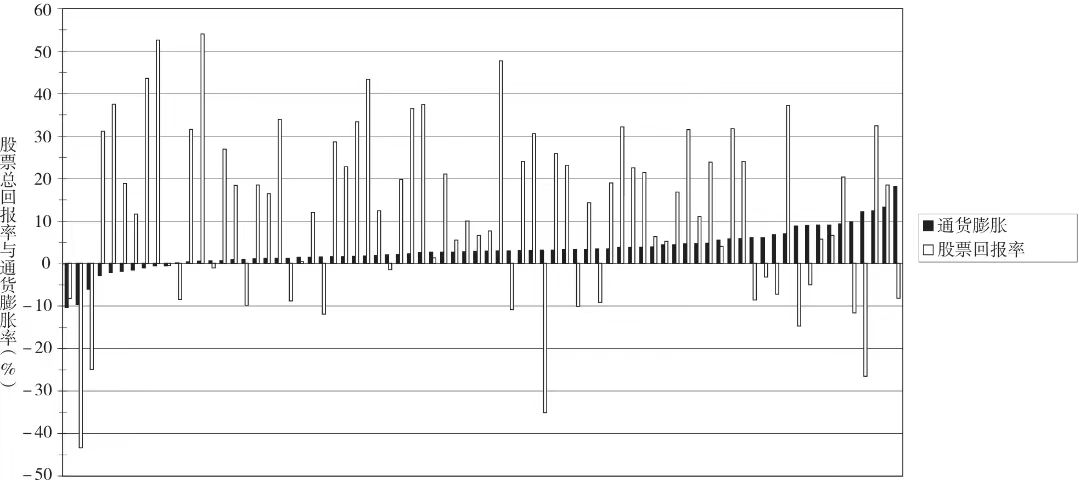
\includegraphics[width=\linewidth ,totalheight=0.95\textheight , keepaspectratio]{股票总回报率与通货膨胀率.jpg}
\caption{股票总回报率与通货膨胀率}
\end{figure}

上图显示了1926~2002年间,各年的通货膨胀与股票价格之间的关系,它不是按日历顺序,而是按通货膨胀率从低到高的顺序逐年排列的。当通货膨胀率为负数时(见图最左端),股票的表现很差;当通货膨胀较为温和时(大部分时段均如此),股票通常表现良好;但是当通货膨胀率达到非常高的水平时,股票的走势则起伏较大,经常会出现10\%以上的亏损。从图的左边可以看到,在消费品和服务价格下跌的各年,股票收益相当糟糕——股票总市值的下降幅度,最多可达43\%。如果通货膨胀率超过6\%,股票走势亦欠佳,如图右边部分所示。通货膨胀率超过6\%的情况出现过14年,其中8年股票市场的收益是负数;这14年的平均收益仅为2.6\%。

虽然温和的通货膨胀可以使公司把原材料的新增成本转移给消费者,但恶性通货膨胀则会造成灾难。它迫使消费者节衣缩食,并使经济各个环节的活动受到抑制。

历史给出的结果是明白无误的:自准确的股票市场数据在1926年出现以来,我们一共获得了64个五年期的数据(1926~1930年,1927~1931年,1928~1932年,等等,直到1998~2002年),其中有50个五年期(占总数的78\%)的股票收益,超过了同期通货膨胀率。这确实不错,但并不完美,因为在这一时期大约五分之一的时段,股票的收益没有赶上通货膨胀的速度。

\subsection{两种补救方式}
幸运的是,你可以在股票之外寻找防御通货膨胀的工具。在格雷厄姆最后一次修订本书之后,出现了两种为投资者普遍采用的通货膨胀保值工具:

REITs。这是“不动产投资信托”(Real Estate Investment Trusts)的缩写(其读音等同于“reets”),指那些拥有商业和住宅房产,并收取租金的公司。通过与房地产共同基金结合,REITs在通货膨胀保值方面干得相当不错。其中最佳的选择是先锋REIT指数基金,其他低成本的选择还有Cohen \& Steers Realty Shares、哥伦比亚房地产产权基金和富达不动产投资基金等。虽然REITs基金并不是一种十全十美的通货膨胀保值工具,但从长远来看,它多少能保护你免受购买力下降之苦,同时又不影响你的总体收益。

TIPS。这是“通货膨胀保值国债”(Treasury Inflation-Protected Securities)的缩写,它是美国政府于1997年首次发行的一种债券,其利率会随着通货膨胀率的上升而自动增加。由于有国家担保,所有的国债都不存在逾期不还(或不能支付利息)的风险。但TIPS还能保证你的投资价值不会受到通货膨胀的侵蚀。通过这样一种简便易行的方式,你就可以确保自己不会遭受购买力下降带来的财务损失了。

...

\section{防御型投资者的投资组合策略}
...

如果你不能承受风险,就应当满足于较低的投资回报——这是一个由来已久,且听起来十分合理的原则。由此可以得出这样的结论:投资者能够期望的回报,在一定程度上是与其承担的风险成正比的。对此,我们不能苟同。投资者的目标收益率,更多地是由他们乐于且能够为其投资付出的智慧所决定的:图省事且注重安全性的消极投资者,理应得到最低的报酬,而那些精明且富有经验的投资者,由于他们付出了最大的智慧和技能,则理应得到最大的回报。在1965年,我们曾说过:“在许多时候,买入那些‘廉价证券’的实际风险反而更小,其获得利润的机会,要比买入年息4.5\%的常规债券更大。”在接下来的几年间,由于利率的上涨,即使最高等级的长期债券的市值,也出现了大幅缩水,这更加证明了我们以上论断的正确性。


\subsection{债券与股票配置的基本问题}
我们已经以最简洁的方式,概括说明了防御型投资者的投资组合策略。他应当将其资金分散投资于高等级的债券和高等级的普通股。

作为一项基本的指导原则,我们建议这种投资者投资于股票的资金,决不能少于其资金总额的25\%,且不得高于75\%;与此相应,其债券投资的比例则应在75\%和25\%之间。这里的含义是,两种主要投资手段之间的标准分配比例,应该是各占一半。根据传统,增加普通股比重的合理理由是,持续的熊市导致了“低廉交易价格”的出现。反之,当投资者认为市场价格已经上升到危险高度时,则应将股票投资的比例减至50\%以下。【注意这里指的是高等级债券,一般垃圾债券或者收益率过低的债券(收益率相比较货币基金并无太大优势)是不在这里的讨论范围的,如果找不到好的高等级债券投资机会,那么可以将这里讨论的高等级债券换成现金仓位或者灵活的货币基金仓位也是可以的。——编者】

这种规范的原则说起来容易,做起来难——因为它与过度看涨牛市或过度看跌熊市这一人类的本性相抵触。要一个普通的股票投资者在市场超过某一点位时减仓,或在市场持续下跌后增仓,这似乎并不是一个切实可行的策略。正是由于普通投资者的相反操作(他们似乎必须这样去做),才使过去出现了大幅的上涨和下跌;而且(作者认为)未来还会发生类似的涨跌。

...

长期以来,我们一直认为,如果失去了债券这一参照物,我们就无法设定一个可靠的规则,以确定何时应将股票投资份额降至25\%这一最小比例,并在以后将其提升到75\%的最高比例。我们只能大体上要求投资者,不要轻易地让其股票投资超过资金总额的50\%,除非他充分确信,其股票持仓比例具有足够的合理性,而且可以坦然面对1969~1970年这样的股市大跌。按照1972年初的股价水平,我们很难看到有这样的强烈信心。因此,我们不建议,此时投资者的持股比例超过其资金量的50\%。但是,由于类似的理由,我们也很难要求投资者将其股票投资比例降至50\%以下,除非他自己的内心对当前的股价水平深感忧虑,并且满足于自己只有(比如)25\%的资金来参与未来可能出现的上涨。

因此,我们将向读者提出(两种投资)对半开的规则,尽管它看起来似乎过于简单。根据这一规则,投资者应在其实际操作中,保持对债券和股票的均等投资。比方说,如果股价水平使股票投资的比例提高到55\%,他们就应准备卖出十一分之一的股票,并将该笔资金投入债券,以恢复两者之间的均衡。反之,如果其持股比例仅为资金总额的45\%,他就应当考虑拿出十一分之一的债券,将其转为股票投资。

...

此外,真正的保守型投资者,将会对自己的一半资金在牛市中的收益感到知足;而在深陷熊市时,比照那些冒险型投资者的处境,他们也会从自己相对较好的境况中获得安慰。

虽然这种对半开的资金分配法则无疑是一种最简单的“万能”装置,但它不一定会取得最优的结果。...


\subsection{债券的构成}
投资者证券组合的债券投资部分,要解决两个主要问题:首先,他应该购买含税债券,还是免税债券?其次,他应该购买短期债券,还是长期债券?...

至于应选择长期债券还是短期债券,则是另外一个问题,即投资者是否想确保其债券的交易价格不会出现下降?如果是,那么其代价是:(1)较低的年收益率;(2)放弃债券本金部分可能出现的升值。我们认为,关于这一问题的讨论,最好是在第8章(投资者与市场波动)进行。

在过去的许多年内,个人投资者只能合理地选择购买美国储蓄债券。这种债券的安全性是无疑的(包括过去和现在);它们的收益要高于其他最优级别的债券投资;它们用提前取款和其他便利,极大地增加了它们的吸引力。在本书以前的版本中,我们用完整的一章(美国储蓄债券:投资者的福音)来介绍这一内容。

正如我们将要说明的那样,美国储蓄债券仍然具有某些独特的优点,因而对任何个人投资者来说,都不失为一种可取的投资方法。对于一个只拥有少量资金(比如,10 000美元以内)的投资者来说,购买此种债券仍然是其最便利且最佳的选择。但是,拥有更多资金的投资者也许会发现,其他的投资工具更有吸引力。

我们将列举一些值得投资者关注的债券类型,然后对它们的一般性质、安全性、收益、市场价格、风险、所得税状况以及其他相关特征分别予以简要的说明。

\begin{enumerate}
\item E系列和H系列的美国储蓄债券 ...
\item 其他的联邦政府债券 ...
\item 州债券和市政债券 ...
\item 公司债券 ...
\end{enumerate}



\subsubsection{高收益债券的投资}
如果肯在债券安全性上有所让步,投资者可能会从其债券投资中获得更高的收益。历史经验表明,就普通投资者而言,规避此种高收益债券不失为明智之举。尽管就总体而言,这种债券的收益要高于高等级债券,但它们会使所有者面临各种不利的风险——既包括令人心烦的债券价格下跌,也包括实际的违约(是的,低等级的债券经常会带来廉价交易的机会,但成功地开发需要进行专门的研究和拥有专门的技能)。

...
\subsubsection{作为债券替代物的储蓄存款}
现在,投资者可从商业银行或储蓄银行的储蓄存款(或银行定期存单)中,获得与短期高等级债券相等的收益。今后,银行储蓄账户的利率可能会有所下降,但目前仍不失为个人投资短期债券的一种很好的替代品。

\subsubsection{可转换债券}
相关讨论见第16章。关于该债券价格波动性的讨论见第8章:“投资者与市场波动”。

\subsubsection{赎回条款}
在本书以前的版本中,我们曾就这一问题长篇讨论,因为这种做法对投资人相当不公平,却从未引起足够的注意。通常情况下,债券在发行不久后即可赎回,其赎回价值略高于其发行价——比如,只有5\%。这意味着,当基准利率出现剧烈的波动时,投资者必须自行承担负面冲击,但是几乎无法使自己获得有利变化带来的好处。

例如,美国煤气和电力债券就是一个典型例子——期限100年,票面利率为5\%。该债券于1928年以101美元的价格向公众发行。4年后,在恐慌的氛围下,这一优质债券的价格跌到了62.5美元,收益率为8\%。到了1946年,经过一轮强劲反弹后,此类债券出售时的收益仅为3\%,因此其5\%的利率的对应价格应该接近160美元。但此时,该公司利用其赎回条款,仅以106美元的价格将其赎回。

这种债券发行合约中的赎回条款,几乎是公然宣称:“我总是赢家,而你总是输家”。在其问世很久以后,债券购买机构开始拒绝接受此种条款;近年来,大多数长期高息债券通常禁止发债机构在发行后的10年,乃至更长的时间内赎回该债券。这种做法仍然会有碍于债券价格的上涨,但已经比较公平了。

从现实的角度来说,我们建议长期债券的投资者宁肯收益率低一点,也要确保购买的债券是不可在短期内赎回的,其赎回期应在债券发行20~25年以后。同理,折价买进低息票率债券,要比购买息票率较高但大致按票面价发行且短期内即可赎回的债券更有利。因为,折扣部分(例如,息票率为3.5\%的债券,按面值的63.5\%出售时,其收益率可达7.85\%)足以保护赎回行为造成的不利。

\subsection{不可转换的优先股}
首先,我们对优先股的一般特点作若干说明。真正好的优先股可能且确实存在,这种投资工具是好的,但本质上是不好的。优先股的安全性,来自其发行公司支付普通股股息的能力和意愿;一旦公司董事会决定不分配普通股息,或公司没能力分配股息,优先股就会变得岌岌可危,因为在不支付普通股息的情况下,公司的董事们亦无义务偿付优先股。此外,优先股通常只能够获得固定比率的股息。因此,优先股持有者既没有债券持有人(或债权人)的法定求偿权,也不能像普通股股东(或合伙人)那样分享公司的利润。

在经济萧条时期,优先股在法律地位上的这种缺陷,会不断地暴露出来。只有很少的优先股,才有足够的实力来始终确保自己的投资地位。经验告诉我们,只有因暂时的危机致使优先股的价格跌至不合理的价位时,才可买入这种证券。(此时,它们也仅适合那些进取型的投资者,而非保守型的投资者。)

换言之,这种证券只可以按照廉价的交易条件买进,要么就干脆不买。以后,我们还将讨论可转换证券以及具有类似优先权的证券——某些特殊条款使它们有可能分享公司的利润。这些证券一般不会被纳入到保守的投资组合中去。

优先股还有另一项值得一提的特点:其税收地位更适合公司投资者,而不太适合个人投资者。公司获得的红利只需按照其总额的15\%缴纳所得税,而其利息收入则须按全额纳税;自1972年以后,公司的税率高达48\%。这意味着,公司每收入100美元的优先股股息,只需缴纳7.2美元的税金;而每收入100美元的债券利息,则须缴48美元的税金。另一方面,个人投资者优先股投资的收入和利息收入须缴纳的税率完全相等,直至近年才出台了一些小额的减免。因此,严格说来,公司投资者应该购买优先股,而须交纳所得税的个人投资者,则应购买免税的债券。

\subsection{证券的类型}
这里讨论的债券和优先股这两种证券形式,均易于理解,而且较为简单。债券持有人可以按固定利率得到利息,并在约定的日期偿还其本金。优先股的所有者可以按固定利率收到股息,但不能得到更多的股息——可在普通股之前得到股息。优先股的本金价值是没有到期期限的。(优先股的股息是可以累积的,也可以是非累积的;优先股股东可以拥有投票权,也可以不拥有投票权。)

以上是它们的一般特性,而且这两种形式的证券比比皆是。但不可否认,还有一些与其颇有差别的证券。其中最著名当属可转换的同类债券和收益债券。后者只有在其发行公司有利润时,才支付利息。(其利息可以累积,从公司未来的利润中支取;但累积期限通常仅限于3年。)

公司应当更多地运用收入债券的融资方式。在历史上,这种债券起初是在铁路重组活动中得到大规模运用,因而往往是与财务上的弱势地位和投资不利等因素紧密相关的——这正是许多公司不愿采用这种融资工具的原因。但这种证券实际上是很有优势的,特别是与近年大量发行的优先股相比,它们可作为替代品。这种证券的最大好处是,利息可以冲抵应税收入,从而可以使该证券的资本成本减少一半。对投资者而言,这种债券具有以下优点:(1)只要发行公司有利润,他就可以无条件地获得利息;(2)如果发行公司没有利润或不支付利息,除了破产保护以外,他还有其他的保护形式。收益债券的条款可以灵活商定,以使债权人和债务人均感到满意。(当然,也可以包括转换权在内。)人们总是乐于接受安全性较差的优先股,而拒绝接受安全性更优的收益债券,这充分地说明,华尔街总是存在着一些传统的做法和习俗,而无视在新的条件下需要新的观点。随着每一次新的乐观和悲观情绪的潮起潮落,我们会忘记历史并抛弃一些久经考验的原则,但是,却往往会顽固地坚持自己的偏见,并对其深信不疑。


\section{第4章点评}
你的投资组合应当承担多大的风险?

格雷厄姆的见解是,这首先取决于你是何种类型的投资者,而不是取决于你拥有怎样的投资品种。要成为一个聪明的投资者,有两种做法:

\begin{itemize}
\item 对一组由股票、债券和共同基金构成的动态投资组合,进行不断的研究、筛选和监控。
\item 或者,以某种自动的方式,创建一个恒久的投资组合,不再付出更多的努力。
\end{itemize}

格雷厄姆把第一种做法,叫做“积极的”或“进取的”的方法,它需要投入大量的时间和精力;而“被动的”或“防御型的”投资策略,无须花费多少时间,但要求投资者始终不为市场喧嚣所动;正如投资思想家查尔斯·埃利(Charles Ellis)表明的那样,积极的方式是劳心费力的,而防御型的方式则要求控制好自己的情绪。

如果你时间充裕,具有高度的竞争性,像一个球迷一样乐此不疲,而且对智力挑战颇有兴趣,那你不妨采用积极的路线。如果你总是觉得太过匆忙,渴望简单的生活,且不愿为金钱操心,则较适合被动的投资方式。(有些人也许更愿意把这两种方式结合起来,从而创建一个以积极为主被动为辅的投资组合;反之亦然。)

这两种方式同样明智,无论采取何种方式均可取得成功。但前提是,你必须对自己有深入的了解,从而采用适合自己的方式,并在自己的整个投资生涯中坚持下去,而且善于控制自己的投资成本和情绪。格雷厄姆对主动投资和被动投资的区分再次提醒我们,财务风险并非只存在于大多数人所关注的地方(经济形势和投资品种),而且也存在于我们的内心。

\subsection{是勇猛出击,还是防守}
那么,防御型投资者应当怎样入手呢?首先,而且是最基本的决策是,确定股票投资与债券和现金的分配比例。(请注意,格雷厄姆将这部分论述放在通货膨胀的章节之后,是为了让你事先了解,通货膨胀是你面对的其中一个最危险的敌人。)

最突出的一点是,格雷厄姆关于股票和债券资产分配的讨论中,根本没有提到“年龄”这一字眼。这使他与时下流行的庸俗看法区别开来。后者认为,你所承担的投资风险,主要取决于你的年龄。有一种传统的经验公式认为,你的股票投资所占的百分比,应当是100减去你的实际年龄,其余部分则应该以债券和现金的形式持有。(假如你28岁,应当将72\%的资金投资于股票;如果是81岁,则只应把19\%的资产投在股市。)像其他所有时髦说法一样,在20世纪90年代末期,这种观点曾风靡一时。1999年,一部通俗著作甚至宣称,如果你不到30岁,你可以把90\%的资金投入股市——即便你的风险承受力很“薄弱”!

除非你把自己的智商数减去100,否则,你一定会发现此类建议有什么地方不对。为什么你的年龄应当决定你可以承受多大的风险?一个拥有300万美元、丰厚的退休金和一群子孙的老太太,把她的大部分资产投资于债券的做法,无疑是愚蠢的。她已经拥有不菲的收入,而她的孙辈(他们最终将继承她的遗产)未来还有几十年的投资生涯。另一方面,一位年仅25岁,但正攒钱准备结婚买房的年轻人,也决不会打算将其全部资金投入股票。一旦股票市场上演高台跳水,他既没有债券的收益来弥补其损失,也没有钱以备不时之需。

此外,无论你多么年轻,你都可能会突然需要一大笔钱——不是在40年以后,而是在40分钟以后。在毫无先兆的情况下,你可能会失业、离婚、身受伤残,或遭受什么天晓得的意外。这些意外会突袭任何人,不管其年龄几何。每个人都应当将其资产的一部分,以现金的形式存放在无风险的安全地方。

最后,有些人正是因为股票市场的下跌,而终止其投资的。心理学家指出,大多数人都不善于预测自己将来遭遇令人沮丧之事时会感觉如何。当股票每年上涨15\%或20\%时(就像其20世纪80年代和90年代那样),不难想象,你会认为,你将与你的股票厮守终生。但是,当你看到你的每一美元投资,都缩水成了一毛钱时,你就很难抗拒将其变成“安全的”债券或现金的诱惑。因此,许多人不是买进并持有其股票,而是以贵买贱卖的痛心结果告终。正因为能够在熊市中有胆量坚守股票的投资者少之又少,格雷厄姆才坚决要求,每个投资者都至少应保持将资产的25\%投资于债券。他认为,投资于债券的这部分缓冲资产,将使你有勇气在股市不景气时,继续持有其余的股票。

为了更好地理解你可能承担的风险,不妨审视一下自己生活的基本环境:什么时候会出现新的情况,什么时候情况会发生变化,这些情况将如何影响到你的现金需求:

\begin{itemize}
\item 你是单身还是已婚?你的配偶或同居者以何为生?
\item 你已有或将会有子女吗?他们的学费什么时候会成为家庭的必要开支?
\item 你会继承一些财产吗?抑或你还要赡养年迈或有病的父母?
\item 哪些因素会对你的工作带来负面影响?(如果你供职于一家银行或建筑公司,利率的突然跳升可能会令你失去工作;如果你供职于一家化工企业,油价的飙升可能是一个坏消息。)
\item 如果你自己从事经营,与你的生意类似的企业,能够存续多长时间?
\item 你需要你的投资所得,来补贴你的日常开支吗?(一般说来,债券可以补贴你,而股票则不能。)
\item 考虑到你的薪水和开支情况,你可以承受多大的投资损失?
\end{itemize}

如果在审视了所有这些因素之后,你觉得自己可以承担拥有较多股票的较大风险,那么你就可以按照格雷厄姆给出的最低比率(25\%),来持有债券和现金。如果不是这样,你最好还是卖掉你的大部分股票,按照格雷厄姆给出的最高比率(75\%),来持有债券和现金。(要知道自己是否应百分之百地持有债券,请参见本书随后的专栏内容。)

一旦你确定了资产配置的最终比例,就不要轻易改动,除非你的生活状态出现了重大变化。既不要因为股市的上涨而加大其投资比例,也不要因为其下跌而更多地卖出。用约束取代猜想,这正是格雷厄姆投资法的精髓。...


\subsection{为什么不能把全部资产投资于股票}
格雷厄姆奉劝你投入股市的资金,永远不要超过自己总资产的75\%。但是,是不是每个人,都不适合把全部资金投入股市呢?对极少数投资者来说,全额投入也许是可行的。如果你属于下列群体,你也许可以这样做:

\begin{itemize}
\item 已经为自己的家庭准备好至少一年生活所需的全部资金
\item 准备在未来20年一直坚持投资
\item 已经成功度过2000年开始的熊市
\item 没有在2000年开始的熊市期间卖出股票
\item 在2000年开始的熊市期间,买入了更多的股票
\item 已经阅读了本书的第8章,并且已开始执行约束自身投资行为的正式计划

\end{itemize}

除非你确实通过了以上诸项测试,你决不能把自己的钱全部投入股票。在上一轮熊市中曾经陷入恐慌的人,在下一轮熊市仍将再次恐慌,并会因为没有债券和现金作为缓冲而深感懊悔。

\subsection{债券投资的细节}
在格雷厄姆的时代,债券投资者面临的基本选择是:购买免税的还是应税的债券?购买短期的还是长期债券?如今还需增加一项:购买债券还是债券基金?

购买免税债券还是应税债券?除非身处最低的纳税等级,否则,你必须将你退休账户以外的资金全部投入免税债券;不然的话,你的许多收益将被国税局拿走。...

购买短期债券还是长期债券?债券与利率的关系,就像一个跷跷板的两端:如果利率上扬,债券的价格就会下降,尽管短期债券的下降幅度远低于长期债券。另一方面,如果利率下跌,债券价格就会上涨,而且长期债券的上涨幅度会大于短期债券。你也可以通过购买5~10年到期的中期债券来缩小这种差别。这种债券既不会在利率飙升时大幅上涨,也不会在利率暴跌时一蹶不振。对大多数投资者来说,中期债券是一种最简单的选择,因为它可以使你不再为猜测未来利率的走势而烦恼。

购买债券还是债券基金?债券通常是以10 000美元为单位出售的,而你需要购买至少10种债券,才能将某种债券的违约风险分散掉。除非你至少有10万美元的投资,否则,购买单个债券的做法是不可取的。(惟一的例外是美国长期国债,因为它是由美国政府担保的,没有违约的问题。)

债券基金可以方便、廉价地提供分散化的好处;而且可以每月拿到利息收入,然后按照现行利率将其再投入该基金,且不收手续费。对于一般投资者来说,债券基金显然要优于直接购买单个债券(国库券和某些市政债券是一个主要的例外)。...


\subsection{其他债券投资}
怎样才能从你的现金中挤出更多的收益?聪明的投资者应当考虑,跳出银行定期存单和货币市场账户之类的传统工具(它们近年来的收益太低了),转向以下现金投资品种:

\begin{description}
\item[各种国债] 作为美国政府的债务,这些债券实际上没有违约风险,因为山姆大叔用不着赖帐——它随时可以通过增税或多印钞票来还债。...
\item[储蓄债券] 与国债不同,储蓄债券是不可交易的;你无法把它卖给其他投资者。如果提前支取,你还会损失三个月的利息。...
\item[抵押证券] 它是由全美数千种抵押贷款打包形成的,由联邦国民抵押贷款协会(“房利美”)或政府国民抵押贷款协会(“吉利美”)这类机构发行。然而,它们没有美国财政部的担保,因而其收益率定得较高,以体现其较高的风险性。当利率走低时,抵押债券通常会跌得更凶,但利率上升时也涨得更猛。...

\item[年金] 这种类似于保险的投资,可以帮助你把当前需缴纳的税金递延到将来,并在你退休后为你提供收入流。固定年金的收益率是固定的,而可变年金的收益率是浮动的。...

\item[优先股] 优先股是身兼两种缺点的投资。一是安全性不如债券,如果公司破产,其偿还权排在债权人之后。二是获利潜力低于普通股,因为如果利率下降或公司信用级别改善,发行公司通常会“赎回”或强行回购这些优先股。而且发行公司支付的股息,不能像其支付的债券利息那样,从应税利润中扣除,冲抵一部分所得税。...
\end{description}

 

 
\section{防御型投资者与普通股}
\subsection{普通股投资的优点}
在本书1949年的第一版中,我们发现,必须在此加入一段详细的解说,才能说明所有的投资组合,均须包含相当一部分的普通股。人们通常认为,普通股具有高度的投机性,因而是不安全的。股市曾经从1946年的高位经历了一次深幅下跌,但投资者们并没有因其价位更趋合理而被吸引,反而因其下跌造成的负面效应而心有余悸,丧失了对股权资产的信心。我们已对股市后20年的逆转进行了阐述:股价的大幅上升,使股票成为这一时期最安全且获利最丰的投资品种,但目前股价已被推升至历史最高水平,其中已蕴含了大量的风险。

我们关于1949年的股票市场的评论,可以归结为以下两点。首先,股票很大程度上使投资者得以免受通货膨胀的损失,而债券却完全不能提供这种保护。普通股的第二个优点在于,它可为投资者提供较高的多年平均回报;这不仅来自其较优质债券利息更高的平均红利水平,也来自因未分配利润的再投资而产生的市场价值上扬的长期趋势。

虽然这两项优势十分重要,而且确实令普通股的收益在过去很长一段时间,远远超过了债券,但我们仍然会继续提出如下警告:如果投资者以过高的价格买进股票,这些优势就会烟消云散。1929年的情况显然就是这样——此后经过25年,市场才恢复了元气(1929~1932年的股市出现了大幅跳水)。由于价格过高,1957年,普通股再次失去了其传统的股息收益率高于债券利率的优势。今后,通货膨胀和经济增长因素是否能够弥补这一重大转变带来的差距,仍将有待观察。

1971年年底,道琼斯指数已达900点,读者显然知道,我们对此点位的普通股没有多大兴趣。根据已经给出的理由,我们认为,防御型投资者不能忍受不在其投资组合中持有一部分普通股,虽然这只是一种两害相权取其轻的做法,因为全部持有债券的风险更大。

\subsection{普通股的投资规则}
对于防御型投资者而言,挑选普通股是一件相对容易的事情。在此我们给出四项可资遵循的规则:

\begin{enumerate}
\item 适当但不要过分分散化,你的持股数应限制在最少10只,最多30只不同的股票之间。
\item 你挑选的每一家公司应该是大型的、知名的,在财务上是稳健的。这些形容词必然会有一定的含糊性,但其基本意义是十分清楚的。关于这一问题的进一步讨论见本章的结尾部分。
\item 每一家公司都应具有长期连续支付股息的历史。(在1971年,道琼斯指数的成分股均满足这一条件)。具体说来,我们建议连续支付股息的历史,至少应该从1950年开始。
\item 投资者应将其买入股票的价格限制在一定的市盈率范围,其参照的每股收益,应取过去7年的平均数。我们认为,针对这一平均数,其市盈率应控制在25倍以内;如果是过去12个月的利润,则应控制在20倍以内。但这一限制会把所有最强势且最受欢迎的股票,排除在我们的投资组合之外。实际上,这将把几乎所有的“成长股”都排除在外,而这些股票正是过去若干年来股市的最爱,无论是投机者还是投资者均对其趋之若鹜。为此,我们必须对这种彻底的排除给出理由。
\end{enumerate}



\subsection{成长股与防御型投资者}
所谓“成长股”,是指那些在过去每股收益增长显著超过所有股票的平均水平,并且预计未来仍将如此持续下去的股票。(某些专家会说,真正的成长股至少会在未来10年内,每股收益翻一番,就是说,其年复合增长率为7.1\%。)显然,这样的股票是值得购买和拥有的,只要其价格不是太高。当然,也存在着问题,因为相对当期利润而言,成长股的价格一直都很高;相对于过去某一时期的利润而言,其市盈率更高。因此,在成长股投资方面带来很大的投机成分,从而使得此种投资的操作很难成功。

长期以来,IBM一直是成长股的龙头,而且确实为多年前买进并一直持有它的投资者带来了丰厚的回报。但是我们已经指出,这只所谓“最佳普通股”,曾在1961~1962年的6个月下跌中,折损一半;在1969~1970年间,也曾下跌几乎同样的幅度。其他成长股在逆境中的走势更糟;有时不仅股市在走低,这些公司的利润也在下降,由此会对持有这种股票的投资者造成双重打击。德州仪器是另一个可以佐证这一观点的良好例子:该股在6年间,从5美元涨到256美元,其间没有支付过一次股息,而其每股收益从40美分上升到3.91美元。(请注意,其股价的上涨幅度,相当于利润上升幅度的5倍;这是此类热门股的一般特征。)但两年以后,其利润下降了近50\%,股价则下降了五分之四,跌至49美元。

从以上例子读者可以看出,我们为什么会认为,对于防御型投资者来说,成长股的不确定性过高、风险过大。当然,如果股票选对了,买入的价格适当,并且在巨大的上涨之后、可能的下跌出现之前将其卖出,则会出现奇迹。但对于一般投资者而言,这种事情是可遇而不可求的。与此相比,我们认为,那些不那么热门,因此利润乘数较为合理的大型公司,反而是一种对大多数投资者更为合适的选择,尽管它们看上去不那么光彩夺目。在关于投资组合选择的章节中,我们将进一步阐述这一观点。

\subsection{投资组合的改变}
目前,很多投资者会将其证券投资组合定期送检,以确定其是否具有某种改善的余地。显然,这已成为投资顾问为其客户提供的一项主要服务了。几乎所有的经纪公司都可以提供相关建议,而且无需特别收费,以此来争取其他收费业务。也有一些经纪公司是以收费的方式提供该服务的。

我们的防御型投资者也应当寻求这种改进投资组合的建议——至少每年一次——就像其初次投资时会寻求建议一样。由于他缺乏关于哪些顾问可以信赖的专业知识,因此只能找那些声望最高的机构,否则,他很可能会遭到一些“二把刀”的糊弄。重要的是,他必须向其提请咨询的每一个顾问,申明自己要坚持本章开头提出的几项选股原则。需要说明的是,如果一开始选定的股票组合很恰当,就没有必要对其进行频繁或大规模的改变了。

\subsection{美元成本平均法}
纽约股票交易所在推广“月度购买计划”方面,已付出了相当大的努力。这种计划要求,投资者每个月投入同样数额的资金买进一只或多只股票。它是所谓的美元成本平均法(定期定额投资法)这种“程式化投资法”的一种特例。在始自1949年的股市大幅上涨期间,这种做法的效果相当令人满意,特别是在有效防止投资者在错误的时间大量买入股票方面。

露西尔·汤姆林森(Lucile Tomlinson)对这种程式化投资法进行了全面的研究。她以构成道琼斯工业指数成分股为样本,计算了美元成本平均法的效果。她的检测覆盖了23个十年期:头一个十年截止于1929年,最后一个十年截止于1952年。每一项检测都给出了期末或此后5年的利润情况。第23个购买期末的平均利润达21.5\%——股息不包括在内。显然,其中有些时期,投资者的股票市值会出现明显下降。汤姆林森小姐以如下惊人之语,结束了对这种极其简单的投资法的讨论:“无论证券价格出现怎样的波动,这种投资法都能使人满怀信心地取得最终的成功;迄今为止,尚无任何可与美元成本平均法相媲美的投资法问世。”

人们也许会对这种方法提出以下质疑:此法虽然言之有理,但实际上却很不现实,因为能够在连续20年内,每月拿出同样数额资金来购买普通股的人,实在少之又少。在我看来,这种显而易见的质疑近年来已不那么有力了。作为储蓄投资计划的必要成分,普通股已获得人们广泛的认同。因此,就像连续不断地买进美国储蓄债券和人寿保险一样,系统而一贯地购买股票,也不会对投资者造成多少心理和财务上的困扰了,后者可以看成是对前者的补充。如此购买股票,虽然每月投入的金额不大,但20年下来或者更长,其总量会相当可观,对投资者的意义也相当重大。

\subsection{投资者的个人情况}
...

这样,我们要再次重申本章开头提出的论断,这就是说,投资者应买入何种证券以及追求多高的投资回报率,不能以个人的资金多寡为依据,而要看自己在金融方面的能力,其中包括知识、经验和性格等。

\subsection{关于“风险”的说明}
一般说来,优质债券的风险要小于优质的优先股;而后者的风险,要小于优质的普通股。由此引申出人们对普通股的流行偏见,即认为股票是不“安全”的。联邦储备委员会1948年的调查报告证实了此种偏见的存在。我们要指出的是,在证券投资领域,“风险”和“安全性”具有两种不同的含义,会在人们的思想中造成混乱和歧义。

显然,到期不能支付利息和本金的债券是不安全的。同样,如果期望某只优先股甚至普通股会持续支付股息,结果其股息却被削减甚至取消了,那么它也是不安全的。如果某个证券持有人,很有可能不得不在其价格大大低于买价时抛售该证券,这也说明该证券含有风险。

不过,人们往往会把风险的概念,扩展到所持有的证券可能会出现下跌的情况,即使这种下跌只是周期性的和暂时性的,而且他无需在此时卖出。除了联邦储蓄债券,任何证券都可能出现此种情况;比起高等级的债券,普通股的波动幅度会更大。但从实际意义上来看,我们认为这并非真正的风险。持有住房抵押贷款的人,如果在不利的时机被迫出售房屋,将会遭受重大亏损。但是,在进行不动产抵押贷款时,人们通常不会以此来判定该项贷款是否安全;其安全性惟一的标准是,他能否按时还本付息。同理,判断一项普通的经营业务的风险时,要看其亏损的可能性有多大,而不是看其所有者被迫出售业务时情况会怎样。

在第8章,我们将明确提出自己的观点:就真正的投资者而言,单是市场价格的下跌,并不会导致他的亏损;因此,市场可能出现下跌这一事实,并不意味着他面临着实际的亏损风险。如果以合理的投资年限来衡量,一组精心挑选的股票投资组合,能为我们提供满意的整体回报,那么,这一组合实际上就是“安全”的。在此期间,其市场价值肯定会有所波动,但投资者同样有可能不会在成本价之下卖出股票。如果这一事实给投资造成了“风险”,那么,这种投资既应被称作是有风险的,同时也应被称作是安全的。假如我们仅把风险这一概念应用于价值损失(证券的实际售出,公司地位的严重恶化,或者更常见的是由于买价相对于债券的内在价值过高而出现了亏损),那么,这种混淆就可以避免。

许多普通股确实会有这种贬值的风险。但我们的观点是,一组经过适当挑选的投资组合,是不会含有此种风险的,至少其程度不会很高,因此不应仅仅因为其价格的波动而宣称“股票有风险”。不过,如果相对于股票的内在价值而言,买入价格过高,这种风险就会因此而呈现,即使出现严重下跌的股市在多年后能够收复失地。

\subsection{何谓“大型的、知名的和财务稳健的公司”}
上述引语出自本章前半部分,它被用来形容防御型投资者应该购买的股票类别。此外,这些公司还应当具有连续多年派发股息的记录。任何以形容词为基础的标准都总是含混不清的。究竟应如何来界定大型的、知名的和财务稳健的公司呢?关于最后一项限定,我们能够给出一个具体的标准——尽管有些随意性,但却是普遍接受的。对一家工业企业来说,其普通股的账面价值必须不低于其总资本(包括全部的银行债务)的一半,才称得上是财务稳健的。对铁路或公用事业公司来说,这一界限是不低于30\%。

“大型的”和“知名的”含有规模可观和行业地位领先的意思。这些公司通常被认为是“主要的”,而业内的其他企业则是“次要的”。当然,在成长股的投资者看来,成长股是一个例外。具体说来,我们不妨把“大型”界定为,公司目前的资产不低于5 000万美元,或营业额不低于5 000万美元。此外,作为一家“知名的”公司,其规模应位于所在行业的前四分之一或三分之一。

然而,过于执著如此随意性的标准则是愚蠢的。这一标准的提出只是参考性的。只要不违背关于“大型”和“知名”的公认含义,投资者为自己设定的任何标准都是可以接受的。由于这种定义固有的模糊性质,在那些适合防御型投资者的公司中,必定会有一部分被选中,另一部分则被淘汰。这种意见分歧和不同的选择不会带来不利影响。实际上,它对股票市场交易是有益的,因为这将使龙头股和次一级股票之间的差别,变得更微妙,层次更丰富。


\section{第5章点评}
\subsection{最好的防御就是有力的进攻}
经历了前几年股市的血雨腥风之后,防御型投资者为什么还要投资股市呢?

首先,要记住格雷厄姆所坚持的观点:你应该有多大的防御性,这并不取决于你对风险的容忍程度,而是取决于你愿意在自己的投资组合方面花多少时间和精力。如果你的方法恰当,投资股票就会像持有债券和现金一样轻松容易(在第9章我们将看到,你可以非常轻松地购买股票型指数基金)。

很容易理解的是,身处2000年开始的此轮熊市,你会为此感到焦灼,因此决定从此再也不买股票;这种反应是可以理解的。就像一句古老的土耳其谚语所说的那样——“被热牛奶烫过嘴之后,再喝酸奶也会用嘴去吹。”由于2000~2002年的股市崩溃是如此恐怖,许多投资者现在都觉得股票会烫伤自己。但是,殊不知,正是此种下跌已使股票市场的大部分风险得到了释放。在此之前,它确实是一杯烫牛奶,但现在已降到室温了。

由此可知,如今你是否应继续拥有股票,与几年前拥有的股票给你带来了多大的损失并无关系。如果股票的价格已变得相当合理,足以使你的财富今后得以增值,那你就应当购买它们,而不论其是否曾令你在不久前亏损过。尤其是在当今债券的收益率很低,从而减少你未来的投资回报的时候。

我们在第3章已经指出,与历史平均水平比较,2003年年初的股价只处于略高一点的价位。与此同时,从目前的价格来看,债券的收益率很低;因此,那些出于安全性购买债券的人,就好比一些烟民认为吸焦油含量较低的香烟可以避免肺癌一样。无论你是具有多大防御性的投资者——按照格雷厄姆的观点,即无论将持有的股票降低到多少;按照现在的观点,即无论将风险控制在多低的水平——为了保持今天的价值,你都必须至少拿出一部分钱来购买股票。

幸运的是,如今防御型投资者购买股票比以往任何时候都更容易了。目前有一种持久的自动投资组合系统,它可以使你毫不费力地把自己的钱,按月投入预先设定的投资品种,从此无须为选股浪费大量的时间。

\subsection{应该“买自己熟悉的股票”吗}
但是,首先让我们来看防御型投资者始终反对的一种观点:你无须为选股做任何功课。在20世纪80年代和90年代初期,“购买自己熟悉的股票”是当时最流行的投资口号。曾在1977~1990年间执掌富达麦哲伦基金,并获得共同基金最佳投资战绩的彼德·林奇就是这一信条最有力的鼓吹者。林奇认为,业余投资者拥有业内投资者已然忘却的一项优势,即知道如何去利用“常识的力量”。如果你发现一个很棒的新餐馆、一种新款汽车、牙膏或牛仔裤,或者你看到你家附近的一家店铺的停车场总是车水马龙,或一家公司的总部直到午夜电视剧播完后仍有人在加班,那么,你就会对某只股票形成一种专业分析师和基金经理人都不具备的亲身感受。正如林奇所指出的:“有了多次买汽车和照相机的经验,你会对商品的好坏以及是否好卖,形成自己的感觉……最重要的是,你比华尔街更早获知这一信息。”

林奇的规则——“如果利用自己的优势,投资于所熟悉的公司或产业,你就可以比专业人士做得更好”——并非毫无道理,而且多年来确实有成千上万的投资者从中受益。但林奇的这一法则,只有在你遵循以下结论时才有效:“找到一家看似有前途的公司只是第一步。下一步是对它进行研究。”他的真正意思是,在对一家公司的财务报表进行研究,并对其商业价值进行估量之前,决不能购买股票,无论其产品看起来有多棒,或他家的停车场停了多少辆顾客的汽车。

不幸的是,大多数股票投资者都忽略这一方面。

...


\subsection{填平补齐}
虽然股票市场总是日复一日地上下波动,防御型投资者却有办法控制这种无序的状态。你拒绝采取主动,而且从不假装具有预测未来的能力,这恰恰会成为你最有力的武器。你的每一个投资决策都是按既定程序自动做出的,因此你可以排除那种自以为能够预知市场走势的幻觉,不为市场力量所左右,无论其走势如何异乎寻常。

正如格雷厄姆指出的,“美元成本平均法”使你可以定期将一定数额的资金用于投资。无论股市已经(或者即将)上涨、下跌还是横盘,你都将按周、按月或者按季度买进股票。所有大型共同基金公司和经纪公司,都会为你提供安全的自动电子转账服务,这样你就不必动手填写支票,并为金钱的支出感到心痛了,正所谓“眼不见,心不烦。”

最为理想的美元成本平均法是投资于一组指数基金,从而将所有具有投资价值的股票和债券都一网打尽。这样的话,你就可以摆脱诸如预测股市的走向、了解哪些板块以及其中的哪些股票会表现最好之类的猜谜游戏。

假定你每个月可结余500美元,你可以借助美元成本平均法拥有三只指数基金。其中300美元投资于美国股票市场指数基金,100美元投资于外国股票指数基金,还有100美元投资于美国债券市场指数基金,这样你就可以确信囊括这个星球上几乎所有值得拥有的投资了。精确得像时钟一样,每个月你都会买进更多的股票;如果市场下跌,你预定的投资金额就会比前一月买入更多的股份;如果市场上涨,同样的金额所能买到的股份就会少于前一个月。以这种近乎自动的方式处置你的投资组合并持之以恒,就可以避免以下两种情形的出现:在市场似乎最具吸引力(实际上最危险)的时候,将手中的货币随意投向市场,抑或是在市场崩溃,股价确实便宜(但似乎更具“风险”)的时候,拒绝买进更多的股票。

根据一家颇有影响力的金融研究公司(Ibbotson Associates)的研究,如果你在1929年9月初,以12 000美元买进标准普尔500指数基金,十年之后你的手中将只剩下7 223美元。但是如果你以区区100美元起步,以后每月追加投入100美元,到1939年8月,你的资金就会增至15 571美元!这就是按照规则买进的威力——即便是面临大萧条这样有史以来最糟糕的熊市。

从1999年年底到2002年年底,标准普尔500指数出现了持续的下跌,但如果你以3 000美元的最低限额开立了一个指数基金账户,并每月追加投入100美元,那么你总计6 600美元的总投资,将亏损30.2\%——明显低于大盘41.3\%的跌幅。此外,你在较低价位的持续补仓,将使你在市场出现反弹时获得丰厚的利润。

最有利的是,一旦你以指数基金为核心,建立起一个具有永久性且自动导航式的投资组合,你就能够在面对所有相关市场的问题时,给出一个防御型投资者可能给出的最有力的回答:“我不知道,也不在乎。”如果有人问,债券的收益是否会好于股票,你只需回答:“我不知道,也不在乎。”——毕竟,你已经自动拥有这两个投资品种了。医疗保健股是否会令技术股黯然失色?“我不知道,也不在乎。”——你已经是这两类股票的长期拥有者了。谁会是下一个微软?“我不知道,也不在乎。”——只要它规模够大,你的指数基金就会买进它,而你将搭上这班车。明年外国股票是否会强于美国股票?“我不知道,也不在乎。”——如果真是这样,你将从中获利;如果不是,你将以较低的价格买进更多。

让你能够理直气壮地宣称“我不知道,也不在乎”这种永久性且自动导航式的投资组合会令你获得解放,再也无须为预测市场走势而殚精竭虑,尽管其他人仍沉溺于这种不切实际的追求中。承认自己对未来所知甚少,以及对这种无知的心安理得,正是防御型投资者最强大的武器。


\section{积极型投资者的证券组合策略:被动的方法}
“进攻型”或积极型投资者首先要遵循的策略,应该与防御型投资者基本相同,即以合理的价格,将其资金分别投入高等级债券和高等级普通股。他还会把他的一部分资金,投入其他种类的证券,但每一笔这种性质的投资,都必须有充分的依据。关于这一话题很难给出确切的论述,因为积极投资并不存在某种惟一的或理想的模式。其可供选择的领域十分宽广;其选择不仅有赖于投资者的个人能力和知识,而且同样地依赖于他的兴趣和偏好。

对积极型投资者最有用的总结是,指出他们不应该去做哪些事。他们通常不会购买高等级的优先股,宁愿将其让给公司购买者;他们也会回避那些等级较低的债券和优先股,除非其价格有相当大的折扣——以高息证券为例,其价格至少应比票面价值低30\%;至于低等级债券,其折扣还应大得多。他们宁愿让其他人购买外国政府债券,即使其收益率看起来相当不错。他们还会小心对待各种新发行的证券,其中包括很有吸引力的可转换债券和优先股,以及近期利润状况很好的普通股。
就通常的债券投资而言,积极型投资者会遵循与防御型投资者相同的原则,将其选择限于高等级的应税债券——其收益率现为7.25\%;以及优质的免税债券——其较长期限的品种的收益率目前为5.3\%。

...


\subsection{新股的发行}
以下段落全部来自本书的1959年版,未作任何改动,但增加了一些评论文字:

普通股的融资有两种形式:对已上市公司而言,它们会向现有的股票持有者按一定比例配售增发的股票。其发行价通常会低于现行市场价,因此其认购“权”会有一定的货币价值。这些股票通常会由一家或多家投资银行承销,但一般情况下,所有的新股会被行使认购权的人购买。因此,已上市公司的新增股票的发行,并不需要发行商的大力推销。

另一种形式是,原先的非上市公司向公众发行股票。这种股票大多是根据控股方的需要发行的,以使其可以在市场有利时兑现股票,并使自己的融资渠道多样化。(如前所述,这些企业往往会通过优先股的形式进行再融资。)这种发行活动方式周密,由于证券市场的固有性质,它必然会给投资大众带来诸多亏损和失望。其风险不仅来自进行圈钱活动的公司业务,而且来自使这种圈钱得以发生的市场环境。

20世纪初,美国的主要公司大批上市。随着时间的流逝,仍然由少数人把持的一流大公司已趋于消亡,因此股票一级市场越来越集中于那些规模较小的公司。不幸的是,在此期间,购买股票的公众已养成了一种根深蒂固的习惯,即偏爱那些大公司,对小公司则心存偏见。随着牛市的纵深推进,这种偏见——正如其他许多看法那样——会有所缓和;股票带来的横财和迅速致富的效应,足以令公众变得不再挑剔,就像它会激发他们贪婪的本能一样。与此同时,众多非上市公司会享受股票溢价发行的快感,尽管大部分公司的业绩并不怎么样——如果向前追溯十年或更长时间的话。

当这些因素交织在一起时,就会产生如下结果:在牛市的中途将出现第一批新股,其定价会较具吸引力,早期的购买者会从中获得巨额收益。随着市场升势的继续,这种类型的融资会愈演愈烈,而公司的质量会逐步走低,但其要价和实际成交价却越来越夸张。最后,一些不知名的小公司的发行价,会高出那些已上市多年的中型公司的当期价格,这正是牛市开始由盛而衰的一个相当可信的信号。(还应该补充一点,这些新股的发行,很少是由信誉较高的大型投行操作的。)

公众的粗心,以及承销机构只要有钱赚就愿意出售任何东西的做法,只会造成一个结果,即价格崩盘。许多时候,这些新股会从其发行价跌掉75\%甚至更多。雪上加霜的是,正如我们此前指出的那样,在股价的底部区域,公众对这些小盘股会非常厌恶,其程度就如他们当初买进时的狂热。因此,这些股票的价格会大大低于其实际价值,就像当初远远高于其价值一样。

能够在牛市期间抵御新股发行商的花言巧语,这是成为一个聪明投资者的基本条件。即使其中有一两只股票能够通过我们关于品质和价值的严格测试,不介入其销售仍不失为一项明智的策略。当然,经销商会指出这些股票具有许多市场优点,其中有些优点在当时看起来令人眼花缭乱。但所有这些都是投机气氛的一个组成部分。这是一种“快钱”。你从中赚到每一块钱时,都会赔掉两块钱,这还算是幸运的。

事实证明,其中有些股票是极好的购买对象。若干年后,在它们无人问津时,其真实价值会显现出来。

在本书的1965年版中,我们继续对这一问题进行了讨论:

总体来看,1949年以来的股市行为,并没有转到基于长期经验的分析,新一轮的新股发行仍然在照搬古已有之的老套路。在历史上,我们似乎从未见过像1960~1962年这样如此之多的新股发行,且质量如此之差,其股价的暴跌幅度又如此之大。从整体上看,股票市场能够如此迅速地从这场灾难中缓过来真是一个奇迹,这使我们不由想起很久以前的1925年佛罗里达房地产崩盘后类似的情形。

在当前的牛市走到其终点之前,一定会重现新股疯狂发行的一幕吗?天晓得。但我们确信,聪明的投资者不会忘记1962年的教训,不会像其他人那样,去赚那些短线利润并承受随之而来的巨额损失。

...



\section{第6章点评}
无论是进取型(积极型)投资者,还是防御型投资者,知道哪些该做以及哪些不该做,这对于你的成功都是很重要的。在本章,格雷厄姆列举了进取型投资者不应做的事情。以下是针对如今的情况列出的。

\subsection{垃圾场的野狗?}
格雷厄姆把高收益债券称之为“二级债券”或“低等级债券”,今天,我们则称之为“垃圾债券”。在格雷厄姆的时代,散户投资者要想通过多元化的投资来分散其违约风险是非常麻烦的,且成本高昂。然而,如今超过130多家专门投资此种债券的基金;他们大量地吃进这些垃圾债券,并且持有10多种不同的债券。这种情况缓解了格雷厄姆关于其无法分散化的担心。(但他对高收益优先股的此种担心依然有效,因为在分散其风险方面,至今仍缺乏成本低廉且普遍可行的手段。)

自1978年以来,年均利率达4.4\%的垃圾债券市场曾多次出现过违约。即使如此,其年回报率仍可达到10.5\%,而当时10年期国债的年回报率为8.6\%。不幸的是,这些垃圾债券基金大都要收取高额的佣金,而且往往无法保证你的本金不受损失。垃圾债券基金也许适合那些已经退休,且试图增加自己的月收入以弥补退休金之不足,同时能够承受其价值波动的投资者。如果你在一家银行或金融机构工作,利率的大幅上升会使你的职位升迁受到影响,甚至威胁到你的工作。因此,由于垃圾债券在利率上升时的表现会好于大多数债券,也许可以将其作为一种对冲手段纳入你的401(k)账户。但对于聪明的投资者来说,垃圾债券只是一种可供选择的权利,并不是一种非买不可的义务。


\subsection{内外兼顾的组合}
格雷厄姆认为,外国债券与垃圾债券差不多,均非优质投资目标。但是,对那些具有较高风险承受能力的投资者而言,如今外国债券已变得较具吸引力了。目前大约有十来只共同基金,专门从事新兴市场国家(或第三世界国家),如巴西、墨西哥、俄罗斯、尼日利亚和委内瑞拉等国的债券投资。明智的投资者购买此类烫手资产的数量,通常不会高于其总资产的10\%。但新兴市场国家的债券,一般不会与美国股票市场同步运行,因此,它们属于那种不会随道指下跌而下跌的少数品种之一。如果你确实需要此种资产,可以考虑将其少量纳入你的投资组合。

\subsection{致命的短线交易}
正如我们在第1章指出的,短线交易,即持有股票的时间在几小时左右,是有史以来人类发明的最佳自杀武器。你的某些交易会赚钱,你的大多数交易会赔钱,但你的经纪人却永远会从中获利。
而且你急于买进或卖出某只股票的行为,也会降低你的收益。如果你一定要买入某只股票,你的出价就会比大多数卖家乐意接受的价格高出10美分。这一额外成本,被称作“市场冲击”(market impact),它虽然不会出现在经纪商的账面上,但确实要耗费你的真金白银。如果你过于急切地想购进1 000股股票,并因此驱使该股的价格上涨了5美分,你就会为此多支出一笔无形但却实实在在的50美元。另一方面,如果一个恐慌的投资者急于卖出其持股,并且以低于其最近的市场价抛售,这种市场影响成本便会再次令你蒙受损失。

就像受到多层砂纸的打磨一样,交易成本会使你的收益层层流失。买进或卖出一只小盘热门股的交易成本达2\%到4\%(“全程成本”,即一买一卖的成本,高达4\%至8\%)。如果你在某只股票上投入1 000美元,它就会使你在起步之前就付出40美元的代价;卖出这只股票,你还要支付另外4\%的费用。

哦,此外还有这么一件事:如果你只是交易而非投资,你就会把长期所得(应交纳资本利得税,最高税率为20\%)变成普通收入(其最高税率为38.6\%)。

把所有这些考虑进来,短线交易者至少需要获得10\%的收益,才能在一买一卖的过程中打个平手。单凭运气,每个人都能够碰上一次;但要经常性的获利,以补偿为此付出的高度紧张(以及由此带来的噩梦般的压力),这是不可能的。

成千上万的投资者对此进行了尝试,但结果是毋庸置疑的:交易越频繁,自己得到的就越少。

...


\subsection{早起的鸟儿被虫咬}
20世纪90年代,对投资大众毒害最烈的一种观点,莫过于那种声称申购IPO产品可快速致富的说法了。所谓“IPO”是指“首次公开发行”,即把公司股票首次出售给公众。...

遗憾的是,每出现一次像微软那样让你赚得盆满钵满的IPO,就会出现数千次令你亏损的IPO。两位心理学家(Daniel Kahnerman和Amos Tversky)的研究表明,人们在估计某种事件发生的概率或频率时,往往做判断依据的不是其实际发生的频率,而是自己对过去事例的印象程度。我们都想买到“下一个微软”,恰恰是因为我们错失了购买第一个微软。但我们却很容易忽略这样一个事实,即大多数IPO都是一些很烂的股票。要想获得上述天文数字的财富,你必须逮住IPO市场上每一只大牛股;由于这些股票十分稀少,这种情况是不可能发生的。最后,那些高收益的IPO股票,大多被专门的小团体拿走了,这个由投资银行和基金公司组成的小圈子,在这些股票出售给公众之前,就以所谓的“包销”价将其吃进了。此外,涨得最猛的股票,通常是一些小盘股,即使大机构也拿不到其新股;市场上根本没有足够的股票可供你去参与。

如果几乎像每一个投资者那样,你只能在这些IPO暴涨之后才能够买进的话,那么,你的结局会相当悲惨。假如你在1980至2001年间以新股上市头一天的收盘价,买进一只典型的新股,并持有3年,你的年收益率将低于市场23个百分点。

...


\section{积极型投资者的证券组合策略:主动的方法}
根据定义,积极型投资者将花相当多的注意力和精力,来获得比普通投资更好的结果。...


\subsection{普通股业务}
积极型投资者在普通股领域的特定业务,可以分为以下4个方面:

\begin{enumerate}
\item 低价买入,高价卖出
\item 购买仔细挑选出的“成长股”
\item 购买各种廉价证券
\item 购买“特殊”股票
\end{enumerate}


\subsection{一般的市场策略——不同时期的方法}
关于低价买入、高价卖出策略的可能性和局限性,我们留到下一章讨论。过去许多年里,这个聪明的想法看起来既简单又可行,至少从反映股市周期波动的市场走势图中可以一眼看出。我们已经痛心地看到,过去20年的市场行为并没有使这种业务建立在某种数学规律的基础之上。发生的波动尽管达到了较大程度,但是要想从这种交易中获利,必须拥有特殊的才能或“感觉”。这完全不符合我们对读者智力所作出的假设,因此,在我们推荐的方法中,必须排除基于此类技巧的业务。

在前文中,我们向防御型投资者提出的对半开方案,大致可以看作是最具体或最直接的方法——根据1972年的情况,我们可以向所有投资者推荐这一方法。但是,我们在普通股选择方面留下了很大(25\%~75\%)的余地,这种余地使那些对一般市场水平的风险或吸引力有强烈判断的人可以做出选择。大约20年以前,我们可以详细地探讨在普通股持股比重方面存在的一些明确方法。我们确信,这些方法具有实用性。时间的变化似乎使此类方法过时了,而且,想要根据1949年以来的市场格局决定新的买卖水平似乎站不住脚了。这一时间太短,无法对未来提供任何可靠的指导。

\subsection{成长股投资}
每一位投资者都喜欢选择几年内业绩超过平均水平的公司股票。成长股的定义是:不仅过去的业绩超过了平均水平,而且预计将来也会如此。因此,聪明的投资者重点选择成长股,似乎是惟一符合逻辑的做法。实际上,正如我们将要看到的,这一问题较为复杂。

确定哪些公司过去的业绩“超过了平均水平”,这只不过是一项统计任务。投资者可以从自己的经纪人那里获得50家或100家这样的公司。那么,他为什么不仅仅从这类股票中挑选出最看好的15种或20种股票,从而保证自己的股票组合获得成功呢?

这种简单的想法面临两种意料不到的复杂情况。首先,业绩记录很好而且看上去很有前途的普通股,其价格也相应很高。投资者即使对其前景的判断是正确的,也仍然有可能得不到好的结果。原因就在于,预期收益已经完全包含在他所支付的股价中了(或许,他支付的股价还超出了预期收益);其次,他对未来的判断有可能是错误的。一般情况下,公司的快速增长不可能永久持续下去。当一家公司已经获得了非常显著的扩张时,仅仅因为其规模扩大,就使它很难再取得以往的成就。达到某一时点,增长曲线就会平缓下来,而且许多情况下会转为下降。

显然,如果某人根据事后的判断将自己局限于几种选择的情况,那么从他的结果中将很容易看到,成长股领域的投资既有可能成功,也有可能失败。人们如何较好地判断这种投资的总体结果呢?我们认为,通过研究专门从事成长股投资的基金公司所获得的结果,就可以得出比较可靠的结论。《投资公司》(Investment Commpanies)这本权威手册(由纽约股票交易所的会员公司Arthur Wiesenberger每年出版一册),对大约120家这样的“成长基金”在一定期限内的年度业绩进行了计算。其中,有45家公司的记录长达10年或10年以上。在1961~1970年的10年间,这45家公司总体的平均收益为108\%,而同期标准普尔综合指数的收益约为105\%,道琼斯工业平均数的收益为83\%。 1969和1970年这两年,在126种“成长型基金”中大多数的业绩都不如标准普尔和道琼斯这两种指数。从我们以前的研究中,可以看到类似的结果。这就说明,与一般的普通股投资相比,对成长型公司股票的分散化投资并不能带来优异的回报。

根本没有理由使人相信,一个智力一般的投资者(即使投入了大量的精力)购买成长股的结果,会好于专门在这一领域投资的基金公司。显然,这些机构可以利用更多的智慧和更好的研究手段。因此,我们不赞成积极投资者通常所从事的成长股投资。在这种投资领域,极好的未来前景已经完全被市场发现了,而且已经通过当期的市盈率(比如,20倍以上的市盈率)得到了反映。(我们建议,防御型投资者股票购买价的上限为过去7年平均利润的25倍。这两个标准在大多数情况下都是一样的。)

成长股这一类股票的一个显著特点,就是其市场价格的波动幅度一般较大。对于历史悠久的大公司(比如通用电气和IBM等)而言,情况是这样的;对于历史较短、规模较小的成功企业而言,情况更是如此。它们证明了我们如下的观点:1949年以来,股市的主要特征是,一种高度投机性的因素进入了某些公司的股票之中,这些公司取得了非常显著的成功,而且,它们本身享有很高的投资信用级别。(它们拥有最佳的信用地位;而且,它们的借款利率是最低的。)这种公司的投资质量,或许在很多年内都不会发生改变,但是,其股票的风险特征却是依赖于股市变化的。公众对这种股票的热情越高,股价上涨的速度相对于其实际利润的增长就越快,同时,这种股票的风险也就越大。

读者可能会问,情况难道不是这样吗?普通股真正的巨额收益落到了下列人的手中,他们在早期对未来非常看好的公司投入大量的股本,并坚定不移地持有这些股份,直到其价值上涨100倍或更高。答案是肯定的。但是,从一家公司的投资中获取的巨额财富,几乎总是由下列人来实现的:他们与特定公司有密切联系(通过雇用关系和亲属关系等),从而使他们将自己大部分的资金以一种方式投入进去,并且在各种情况下都始终持有这部分投资——尽管一直都有许多似乎能按高价出售的机会在引诱着他们。没有这种密切的个人联系的投资者,会不断地面临着这样的问题:以这种方式投入的资金是否过多?每一次的价格下跌(无论事后证明这种下跌是多么短暂)都会加重这一问题,而且内部和外部压力都有可能迫使他去接受看上去已经不错的利润,但这一利润却大大低于最终能获取的巨额财富。



\subsection{推荐三个可用于“积极投资”的领域}
为了在长时间内获得比一般投资更好的结果,一种选择或操作策略必须具备两项优势:(1)它必须能达到基本稳健所要求的客观或合理标准;(2)它必须有别于大多数投资者或投机者采用的策略。根据经验和研究,我们推荐满足这些标准的三种投资方法。这些方法相互之间有很大的不同,而且每种方法都要求其分析者具有不同的知识和禀性。

...

\subsubsection{购买廉价证券}
我们对廉价证券的定义是:根据分析确立的事实,这种证券的价值似乎要大大高于其售价。这一类证券中,既包括售价低于面值的债券和优先股,也包括普通股。为了尽可能具体一些,我们假设真正的“廉价”证券显示的价值,至少要比其价格高出50\%。哪些事实能够证明存在如此巨大的差异?廉价证券是如何产生的?投资者又如何从中获利?

有两个标准可以用来寻找廉价普通股。首先是采用评估法。这主要是在对未来利润做出估计之后,再乘以与特定证券相适应的一个系数。如果得出的价值足以高出证券的市场价(而且假如投资者对所使用的方法有信心),那么他就可以将这种股票称为廉价股。第二项标准是私人所有者从企业中获得的价值。这种价值通常也主要由未来的预期利润决定——这种情况下得出的结果可能与第一个标准是一样的。但是在第二个标准中,更关注的可能是资产的可实现价值,尤其强调的是净流动资产或营运资本。

按照这些标准来衡量,当市场总体处于低价位时,大量的普通股就成了廉价股。(一个典型的例子就是通用汽车:1941年,其股价还不到30美元,只相当于1971年5美元的股价。它当时的每股收益比1971年还多4美元,支付的股息比1971年高出3.5美元以上。)的确,当期利润和近期前景都不太好,但是,通过对未来总体情况的冷静分析可以看出,公司的价值大大高于当时的市场价格。因此,在廉价证券市场表现出的勇气,并不仅仅来自于以往的经验,而且还依赖于合理的价值分析方法的运用。

从一般市场环境下经常发生的廉价交易情况可以看到,几乎所有的市场层面中也都同样存在着许多单个的廉价证券。市场喜欢小题大做,使普通的波动夸大为严重的倒退。即使只是缺乏一点兴趣或热情,也会使价格降到荒谬的水平。因此,我们可以看到,价格被低估有两个重要因素:(1)当期令人失望的结果;(2)长期被忽视或不受欢迎。

可是,如果单独来考虑的话,这两个因素都不可能成功地指导普通股的投资。我们如何确信,目前令人失望的结果的确只是短暂的现象?是的,在这方面,我们能够提供一些非常好的例子。钢铁股曾经以其周期性波动而闻名,精明的买主可以在利润低下时低价购买这些股票,等到繁荣年份将其出售,以获得丰厚的收益。

如果这是利润波动的股票所表现出的一致行为,那么在股市赚钱就很容易了。遗憾的是,我们可以说出许多这样的例子:利润和股价下降之后,两者并没有在随后自动出现大规模反弹。Anaconda电缆公司就是这方面的一个例子。1956年之前,该公司的利润一直都在快速上涨,当年的股价达到了85美元的最高位。随后6年内,利润出现了不规则的下降;股价于1962年跌到了23.5美元;而且,在1963年,它被母公司(Anaconda集团)以每股仅33美元的价格收购了。

这方面的许多经历表明,投资者要进行稳妥的投资,仅仅观察利润和股价的同时下跌是不够的。他还应该要求,过去10年或更长时间内的利润至少具有较好的稳定性(没有利润赤字的年份);同时,还要要求公司具备足够的规模和财务实力,以应对未来有可能出现的困难。因此,这里的理想状态是:一家著名大公司的股价,既大大低于其过去的平均价,又大大低于其过去平均的市盈率。这无疑会把许多公司(比如克莱斯勒)的赚钱机会排除在外,因为这些公司在股价较低的年份里,一般也伴随着较高的市盈率。但是,现在我们要明确地告诉读者(无疑,我们还将这样去做),“事后看到的利润”和“实际得到的利润”是不同的。我们十分怀疑,像克莱斯勒这样不稳定的公司,是否可以被我们的积极投资者加以恰当利用。

我们已经指出过,长期被忽视或不受欢迎是导致股价偏低的另一个原因。目前这方面的一个例子就是National Presto Industries公司。1968年牛市期间,它的最高股价为45美元,这只是当年每股5.61美元利润的8倍。1969年和1970年的每股收益都上涨了,但股价在1970年降到了只有21美元。这个价格还不到当年利润(记录)的4倍,而且也低于其净流动资产的价值。1972年3月,该股票的售价为34美元,仍然只相当于上一次报告利润的5.5倍,而且大约相当于增长后的净流动资产价值。

...

导致普通股价格偏低的第三个原因,有可能是市场没有了解公司的实际利润状况。这方面的一个典型例子就是北太平洋铁路公司——1946~1947年,该公司的股价从36美元跌到了13.5美元。公司1947年的实际利润接近于每股10美元。股价受到抑制,主要来自其1美元的股息。被忽视的另一个原因在于,铁路公司特定的会计方法,掩盖了公司的大部分盈利能力。

最容易识别的一类廉价证券是这样一种普通股:售价比公司(扣除所有优先债务后)的净营运资本本身还要低。这意味着,股票的买主根本没有支付固定资产(房屋和机器设备等)的价格,以及任何形式的商誉价格。公司的价值最终低于其营运资本本身这样的情况是极少发生的——尽管可以看到少数的几个例子。...


在1957年之前的许多年内,这种建立在分散化基础上的投资选择方法都能收到很好的效果。我们可以毫无保留地说,这是在发现和利用证券低估机会时的一种安全并有利可图的方法。可是,在1957年之后的整体市场上升时期,此类机会已非常罕见,而且许多可以利用的机会最终也只带来了少量的操作利润,有的甚至出现了亏损。1969~1970年的市场下跌,导致了新的一批“价格低于营运资本”股票的出现。在第15章介绍积极型投资者的股票选择时,我们将探讨这一类股票。

二类企业廉价证券的情况 我们所定义的二类企业,是指没有在重要行业中占据领导地位的企业。因此,这类企业通常都是自己业务领域的一些小企业,但是同样也包括非重点业务领域的一些主要企业。为了区别,任何已被称为成长股的企业,一般都不看作是“二类企业”。

20世纪20年代牛市强劲时期,人们一般不对行业领导者和其他上市公司做出区分——只要后者达到了一定的规模。公众认为,中等规模的企业有足够的实力渡过难关,而且它们比已有的大企业有真正更好的增长机会。可是,1931~1932年的萧条,给规模不是很大或内在稳定性不是很强的企业以沉重打击。有了这一番经历之后,投资者开始明显偏好行业领头羊,同时对处于次要地位的普通企业大多失去了兴趣。这意味着后一类企业的股价一般会比前者低许多(相对于利润和资产而言)。同时,这更进一步意味着,许多情况下,股价会下降到廉价股的水平。

当投资者拒绝二类企业的股票时,尽管这些股票的价格相对较低,但他们却认为或担心此类公司的前景不好。实际上,至少在下意识里,他们认为这些股票的任何价格水平都太高,因为它们是走向消亡的——正如1929年的类似理论,那时人们认为对“蓝筹股”而言,任何价格都不高,因为它们的未来前景是无限的。这两种观点都被夸大了,同时会带来严重的投资失误。事实上,与普通的非上市公司相比,规模中等的上市公司一般都称得上是大企业。我们没有正当理由认为:这类公司的业务将无法持续下去;并且在经历了经济特有的波动之后,这类公司的投资资本总体上不能获得较好的回报。

这种简要的分析表明,股市对二类企业的态度一般是不切实际的,因此,这会导致一般情况下出现众多的价格严重低估。正如我们看到的,二战时期及战后繁荣时期对规模较小的企业更加有利,其原因在于,通常存在的销售竞争被终止了,这样,小企业可以更快地扩展其销量和利润空间。因此,1946年的市场情况与战前的完全不同了。按1938年年底的股价和1946年的最高股价来看,道琼斯工业平均指数中大企业的股价在这一时期只上涨了40\%,而同一时期标准普尔指数中的低价股的涨幅超过了280\%。投机者和许多以自己的方式从事投资的人(众所周知,股民的记忆是短暂的),开始以高估的价格积极购买一些次要企业的新旧股份。所以,摆锤又明显地偏向了另一个极端。以前的二类股份绝大部分都能提供廉价交易的机会,而现在这类股份,绝大多数都因为人们的过度热情而被高估了。这种现象在1961年和1968年又以不同的方式出现了——这时的重点转向了更小的一些企业发行的新股,以及绝大多数受欢迎的领域的企业(电子企业、计算机企业和特许经营企业等)发行的股票。

正如人们所预料的,这些被高估的证券随后在市场上会出现大幅下跌。有时候价格的摆动将造成明显的被低估。

如果大多数二类证券通常都倾向于被低估,那么,投资者为什么会认为可以在这种情况下获利呢?因为,如果这种情况一直持续下去,投资者不是始终处在与购买这些证券时相同的市场状况吗?这个问题的答案有点复杂。廉价购买二类企业证券的巨额利润来自于许多方面。首先,股息回报比较高。其次,用于再投资的利润相对于支付的价格而言比较大,因此最终会影响股价。在5~7年内,这些优势会在精心挑选的股票中明显反映出来。第三,牛市期间,低价证券的价格一般也会比较高,因此,这会使一般的廉价证券的价格至少上升到一个合理水平。第四,即使在市场相对平淡的时期,也会不断出现价格调整过程,这样,被低估的二类证券至少会上升到这类证券通常应有的价格水平。第五,导致利润记录令人失望的许多特定因素,会因为新情况的出现、新政策的采纳和管理层的变动而得到纠正。


...

\subsection{一些“特殊”情况}
不久以前,这一领域几乎可以保证那些懂行的人获得可观的回报,而且几乎在任何一般市场环境下都是如此。对于一般公众而言,这实际上并非一块禁地。具有这方面天赋的人,可以在没有经过长期学术研究或学习指导的情况下掌握其中的窍门,并且成为能力很强的从业者。其他人能够敏锐地了解这种方法的基本可靠性,并且使自身依赖于一些聪明的年轻人(这些人管理的资金主要用于那些“特殊情况”。)可是,最近几年,由于一些原因(将在后面分析),“套利和特殊情况”这一领域风险增大,也更无利可图。也许几年之后,这一领域的条件会变得更有利。无论怎样,我们都有必要通过一两个例子,来简要说明这些业务的总体特点及起源。

“特殊情况”一般来自于大企业对小企业收购的不断增加,这是由于越来越多的管理层采纳了业务多元化的信条。如果一个企业想进入某一领域,人们经常认为采用收购现有公司的办法,比从头开始建立一个新公司的做法更好一些。为了使这种收购成为可能,以及为了得到小公司的大多数股东对交易的认可,收购企业总是要提出一个大大高于现有水平的价格。这种公司行为会给一些人带来具有诱惑力的盈利机会(这些人对该领域有所研究,并且有大量的实际经验来支持可靠的判断)。

就在几年以前,一些精明的投资者花大量的钱购买了破产铁路企业的债券。他们知道,铁路公司最终重组后,这些债券的价值会大大高于其购买成本。重组计划公布之后,出现了一个针对新发售证券的“发行前”市场。这些证券的售价必将大大高于购买旧证券的成本。尽管也存在计划未实现或被意外推迟的风险,但是总体上讲,这种“套利业务”都是非常有利可图的。

1935年的法律要求对公用事业控股公司进行拆分,这也带来了类似的机会。从控股公司转变为一群独立经营的公司之后,几乎所有这些企业的价值都大幅度上升了。

这里的根本原因在于,证券市场倾向于低估涉及任何复杂法律诉讼的证券。华尔街有一句古老的格言:“永远不要购买涉及法律诉讼的证券。”对于寻求短期购买行为的投机者而言,这可能是一个稳妥的建议。但是,如果公众采用这种态度,必然会使受影响的证券成为廉价投资机会,因为对这些证券的偏见会使其价格降到不恰当的低水平。

对特殊情况的利用是一种投资技巧,它要求的智力和操作都有些不寻常。或许只有一少部分积极型投资者才愿意从事这项业务,因此,这不是本书要深入分析的一种投资方法。

\subsection{我们的投资法则所具有的更广泛含义}
这里介绍的投资策略,首先依赖于投资者做出的选择:是想充当防御型(被动)投资者,还是想充当进取型(积极)投资者。实际上,积极投资者必须拥有大量的证券估价知识,才能把自己的证券业务看成一种事业。被动地位和主动地位之间,并不存在着一种或一系列中间概念。许多,或许大多数投资者,都想将自己置身于这样的一种中间地位;但我们认为,这种折衷态度更有可能带来的不是收获,而是一种令人失望的结果。

作为一名投资者,你不可能成为较好的“半个经营者”,并因此而期望你的投资带来相当于正常业务一半的利润。

根据这一推论,大多数证券所有者都应该选择防御型投资者这一类别。他们没有时间、决断力和精力,来像经营企业那样从事投资活动。因此,他们应该满足于现在从防御型证券组合中获得的优越回报(甚至是较低的回报);而且,他们还应该坚定地抵制不断出现的诱惑——为了增加回报,而偏离到其他道路上去的诱惑。

积极型投资者应该从事一些恰当的证券业务,即自己的知识和判断力足以应对这些业务;而且,按已有的商业准则来看,这些业务有足够好的前景。

在向这类投资者提供建议和忠告时,我们都力求采用此类商业准则。在向防御型投资者提出建议和忠告时,我们主要遵循(心理上和数学上的)三个要求:基本安全性,选择方法简单,以及有望获得满意的结果。利用这些标准,我们可以在所建议的投资领域排除几类证券(这些证券通常被看作是适合各种不同投资者的)。第1章列出了这些被排除的证券。

关于为什么要排除这些证券,让我们进行更全面的分析。我们建议,人们不要按“全价”购买三类重要的证券:(1)外国债券;(2)一般的优先股;(3)二类普通股。(当然也包括这几类证券的初始发行。)我们所说的“全价”,是指接近于债券和优先股面值的价格,以及大约相当于企业公允业务价值的普通股价格。大多数防御型投资者会回避这几类证券(无论价格如何);积极投资者只会按低廉的价格购买它们——我们定义的低价,是指价格不超过证券评估价值的三分之二。

如果所有的投资者都采纳我们给出的这些建议,情况会怎样呢?在本书前面章节介绍外国债券时,我们考虑过这一问题,因此,这里我们不再多说了。投资级优先股只会被一些公司(比如保险公司)购买,因为它们可以从所持股票的特殊所得税地位中受益。

在我们的排除策略中,二类普通股这一领域是最麻烦的。如果绝大多数投资者都是防御型投资者而根本不去购买它们,那么这一领域可能的买主将会十分有限。此外,如果积极型投资者只是在廉价水平购买它们,那么这些证券的售价必定会低于其公允价值,除非有一些不明智的人去购买它们。

这听起来非常严重,甚至隐约感到有些不道德。然而事实上,我们只是认识到了过去40年的大多数时间里这一领域实际发生的情况。在大多数时间里,二类证券的确会围绕某一中心水平(它大大低于其公允价值)而波动。有时它们的价格会达到甚至超过公允价值,但这只会发生在牛市的上升阶段,此时,实际经验中获得的教训,将会与按市场价格购买普通股的理性观点相抵触。

因此,我们的建议只是要求积极投资者应该认识到二级证券所处的客观现实,并且以此类证券通常的中心市场价格水平为指导,来确定自己的购买价。

然而,这里也存在着一个矛盾。细心挑选出的二类企业,完全有可能与行业领导者一样具有良好的前景。小企业缺乏的内在稳定性,完全可以借助于快速增长潜力来加以弥补。因此,在许多读者看来,把按全部“企业价值”购买二类股票说成是“不明智的”,这似乎并不符合逻辑。我们认为,实际经验是最有说服力的。金融领域的历史清楚地表明,一般而言,投资者如果想从二类普通股中获得满意的结果,就必须按低于其私人所有者的价值(按廉价条件)来购买它们。

最后一句话意味着,这一原则与普通的外部投资者相关。任何人,只要他能够控制二类企业,或者是作为一个群体中的一名成员而享有此类控制权,他就完全有理由把购买这些股票的行为,看成是在“密切关联企业”或其他私人企业的投资。企业本身的重要性越低,内部和外部投资者的地位,以及相应的投资策略之间的区别就越重要。主要的企业或领头企业的一个基本特征是,一种独立的股份通常相当于一种有控制权的股份。在二类企业中,独立股份的平均市场价值,会大大低于有控制权的股份。由于这样一个事实的存在,与主要企业相比,二类企业的股东和管理层的关系以及内部和外部股东的关系,一般都显得更加重要和更具有争议。

在第5章结尾我们曾经讲过,对主要企业和二类企业进行严格的区分是很困难的。居于两者之间的许多普通股,会显示出某种中间价格行为。有的投资者会以低于账面值或评估价值的小幅折价购买这种普通股——这些投资者认为,从理论上讲,它们与主要企业的股票只有很小的差距;而且认为,这种股票在不久的将来会完全达到主要股票的信用级别。我们认为,这种做法不是不符合逻辑的。

因此,在主要证券和二级证券之间不需要做出精确的区分。因为如果这样做的话,那么质量方面的较小差别,必然会导致应有的购买价之间出现重大差别。这种说法表明,我们承认普通股的分类存在着一个中间地带,尽管我们不赞成对投资者的分类也存在这样一个中间地带。这种明显的不一致是源于这样的原因:在某种证券上的看法出现一定程度的不确定性并不会带来巨大的损害,因为这些情况都属于例外,而且在这件事情上没有太大的利害关系。可是,投资者在防御地位和积极地位之间的选择,对他而言是极为重要的,因此,他不应该在这个基本决定方面模棱两可,或采取折衷做法。


\section{第7章点评}
\subsection{时机的选择并不重要}
在理想条件下,聪明的投资者只会在价格便宜时购买股票,在价格涨高时将其出售;然后以债券和现金的形式持有这些资金,直到股价再一次变得便宜时再去购买。一项研究表明,从1966年到2001年年底,持续持有的1美元股票最终将上涨到11.71美元。可是,如果你能恰好在每年中5个最坏的日子到来之前平仓的话,那么你最初的1美元将上升到987.12美元。

与市场上大多数的魔幻想法一样,这种想法也是基于一种戏法。你(或其他任何人)怎样才能确切地知道哪几天是最糟糕的——在这些日子到来之前?1973年1月7日,《纽约时报》对美国的一位高级金融预言家进行了专访。这位预言家督促投资者赶快购买股票:“现在绝对处在牛市时期,以往很少见到这样的情况。”这位预言家就是艾伦·格林斯潘,而且非常罕见的是,没有哪一个人像这位日后的美联储主席那样,在当天做出了完全错误的判断。后来的事实证明,自大萧条时期以来,1973年和1974年是经济增长和股市表现最不好的年份。

专业人士对入市时机的判断,会比格林斯潘更准确吗?“我认为,大部分下降压力都已经过去了,”2001年12月3日,R.M.Leary公司择时交易机构的负责人凯特·利里·李说道,“这正是你应该入市的时候。”她补充道——她预测2002年第一季度的股票“会表现得不错”。随后的3个月内,股票的回报仅有微小的0.28\%,比现金的回报还低1.5个百分点。

持此观点的并非利里一人。杜克大学的金融学教授进行的一项研究表明,如果你采纳最好的择时交易刊物(占总刊物的10\%)所提出的建议,那么,你在1991~1995年赚取的年回报率将是12.6\%。可是,如果你不听从它们的建议,而将资金投入到股票指数基金中去,那么,你将获得16.4\%的回报。

正如丹麦哲学家齐克果所指出的,只有回过头来才能理解生活,但是,生活必须往前走。回过头去看,你总能准确地了解应该何时购买股票以及何时出售股票。然而,你不能愚蠢地认为,在实际中自己可以随时判断应该在何时进入,在何时退出。在金融市场上,事后观察永远是完全清楚的,但是,事先预测必定是盲目的。因此,对大多数投资者而言,择时交易从实际上和心理上看都是不可能的。

\subsection{哪些股票会上涨}
正如宇宙飞船进入地球的同温层后会加速一样,成长股似乎也经常会脱离重心引力。我们来看20世纪90年代3种增长最快的股票的变化轨迹:通用电气、家得宝和太阳计算机系统公司。

从1995年到1999年,每家公司每年的规模和利润都在增长。从营业收入上看,太阳公司增长了一倍,家得宝公司增长了一倍多。根据Value Line公司提供的信息,通用电气的营业收入增长了29\%,利润增长了65\%。家得宝和太阳公司的每股收益几乎增加到了原来的3倍。

然而,其他的情况也在发生,这丝毫不会使格雷厄姆感到惊讶。这些公司增长得越快,其股价也越来越昂贵。当股价的上涨超过了公司的成长速度时,投资者最终总是会吃亏的。

如果其股票价格太高的话,一家优秀的企业并不是一个非常棒的投资对象。

股价上涨得越高,似乎就更有可能继续上涨。但是,这种本能的看法完全与金融物理现象的根本法则相抵触:公司的规模越大,增长速度就越慢。销售收入为10亿美元的公司,能够轻易地使自己的销售收入增加一倍;但是,业务量为500亿美元的公司到哪里去寻找另外500亿美元的业务量呢?

在股价合理的情况下,成长股值得去购买。但是,当其市盈率大大高于20或30倍时,再去大量购买就会有些不妙了:...

认为高增长能够永远持续下去的幻觉,并非只是发生在投资者身上。2000年2月,有人问北电网络(Nortel Networks)的首席执行官约翰·罗思,这家光纤行业巨头的规模会达到多大。“该产业正在以每年14\%~15\%的速度增长,”罗思回答说,“而且,我们的增长速度还会加快6\%。就我们这种规模的企业来说,这是相当令人兴奋的事。”前6年,北电的股票几乎每年上涨51\%。当时,该公司的股价是华尔街预测的2000年利润的87倍。股价被高估了吗?“已经上涨到了这么高的水平,”罗思轻松地说,“但是,随着我们无线战略的实施,将还有很大的升值空间。”(他补充说,毕竟思科的股价达到了其预测利润的121倍!)

至于思科公司,2000年11月,其首席执行官约翰·钱伯斯坚持认为,自己公司的年增长率至少会达到50\%。“从逻辑上讲,”他说,“这将是一种特殊情况。”此前,思科的股价一直在下跌——当时的股价仅为上一年利润的98倍——因此,钱伯斯督促投资者去购买。“这时还要等着去买谁的股票呢?”他说,“现在正是机会。”

与此相反,这些成长型企业都萎缩了,而且它们被高估的股价也缩水了。2001年,北电的营业收入下降了37\%,而且当年该公司的亏损超过了260亿美元。2001年,思科的营业收入上升了18\%,但是,该公司最终出现了10亿美元以上的净亏损。当罗斯讲话时,北电的股价为113.5美元,2002年最终降到了1.65美元。当钱伯斯称自己的公司是一种“特殊情况”时,思科的股价为52美元,后来的股价跌到了13美元。

从此以后,两家公司对未来的预测更为谨慎了。

甚至许多公司领导人也无法理解这些差异(参见后文专栏的内容)。然而,聪明的投资者对快速成长股感兴趣,并不是发生在其最受欢迎之时,而是在出现某种问题的时候。2002年7月,强生公司宣布,联邦监管当局正在调查其一家下属药厂会计记录不当的问题,这样,该公司的股价在一天内就下跌了16\%。这使强生公司的股价与前12个月的利润之比,从24倍下降到了仅为20倍。在如此低的水平下,强生有可能再次成为有一定成长空间的成长股——从而变成格雷厄姆所称的“不太受欢迎的大公司”。如果能按较好的价格购买到某家大公司的股票,那么这种暂时性的“不受欢迎”可以给你带来持久的财富。

\subsection{应该将所有的鸡蛋都放进一只篮子里吗}
“将所有的鸡蛋都放进一只篮子里,然后看好这只篮子,”一个世纪前安德鲁·卡内基告诉人们,“不要撒胡椒面。……人生的巨大成功在于目标集中。”正如格雷厄姆所说的,“从普通股中真正获得巨大财富”的来自下列一些人:他们将自己所有的资金投入到了最熟悉的一种投资活动中。

几乎所有的美国富人所获取的财富,都来自于对某个行业甚至是某个公司的集中投资(想一想比尔·盖茨与微软,山姆·沃尔顿与沃尔玛,洛克菲勒家族与标准石油)。比如,自从1982年首次出版以来,《福布斯》列出的400名美国富翁中,大多数人的财富都是集中获取到的。

然而,这样去做的话,几乎连小额财富都无法获取到。而且,许多巨额财富并非一直是以这种方式持有的。卡内基没有想到的是,人生的大多数重大失败也是来自于这种集中投资。我们再来看《福布斯》的富人榜。早在1982年,《福布斯》前400名富豪的平均财富为2.3亿美元。想进入2002年《福布斯》前400名的富豪榜,从平均水平来看,一个1982年的富豪平均每年只需从其财富中获得4.5\%的回报即可。然而,这一时期银行账户的收益甚至都高于4.5\%,而股市的年均回报率达13.2\%。

那么,经过20年之后,《福布斯》1982年前400名富豪中还有多少位留在榜单上呢?最初的400人中,只有64人仍然留在2002年的榜单上——只占可怜的16\%。由于将所有的鸡蛋放到一只篮子中(这只篮子——曾经繁荣过的行业,比如石油和天然气、计算机硬件和基础制造业——使他们首次进入富豪榜),最初的大多数富豪都倒下了。当困难降临时,他们所有人(尽管都拥有巨额财富可以带来巨大的优势)都没有做好应有的准备。当不断变化的经济将他们惟一的一只篮子和所有的鸡蛋压得粉碎时,他们束手无策,只能在可怕的危机前缩成一团。

\subsection{廉价类证券}
你可能认为,在我们所处的无穷的网络世界中,必然可以发现并购买到能满足于格雷厄姆廉价交易标准的一组股票。...

比如,2002年10月31日,Comverse技术公司拥有24亿美元的流动资产和10亿美元的债务总额,因此,其净营运资本为14亿美元。由于公司股份还不到1.9亿股,每股股价低于8美元,因此,该公司的总市值正好在14亿美元以内。因为股价还未达到Comverse公司的现金和存货的价值,所以,公司今后业务的价值实际上没有包含在股价之中。正如格雷厄姆所了解的,购买像Comverse公司这样的股票仍然有可能亏损——因此,只有当你在某时间找到几十种这样的股票时,才能去购买并耐心持有它们。然而,在非常罕见的情况下,当市场上出现众多真正的廉价交易证券时,你肯定可以从中获利。

\subsection{外国证券交易策略}
投资外国股票并不是聪明的投资者必须要做的,但我们必定会建议他们考虑这一投资。为什么呢?让我们来做一个简单的思考。假设现在是1989年年底,假设你是一位日本人。实际情况如下:

\begin{itemize}
\item 过去10年中,你的股市年均增长率为21.2\%,大大高于美国17.5\%的年均增长率。
\item 日本的公司正在收购美国的公司——从Pebble Beach高尔夫球场到洛克菲勒中心;与此同时,美国的一些企业(比如美国金融公司Drexel Burnham Lambert和德士古)正在申请破产。
\item 美国的高科技产业正在消亡,而日本的正处于兴旺时期。
\end{itemize}

1989年,作为一个日本人,你只能得出这样的结论:到日本以外去投资将是自寿司自动贩卖机诞生以来最愚蠢的想法。自然,你会将所有的钱用于购买日本的股票。

结果如何?在随后的10年内,你投入的资金将亏损大约三分之二。

从中可以得出什么教训呢?这并不是说,你永远不应该到日本这样的外国市场去投资;而是说日本人永远不要将自己所有的资金投放在国内。而且你们也不应该像日本人这样去做。如果你生活在美国,工作在美国,以美元获取工资收入,那么你已经对美国的经济投下了多次赌注。为了谨慎,你应该在别的市场拥有一些投资组合。原因很简单:毕竟任何人都不可能知道,本国或外国未来的结果是怎样的。请将三分之一的股票资金用于购买外国(包括新兴市场)股票的共同基金,这一定有助于防范风险,因为本国市场不一定是全球最好的投资市场。


\section{投资者和市场波动}
如果投资者的资金都投在期限较短(比如说7年或者更短)的高等级债券之中,那么市场价格的变化就不会给他带来重大影响,因此他就不需要考虑价格的变化。(这种观点也适合于他所持有的美国储蓄债券,他总能按成本价或更高的价格将其兑现。)期限较长的债券,在其有效期内会有较大的价格波动;在任何一个几年期的时限内,普通股组合几乎必然发生价值的波动。

投资者应该了解这些可能发生的情况,而且应该对此做好财务上和心理上的准备。投资者想从市场水平的变化中获利——当然是通过所持证券的价值随着时间的推移而上涨,也有可能是通过按有利的价格进行购买和出售。对他来说该利益是必然的,也是合情合理的。但是这涉及一个非常真实的风险:有可能他会采取投机的态度和行为。我们劝你不要投机,这很简单,但困难在于如何使你听从这一忠告。让我们重复开头讲过的话:如果你想投机的话,请睁大自己的双眼,知道最终有可能亏本;请确保将风险额度控制在一定范围内,并将投机与你的投资计划完全分开。

我们将首先探讨普通股价格变化这个更重要的话题,并在此之后再转向债券领域。在第3章,我们已对过去100年来股票市场的历史进行了考察。在此,我们偶尔会回顾前面的内容,以便投资者从以往的记录中看到自己的投资希望所在——通过持有相对稳定的证券组合获取长期升值;或者是按接近于熊市的低价购买证券,并按接近于牛市的高价出售证券。

\subsection{市场波动对投资决策的指导作用}
由于普通股(即使是投资级的普通股)都会不断地出现大幅度的价格波动,因此,聪明的投资者会对从这种价格大幅度变动中获利的可能性感兴趣。他面临着两种可能获利的方法:择时方法和估价方法。我们所说的择时,是指努力去预知股市的行为——认为未来走势会上升时,购买或持有股票;认为未来走势会下降时,出售或停止购买股票。我们所说的估价是指尽力做到:股票报价低于其公允价值时买入,高于其公允价值时卖出。另外一种要求不太高的估价方式是,确保自己购买股票的价格不会太高。这种做法适合于防御型投资者,因为他们所强调的是长期持有;但是,这代表了对市场水平应有的最基本的关注。

我们确信,无论采用哪一种估价方法,聪明的投资者都能得到满意的结果。我们同样确信,如果投资者以预测为基础强调择时交易,那么他最终将成为一个投机者,并要面对投机所带来的财务结果。在外行看来,这种区别非常不明显,而且也没有得到华尔街的普遍认同。作为商业行为,或者是出于一种完全的信任,股票经纪商和投资服务机构似乎固守着这样一个原则:普通股市场的投资者和投机者都应该细心地关注市场的预测。

我们相信,人们离华尔街越远,就会发现股市预测或择时的吹嘘越值得怀疑。投资者根本不会认真对待那些没完没了的预测结果(几乎每天都有这种预测,而且不费吹灰之力就可以获得)。然而在许多情况下,投资者都会关注它们,甚至依照它们而采取行动。这是为什么呢?因为有人使他相信,对股市未来的走势做出某些判断是很重要的,而且还因为,他感到经纪公司或服务机构的预测至少比自己的预测更加可靠。

在此,我们没有篇幅详细探讨赞成和反对市场预测的观点。许多聪明人涉足过这一领域,而且毫无疑问,有些人成为了很好的股票分析师并赚了钱。但是,我们不能认为,普通公众可以通过市场预测来赚钱。因为,当普通公众根据某个信号赶紧出售股票以获取收益时,谁会去购买?如果作为读者的你,想要通过追随一些市场预测系统或领导者而在几年内发财,那么你就必须像无数其他人那样去做,而且能够比市场上的众多竞争者做得更好。我们既无法根据逻辑,也无法根据实际经历来认为,任何一个普通的或一般的投资者,能够比公众(他本身就是其中的一员)更成功地预测出市场的变化趋势。

似乎每个人都没有注意到“择时”理念所具有的一个特点。对投机者来说,择时具有一个很重要的心理作用,因为他想迅速获取收益。等到一年之后股票会上涨的这一想法,是不会被他接受的。然而,这样一种等待期对投资者来说算不了什么。让自己的资金处于闲置状态,等到获得某些(自认为)可靠的信号后再去购买股票,这种做法对投资者有什么好处?他所得到的好处仅仅在于,等到后来按足够低的价格成功购买到股票,以补偿自己的股息损失。这就意味着,择时交易对投资者没有实际的价值,除非它恰好与估价法相吻合,也就是说,除非它能使投资者按大大低于自己以前的售价重新购买到自己的股票。

...



\subsection{投资者证券组合的市场波动}
拥有普通股的每一位投资者,都会看到其股票价值在不同的年份发生波动。自1964年本书上一版的写作以来,道琼斯工业平均指数所表现出的行为,或许很好地反映了稳健的股票组合投资者(其所持股票仅限于财务稳健的知名大公司)所面临的情况。指数总体价值从大约890点的平均水平上升到了1966年的995点这一最高水平(1968年为985点),1970年降到631点,1971年初又几乎全面反弹到940点。(由于单种股票的最高价和最低价发生在不同的时间,因此,道琼斯指数的整体波动幅度要小于其中的各种股票。)我们对其他分散化的稳健普通股组合的价格波动进行跟踪之后发现,其总体结果与上述情况没有明显区别。总之,与大企业相比,二线企业的股价波动更大;但是,这并不意味着,从长远看,一组精心挑选出的小企业的业绩会更差。无论如何,投资者最好是事先接受所持大多数股票价格上涨的概率——比如,今后5年内不同时期价格的上升幅度,比最低点高出50\%或更多;价格的下降幅度,比最高点低等值的三分之一或更多——而不能仅仅只看到可能的情况。

一位真正的投资者不太可能相信,股市每日或每月的波动会使自己更富有或更贫穷。但是,长期的和大幅度的波动会怎样呢?在此会产生一些现实问题,也有可能产生一些更复杂的心理问题。市场的大幅上升,会立即给人们带来适当的满足感以及谨慎的担忧,同时也会使人产生强烈的不谨慎冲动。你的股票上涨了,很好!你比以前更富有了,很好!但是,价格上涨是否过高,你应该考虑出售吗?或者,你是否会因为低价时购买的股票太少而责备自己呢?或者(这是最坏的想法),你现在应该认可牛市气氛,像绝大多数公众那样满怀热情,陷入过分的自信和贪婪(毕竟你也是公众中的一员),并且进行更多的危险投资吗?到目前为止,最后一个问题的答案显然是否定的,但是,即使是聪明的投资者,也可能需要很强的意志力来防止自己的从众行为。

正是出于对人性的考虑(而不是出于对财务损益的考虑),我们才主张在投资者的证券组合中采用某种机械的方法,调整债券与股票之间的比重。或许,这种方法的主要好处就在于,它使得投资者有事可做。随着市场的上升,他将不断地出售所持有的股票,并将所获收入投入到债券中;当市场下降时,他会采取相反的做法。这些交易活动将提供某种通道,以释放投资者有可能不断累积的能量。作为一名真正的投资者,他还能从下列想法中获得满足感:自己的业务操作与普通大众的正好相反。

\subsection{企业价值与股市价值}
市场波动对投资者的实际影响,还可以从股东作为各企业所有者的角度加以考虑。持有上市股份的人实际上具有双重身份,并且他可以在两者之中有选择地加以利用。一方面,他的地位类似于少数股东,或非上市企业的隐名合伙人。这样,他所得到的结果完全取决于企业的利润,或企业基础资产价值的变化。通常情况下,他会通过最新的资产负债表来计算自己享有的净值,以决定自己在这种非上市企业的权益价值。另一方面,普通股投资者持有一纸证书,一份印刷好的股票凭证。他可以在不同的时间按不同的价格随时将其卖掉(在市场开业时),因此,他常常可以将其从资产负债表中完全消除掉。

最近几十年股市的发展,使得一般的投资者更依赖于股票行市的变化,而不像以前那样,大多数人把自己仅仅看做企业的一个所有者。原因在于,当他有可能集中购买某成功企业的股票时,该企业的股价几乎总是会高于其净资产价值(或账面价值,“表内价值”)。在支付这些市场溢价的同时,投资者要承担很大的风险,因为他必须依靠股市本身来证明自己投资的合理性。

在如今的投资领域,这是一个最重要的因素,而且它没有得到应有的关注。整个股市报价系统中包含了一个内在矛盾。公司过去的记录和未来前景越好,其股价与账面值之间联系越小。但是,超出账面值的溢价越大,决定公司内在价值的基础就越不稳定——这种“价值”就更加取决于股市的情绪和容量的变化。这样,我们最终面临一个悖论:公司做得越成功,其股价的波动可能会越大。这实际上意味着,从根本上讲,普通股的质量越好,其投机的可能性越大——至少与不太引人注目的中等级别的证券相比是这样。(我们在此是把增长最快的企业与大多数地位稳固的企业相比较。这里的分析并没有包含高度投机的股票——因为这些企业本身具有投机性。)

上面所说的理由可以解释大多数成功的优秀企业经常出现的价格偏差行为。最好的一个例子就是IBM这家大企业。1962~1963年,仅在7个月内,该公司的股价就从607美元降到了300美元;经过两次股票分割后,1970年的股价又从387美元下降到219美元。同样,施乐公司(近几十年,该公司的利润增长更加引人注目)的股价,在1962~1963年,从171美元降到了87美元;1970年,又从116美元降到了65美元。这种股价暴跌,并不是表明人们对两家公司未来的长期增长产生了怀疑;相反,它反映了人们对溢价(来自于股市本身对这些企业极为看好的前景所做出的高估)缺乏足够的信心。

从上面的讨论中,我们可以得出一个对稳健的普通股投资者具有实用价值的结论。如果投资者特别关注自己的股票组合的选择,那么他最好集中购买售价能较好地接近于公司有形资产价值的股票——比如,高于有形资产价值的部分不超过三分之一。从逻辑上讲,这样的(或更低的)购买价,应该看成是与公司资产负债相关联的,而且也可以看成是具有独立于市场价格波动的理由或基础的。超出账面值的相关溢价,可以看成是为获得上市交易及相应的流动性的好处而额外支付的一笔费用。

这里有一点需要注意。股票的稳健投资并不仅仅在于购买价接近于其资产价值。除此之外,投资者还必须要求:合理的市盈率,足够强有力的财务地位,以及今后几年内的利润至少不会下降。对于价格较为合理的股票而言,这种要求似乎有些过高。但是,除了价格极高的市场环境之外,要做到这一点并不困难。一旦投资者愿意放弃极为看好的股票(预期增长率高于平均水平的股票),他将很容易看到,有众多能满足这些标准的可供选择的股票。

...

与高价(相对于收益和有形资产价值而言)购买股票的人相比,以这种账面价值为基础而建立股票组合的投资者,可以以更加独立和超然的态度来看待股市的波动。只要所持股票的盈利能力令人满意,他就可以尽可能不去关注股市的变幻莫测。此外,他有时还可以利用这种变幻莫测,来展现自己贱买贵卖的高超技巧。



\subsection{总结}
投资者和投机者之间最现实的区别,在于他们对待股市变化的态度。投机者的主要兴趣在于预测市场波动,并从中获利;投资者的主要兴趣在于按合适的价格购买并持有合适的证券。实际上,市场波动对投资者之所以重要,是因为市场出现低价时,投资者会理智地做出购买决策;市场出现高价时,投资者必然会停止购买,而且还有可能做出抛售的决策。

我们并不认为,投资者非要等到市场价格最低时才去购买,因为这可能要等很长时间,很有可能造成收入损失,并且也有可能错失投资机会。总体上讲,投资者较好的办法是,只要有钱投资于股票,就不要推迟购买——除非整体市场水平太高,而不符合长期以来所使用的价值标准。精明的投资者可以在各种证券当中,寻找到产生廉价交易的机会。

除了预测市场总体趋势之外,华尔街的许多人力和物力都直接用在了挑选股票和产业种类方面——就股价而言,这些产业在不远的将来会比其他产业“表现得更好”。这种努力看上去似乎有道理,但是我们认为,它并不能与真正的投资者的需要或性格相吻合,尤其是因为,在这种情况下,投资者将与大量从事同样行为的股市交易商和优秀的金融分析师展开竞争。与看重价格波动和轻视价值基础的所有其他行为一样,经常在这一领域施展本领的一些聪明人所做的工作,会随着时间的推移而自动失效和自动失败。

拥有稳健股票组合的投资者将会面对股价的波动;但是,他既不应该因为价格的大幅下降而担忧,也不应该因为价格的大幅上涨而兴奋。他始终要记住,市场行情给他提供了便利——要么利用市场行情,要么不去管它。他千万不要因为股价上涨而购买,或者是因为股价下跌而抛售。如果按下面的说法来简单地理解这句座右铭,那么他就不会犯下太大的错误:“不要在股价出现大幅上涨后立即购买股票,也不要在股价出现大幅下跌后立即出售股票。”

\subsubsection{另外一点思考}
关于以市场平均价格来衡量企业管理层的能力,还需要进行一些分析。股东会根据所获股息以及市场平均价格的长期趋势,判断自己的投资是否成功。这一标准应该同样可以用来检验企业管理层的效果,以及企业管理层对企业所有者的态度是否恰当。

这种观点似乎不言而喻,但需进一步强调。因为到目前为止,市场对管理层效果的评判并没有一个公认的手段或方法。另一方面,管理层却始终坚持认为,他们对自己股票的市场价值所发生的变化没有任何责任。当然,他们的确不应该对与基础条件和价值无关的价格波动负有责任(我们也坚持这一点),但是,正是由于普通股股东警觉性和信息的缺乏,才使得管理层的这种免责权扩展到了整个市场行情领域,其中包括价格水平长期被低估和不能令人满意。好的管理层会带来好的市场平均价格,差的管理层会带来不好的市场平均价格。

\subsection{债券价格的波动}
投资者应该意识到,即使本息的安全性不容置疑,但长期债券的市场价格会随着利率的变化而发生巨大波动。...


如果说,在股票价格的波动方面做出一些有价值的预测几乎是不可能的,那么,在债券方面这样做则是完全不可能的。在过去的日子里,人们至少经常可以通过研究债券以前的行为,来发现关于牛市或熊市即将结束的一些有用的线索。但是,就今后将要发生的利率和债券价格变化而言,却没有类似的线索。因此,投资者必须主要依赖个人的偏好来选择长期和短期债券的投资。...

如果投资者现在想获得优质的长期公司债券7.5\%的收益,或者是免税市政债券5.3\%的收益,那么,他必须做好面对价格波动的准备。银行和保险公司可以采用“分期摊还”的数学公式,估算这种优质债券的价值(这种做法不受市场价格的影响);个人投资者采用类似做法也是一个不错的想法。

可转换的债券和优先股的价格波动,是下列三种不同因素共同导致的结果:(1)相关普通股价格的变化;(2)企业信用地位的变化;(3)整体利率水平的变化。这些可转换证券中的许多都是由信用级别较差的企业发行的。其中一些在1970年的金融紧缩中受到了不利影响。结果使得近几年整个可转换证券市场令人感到严重不安,并且价格的波动也非常巨大。因此,一般情况下,如果投资者想从可转换证券中同时获得优质债券的安全性、价格稳定性以及普通股价格上涨所带来的好处,那么这只不过是自己的一种幻想而已。

在此,我们最好对“未来的长期债券”提出一点建议。为什么不以某种现实和平等的方式,将利率变化的影响分摊到债权人和债务人的头上呢?其中一种可能的做法就是出售浮动利率长期债券(所支付的利率随着某一市场利率的变化而变化)。这种做法带来的主要结果是:(1)如果企业的信用级别不变,投资者债券的本金价值将始终在面值的100\%左右,但是,所获利息将会随着(比如)新发行的传统债券的利率变化而变化;(2)企业的好处在于获得了长期债务,因此避免了不断进行融资所带来的问题和成本,但是,它每年支付的利息成本都有可能是不同的。

过去10年内,债券投资者一直被一个越来越严重的矛盾所困扰:他是应该选择本金完全稳定但利率(通常是水平较低的短期利率)不断变化的债券,还是应该选择利息收入固定但本金价值大幅波动(似乎通常都是向下变动)的债券?大多数投资者都希望在这两种极端之间找到一个折衷,以确保其利息收益和本金价值在一定期限(比如20年)内不会低于某一规定的最低水平。通过适当采用一种新形式的债券合约就能很容易做到这一点。重要提示:实际上,美国政府已经采用了类似的做法,即将最初的储蓄债券合约与不断上涨的利率相结合。我们建议从储蓄债券扩展到期限更长的固定投资,而且还可以采用更为灵活的利率条款。

...



\section{第8章点评}
\subsection{化身博士和市场先生}
在大多数时间里,市场对许多股票的估价都是很准确的。数百万买主和卖主的讨价还价,的确能够从总体上对公司做出较好的估价。然而,有时候价格并不正确。偶然情况下,价格的确会出现严重错误。在这种时候,你需要理解格雷厄姆所描述的市场先生——或许,这是用来解释股票错误定价的一个最好的比喻。情绪变化无常的市场先生,并非总是像分析者或个人买主那样对股票进行估价。相反,当股价上涨时,他会欣然支付比股票客观价值更高的价格;当股价下跌时,他会按低于股票实际价值的价格拼命出售股票。

市场先生还存在吗?他仍然处在两种极端之中吗?答案是肯定的。

2000年3月17日,Inktomi公司的股价创下了231.625美元的新高。自从1998年6月首次上市以来,这家互联网搜索软件公司的股票上涨了约19倍。就在1999年12月之后的几周内,该股票就几乎上涨了两倍。

Inktomi的业务发生了怎样的变化,使得其股票如此值钱?答案似乎很明显:企业的快速增长。在截止于1999年12月的三个月之内,Inktomi产品和服务的销售达3 600万美元,比1998年全年的还要多。如果Inktomi能够将前12个月的增长率仅仅再维持5年,其销售收入将从每季度的3 600万美元,上涨到每月50亿美元。考虑到公司的这种增长速度,股票会上涨得更快,其价格将会越来越高。

但是,在青睐Inktomi的股票的同时,市场先生忽视了其业务的某些东西。公司正在赔钱,而且赔得很多。最近的一个季度亏损了600万美元;此前的12个月亏损了2 400万美元;再往前一年亏损额也是2 400万美元。在公司的整个历史中,Inktomi从未赚取过任何利润。然而,2000年3月17日,市场先生对这家小企业的总估值却高达250亿美元。(是的,数字后的单位是亿美元。)

随后,市场先生突然陷入了噩梦。2002年9月30日,就在每股价格达到231.625美元刚过去两年半之后,Inktomi的股价以每股25美分收盘了——总市值从250亿美元下跌为不到4 000万美元。Inktomi的业务枯竭了吗?根本不是。前12个月,公司获得了1.13亿美元的销售收入。那么,是什么发生了改变呢?只是市场先生的情绪变化了:2000年年初,投资者如此热衷于互联网企业,因此,他们使Inktomi的股价达到了其销售收入的250倍。然而,现在他们愿意支付的股价,只是其销售收入的0.35倍。市场先生像化身博士一样,从兴奋转向了悲观,并且拼命地打压曾经愚弄过自己的所有股票。

但是,市场先生半夜里的愤怒,与他以前的欣喜若狂一样是没有根据的。2002年12月23日,雅虎宣布将按每股1.65美元的价格收购Inktomi,这几乎是该公司9月30日股价的7倍。历史可能会证明,雅虎获得了一笔廉价交易。当市场先生使得股价如此便宜时,人们并不奇怪整个公司将从他的手中被直接收购。

\subsection{进行独立的思考}
如果一个疯子每周至少有5次告诉你,你应该与他想的完全一样,你会允许他这样做吗?你会仅仅因为他的乐观而乐观,或者因为他的悲观而悲观吗?当然不会。你要坚持自己的权利,根据自己的经验和信念来掌控自己的情感生活。然而,每当涉及金融生活,许多人就会让市场先生告诉自己感觉如何,以及应该怎么去做——尽管事实一次又一次明确地表明,他愚蠢至极。

1999年,当市场先生欢欣鼓舞的时候,美国的劳动者总体上将其8.6\%的工薪收入,投入到他们的401(K)退休计划中。到了2002年,当市场先生已花3年时间将一些股票打入冷宫时,总体的缴费比率下降到了仅为7\%——下降近四分之一。股票越便宜,人们越不想购买,因为他们在仿效市场先生,而没有进行独立的思考。

聪明的投资者不应该完全忽视市场先生。相反,他应该与市场先生打交道,但只是为了使其服务于自己的利益。市场先生的任务是向你提供价格,而你的任务是决定这些价格对你是否有利。你不应该仅仅因为他不断乞求就与他打交道。

不让市场先生成为你的主人,你就将他转变成了你的仆人。毕竟,即便他似乎是在消灭价值,但是他也在别的方面创造价值。1999年,由于技术和电信股的推动,Wilshire 500指数(最全面地反映了美国股市的业绩)上涨了23.8\%。但是,尽管整体指数在上升,指数所包含的7 234种投票中,有3 743种出现了价值下降。虽然那些高科技股和电信股炙手可热,可是几千种“旧经济”股却备受冷落,价格越来越便宜。

1999年,CMGI(新的互联网企业的“孵化器”或控股公司)的股价,令人惊讶地上升了939.9\%。与此同时,伯克希尔-哈撒韦(一家控股公司,格雷厄姆最优秀的弟子沃伦·巴菲特通过它而拥有代表旧经济中坚力量的企业,比如可口可乐、吉列和华盛顿邮报等)的股价下跌了24.9\%。

可是,经常发生的情况是,市场会突然转变态度。...

CMGI在2000年继续下跌了96\%,2001年又下跌了70.9\%,2002年再次下跌了39.8\%——累计损失达99.3\%。伯克希尔-哈撒韦2000年上涨了26.6\%,2001年上涨了6.5\%,2002年小幅下降了3.8\%——累计盈利达30\%。

\subsection{你能在职业经理的游戏中取胜吗}
格雷厄姆最强有力的一个见解是:“如果投资者自己因为所持证券市场价格不合理的下跌而盲目跟风或过度担忧的话,那么,他就是不当地把自己的基本优势转变成了基本劣势。”

格雷厄姆所说的“基本优势”指的是什么呢?他指的是:聪明的个人投资者完全可以自由选择是否去追随市场先生。你享有独立思考的权利。

然而,一般的货币经理不得不完全模仿市场先生的行为——高价购买股票,低价出售股票,就像一群没有脑子的跛脚鸭那样,蜂拥着跌跌撞撞地行走。下面是共同基金经理和其他职业投资者所面对的一些障碍:
\begin{itemize}
\item 由于管理着数十亿美元的资金,因此他们必须倾向于购买规模最大的股票——他们购买的每种股票必须达到几百万美元,才能进入自己的证券组合。这样,许多基金最终都同样拥有少数几只被高估的大盘股。
\item 随着市场的上升,投资者会把更多的钱投入到基金中去。基金经理会利用这些新的资金来购买已经拥有的股票,从而使得价格上升到更危险的水平。
\item 市场下跌时,如果基金投资者要求收回投资,基金经理就有可能需要出售股票以获取现金。正如市场上升时基金被迫购买高价股一样,股票便宜时,它们又被迫充当出售者。
\item 业绩高于市场水平时,许多基金经理会得到奖金。因此,他们极其关注自己的回报与参照物(比如标准普尔500指数)的比较。如果某家公司的股票被纳入指数,数百家基金就得被迫购买它。(如果没有购买,而这种股票却表现得很好,人们就会认为基金经理太愚蠢;另一方面,如果购买后结果不理想,也没有任何人去责怪。)
\item 基金经理的业务将越来越专业化。正如医学领域的普通从业者被划分为过敏儿科医生和老年耳鼻喉科医生一样,基金经理也必须专注于只购买“小型成长股”、“中型价值股”或“大型混合股”。如果某家企业规模太大或太小,股价太便宜或太贵,基金就必须将其出售,即使基金经理喜欢这种股票。
\end{itemize}

因此,你有理由像这些职业经理做得一样好。你无法做到(尽管所谓的权威人士认为你可以做到)的是,“在职业经理们自己的游戏中取胜。”即使是职业经理,也无法在自己的游戏中取胜!你为什么要去参与这种游戏呢?如果你按他们的规则行事,你就会输掉——因为你将会像职业经理那样,成为市场先生的奴隶。

相反,人们要认识到,聪明的投资行为在于对能够控制的因素进行控制。你无法控制自己购买的股票或基金的业绩,是否会在今天、下个星期、这个月或这一年胜过市场。在短期内,你的回报将始终受制于市场先生及其古怪的念头。然而,你能够做到的是:

\begin{itemize}
\item 你的经纪成本——避免频繁的交易,耐心等待以及从事费用廉价的交易。
\item 你的所有权成本——拒绝购买年费过于昂贵的基金。
\item 你的预期——根据现实而不是幻想来预测你的回报。
\item 你的风险——决定将自己的多少资产投入到股市中;进行分散化投资;对投资结构进行重新调整。
\item 你的税款——持股期至少长达1年;如果有可能的话,应至少长达5年,以降低你的资本利得税。
\item 最重要的是,你自己的行为。
\end{itemize}

如果你看电视上的金融节目,或者是阅读大多数的股市专栏文章,就会感到投资活动有些类似于体育运动,或者是一场战争,或者是在荒野中的一场生存较量。然而,投资活动并非要在别人的游戏中打败他们,而是要在自己的游戏中控制好自己。聪明的投资者面对的挑战,不是寻找涨幅最大和跌幅最小的股票,而是防止本人成为自身最大的敌人——不要仅仅因为市场先生说“买入!”而高价购买,不要仅仅因为市场先生说“卖出!”而低价出售。

如果你的投资期很长(至少达25年或30年),就只有一个理智的办法:只要一有闲置资金,就在每个月自动购买。这种终身持股的惟一最优选择,就是投资于整个股市指数基金。只有当你需要现金时,才去出售自己的投资。

作为一位聪明的投资者,你还不能够以其他一部分人的业绩,来判断自己的投资是否取得了成功。如果住在杜比克、达拉斯或丹佛的某个人胜过了标准普尔500指数,而你却没做到,你也丝毫不比别人更差一些。任何人的墓碑上都不会写下“他战胜了市场”这样的话。

我曾经在Boca Raton(佛罗里达的一个富人退休社区)访问过一群退休人员。我问这些人(大多数都是七十多岁的人),他们在自己一生的投资活动中是否战胜过市场。有些肯定的回答,也有些否定的回答,但大多数人并不能确定自己是否做到过。后来,有一个人说:“管它呢,我所知道的是,我的投资所得,足以让我在此安享晚年。”

难道还有比这更好的答案吗?毕竟,投资的全部意义并不在于所赚取的钱比一般人要多,而在于所赚取的钱足以满足自己的需要。衡量自己的投资是否成功的最好办法,不是看你是否胜过了市场,而是看你是否拥有一个有可能使自己达到目标的财务计划和行为规范。最终,重要的不在于你比他人提前到达终点,而在于确保自己能够达到终点。

\subsection{你的资金和你的大脑}
那么,为什么投资者认为市场先生如此有诱惑力呢?事实证明,我们的大脑与投资问题密切相关:人类是喜欢遵循某种模式的动物。心理学家已经证明,假设你给人们一个随机结果,并告诉他们结果是不可预测的;然而,他们仍然会试图猜测下一个结果是什么。同样地,人们认为,他们“知道”:下一次掷骰子时将会出现7;一位棒球运动员将要进行安全打;Powerball博彩中的下一个中奖号码一定是4-27-9-16-42-10;而且还知道,某一只热门小盘股将成为下一个微软。

神经科学领域新的突破性研究表明,我们的大脑天生会去感知趋势,即使趋势并不存在。只要一件事连续发生两三次,人类大脑部位的前扣带和阿肯伯氏神经核,就会自动地预感它会再次发生。如果的确再次发生,一种名叫多巴胺的天然化学成分就会释放出来,从而使你的大脑充斥着一定程度的快感。因此,如果某只股票连续上涨几次,那么你将会条件反射式地预期它会继续上涨——随着股价的上涨,你大脑中的化学成分会发生改变,从而给你带来一种“天然的快感”。这样,你实际上就对自己的预测上瘾了。

然而,当股价下跌时,资金上的亏损会激发你的扁桃核——大脑中处理恐惧和忧虑的部位,它带来的最显著的反应就是,“要么战斗,要么逃跑”(这是所有困兽共有的反应)。正如火警响起时,你的心律必然会加快一样;正如旅途中遇到响尾蛇时,你必然会退缩一样;股价大幅下跌时,你必然会感到害怕。

事实上,杰出的心理学家丹尼尔·卡尼曼(Daniel Kahneman,2002年获得了诺贝尔经济学奖——译者注)和阿莫斯·特沃斯基(Amos Tversky)已经证明,资金亏损所带来的痛苦程度,是等额盈利所带来的快感程度的两倍。股市上赚1 000美元会感觉很快乐,但是,1 000美元亏损所带来的心理折磨将是快乐的两倍。赔钱是如此痛苦,因此,许多人由于害怕进一步亏损而在价格接近谷底时卖出,或者是拒绝购买更多。

这可以解释,我们为什么紧盯住市场下降的绝对数,而忘记了以相对比例来表示亏损。因此,如果电视主持人高喊:“市场正在迅速下跌——道指下降了100点!”大多数人都会本能地感到震撼。然而,由于道指近期达到了8 000点的水平,这种下降幅度仅有1.2\%。现在,想一想下面的事情听起来是多么的可笑:有一天,室外温度为华氏81度,电视主持人高声说:“温度正迅速下降——从华氏81度降到了华氏80度!”这种下降幅度也是1.2\%。如果你忘记了以百分比来观察市场价格的变化,那么就很容易因为小幅变动而惊慌。


\subsection{有用的新闻}
20世纪90年代末,许多人在一天内如果不查看几次股价,就会感到自己一无所知了。然而,正如格雷厄姆所说的,“如果没有股市行情,”一般的投资者的情况“可能会更好一些,因为这样的话,他就不会因为其他人的错误判断而遭受精神折磨了。”如果你在下午1:24查看了股票组合的价格,又在下午1:37感到必须再去查看的话,那么,就请问自己这样几个问题:

\begin{itemize}
\item 我在下午1:24向房地产代理人打电话核实过我的房子的市场价了吗?下午1:37我又打过一次吗?
\item 如果我这样做了,房价变化了吗?如果变化了,我是不是应该赶紧出售我的房子?
\item 如果不是每时每刻去核实或了解自己房屋的市场价格,房屋的价值是不是就不会随着时间的变化而上升了呢?
\end{itemize}

这些问题的答案当然是否定的。你应该以同样的方式来看待自己的证券组合。对10年、20年或30年的投资期而言,市场先生每日捉摸不定的波动根本就不重要。无论如何,对想要做长期投资的人来说,股价的不断下跌是好消息,并不是坏消息,因为这使得他们可以花较少的钱,买到更多的股票。股价下降的时间越长、幅度越大,而且你在它们下降时不断地买入,那么最终你赚的钱就会更多——如果你能够一直坚持到最后。不要害怕熊市,而应该欢迎熊市。即使股市在今后10年内不提供每日的价格信息,聪明的投资者也会安心地拥有股票或基金。

神经科学家Antonio Damasio解释说,有些矛盾的是,“你越认识到自己还有许多没有掌握,那么你掌握得就越好。”在认识到自己高买低卖的生理倾向后,你就会认为自己需要采用美元成本平均法、再平衡法和签订投资合约等方法。通过使自己证券组合中的大多数处于永久自我运行状态,你就能克服自己喜欢预测的倾向,使自己关注于长期财务目标,并免受市场先生情绪波动所带来的影响。

\subsection{利用好市场提供的机会}
尽管格雷厄姆教导人们应该在市场先生高喊“出售”时买入,但聪明的投资者需要理解一个例外。熊市抛售的合理性在于,它能够带来税收上的好处。美国国税法允许人们使用已发生的亏损(出售股票带来的任何价值损失),来冲抵普通收入(最大限额为3 000美元)。假设你按每股60美元的价格,于2000年1月购买了可口可乐的200股(总投资额为12 000美元)。2002年年底,股价跌为每股44美元,即你的全部股票价值为8 800美元——亏损了3 200美元。

你可以像大多数人那样去做,对自己的亏损感到痛心,或者把它放到一边,而假装什么事也没有发生。你还可以对损失进行控制。2002年年底前,你可以将可口可乐所有的股票卖掉,从而把亏损锁定在3 200美元。这样,等31天后申报纳税时,你再购买200股可口可乐的股票。结果是:你能够把2002年的应税收入降低3 000美元,而且,你还可以用剩余的200美元亏损额度抵扣2003年的收入。然而,更为有利的是,你仍然拥有一家前景被你看好的公司的股票,但是,现在你拥有的股票所支付的价格,比第一次支付的价格几乎少了三分之一。

在山姆大叔向你的亏损提供补贴的情况下,你当然可以出售股票并锁定亏损。如果山姆大叔想使得市场先生看上去较为合理,我们要责怪谁呢?


\section{基金投资}
防御型投资者可以利用的一种手段,是将钱投入投资公司的股份。股份持有者可以随时要求按净资产价值赎回这些股份,这些公司就是人们通常所说的“共同基金”(或“开放式基金”)。许多投资公司都在利用大批销售人员积极地销售新的股份。发行不可赎回股份的公司,被称为“封闭式”公司或基金;它们的股份数相对稳定。任何规模的基金公司都要在证券交易委员会注册,并接受其监督和管理。

...

对基金的分类可以采用不同的方法,其中一种方法是根据其资产组合进行大致的区分。如果基金中含有很大一部分(一般大约为三分之一)的债券,就称为“平衡基金”。如果所持有的几乎都是普通股,则称为“股票基金”。(这里还包括其他一些类别,比如“债券基金”“对冲基金”和“存信股票基金”,等等)。另一种做法是根据其目标来分类,看其主要目标是收入价格稳定性还是资本增值(“成长”)。再一种区分就是根据其销售的方式。“有佣基金”要从投资价值中扣除一笔销售费用(通常大约为资产最低购买价值的9\%)。其他的被称为“免佣”基金——基金管理者不收取此类费用,而只收取通常的投资咨询费用。由于不能向销售人员支付佣金,免佣基金的规模在逐步下降。封闭式基金的买卖价格不是由公司规定的,而是像公司普通股那样随市场波动的。

大多数基金公司都是根据所得税法中的特殊条款在运行,其目的是减轻股东受到的双重征税压力。实际上,基金公司必须支付所有的日常收入——股息和利息所得减去相关费用。此外,它们还能(以“资本利得股息”的形式)支付出售投资所获得的长期利润,股东们把这部分收入看成是自有证券的盈利。几乎所有这些基金都只发行一个类别的证券。1976年产生了一种新的做法:把股本分为优先股(将获得所有的日常收入)和资本(普通股,将获得所有的证券销售利润)。(这些基金称为“双重目标基金”。)

许多基金公司称自己的主要目标是资本利得,它们集中购买所谓的“成长股”,因此其名称中经常会有“成长”一词。有些公司专门购买特定领域的股票,比如化学股、航空股和海外投资股,这些领域通常也会在其名称中显示出来。

因此,想明智选择基金股份的投资者面临着众多而且有些令人困惑的选择,与其在直接投资时面临的情况大致相同。在本章,我们将解决一些主要的问题,即:

1.有没有一种方法,使得投资者通过选择恰当的基金能够确保自己获得优于平均水平的结果?(更进一步的问题:“业绩基金”的结果如何?)

2.如果没有,那么投资者如何避免选择其结果要次于平均水平的基金呢?

3.投资者能够在不同种类的基金——比如,平衡基金与股票基金,开放式基金与封闭式基金,有佣基金与免佣基金——之间做出明智的选择吗?


\subsection{投资基金的整体业绩}
在试图回答这些问题之前,我们要讨论一下整个基金行业的业绩。该行业为股东带来了好的收益吗?按照最普通的说法,与直接从事投资的人相比,基金投资者的情况如何?我们可以肯定地说,基金行业总体上是有一定作用的。基金培养了人们储蓄和投资的好习惯,使得无数的个人投资者免受股市错误投资的巨大损失,并且使其参与者的收入和利润与普通股的总体回报相当。通过比较,我们大体上可以推测:过去10年内,专门投资于基金股份的人所获得的收益,要优于直接购买普通股的人。

即使基金的实际业绩总体上似乎并不优于普通股,而且,尽管共同基金投资的成本可能会大于直接购买证券的成本,但上面提到的最后一点很可能是正确的。一般人们的实际选择并不在于是要构建和获得完全平衡的普通股组合,还是要以购买基金这种稍微昂贵的方式来达到同样的目的。他们的选择很有可能在于:是屈从于共同基金上门推销员的诡计,还是屈从于二等和三等新售证券推销者更狡猾更危险的诡计。我们也不得不思考这样的问题:开设经纪账户的普通人本来是想从事保守的普通股投资,但却有可能发现自己受到了不利影响而走向了投机,并遭受了投机损失;对共同基金购买者而言,这种诱惑要小得多。

但是,在整个市场中,基金投资的业绩如何?这是一个具有一定争议的话题,但是,我们将以一种简便和恰当的方式来对待这一问题。表9-1列出了1970年年底计算出的前10家大股票基金在1961~1970年间的部分结果,只从每个基金管理群体中选取了最大的一家。表中归纳出了每家基金在1961~1965年、1966~1970年以及1969年和1970年两个年份的总体回报。我们还根据10家基金每股回报之和,计算出了平均结果。1969年年底,这些公司的资产之和超出了150亿美元,相当于整个普通股基金的三分之一。因此,它们应该能够很好地代表整个基金行业。(从理论上讲,表中所列出的公司会偏向于较好的行业业绩,因为这些较好的公司可以比其他公司获得更快的扩张。但是从实际来看,情况并非一定如此。)

从表中可以得到一些引人关注的事实。首先我们发现,在1961~1970年期间,这10家基金公司的总体结果,与标准普尔500股综合平均数(或标准普尔425股工业平均数)没有明显的差别。然而,它们无疑要优于道琼斯工业平均指数。(这引发了如下令人困惑的问题:道琼斯工业平均指数中30家巨头的业绩,为什么赶不上标准普尔指数中数量众多而且似乎更为繁杂的公司?)第二点在于,与前面5年相比,后面5年中基金的总体业绩要优于标准普尔指数。基金的收益在1961~1965年间稍低于标准普尔指数,而在1966~1970年间却稍高于标准普尔指数。第三点是,单个基金的结果之间存在着非常大的差别。

我们不能因为共同基金行业的业绩没有超过整体市场的业绩而对其提出批评。基金经理及其行业竞争者掌管着如此大规模的市场普通股,因此,整个市场所面对的情况必定也是整个基金行业(大致)面对的情况。

基金投资者可以选择优于平均水平的基金以获得更好的结果吗?显然,并非所有人都能做到这一点;否则,我们很快就将回到起点——每个人的结果都一样。让我们首先以一种简单的方式来考虑这一问题。投资者为什么不可以这样去做呢?在过去足够长的时间内,找出表现最优的基金,并因此假设该基金的管理层最有能力,所以在未来会获得优于平均水平的结果,从而将自己的钱投入该基金。这种想法似乎更为现实,因为就共同基金而言,投资者不用支付任何特殊费用,就能够获得“最有能力的管理层”。

多年以来,这方面的证据一直是相互矛盾的。但是,反映十家大基金公司业绩的表9-1表明,5家公司在1961~1965年的业绩,整体上持续到了1966~1970年,尽管这5家公司中,有2家没有另外5家公司中的2家公司做得好。我们的研究表明,共同基金股份的投资者可以适当地比较过去某一时期(比如至少5年内)的业绩,只要这些数据并没有代表整个市场大幅向上的趋势。整个市场大幅向上时,十分有利的结果可能来自于非正统的方式。在下面一节关于“业绩”基金的内容中,我们将指出这一点。这样的结果本身或许只反映了如下事实:基金经理正在从事过度的投机风险,并且暂时获得了过高的收益。

...



\section{第9章点评}
\subsection{近乎完美}
共同基金纯粹是美国的一项发明。1924年,一个名叫爱德华·莱弗勒(Edward G.Leffler)的铝制炊具推销员将共同基金引入了美国市场。共同基金非常便宜,非常方便,种类繁多,由专业人士管理,而且还要受到联邦证券法部分严厉条款的密切监管。通过使投资变得容易,并使几乎每个人都负担得起,共同基金把大约5 400万美国家庭(以及全球更多的家庭)引入了投资大潮中。这或许是有史以来金融民主化的最大进步。

然而,共同基金并非完美,它们只是近乎完美,而且“近乎”这个词道出了所有的差别。由于其并不完美,因此大多数基金都面临着下列问题:业绩低于市场平均水平,向投资者的收费过高,带来了令人头疼的税收问题,并且其业绩会随机大幅波动。聪明的投资者必须极其审慎地选择基金,以免到头来给自己找了一个大麻烦。

\subsection{最畅销的基金}
大多数投资者多会以继续上涨为假设直接购买上涨最快的基金。这是理所当然的。心理学家已经证明,人类有一种与生俱来的倾向:认为可以通过短期内的一系列结果对长期趋势做出预测。此外,从我们自身的经历可以看到,有一些水暖工要大大优于其他水暖工,有些棒球选手更有可能击中本垒打,我们所喜欢的餐馆一直能够提供优质的饭菜,而且聪明的孩子总是能得到高分。在我们身边,技能、智慧和勤劳能获得认可,得到回报,而且这样的事情一直在重复发生。因此,如果某只基金胜过了市场,直觉就会告诉我们:它将继续有优异的表现。

遗憾的是,在金融市场上,运气比技能重要得多。如果某一基金经理在恰当的时间从事市场上的恰当业务,那么他看上去就是一个很棒的人。但是,在很多情况下,热门的东西突然会受到冷落,经理的智商似乎缩水了50分。...

这一情况再次提醒我们,市场上最热门的行业(1999年为技术行业)经常会在毫无预兆的情况下顷刻之间变得冰冷。它还提醒我们,完全凭过去的业绩来购买基金的行为,是投资者所做的最愚蠢的事情之一。金融专家对共同基金的研究持续了至少半个世纪,而且他们几乎一致赞同如下几点:

\begin{itemize}
\item 一般的基金,不可能通过承担研究和交易成本来挑选好的股票。
\item 基金的费用越高,其回报越低。
\item 基金股份交易越频繁,其赚钱的机会越小。
\item 高度不稳定的基金(比平均水平上升和下降幅度更大),有可能长期处于不稳定状态。
\item 过去回报很高的基金,今后不可能长时间成为赢家。
\end{itemize}

这是1999年最热门的10家基金——实际上,是有史以来年收益率最高的基金。但是,随后的3年使得1999年的巨大增值都被抹杀了,而且此后还有下降。

根据以往的回报挑选出未来的最优秀基金的机会非常之小——类似于北美野人和可怕的雪人将穿着粉红的芭蕾舞鞋同时出现在你下一次的鸡尾酒会上。换句话讲,你的机会不是为零,但却非常接近于零。

但是,这也是好事。首先,理解了为什么很难发现一种好的基金,这将有助于你成为一位更明智的投资者。其次,尽管以往的业绩并不能很好地反映未来的回报,但你可以利用其他一些因素来增加你挑选优秀基金的机会。最后,一种基金即使不能够从市场中胜出,也能够提供很大的价值——提供一种廉价的资产组合分散化方法,并且使你不必自己花时间去挑选股票,而把这方面节省下来的时间用于其他方面。

\subsection{前锋将会被落下}
为什么许多获胜的基金不能继续保持下去?

基金的业绩越好,其投资者面对的障碍越多。

基金经理跳槽。...

资产过度膨胀。当某种基金获得高额回报时,投资者都会注意到这一点——他们经常会在几周之内注入上亿美元的资金。...

高超的技巧不复存在。...

费用上升。...

羊群行为。最后,一旦某只基金获得成功,基金经理就习惯于变得胆小和模仿他人。随着基金的扩大,其费用收益会更加可观,从而使得经理们安于现状。...

由于费用高昂和行为不端,大多数基金都难以糊口。难怪高回报几乎转瞬即逝,就像未冷冻的鱼一样。更有甚者,随着时间的推移,其过高费用的拖累使得大多数基金逐步被落下...

那么,聪明的投资者应该怎样去做呢?

首先,要认识到,从长远看,指数基金(它始终拥有市场上所有股票,而从不声称自己能够挑选“最好的”股票和避免“最坏的”股票)将胜过大多数基金。指数基金极低的管理费用(每年0.2\%的操作费用,外加每年仅0.1\%的交易成本)使其具有不可比拟的优势。比如说,如果今后20年内股票的年回报率为7\%,那么,像先锋总股市基金这样的低成本基金的年回报率将接近于6.7\%。(这将使得10 000美元的投资变成36 000多美元。)但是,就一般的股票基金而言,扣除1.5\%的操作费用和大约2\%的交易成本之后,其年回报率能够达到3.5\%就不错了。(这样,10 000美元的投资所得还不到20 000美元,几乎比指数基金的结果少一半。)

指数基金只有一个显著的缺陷:比较令人乏味。你将无法在野餐桌上向人们吹嘘,自己如何拥有全国最好的基金。你也不能去吹嘘自己从市场中胜出,因为购买指数基金是为了与市场回报持平,而不是为了超过市场回报。指数基金经理不可能通过“掷骰子”来打赌下一个最好的行业是什么:是量子远距传物,是高科技网络,还是心灵感应术减肥诊所?指数基金始终拥有每种股票,而不是拥有基金经理极力猜测出的又一只新股。但是,随着时间的推移,指数基金的成本优势将会势不可挡。持有20年或更长时间的指数基金,每个月注入一笔新的资金,这样,你肯定能够比绝大多数的专业投资者或个人投资者做得更好。在自己的晚年,格雷厄姆称赞指数基金为个人投资者的最佳选择,而沃伦·巴菲特也持有同样的观点。

\subsection{转变思路}
当你归纳出基金的所有缺陷时,你感到惊讶的不是看到如此少的基金无法胜过指数基金,而是这种情况居然存在。是的,有些基金的确能获胜。它们具有什么样的共同点呢?

它们的经理都是一些最大的股东。...

它们费用低廉。基金行业最常见的错误观念是“一分钱一分货”——高收费的最好理由就是高回报。这种观点面临着两个问题。首先,它是错误的。几十年的研究已经证明,从长远看,收费较高的基金获得的回报较低。其次,高回报只是暂时的,而高收费几乎是不变的。如果你冲着高回报去购买某基金,你将最终感到失望。然而,你拥有基金的成本几乎肯定不会随着其回报的下降而下降。

它们敢于与众不同。当彼得·林奇经营富达麦哲伦基金时,他购买的都是一些廉价的资产,而不管其他基金经理持有什么资产。1982年,他最大的投资是美国长期国债。此后,他持有最多的是克莱斯勒的资产。尽管大多数专业人士预计,这家汽车制造商将要破产。随后的1986年,林奇几乎以20\%的富达麦哲伦基金购买了一些外国公司(比如本田、挪威铝业和沃尔沃等)的股份。因此,你在购买美国的股票基金之前,要把基金公司最新报告中的持股名单,与标准普尔500指数中的名单进行对比。如果两者极为相似,就去挑选另一只基金。

它们不接纳新的投资者。最佳的基金经常会拒绝接纳新的投资者,而只允许已有的股东购买更多的股份。这就阻止了新的基金购买者蜂拥而入(他们想挤入大基金之中),以免基金承受资产膨胀之痛。这也说明,基金经理没有把个人利益放在客户利益之上。...

它们不做广告宣传。正如柏拉图在《理想国》中所说的,人们理想中的统治者,是那些不想统治的人。最佳的基金经理,通常是那些似乎不想赚你钱的人。...

你还应该注意哪些东西呢?大多数基金购买者首先看重的是以往的业绩,其次是基金经理的声誉,再次是基金的风险状况,最后(如果还有的话)关注的是基金的费用。

聪明的投资者也是观察这些东西,但其顺序正好相反。

因为基金的费用比其未来的风险或回报更容易预测,所以你应该将其作为第一个筛选条件。按种类看,基金的年度操作费用没有理由高出下列水平。

\begin{itemize}
\item 外国股票:应税市政债券:0.75\%
\item 美国(大型和中型公司的)股票:1.0\%
\item 高收益(垃圾)债券:1.0\%
\item 美国(小型公司的)股票:1.25\%
\item 外国股票:1.50\%
\end{itemize}

其次是风险评估。在其招股说明书(或买方指南)中,每只基金都必须以柱形图来展示其一个季度内的最大亏损。如果你不能承受在3个月之内有如此大的损失,就请换家基金看看。还有必要核查一下晨星公司(Morningstar)对基金的评级结果。作为领先的投资研究公司,晨星公司会根据基金风险与回报的对比来确定基金的“星级”(一星最差,五星最优)。然而,与过去的业绩一样,这些评级结果只是对以往的观察。它们只告诉你过去哪些基金是最佳的,并不能告诉你将来的情况。实际上令人难堪的是,五星级基金的业绩,往往会持续低于一星级的基金。因此,首先是要寻找具有下列特征的基金:基金经理为主要股东的低收费基金,敢与众不同的基金,不夸大自身回报的基金,在规模过大之前就不愿意接纳新投资者的基金。然后,而且只有在此时,才去参考晨星公司的评级结果。

最后,观察以往的业绩——请记住,它只是对未来回报的一个不太准确的预测。正如我们所看到的,昨天的赢家往往会成为明天的输家。但是,研究者已经证明,有一点是几乎肯定的:昨天的输家几乎从未成为明天的赢家。因此,不要购买以往业绩一直都很差的基金,尤其是当它们的年费高于平均水平时。


\subsection{懂得何时平仓}
当你拥有一只基金时,如何判断合适的出售时机?传统的忠告是,如果基金的业绩在1年内(连续2年内,或连续3年内)低于市场(或同类资产组合)的业绩,那么就应该将其出售。但是,这项忠告是不明智的。从1970年诞生到1999年的29年中,Sequoia基金有12年(41\%以上的时间)的业绩低于标准普尔500指数。然而,这一时期,Sequoia的收益率高达125倍,而同期标准普尔指数的收益率只有49倍。

大多数基金业绩的下滑,仅仅是由于它们所偏爱的股票暂时不受欢迎了。如果你雇用某位经理以特定方式进行投资,那么为什么要因为他按承诺行事而将其解雇呢?在某一投资方式失宠时将股份卖掉,这种行为不仅锁定了自己的亏损,而且也使自己丧失了几乎必然会发生的反弹机会。一项研究表明,从1998年到2001年,仅仅是由于高买低卖,共同基金投资者的业绩每年就要降低4.7个百分点。

那么,什么时候出售呢?在此,有几个确定的信号:

\begin{itemize}
\item 交易策略突然发生急剧改变,比如1999年“价值”基金大量购买技术股,以及2002年“成长型”基金大量买入保险股。
\item 费用上升,这说明基金经理正在肥自己的腰包。
\item ·过度交易导致经常出现大量税单。
\item 突然产生异常回报,比如当以前的稳健基金遭受巨大亏损时(或者甚至出现惊人的回报时)。

\end{itemize}

正如投资顾问查尔斯·埃利斯所说的:“如果你不准备呆在婚姻里,就不应该去结婚。”基金投资也是一样的。如果你不准备经受基金所带来的至少3年的亏损,你首先就不应该去购买基金。耐心是基金投资者惟一重要的伙伴。


\section{投资者与投资顾问}
证券投资是一种独特的业务,因为它几乎总是在某种程度上依赖于他人的建议。大部分投资者都是业余的,自然他们就会认为,在证券选择上,可以通过专业指导来获利。然而,就投资咨询这一概念而言,它存在着许多内在的特性。

如果人们投资的理由是想赚钱,那么在谋求咨询时,他们是想让别人告诉自己如何去赚钱。这种想法含有一些天真的成分。在自己业务的各个方面,商人都会寻求专业建议,但他们并不指望有人告诉他们如何去获利。如何赚钱属于他们自己的职责范围。当那些非商业人士想依赖他人来获取投资收益时,他们是在期待一种一般商业活动中并不存在的结果。

如果我们认为,证券投资所获得的是正常的或程式的收入结果,那么,投资顾问的角色就更容易得到确定。他将利用自己通过训练所获得的高超技能和经验来防止客户出现失误,并确保他们获得应有的投资收入。只有当投资者要求获得高于平均水平的投资回报,或者是要求其投资顾问帮助自己做得比别人更好时,才会带来如下问题:所要求的或所承诺的是否过头了?

投资建议可以从多种渠道获得。它们包括:(1)拥有证券方面知识的亲属或朋友;(2)当地的(商业)银行家;(3)经纪公司或投资银行;(4)金融服务机构或金融期刊;(5)投资顾问。这一系列繁杂的来源表明,在投资者的心目中,目前还没有一个逻辑化的或系统化的方法。

...

\subsection{投资顾问与银行的信托服务}
真正的专业投资顾问(收取较高年费的著名投资咨询公司),在其承诺和建议方面都是相当保守的。大多数情况下,它们会把客户的资金投入到程式的利息和股息支付证券中去,而且,它们主要依赖于正常的投资经历来获取总体回报。一般情况下,人们并不知道,投资顾问在大公司的证券和政府债券(包括州和市政债券)以外的投资,是否曾经超过了总投资的10\%。同时,投资顾问也并不极力去获取整体市场波动的好处。

主要的投资顾问公司并不声称自己比别人英明,它们引以为豪的地方在于细心、稳健和称职。它们的主要目标是,在较长时间内保留住主要的价值,并获得较为稳健的收入增长率。除此之外的其他任何成就,都被其视为额外的服务。或许,它们对客户的主要作用在于防止客户出现惨痛的失误,它们提供的是防御型投资者有权从服务于公众的咨询师那儿获取的东西。

我们所介绍的关于著名投资咨询公司的情况,一般也适用于大银行的信托和咨询业务。

\subsection{金融服务公司}
所谓的金融服务公司,是指向客户发放统一的宣传册(有时是以电报形式)的机构。所宣传的内容包括:企业业务状况及前景,证券市场的行为及前景,以及与个体发行相关的信息及建议。这些机构通常设有“咨询部”,回答与客户个人相关的问题。金融服务机构的平均成本要大大低于投资顾问向客户个人收取的费用。有些机构(较著名的包括Babson's和标准普尔)分别单独设有金融服务和投资咨询两种层次的业务。(其他一些机构,比如Scudder,Stevens \& Clark公司,有时会单独经营投资咨询和一项甚至多项投资基金业务。)

从总体上看,金融服务机构直接面向的是与投资咨询公司不同的公众群体。后者的客户群一般不愿意花费心思去做出决策。金融服务公司是向那些掌管自己的财务事项或向他人提供建议的人提供信息和指导,其中许多金融服务公司完全(或几乎完全)是通过各种“技术”方法对市场运行做出预测。对于那些工作方式与本书所定义的“投资者”无关的人,在此不再加以考虑。

另一方面,一些最著名的投资服务公司(比如穆迪投资服务公司和标准普尔公司)相当于一些统计机构:它们汇编的大量统计数据,为所有重要的证券分析提供了基础。这种服务面向各种客户群,从最保守的投资者到最大胆的投机者。因此,它们的观点和建议很难坚守一个明确的或根本性的理念。

穆迪以及其他一些历史悠久的金融服务公司,显然要向种类繁多的投资者提供一些有价值的信息。提供哪些有价值的信息呢?一般情况下,它们面对的是市场上普通的投资者和投机者感兴趣的问题,而且它们在这些问题上的看法往往具有某种权威性,或者至少比那些未获得帮助的客户的看法更为可靠。

多年以来,金融服务公司一直在进行股市的预测,但没有任何人将这种活动当真。与该领域的其他人一样,它们的预测有时是正确的,有时是错误的。它们会尽可能地表达两方面的观点,以避免自己被证明是完全错误的。(能熟练地使用模棱两可技巧——无论未来结果怎样,这种技巧都能成功地加以应对。)在我们看来(或许是一种偏见),它们从事的这部分工作,除了揭露证券市场上的人性之外,并没有什么实际意义。对普通股感兴趣的人,几乎都想从别人那里获得对市场走势的看法。既然已经有了需求,必然会产生供给。

当然,它们对企业经营状况的理解和预测更具有权威性和启发性。在大量的经济信息中,有一部分重要信息一直在证券的买方和卖方之中传播,在大多数情况下,这有助于公平合理的股票价格和债券价格的形成。毫无疑问,金融服务公司所公布的材料,丰富了可获得的信息储备,强化了客户的投资判断。

我们很难对其单个证券投资建议加以评判。每一项服务都必须分别判断,而且只有经过多年细致和全面的研究之后,才能得出合理的结论。通过自身的经历,我们发现普遍存在着某一种态度,我们认为,这种态度会对原本可以更有用的咨询工作造成损害。这就是它们普遍持有的观点:如果认为企业近期的业务活动处于有利条件,就应该购买该企业的股票;如果认为不利,就应该出售该企业的股票,无论当期的股票价格如何。这种肤浅的原则,经常会妨碍专业人士提供有意义的分析业务,即根据当期价格和所反映的未来长期盈利能力,来判断某种股票是否被高估或被低估了。

聪明的投资者不会完全依赖金融服务公司提供的建议来从事买卖交易。一旦确立了这种观点,那么金融服务公司的作用就是提供信息和建议。

\subsection{经纪公司的建议}
对于持有证券的公众而言,最多的信息和建议或许是来自于股票经纪商。经纪商是纽约股票交易所和其他交易所的会员,它们通过执行买卖指令来获取统一的佣金。实际上,所有与公众打交道的经纪公司都设有一个“统计”或分析部门,以接受咨询和提供建议。大量的分析报告(其中有一些非常详细和昂贵)会免费提供给公司的客户,其更吸引人的称呼是委托人。

“客户”和“委托人”这两个称呼中哪一个更为恰当,这似乎是一个无关紧要的问题,但却有着很大的利害关系。企业有自己的客户;专业从业人员或机构有自己的委托人。在所有的商业活动中,华尔街的经纪业或许具有最高的道德标准,然而,人们感觉该行业仍然行进在指向这一标准和真正的专业水准的途中。

以往,华尔街的兴旺主要来自于投机,而股市投机者整体上几乎都要亏钱。因此,从逻辑上看,经纪公司不可能完全以专业为基础来开展经营。否则,它们的努力将导致业务的下降,而不是增加。

一些经纪公司在这方面的最大努力(预计这种努力还会增加)是,尽量不引诱或鼓励人们去投机。此类公司将自己的业务范围局限于:执行指令,提供财务信息和财务分析,评论各种证券投资的优缺点等。因此,至少从理论上讲,它们已经不再对投机客户的损益状况负有全部责任了。

可是,大多数证券公司仍然坚持传统的观念:它们的业务就是获取佣金,取得业务成功的办法就是提供客户所需要的服务。由于最盈利的客户需要投机性的建议和意见,因此一般情况下,公司的思维和业务活动都紧密追随日常市场的交易。所以,证券公司极力想帮助客户赚钱,而根据数学定律,客户在这一领域最终几乎必然是要赔钱的。我们这么说的意思是,从长远看,大多数经纪公司客户的投机性业务都是不可能赚钱的。但是,如果他们的业务类似于真正的投资,那么其投资回报可能会超出投机性亏损。

投资者可以通过证券公司的两类雇员来获取建议与信息。现在这两类人的正式称呼为“客户经纪人”(或“账户管理者”)和金融分析师。

客户经纪人也被称做“注册代表”。以前,他们的地位更低一些,被人们称做“为客户服务的人”。如今大多数情况下,他们都是品德优良、掌握了大量证券知识并严格按照原则办事的人。然而,由于其业务是为了获取佣金,因此他们几乎无法避免投机性思维。所以,不想受到投机性思维影响的证券购买者,在与自己的经纪人打交道时,一般都要做到细心和态度明确;必须清楚地(以言语和行动)告诉对方,自己对任何类似于股市“秘密消息”的事情都不感兴趣。一旦客户经纪人完全明白手中的客户是一个真正的投资者,那么他将会尊重客户的意见并与其合作。

金融分析师以前主要被称为证券分析师。这一职位与作者本人密切相关——本人从事这一职位长达50多年,并且培养了无数的从业者。在这一阶段,我们只涉及经纪公司所雇用的金融分析师。证券分析师的作用从其称呼中就可以清楚地反映出来。他要仔细研究各种证券,细致地比较同一领域所发行的各种证券,并且要针对所有各种股票和债券的安全性、吸引力或内在价值发表专家观点。
让外人感到奇怪的是,对证券分析师没有什么正式的要求。但与此相反,客户经纪人必须通过考试,满足所要求的品行检查,并完全获得纽约股票交易所的认可和注册登记。实际上,几乎所有年轻的分析师都在商学院经历过各种培训,而年长的分析师在长期的经历中所学到的知识也不少。绝大多数情况下,雇用分析师的经纪公司可以确保其分析师达到要求和具备相应的能力。

经纪公司的客户可以直接与证券分析师打交道,或者通过客户经纪人与其间接联系。无论哪种情况,委托人都可以从分析师那里获得大量的信息和建议。在此,我们要表达一个强有力的结论:证券分析师对投资者的价值,主要取决于投资者自身的态度。如果投资者向分析师提出正确的问题,他就有可能得到正确的(至少是具有一定价值的)答案。我们确信,经纪公司雇用的分析师,会受到“他们还应该是市场分析师”这种情绪的极大影响。当有人问他们,某种股票是否“稳妥”时,这一问题的含义经常是:“这种股票在随后的几个月内有没有可能上涨?”结果,许多分析师在进行分析时都要被迫关注于股票价格——这种态度并不利于健全的思维或得出有价值的结论。

本书的下一节将涉及证券分析的一些概念,以及可能取得的成果。对于真正的投资者(他想稳固地得到其投资的全部价值,而且价值的增加可能并不太多)而言,在证券公司工作的大多数分析师都有很重要的作用。就客户经纪人而言,首先需要做的是,让分析师清楚地理解投资者的态度和目标。一旦分析师确信自己是在与一个具有价值意识而不是价格意识的人打交道时,他的建议很有可能被证明真正具有总体上的好处。


\subsection{与经纪公司的交易}
当撰写这个修订版时,最令人不安的是,纽约股票交易所的相当一部分公司陷入了金融困境(简单地讲,就是破产或濒临破产),其中至少包括两家大公司。这是半个多世纪以来首次发生的情况,而且其原因表现在多方面。几十年以来,纽约股票交易所对其会员的业务和财务状况进行了越来越严格的控制,其中包括最低资本要求,突击性审计等等。此外,证券交易委员会对交易所及其会员的控制长达37年之久。最后,股票经纪行业本身一直是在有利条件下开展经营,即:交易额激增,固定的最低佣金费率(大体上消除了竞争性收费),以及会员公司数量有限。

经纪公司(1969年)金融危机的首要原因是交易量本身的增加。有人认为,这会加大其设施的压力,增加其管理费用,并且在财务结算方面导致许多麻烦。需要指出的是,这是有史以来第一次出现重要公司由于无法处理过多业务而破产的现象。1970年,随着经纪公司倒闭的增多,人们把“交易量下降”的主要责任推给了经纪公司。这是一个令人奇怪的抱怨,因为人们还记得,1970年纽约股票交易所的交易总量为29.37亿股,这是有史以来的最大交易量,而且是1965年之前任何一年的两倍多。在截至1964年的15年牛市期间,每年的平均交易量“只有”7.12亿股(相当于1970年的四分之一),但是,证券经纪行业却经历了有史以来最大的繁荣。如果如其所现,是会员公司总体管理费用和其他费用的增加,使得它们无法承担一年中部分业务的小幅下降,那么,这并不能很好地解释其业务上的判断力和财务上的稳健。

关于金融危机的第三种解释最终凸显出来了,而且我们认为这在三种解释中是最有说服力和最重要的。某些经纪公司的大部分资本,是由单个合伙人以普通股的形式持有的。其中的一些股份似乎具有很大的投机性,并且其价值存在泡沫。1969年市场下跌时,此类证券的行市急剧下降,这样,公司的很大一部分资本就随之而消失了。实际上,合伙人是为赚取双倍利润在以资本进行投机,而这些资本原本是为了防止经纪行业通常的金融危机给客户造成损失。这种行为是不可原谅的,在此我们不做更多的评论。

在制定财务政策以及处理相关的细节时,投资者都必须利用自己的智慧,其中包括选择一位信誉卓著的经纪人来执行自己的指令。目前,我们只是告诫读者只与纽约股票交易所的会员打交道,除非他有充足的理由使用非会员公司。尽管不愿意,但是我们还是要在这方面提出一些其他建议。我们认为,没有保证金账户的人(在我们看来,这些都是非职业投资者),应该通过其银行进行证券的交割。向经纪人下达购买指令时,你可以指示他们将你购买的证券交付给你的付款银行;反过来,出售证券时你可以指示你的开户银行,在收到款项后将证券交付给经纪人。这种服务将会涉及一点额外的费用,但是从安全和放心的角度看,这种花费是值得的。在投资者确信所有与证券公司相关的问题被解决之前,这项建议是不应该被忽视的,而且必须遵守。

\subsection{投资银行}
“投资银行”这一术语指的是,主要从事新的股票和债券的设计、承销和分销的公司。(承销指的是向发行公司或其他发行人保证,证券将完全被销售出去。)有几家经纪公司在从事一定数量的承销业务。一般情况下,这种业务仅限于参与投资银行牵头组成的承销集团。另外一种趋势是,经纪公司帮助发行小额证券进行融资业务,尤其是正当牛市时,发行少量普通股的业务。

投资银行业务或许是华尔街这一领域最受尊敬的一种业务,因为正是在这一方面,金融才发挥了为企业扩张提供新资本的重要作用。实际上,尽管经常出现过度投机,但保持股市活跃的理论依据就在于如下事实:有组织的证券交易所有利于新发行的债券和股票的销售。如果投资者或投机者不能看到一个供新发行证券进行交易的现成市场,他们是不会购买这些证券的。

投资银行家与投资者的关系,基本上等同于证券推销员与潜在购买者之间的关系。在过去的许多年里,绝大多数(按美元值衡量)新发行的证券,都是由银行和保险公司这样的金融机构来购买的。在这一行业,证券推销员一直在与精明并经验丰富的购买者打交道。因此,投资银行向客户所提出的任何建议,都必须面对细心和挑剔的目光。所以,这些交易几乎总是以商业化的条件来完成的。

可是,就个体证券购买者和投资银行之间的关系而言(包括股票经纪人充当承销者时),就会出现不同的情况。在此,购买者经常缺乏经验且不够精明。他很容易受到证券推销员的影响,尤其是在普通股方面,因为许多情况下,他潜意识的购买欲望主要是迅速获利。所有这些造成的结果是,公众投资者的保护并不在于其自身的判别能力,而在于发行公司的良心和道德。

承销公司如果能将顾问和推销员这两种不同的角色很好地结合在一起的话,那么,这将是对其品德和能力的最好证明。然而,证券购买者不能轻易相信销售者的判断。1959年,在谈到这一点时,我们曾说过:“这种错误态度造成的不利结果,经常会在承销业务领域表现出来,并且在投机严重时期,对新的普通股发行造成明显的影响。”随后,这一告诫很快就被证明是非常必要的。正如已经讲过的,在1960~1961年和1968~1969年这两个时期,有数量空前的低质股按荒唐的高价卖给了公众,而且在许多情况下,盲目投机和一定程度的操纵行为又把价格推得更高。几家重要的华尔街公司,在一定程度上参与了这些不太光彩的行为。这就说明,人们所熟悉的贪婪、愚昧和不负责任等行为,并没有从金融舞台上消失。

聪明的投资者要关注投资银行,尤其是那些信誉卓越的投资银行提供的意见和建议。但是,他一定要对这些建议做出恰当独立的判断——自己进行判断(如果能力许可),或通过某种其他类别的投资顾问来进行判断。

\subsection{其他投资顾问}
一个良好的旧习惯(尤其是对于小城镇上的人而言),就是向本地银行咨询相关投资。商业银行家不一定是证券价值方面最好的专家,但他却是一个有经验并稳重的人。他对于缺乏技巧的投资者尤其有用,因为这些投资者经常会偏离单纯和乏味的防御性投资策略,所以他们需要有一个谨慎的人来使其思维稳定。更加警觉和更为激进的投资者是在寻求证券选择方面的建议,因此,他们通常会发现商业银行家的观点不是特别适合于自己的目标。

我们不太赞成向亲属或朋友寻求投资建议的普遍做法。咨询者总是认为,他有充足的理由假设被咨询的人具有更好的知识或经验。我们自己的观察表明,选择一个满意的普通顾问,与自己独立地选择恰当的证券几乎一样困难。人们会随意给出许多不良的建议。

\subsection{小结}
准备花一笔费用来管理自己资金的投资者,需要在一些著名的和受欢迎的投资咨询公司中做出明智的选择。与此同时,他们还可以向大型信托公司的投资部门,或者是纽约股票交易所的少数大证券公司,寻求以收费为基础的咨询服务。所期望的结果并不是非常显著的,但这些结果会相当于一般的信息灵通和谨慎的投资者所得到的结果。

大多数证券购买者并没有通过支付特定的费用来获取投资建议。因此,按道理讲,大多数情况下,他们不能够也不应该预期获得优于平均水平的结果。他们应该对所有的人保持警觉,无论是客户经纪人,还是证券推销员(他们将承诺有惊人的收益或盈利)。这一点既适用于证券的选择,也适用于对捉摸不定的(或许是虚幻的)市场交易技巧的指导。

根据我们的定义,防御型投资者通常没有能力对其顾问提出的证券投资建议做出独立的判断。但是,他们可以明确地(甚至是不断重复地)说出自己想购买哪几种证券。如果他们遵从我们提出的方法,他们将只会购买高等级的债券和著名公司的普通股——最好是购买那些从经验和分析来看,个体价格水平并不太高的证券。任何著名证券公司的证券分析师,都能够列举出一系列价格恰当的普通股,并且能够向投资者证明,从以往的经历来看,现在的价格水平是否相当稳妥。

积极的投资者通常都会与自己的顾问展开积极的合作。他将要求顾问详细地解释其建议,而且他将坚持表达自己对这些建议的判断。这意味着,投资者将根据自己在该领域知识和经验的积累,调整自己的预期和证券业务的特点。只有在非常罕见的情况下(此时,投资顾问的品德和能力被证明是完全可靠的),投资者才能够在投资决策没有得到理解和认可时,根据他人的建议来采取行动。

总是有一些不道德的股票推销员和不可靠的股票经纪人,而且,事实上,我们建议读者尽可能地只与纽约股票交易所的会员进行交易。然而,尽管不愿意,但我们还是不得不提出另外一个谨慎的建议:证券的交割要通过投资银行这一中介来完成。几年之后,华尔街证券经纪公司的惨状将会完全消失。但是,在1971年年底,我们仍然建议:“最好注意安全,免得到时后悔。”


\section{第10章点评}
\subsection{你需要帮助吗}
20世纪90年代末市场繁荣时期,许多投资者都选择了独自从事交易的做法。他们自己做研究,自己挑选投票,自己通过网络经纪人下达指令,因而这些投资者绕开了华尔街昂贵的研究、建议和交易等服务。遗憾的是,许多“自力更生者”声称,在大萧条以来最严重的熊市出现之前的独立自主行为,最终使他们明白,这种独自行事的做法是愚蠢的。当然,这一点并不一定正确,因为,将每一项决策都委托给传统的股票经纪人的那些人也赔了钱。

但是,许多投资者的确从优秀的金融顾问提供的经验、判断和补充观点中获得了帮助。有些投资者需要其他人来告诉自己应该获取多高的投资回报,或者需要有多少额外的储蓄才能实现自己的财务目标。另一些投资者能获得的好处只不过是,当投资失败时可以去责怪他人。这样的话,你就不必在自我怀疑中折磨自己了,而是去批评某个人(这个人通常能为自己辩护,同时又能给你鼓励)。这能提高你的心理承受力,从而当其他投资者退缩时,你还能不断地投资。总而言之,由于你无论如何也无法管理自己的资产组合,因此寻求专业人士的帮助并没有什么使人感到羞耻的。

如何知道自己是否需要帮助呢?这里有一些线索:

巨大的亏损。从2000年年初到2002年年底,如果你的资产组合损失了40\%的价值,那么你的业绩比令人失望的股市的业绩更糟。无论你的失败是由于懒惰、粗心,还是运气不好造成的,当出现此类巨额亏损之后,就说明你的资产组合急需得到帮助。

失败的预算。如果你长年累月苦苦寻求收支相抵,不知道自己的钱流向了哪里;发现自己无法定期储蓄,经常不能按时支付各种账单,那么,这就说明你的财务失控了。一位顾问可以帮助你掌管好自己的钱财——通过设计全面的财务计划来安排你如何花费,如何借款,如何储蓄以及如何投资(花费多少,借多少款,储蓄多少,投资多少)。

混乱的资产组合。有太多的投资者认为,20世纪90年代末期,他们已经做到了资产分散化,因为他们拥有39种“不同的”互联网股票,或者是拥有7种“不同的”美国成长股基金。但这就好比下列想法一样:一个全高音乐团,比一个高音独奏者演奏《老人河》的效果更好。如果乐团中不加上一些低音乐器,无论你增加多少高音乐器,都无法使得低音效果表现出来。同样,如果你所持有的资产总体上升或下降,那么你就无法得到真正的资产分散化所带来的投资和谐的好处。此时,一个专业的“资产分配”计划能给你提供帮助。

重大的变化。如果你成为了一名个体经营者,且需要设计一个退休计划,你日益年迈的父母不会理财,或者你孩子的大学费用似乎无力承担,那么,一位顾问不仅可以使你安心,而且可以帮助你真正改善自己的生活质量。此外,一位合格的专业人士,还可以保证你利用好并遵守好令人眼花缭乱的税法和退休规则。

\subsection{信任,并加以确认}
请记住,金融骗子的盛行在于通过劝说让你相信他们,并通过劝说让你不去调查他们。在把你的财务前景交给某一位顾问之前,一定要查明,他不仅使你放心,而且还具有无可挑剔的诚实品格。正如罗纳德·里根曾经说过的:“信任,并加以确认。”首先,考虑你最了解和最信任的几个人。然后,问他们能否向你推荐一位他们最信任,并且是他们认为最有价值的顾问。你所仰慕的人的信任感,是一个好的开端。

一旦你知晓了顾问的姓名、所在公司的名称,以及他的专长(他是股票经纪人,金融规划师,会计师,还是保险经纪人?),你就可以开始做你应该做的事情了。在谷歌这样的互联网搜索引擎中,输入顾问的名字及所属公司的名称,看显示出什么样的内容(请注意“罚款”“投诉”“法律诉讼”“惩罚”或“停职”等词语)。...


\subsection{了解情况}
最近,一本主要的金融规划刊物对几十位金融顾问进行了调查,让他们谈一谈客户与顾问会面时应该怎么办。在挑选顾问时,你的目标应该是:

\begin{itemize}
\item 确定他是想帮助客户,还是只装装样子而已。
\item 确定他是否理解本书中介绍的基本投资原则。
\item 评估其受教育水平、培训及经验是否足够向你提供帮助。
\item 
\end{itemize}

下面是著名的金融规划师建议潜在客户向顾问提出的一些问题:

你为什么要从事这一行业?你们企业的目标是什么?除了闹钟之外,还有什么会使你早起?

你的投资理念是什么?你在使用股票还是共同基金?你使用技术分析吗?你使用择时交易吗?(对后两个问题中任何一个问题的“肯定”回答,都向你发出了应该“否定”的信号。)

你是专门做资产管理咨询,还是同时在做税收、不动产与退休计划、预算和债务管理以及保险等方面的咨询?你的教育、工作经历和各种证书,能够使你满足此类金融咨询的要求吗?

你的客户通常都有哪些共同的需要?你如何帮助我达到目标?你如何跟踪及报告我的进展情况?你能提供一个清单,供我查看金融计划的实施情况吗?

你如何选择投资?你认为哪种投资方式最为成功,并且有哪些证据表明,你为你的客户取得了这样的成功?当某一项投资在一年内的业绩都很差的时候,你将怎么办?(回答“出售”的顾问不值得雇用。)


当你提供投资建议时,会从第三方接受某种形式的报酬吗?为什么接受,或者为什么不接受?什么情况下会这样?你估计第一年我应该向你支付多少服务费?以后这笔费用将会因为哪些因素而上升或下降吗?(如果每年的费用会消耗你资产的1\%,那么,你或许应该去找别的投资顾问了。)

你有多少客户?你与他们多久沟通一次?你为客户做的最值得骄傲的事是什么?你最喜欢的客户有哪些共同点?你与客户之间最不愉快的经历是什么,你是如何解决的?客户是与你还是你的助手沟通,这是由什么来决定的?你的客户一般会与你保持多久的业务联系?

我能看一下会计报表的样本吗?(如果你看不懂,就请顾问解释。如果你不能理解他的解释,那么就说明他不适合你去雇用。)

你认为自己在财务方面做得成功吗?原因是什么?你如何定义财务上的成功?

你认为我的投资的平均年回报率可以达到多少?(在8\%~10\%以上是不现实的。)

你能够向我提供你的简历、ADV表以及至少三个证明人吗?(如果该顾问及其公司被要求出示ADV表而没有出示的话,就请你起身离开——临走时看好自己的钱包。)

曾经有人正式投诉过你吗?最近与你解约的客户是因为什么原因才这么做的?

\subsection{战胜最大的敌人:自己}
最后要记住的是,优秀的金融顾问并非唾手可得。时常,最优秀的顾问已经招满了客户,因此不愿意接纳你,除非你看上去能够与他进行很好的合作。因此,金融顾问也会问一些难以回答的问题,其中包括:

为什么你认为自己需要一名金融顾问?你的长期目标是什么?在与其他顾问(包括与你自己)打交道时,最失望的是什么?你有预算方案吗?你能做到收支相抵吗?每年你要花费百分之几的资产?从过去的一年来看,我需要为你获得多少收益,才能使你感到高兴?你如何处理冲突或纠纷?你怎样看待2000年开始的熊市?你最担心的财务问题是什么?财务上你最大的希望是什么?你认为你的投资合理回报率应该是多少?(参照第3章的内容去回答。)

如果投资顾问不问你这些问题,以及从直觉上看,他对你认为应该问的其他问题不太感兴趣,那他就不是一个理想的人选。

尤其重要的是,你要对自己的顾问有足够的信任,从而使其能够保护你免受最大的敌人(自己)所带来的风险。评论员尼克·默里说:“你雇用投资顾问的目的不是为了管理钱,而是为了管理你自己。”

金融规划分析师Robert Veres说:“如果投资顾问是你和你的不利冲动倾向之间的一条防线的话,那么他就应该有现成的系统规划,以帮助你们双方控制好自己。”这些系统规划包括:

\begin{itemize}
\item 制定一项综合财务计划,以便安排好你的收入、储蓄、支出、借款和投资等事项。
\item 提供一份投资策略报告,以表明你的基本投资方法。
\item 制定一项资产分配计划,以详细说明你在各种不同的投资类别中如何分配资金。
\end{itemize}


这些就是一个好的财务决策的基础,它们应该由你和顾问共同来决定,而不是由某人单方面来决定。只有当你满意地看到这些基础条件已经具备并且符合你的愿望时,你才能掏钱去投资或做出投资决策。

\section{普通投资者证券分析的一般方法}
现在,金融分析已经成为一个地位稳固的、繁荣的职业(或准职业)。全美金融分析师联合会中的各种分析师协会拥有13 000多名会员,其中大多数会员都在这一行业中凭自己的脑力劳动谋生。金融分析师有学习教材,有道德规范,而且还拥有一本季刊。他们也面临一些有待解决的问题。近几年出现了一种趋势:以“金融分析”这个概念来代替通常人们所说的“证券分析”。金融分析的含义更广,因此更适合于用来描述华尔街大多数高级分析师的工作。我们可以这样来看:证券分析主要局限于对股票和债券的考察和评估,而金融分析除此之外,还包括投资政策的制定(证券组合选择),以及大量的一般经济分析。在本章,我们将视情况来使用这些称呼,其中要重点强调证券分析师的工作。

证券分析师要关注某种证券过去、现在和未来的情况。他要介绍企业的业务,汇总其经营结果和财务状况,指出其优缺点以及可能面对的结果和风险,根据各种假设条件或“最好的猜测”来估算其未来的盈利能力。他要对各种公司以及同一公司的不同时期进行细致的比较。最后,他要表达自己的观点:对债券或投资级优先股而言,他要判断这些证券的安全性;对于普通股而言,他要判断购买这种股票的吸引力。

在从事所有这些业务时,证券分析师都要利用一些技巧,从基本技巧到最复杂的技巧。他有可能要大力调整公司年度报告中的数据,尽管这些数据得到了注册会计师郑重其事的认可,他尤其要关注这些报告中有可能被极力夸大或过于轻描淡写的东西。

证券分析师会设计和使用一些安全标准。根据这些标准,我们可以判断某种债券或优先股是否足够稳健而值得投资购买。这些标准主要涉及过去的平均收益状况,同时也涉及资本结构、营运资本、资产价值和其他方面。

在面对普通股时,直到目前为止,证券分析师极少像使用债券和优先股的安全标准那样很好地使用价值标准。大多数情况下,分析师只是汇总以往的业绩,对未来做出大体的预测(尤其是对随后12个月的预测),并且得出一个相当随意的结论。过去以及现在,普通股分析师仍然会关注股票行情或市场走势图。然而,在过去几年内,一些从业分析师开始更加关注成长股的估价问题。许多成长股的售价,相对于过去和当前的盈利而言都显得非常高,因此,推荐这些股票的分析师感到很有必要为这种投资找到合理的理由——通过对较遥远未来的预期收益进行相当准确的预测。在进行估价时,必须使用某些相当复杂的数学方法。

稍后,我们将简要地介绍这些方法。可是,在此我们必须指出一个恼人的困惑:数学估价方法在那些人们认为它不太可靠的领域却非常流行。因为,对未来的预期越是依赖这种估价法(因此而对过去业绩数据的依赖越小),它就越有可能出现错误的计算和严重的误差。高市盈率成长股很大一部分的价值来自于对未来的预测,这种预测与过去的业绩有明显的不同——或许只有增长率本身是相同的。因此可以说,在面对不太容易准确判断的情况时,如今的证券分析师就不得不使用数学和“科学”的方法。

尽管如此,我们要继续探讨证券分析中一些更为重要的因素和方法。目前,最值得关注的是非职业投资者的需要。至少他应该懂得证券分析师正在谈论什么,及其含义是什么。此外,他还应该尽可能地去区分表面分析与深入严谨的分析。

人们认为,就普通投资者而言,证券分析应该从理解公司的年度财务报告开始。在另一本名为《财务报表解读》的书中,我们向初学者介绍了这一内容。我们认为不必要或不便于在本章详细介绍相同的内容,尤其是考虑到本书的重点在于讲述原则和态度,而不在于介绍信息和知识。让我们转向有关投资选择的两个基本问题:公司债券或优先股主要的安全标准是什么?影响普通股估价的主要因素有哪些?


\subsection{债券分析}
证券分析方面,最可靠因而也最被人们看重的,是对债券和投资级优先股安全性或品质的关注。评价公司债券的主要标准是,以往某些年份的利润为利息总支出的多少倍。就优先股而言,评价标准是利润为债券利息和优先股股息的多少倍。

...

除了利润保障标准之外,一般还可以使用其他一些标准。下面列出了这些标准:

1.企业的规模。在公司的业务规模以及城市的人口方面,有一个最低的标准(工业企业、公用事业和铁路的标准各不相同)。

2.股票与权益比。这就是次级股的市值与债务(或债务加优先股)的总面值之间的比率。它大致反映了次级投资所提供的保护或“缓冲”,因为次级投资要首先面对不利情况的影响。这种因素包括了市场对企业未来前景的评价。

3.财产价值。资产价值(资产负债表中所反映的价值,或者是资产的评估价值)被人们正式看做债券发行的首要保障和保护。经验证明,多数情况下的安全性取决于企业的盈利能力,而且,如果这方面欠缺的话,那么资产的大部分推定价值就会丧失。然而,就公用事业(因为利率主要取决于财产投资)、房地产企业和投资公司这三类企业群体而言,资产价值是许多债券和优先股的一个很重要的独立标准。

此时,警觉的投资者可能会问:“由于本息的偿还取决于未来的结果,那么根据以往及目前的业绩确定的安全标准能有多大的可靠性?”该答案只能从经验中去寻找。投资领域的历史表明,在绝大多数情况下,如果债券和优先股能够满足按以往业绩所确定的严格的安全性标准,那么它们就能够成功地应对未来的形势变迁。这一点在主要的铁路债券领域得到了很好的证明——这一领域尤其容易遭遇破产灾难以及巨额亏损。几乎在铁路陷入危机的每一个案例中,都涉及长久的债务过重的问题。这表明,通常繁荣时期的固定费用保障不够,因此使用严格安全性标准的投资者会将其排除在外。与此同时,每一个满足标准的铁路公司实际上都走出了财务困境。20世纪四五十年代,众多重组铁路公司的财务历史明确地验证了我们的前提条件。所有这些公司开始经营时的固定费用,都降到了目前人们普遍重视的固定利息保障要求的水平(有一个例外)。惟一例外的是纽黑文铁路公司,它在1947年重组时的费用保障大约只有1.1倍。结果,当所有其他的铁路公司都能够在保持清偿力的情况下度过严重困难的时候,纽黑文铁路公司却在1961年(第三次)陷入了破产接管。

在后面的第17章中,我们将分析宾州中央铁路公司破产时的一些特点——1970年的这次事件震惊了整个金融界。这个案例中的一个基本事实是,早在1965年,该公司的固定费用保障就已经达不到稳妥的标准了,因此,谨慎的债券投资者早就该在该铁路系统的财务危机发生之前避开或抛售其债券。

根据过去记录的好坏来判断未来安全性的观点,更加适用于公用事业组织,这一行业是债券投资的主要领域。资本稳健的公用事业企业(电力企业)或公用事业系统,几乎不可能陷入破产接管。由于证券交易委员会实行了控制措施,再加上大多数控股公司系统的拆分,从而使得公用事业单位的融资一直是稳健的,因此未发生过破产。20世纪30年代电力和燃气行业的财务困境,几乎全都与融资过多和管理失误有关,这可以从公司的资本结构中清楚地看到。因此,一些简单而严格的安全性标准,在公司违约之前,就会警告投资者远离这些公司所发行的债券。

各种工业债券的长期记录各不相同。尽管整体上,工业企业的利润增长要好于铁路或公用事业,但从一个一个的工业企业及其业务种类来看,其利润始终是不稳定的。因此,过去的经历至少有理由使我们相信下列做法:购买工业企业的债券和优先股时,应该局限于那些规模较大而且在过去有能力经受严重压力的企业。

1950年以后,工业债券很少出现违约,但是导致这一事实的部分原因在于,这么长的时期内没有出现重大萧条。1966年之后,许多工业企业的财务状况都受到了不利影响。盲目扩张给企业带来了巨大的困难。一方面涉及银行贷款和长期债务的大量增加,另一方面由于预期利润未能实现,而经常出现业务亏损。1971年年初的计算表明,在过去的7年中,所有非金融类企业的利息支出,从1963年的98亿美元,增加到了1970年的261亿美元,而且利息支出占企业税前总利润的比重,于1971年达到了29\%,但1963年这一比重仅为16\%。显然,许多企业负担增加的情况比这还要严重。企业债券发行过量,已经成为了一种普遍现象。因此,我们完全有理由重复本书1965年版中曾经告诫过的一句话:

我们并不认为,投资者可以永久性地依赖这种有利的环境;因此也不认为,投资者在挑选工业或其他企业的债券时,可以放宽自己的标准。

\subsection{普通股分析}
理想的普通股分析使人们能够对股票进行估价,并将估价与当期市价进行比较,以确定购买该股票是否具有吸引力。与此同时,这种估价一般是通过下列方法来完成的:首先估算出未来某几年的平均利润,然后再乘以一个恰当的“资本化因子”。

目前,估算未来盈利能力的标准化方法,是首先确定过去在产量、产品价格及营业毛利等方面的一些平均数。然后,以前一个时期产量和价格水平的变动为基础,预测出未来的销售额。同时,这些估算首先要依据的是对国民生产总值的预测,然后还要采用适用于相关产业和公司的特殊计算方法。

关于这种估价法的介绍,可以参见本书1965年的版本,而且后续内容对其进行了更新。价值线这家顶尖的投资服务公司依据上述方法对未来的利润和股息做出预测,并且大体上以过去的某种联系为基础,使用计算公式来推导出有关“价格潜力”(预计市场价值)的数据。...


读者可能会说,许多个体预测都会大幅度偏离目标。这正好支持了我们通常的观点:综合的或群体的估算,可能比对个体企业的估算更为可靠。或许,理想的做法应该是,证券分析师挑选出自己最了解其未来前景的三四家企业,然后集中自己的精力预测客户感兴趣的内容。遗憾的是,人们几乎不可能事先区分哪些个体预测是可靠的,哪些很有可能出现误差。因此,这就是投资基金广泛从事多样化投资业务的原因。毫无疑问,更好的做法是集中投资于你知道将要获得很高利润的某一种股票,因为业务的分散化将使你的投资结果变得平庸。但是不能这样去做,因为这并不可靠。实际上,广泛分散业务的流行做法,本身就否认了人们对“选择性做法”的追捧——华尔街经常会空谈这些东西。

\subsection{影响资本化率的因素}
尽管未来的平均收益被看做是价值的主要决定因素,然而,分析师也会考虑其他一些具有一定意义的因素。大多数分析师都会关注资本化率,这一比率会因为股票“质量”的不同而存在很大差别。因此,尽管两家公司1973~1975年间的每股预期收益相同(比如为4美元),但分析师却会认为一家公司的股价为40,另一家的为100。现在让我们简要介绍一下导致这种差别的因素。

1.总体的长期前景。谁都不能真正了解遥远的未来将会发生什么,但分析师和投资者在这方面却有着相同的强烈看法。1965年的版本中,我们谈到过这一点:

比如,1963年年底,道琼斯工业平均指数中的化学类企业的市盈率,要大大高于石油类企业。这说明人们强烈认为,前者的前景要好于后者。市场上表现出的这种差别通常是有道理的,但如果这种差别主要由以往的业绩来决定,那么也有可能是错误的。

在此,我们通过表11-3列出了道琼斯工业平均指数中,化学和石油类企业在1963年年底时的数据,并且给出了两类企业在1970年年底时的收益。从表中可以看到,尽管化学类企业的市盈率较高,但1963年后它们实际上没有盈利。石油类企业的情况要好得多,而且大体上实现了1963年的市盈率所预期的增长率。因此,我们给出的化学股这个例子,证明了市盈率有可能是错误的。


2.管理。在华尔街,人们经常会大量谈论这一话题,但实际上这并没有多大的作用。如果不能设计出方法从而对管理层的能力进行客观的、量化的和可靠的检验,那么,我们仍然只能模模糊糊地考察这一因素。的确,非常成功的企业通常都拥有一个好的管理层。这可以从以往的记录中看出来,而且还会在对未来五年的预测中再次反映出来,也会在前面介绍过的总体长期前景展望因素中反映出来。把它作为另一个牛市的因素来单独考虑,通常很容易导致严重的价值高估。我们认为,情况只有在最近发生变化,而变化的影响还没有在实际数据中反映出来的时候,管理因素才是重要的。

在这方面,有两个与克莱斯勒汽车公司相关的突出例子。第一个例子发生在1921年。当时克莱斯勒接管了即将倒闭的Maxwell汽车厂,并且在几年时间内,使其成为一家利润丰厚的大企业,而其他众多的汽车企业则被迫停业了。第二个例子发生在1962年。当时克莱斯勒的资产价值大幅缩水,其股价也跌到了多年来的最低水平。随后,新的利益集团与联合煤炭企业一道接管了权力。公司的每股收益,从1961年的1.24美元,上升到了1963年的17美元,股价也从1962年38.5美元的最低价,上升到了第二年的近200美元。

3.财务实力和资本结构。与每股收益相同但拥有大量银行贷款和优先证券的公司相比,只有普通股和大量盈余现金的公司的股票更值得持有(相同价格条件下)。证券分析师会对此类因素进行恰当和细致的分析。然而,适量的债券和优先股并不一定次于普通股,适量地使用季节性银行贷款也不一定次于普通股。(偶尔,头重脚轻的结构——普通股相对于债券和优先股很少——在有利情况下,会给普通股带来巨大的投机收益。这就是所谓的“杠杆”因素。)

4.股息记录。优质股最有说服力的一个标准,就是多年来连续的股息支付记录。我们认为,20年及以上的股息连续支付记录,是反映公司股票质量的一个非常重要的有利因素。事实上,防御型投资者可以只购买符合这一标准的股票。

5.当期股息收益率。最后这个因素是最难以满意把握的。幸运的是,大多数公司开始遵循所谓的标准股息政策。这里的意思是,公司会将其通常利润的三分之二用于派发股息——但是,在目前利润率较高且对资本的要求更多时,这一比值一般要低一些。(1969年道琼斯平均指数的股息派发率为59.5\%,而所有美国企业的股息派发率为55\%。)如果股息与利润之间有一个正常的关系,那么股票的估价就可以依据两者之中的任何一个因素来确定。比如,如果一般的二类公司的预期平均利润为3美元,预期股息为2美元,那么,其股价就可以估算为利润的12倍,或股息的18倍,因为两种情况下的价值都是36美元。

然而,越来越多的成长型企业正在摒弃曾经采用过的支付60\%或更多股息的政策,原因在于,它们认为,将几乎所有利润用于投资扩张的做法,能够更好地符合股东的利益。这导致了一些需要仔细加以区分的问题。关于恰当的股息政策这个重要问题的讨论,将在后面的第19章中进行,到时候,我们要把这一问题作为管理层与股东关系这个一般性问题的一部分来加以解决。

\subsection{成长股的资本化率}
大部分证券分析师的正式评估报告都涉及对成长股的估价。经过对各种方法的研究,我们得出了一个十分简便的成长股估价公式,该公式计算出的数据,十分接近于一些更加复杂的数学计算所得出的结果。我们的公式为:

价值=当期(正常)利润×(8.5+两倍的预期年增长率)

增长率这一数据应该是随后7~10年的预期增长率。

在下图中,我们列出了各种假设增长率条件下的公式计算结果。

\begin{figure}[H]
\centering
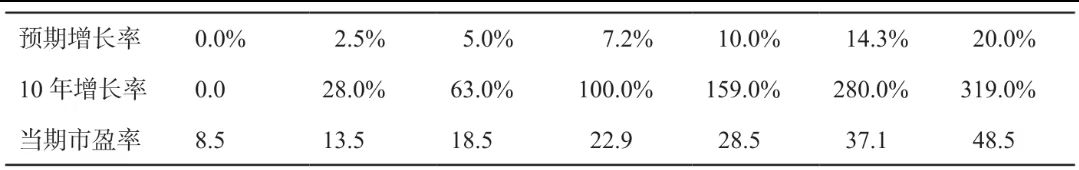
\includegraphics[width=\linewidth ,totalheight=0.95\textheight , keepaspectratio]{年度利润乘数.jpg}
\caption{根据简化的公式以及预期增长率计算出的年度利润乘数}
\end{figure}


根据我们的公式,很容易进行相反的计算,以确定当期市场价格所预期的增长率。

施乐公司32.4\%的内在年增长率,与通用汽车非常微弱的(2.8\%)增长率之间的差异,的确非常引人注目。其部分原因在于,股市认为,通用汽车1963年的利润(有史以来最大的一笔公司利润)难以实现,并且充其量也不会有太大的突破。另一方面,施乐的市盈率很好地代表了人们的投机热情:关注公司的巨大成就,而且期望将来的成就会更大。

道琼斯工业平均指数5.1\%的内在或预期增长率,要高于1951~1953年和1961~1963年期间3.4\%的实际(复合)年增长率。


我们要给出如下忠告:如果我们希望高成长股的增长率实际得以实现的话,那么预期增长率的估价必须相对保守。事实上,根据算术,如果假设一个企业将来可以按8\%或更高的速度无限期增长的话,那么其价值将趋于无穷大,且其股价无论多高也不过分。在这些情况下,估价者实际的行为是在其计算中引入安全边际(marginof safety)这一概念——类似于工程师在构造方面的规定一样。基于这种情况,即便实际的增长率结果大大低于预测结果,购买股票也能达到自己的目标(1963年,预期的总体年回报率为7.5\%)。当然,如果增长率实际得以实现,投资者必然会获取一笔可观的额外回报。事实上,没有办法估算出高成长企业(比如预期年增长率为8\%)的价值:分析师既不能实际估算出当期利润的恰当乘数,也不能估算出未来利润的预期乘数。

后来的事实证明,施乐和IBM公司的实际增长率,非常迫近于我们公式中所认为的高增长率。正如刚才所解释的,这个不错的结果,最终使得两者的股价大幅上升。道琼斯工业平均指数本身的增长,也接近于1963年市场收盘价的预测结果。但是,5\%这一较温和的增长率,并不会导致像施乐和IBM公司那样的数学难题。结果证明,23\%的价格上升(持续到1970年年底),再加上28\%的总股息回报,将使得公式中的总体年收益率大约达到7.5\%。就其他4家公司而言,我们只能说,它们的增长没有达到1963年的价格预期,而且其行市也没有道琼斯工业平均指数上涨得快。请注意:这里仅仅是为了进行说明而已——因为在证券分析中,必然涉及对大多数企业未来增长率的预测。读者不要错误地认为此类预测非常可靠,或者反过来认为未来价格将随着预测结果的实现、被超过或未达到而发生相应的变化。

应该指出的是,基于未来预期结果的“科学的”(或者说至少合理可靠的)股票估价,都必须考虑到未来的利率状况。如果所假设的利率更高一些,那么既定的预期收益或股息的现值就会小一些。这种假设始终很难可靠地做出,而且最近的长期利率大幅度波动,使得这种预测近乎武断。因此我们仍然使用上面的一个老方法,这只是因为没有更合理的新方法。

\subsection{行业分析}
由于企业的总体前景会对市场价格的确立产生重大影响,因此证券分析师自然会极大地关注行业及行业中单个企业的经济状况。这方面的研究非常细致。有时,这些研究会在重要因素方面获得一些宝贵的见解——此类因素将在未来发挥作用,但目前的市场并没有明显觉察到这一点。这方面得出的足够可靠的结论,有助于做出稳健的投资决策。

然而,我们自身观察后认为,面向投资者的大多数行业研究的实际价值并不是太大。所发掘出的材料一般都是公众非常熟悉的,而且已经对市场价格产生了重要的影响。很难发现某经纪公司会以一系列令人信服的事实告诉人们,某个受欢迎的行业即将崩溃,或者是某个不受欢迎的行业即将出现繁荣。华尔街对较远的未来的判断非常糟糕,这必然使得它的研究中的重要内容(对各个行业利润变化过程的预测)也很糟糕。

然而,我们不得不承认,近几年技术在迅速和广泛发展,这对证券分析师的态度和工作产生了重大影响。与以往相比,今后10年内一般企业的发展与否都将更大程度上依赖于新产品和新的生产流程,这使得分析师有机会事先进行研究和评估。因此,分析师的实际工作将有一个很好的前景——通过实地考察,通过与研究人员面对面的交流,以及通过分析师自身广泛的技术研究。如果投资结论主要来自于对未来的判断,而得不到目前明显的价值支持,这就存在着风险。然而,如果过分拘泥于以实际结果严格计算出的价值范围,同样也有可能存在着风险。投资者无法做到两者兼得。投资者可以发挥想象来对巨额利润做出判断,以便从可靠判断中获得回报,但是这种情况下,他必须承担错误计算有可能带来的任何巨大风险;投资者也可以保守些,拒绝向未经证实的可能结果支付太多的费用,然而,这种情况下,他必须准备将来为所放弃的绝佳机会而后悔。

\subsection{两步评估过程}
现在让我们暂时回到本书前面提到过的普通股估价或评估的问题。对此问题的大量思考使得我们认为,采用完全不同的做法,可能比现在通行的做法好得多。我们建议分析师首先搞清楚,我们所说的“以往业绩的价值”,完全取决于过去的记录。这将反映股票的价值状况(绝对状况,或者是道琼斯工业平均指数或标准普尔综合指数的百分比)——如果假设其以往的相关业绩将在未来持续下去的话。(这也包含了如下假设:其相关的增长率,比如过去7年的增长率,在随后的7年中也将保持不变。)这一过程可以按部就班进行:使用一个公式,计算出以过去的盈利能力、稳定性、增长率以及目前财务状况等数据为基础的各个权重;分析的第二步要考虑,完全以以往业绩为基础的价值,应该根据未来预期的新情况进行多大程度的修正。

这种方法对高级和初级分析师而言是有区别的:(1)高级分析师要确定可以应用于所有公司的一般化公式,以确定以往业绩的价值。(2)初级分析师要以十分简单的方式,计算出特定公司的这些因素的价值。(3)随后,高级分析师将决定,公司的业绩(绝对的或相对的)可能会在多大程度上偏离以往的记录,以及应该对价值进行多大的调整以反映这种预期变化。最好的结果是,高级分析师的报告中,既反映了初始价值,也反映了修正后的价值,以及价值调整的理由。

这种工作值得人们去做吗?我们的答案是肯定的,但我们的理由对读者来说似乎有点不太可信。我们不知道,对一般的工业企业(无论大小)而言,这样估算出的价值是否足够可靠。在下一章,我们将以美国铝业公司为例子来说明这项工作面对的难题。然而,对于这种普通股而言,只能采用这种方法。为什么?首先,许多证券分析师的日常工作就包含了对当期或预期价值的估算。我们所提出的方法,应该是对如今人们通常使用的方法的改进。其次,使用这种方法的分析师能够获得有用的经验和见解。第三,由于这类工作能够带来大量有价值的记录(医药领域很久以来一直如此),因此,这会促使更好的方法产生,并使人们能很好地了解其能力和局限性。公用事业股可以很好地证明,这种方法将在重要领域具有实际的价值。最终,聪明的分析师将使自己的工作限于下列行业群体:其未来似乎可以合理地做出预测;或者是以往业绩的价值相对于当期价格的安全边际很大,因此他可以对未来的变化做出推测,正如他在挑选十分稳妥的优先证券时那样。

在随后的章节中,我们将把这种方法应用于具体的例子。然而,这仅仅只是为了做出说明。如果读者对这项内容感兴趣的话,就应该进行系统和深入的研究,以便自己最终有能力做出证券投资决策。


\section{第11章点评}
\subsection{确定未来的价格}
哪些因素决定你购买股票时愿意支付的价格?是什么使得一家公司的价值达到其利润的10倍,而另一家公司的价值达到其利润的20倍?你如何保证自己不会因明显乐观的未来转变为一场噩梦而支付过大的代价?

格雷厄姆认为,有5种因素具有决定性的作用。他将其归纳为:

\begin{itemize}
\item 企业“总体的长期前景”
\item 企业管理层的水平
\item 企业的财务实力和资本结构
\item 企业的股息记录
\item 企业当期的股息支付率
\end{itemize}

让我们根据如今的市场来分析这些因素。

长期前景。如今,聪明的投资者首先要做的是,从公司网站或EDGAR数据库中下载至少5年的年度财务报告(10-K表),然后对这些财务报告进行梳理,收集证据,回答两个决定性的问题。这个企业增长的原因是什么?企业现在(以及将来)的利润来自何方?需要注意的问题包括:

\begin{itemize}
\item 企业是一个“连环并购者”。平均一年内有2~3起以上的并购,则预示着有可能出现麻烦。毕竟,如果某企业自身都认为应该购买其他企业的股份,而不愿从事自己的投资,那么,你为何不根据这一线索,也去观察一下其他企业?核实一下该企业以往的并购记录,注意食欲过盛的企业——它们吞下大企业后,最终只是又将其吐出来。朗讯、美泰、桂格麦片和泰克国际等企业,就曾经因吐出被并购的企业而遭受了惨痛的损失。其他一些企业因为以前并购价过高,而需要长期进行资产冲销或会计减记。对未来的业务而言,这是一个不祥之兆。
\item 企业是一位OPM成瘾者,通过借债或出售股份来抬升“他人资金”(Other People's Money,OPM)的总量。在年度财务报告的现金流量表中,这些慷慨注入的他人资金被称为“来自于融资业务的现金”。这些资金使得一家有问题的企业似乎正在成长,即使其基础业务并不能带来足够的现金——正如电信企业Global Crossing和世界通信不久前发生的情况一样。
\item 企业不太灵活,其大多数的收入都来自于某一个(或某几个)客户。1999年10月,光纤制造商Sycamore网络公司首次向公众发售了股份。招股说明书表明,该公司整个1 100万美元的收入,全部来自于威廉姆斯通信公司。交易商们乐观地估计,Sycamore的股票价值为150亿美元。不幸的是,只过了两年,威廉姆斯通信公司就破产了。尽管Sycamore公司挑选了其他客户,但其股票在2000~2002年期间损失了97\%。
\end{itemize}


当你研究企业的增长和利润的来源时,请同时关注有利和不利的因素。有利的迹象包括如下几项。

\begin{itemize}
\item 企业有宽广的“防御工事”或竞争优势。与城堡一样,有些企业很容易受到竞争对手的攻击,而另外一些企业则几乎是坚不可摧的。几种因素可以增强企业的防御能力:强有力的品牌形象(想一想Harley Davidson,其购买者会将该企业的标识物刺刻在他们的身上);对市场的垄断或近乎垄断;规模经济,即有能力廉价地提供大量商品或服务(想一想吉列公司,它能够廉价生产出几十亿只刀片);特有的无形资产(看一看可口可乐,其秘密的饮料配方没有任何有形价值,但却能吸引住宝贵的顾客);无法被替代(许多企业都不得不使用电力,因此,公用事业公司不可能在短期内被取代)。
\item 企业是一位长跑运动员,而不是一位短跑运动员。通过查看收益表,你会发现在前10年内,企业的收入和净利润是否在持续平稳地增长。《金融分析师杂志》上最近的一篇文章证实了其他的研究结果(以及许多投资者的惨痛经历):增长最快的企业,一般都会因发展过快而突然停止。从长远看,10\%的税前(或6\%~7\%的税后)利润增长是可持续的。然而,许多企业自己所确定的15\%的快速增长只是一个幻想。更高的增长率(或者说1~2年内的突然急速增长)必然会减缓下来,这就好比一个没有经验的马拉松运动员:试图以100米冲刺的方式来跑完全程。
\item 企业勤于播种和收获。无论企业的产品有多好,品牌有多强大,它都必须花一部分资金来拓展新的业务。尽管研发支出并不是当前增长的源泉,但很有可能是今后增长的源泉,尤其是当事实已经证明企业过去的振兴来自于新的思路和设备时。不同行业和不同企业的平均研发预算是不一样的。2002年,宝洁公司花在研发上的资金大约为其净销售额的4\%;而3M公司和强生公司在这方面的支出,分别为6.5\%和10.9\%。从长远来看,没有任何研发支出的企业,至少会与支出过大的企业一样脆弱。
\item 管理层的品质和行为。企业的高管应该言行一致。查阅以往的年度报告,核实管理者做出过哪些预测,以及他们是否达到了目标。管理者应该诚恳承认自己的失误,并承担相应的责任,而不应该拿“总体经济”“不确定因素”和“需求不足”等通用的理由作为替罪羊。查清企业董事会主席讲话的语气和内容是否前后一致,或者说是否随着最近的华尔街潮流而波动。(尤其要关注,在像1999年这样的繁荣年份,生产水泥或内衣的企业高管,是否突然宣布自己“成为软件革命的先行者”?)
\end{itemize}


这些问题有助于你确定企业管理者的行为是否符合企业所有者的利益:

\begin{itemize}
\item 他们是否在为自己谋求最大利益?

向自己的CEO支付1亿美元年薪的企业,最好能说出足够的理由。或许,他发现并独家拥有了青春泉(Fountain of Youth,传说饮此泉水能治百病,恢复青春;早期西班牙探险家曾在美洲和西印度群岛寻觅此泉——译者注)?或者他与外星人谈判达成协议,由地球上的这家公司单独向外星人提供全部供给?否则,这种可恶的巨额薪酬只是表明企业由管理者控制,并且是在为管理者谋利益。

如果企业对内部人员的股票期权进行重新定价(或者是“重新发售”或“进行交易”),就应该远离这样的企业。经过这种突然的逆转,企业会取消现有雇员和高管手中(一般都是没有价值的)股票期权,然后以新的有利价格的股票期权来取代它们。如果股票期权的价值永远不会下降为零,而且其潜在利润始终是无限的,它怎能激励高管管理好企业的资产呢?任何成熟的企业,如果像一些高科技企业那样对期权进行重新定价,这种行为都是不光彩的。购买此类企业的股票的投资者是自投罗网。

通过查看年度报告中关于股票期权的法定注释,你能够看到“期权溢价”有多大。比如AOL时代华纳公司在其年度报告的开头称,截至2002年12月31日,公司拥有45亿份普通股。但是,报告边缘的注释表明,该公司曾经发行的股票期权不低于6.57亿份。因此,公司未来的盈利将被另外15\%以上的股份去分享。当你估算企业未来的价值时,应该考虑股票期权有可能使新的股份大量增加。

通过EDGAR数据库中“表4”的内容,可以看到企业的高管和董事是否在购买和出售股份。企业内部人员有合理的理由(资产分散化,换更大的房子,办理离婚等)去出售股份,但是多次大规模出售则是一个明显的警示信号。当你在不断地买入而管理者却在不断卖出时,他不可能成为你理想的合作伙伴。
\item 企业高管是管理者还是推销员?

企业高管应该将大部分时间用于管理企业的内部事务,而不应该向公众投资者推销自己的企业。许多情况下,CEO们都会抱怨自己的股价被低估了(无论股价有多高)。他们忘记了格雷厄姆一贯坚持的观点:企业的管理者应该力求防止自己的股价被过分低估或高估。与此同时,太多的首席财务官会提供“利润指导”,即对企业的季度盈利做出猜测。一些企业喜欢到处张扬,不断发布新闻,吹嘘一些暂时的、微不足道的或假想的“机会”。

少数企业(包括可口可乐、吉列和USA Interactive)开始向华尔街的短视思维“直接说不”了。企业中这些少数的勇敢者正在提供越来越多关于其当期预算和长期计划的详情,而拒绝对今后90天内的情况做出推测。(想知道某企业如何与其股东进行平等和诚恳的沟通,请进入EDGAR数据库,查看华盛顿国际快递公司提供的8-K表,它会定期公布该机构与股东之间精彩的问答内容。)

最后,搞清楚企业的会计业务是为了使其财务结果透明化,还是模糊化。如果“一次性的”费用不断发生,“异常”项目经常出现而成为普通项目,那么EBITDA(Earnings Before Interest,Taxes,Depreciation and Amortization的缩写,指的是未计入利息、税费、折旧和摊销的净利润——译者注)这样的字首组合词要比净收益更重要,或者说,“预测的”利润被用来掩盖了实际亏损。这就可以说明该企业还没有学会如何把股东的长远利益放在首要地位。

\item 财务实力和资本结构。对优良企业最基本的定义是:所获取的资金要多于所消耗的资金。优秀的管理者不断寻找各种方法,以将这些资金投入生产活动。从长远来看,满足这一定义的企业,几乎必然要出现价值的增长,而无论股市如何表现。

在企业的年度报告中,首先阅读其现金流量表,以查明过去10年内,其营业现金流量是否在稳步增长。然后再进一步往下看。巴菲特的一个流行概念就是所有者收益,即净收益加上摊销和折旧,再减去正常的资本支出。这就正如Davis Selected Advisors公司的资产组合管理者克里斯托弗·戴维斯所说的:“如果你完全拥有这家企业,年底时你的口袋里将会有多少现金?”由于考虑到了摊销和折旧这样一些不影响企业现金余额的会计项目,因此,所有者收益是比所报告的净收益更好的一个计量指标。为了对所有者收益的定义进行改进,你还应该从所报告的净收益中减去下列项目:

\begin{itemize}
\item 分配股票期权的所有成本——这使得一部分收益从现有股东手中转移到新的所有者手中。
\item 任何“异常的”“一次性的”或“特殊的”费用。
\item 任何来自于企业养老基金的“收入”。
\end{itemize}
如果过去10年中,每股所有者收益总体上一直按高于6\%或7\%的速度增长,这就说明该企业有稳定的现金流,而且增长前景很好。

按下来,看企业的资本结构。从资产负债表中查看企业有多少债务(包括优先股在内)。一般而言,长期债务应该低于总资本的50\%。根据财务报告表中的注释,确定长期债务是固定利率(利息支出不变),还是浮动利率(利息支出会变化,如果利率上升,支出会增加)。

从年度报告中,查看所公布的“利润与固定费用之比”。亚马逊网络公司2002年的年度报告公布的结果表明,该公司的利润比其利息成本少1.45亿美元。将来,亚马逊公司要么需要从其业务中赚更多的钱,要么需要以更低的利率借到资金。否则,该企业最终将不能被其股东所有,而是要被其债券持有者所有——如果这些债券持有者不能获得应得的利息,他们就可以对亚马逊的资产行使求偿权。(公平地讲,亚马逊2002年的利润与固定费用之比比两年前的情况好多了,当时偿还债务的利润缺口为11亿美元。)

下面是关于股息和股票政策的几点看法(更多的内容,请参见第19章)。

\begin{itemize}
\item 最主要的是,企业要证明,如果不支付股息,股东的结果会更好。无论市场好与坏,如果企业都始终能够在竞争中获胜,那么这就清楚地表明,管理者最有利地利用了资金。可是,如果业务在下降,或者股票的表现不如其竞争对手,那么就说明企业的管理者和董事是在通过拒付股息而滥用资金。
\item 不断进行股票分割的企业(以及不断通过新闻发布而吹嘘股票分割的企业),是把投资者当成了傻瓜。就像约吉·贝拉一样(他要把比萨饼分成4份,其原因在于“我想,我吃不了8份。”),喜欢股票分割的股东并不理解这一点。价格为50美元的两份股票,并不比价格为100美元的一份股票更值钱。通过股票分割来推销自己股票的管理者,是在鼓励和纵容投资大众最邪恶的原始本能,因此,在把资金托付给此类表面热心的操纵者之前,聪明的投资者要三思而后行。

\item 企业应该在股价便宜时回购其股份,而不应该在股价处于或接近于最高位时回购股份。遗憾的是,近几年常见的现象是,企业在股价被高估时回购其股份。没有比这种浪费企业资金的行为更可笑的了,因为这种操作的真实意图是使企业高管能够以“提升股东价值”为名义出售自己的股票期权,以获取上百万美元的丰厚回报。
\end{itemize}

事实上,众多的实际证据表明,声称“提升股东价值”的管理者极少能这样去做。与普通的生活一样,在投资领域,最终的获胜者通常是实干家,而不是空谈家。

\end{itemize}


\section{对每股收益的思考}
这一章,我们从针对投资者的两条建议开始,这两条建议的含义必然是相互矛盾的。第一条建议是:不要过于看重某一年的收益。第二条是:如果你确实关注短期收益,请当心每股收益数据中存在的陷阱。如果我们严格遵守第一条告诫,那么第二条告诫就没有必要存在。但是,我们不能指望大多数股东根据长期记录和长远前景做出所有普通股决策。在金融领域,季度数据尤其是年度数据会受到极大关注,而且这种关注必然会对投资者的思维产生影响。在这一领域,需要对投资者进行一些教育,因为这里充斥着误导性的东西。

...


所有这一切都会使我们的读者感到困惑和乏味,但这就是我们所面临的情况。公司会计经常是需要慎重对待的;证券分析会非常复杂;股票估价只有在非常罕见的情况下,才是真正可靠的。对大多数投资者而言,最好的方法或许是,确保自己购买的证券物有所值,并且这样保持下去。

\subsection{平均利润的使用}
以前,分析师和投资者会高度关注以往相当长时间(通常为7~10年)内的平均利润。这个“平均数”有助于缓和商业周期经常带来的利润波动,因此,人们认为它比最后一年的结果更能反映企业的盈利能力。这种平均法的一个重要优势在于,它几乎可以解决所有特殊费用和利益的问题。这些费用和利益应该包含在平均利润中。因为,毫无疑问,这些损益中的大多数都代表了企业的一部分营运历史。就美国铝业而言,如果我们这样做的话,那么其1961~1970年(10年)间的每股平均收益为3.62美元,1964~1970年(7年)间的每股平均收益为4.62美元。如果将此数据与同期的利润增长率和稳定性结合起来使用,就可以看到该公司以往业绩的实际状况。

\subsection{过去增长率的计算}
正确考虑企业的增长记录是很重要的。当增长率很高的时候,企业近期的利润将会大大超出7年或10年的平均数,因此分析师可能会认为,这些长期数据缺乏相关性。但情况并不一定如此。利润既可以用平均值来衡量,也可以用最新的数据来衡量。我们建议,增长率本身的计算,可以采用把近3年平均数与10年前的相应数据进行对比的做法。(这样,当存在“特殊费用或利益”的问题时,可以采用某种折衷的方法。)


...



\section{第12章点评}
\subsection{数字游戏}
过去几年内,企业及会计师的行为已经显得十分不得体,如果格雷厄姆在世的话,也会大跌眼镜。在以大量的股票期权获取薪酬之后,企业的高管们意识到,仅仅借助于企业利润在几年之内的增长,他们就能够变得异常富有。大量的企业违背了会计精神(即便没有违背其字面含义):将财务报告弄得无法理解;掩饰不利结果;隐藏费用;凭空捏造利润,等等。让我们来看一看其中的一些不光彩行为。

\subsection{预计利润}
或许最流行的一个会计骗局就是“预计”(pro forma)利润的大量使用。在华尔街有一个古老的说法:任何坏主意的出发点都是好的。预计利润的公布也不例外。预计利润的本意是通过对短期偏差和“不经常发生的”事件进行调整,以便更为真实地反映利润的长期增长。比如,所发布的预计利润可能会让人们看到,如果某公司刚刚收购的另一家企业已经成为该公司的成员满12个月的话,那么该公司在过去一年中的利润将是多少?

...

简而言之,预计利润使得企业可以向人们展示:如果没有失误,它们将会做得多么好。作为一个聪明的投资者,在预计利润这一点上,你惟一能做的就是忽略它们。

\subsection{急于确认收入}
2000年,电信行业的巨头奎斯特国际通信公司(Qwest Communications International Inc.)看上去实力很强大。尽管当年的股市下跌了9\%以上,但该公司的股票下降幅度还不到5\%。

但是,在奎斯特的财务报告中有一个奇怪的小发现。1999年年底,当电话簿刚一出版,奎斯特就决定确认来自电话簿的收益。但是,登载过黄页广告的客户都知道,许多企业是采用按月支付的方式来偿付这些广告费用的。真是莫名其妙!私下“改变会计准则”的做法,使其1999年的税后净利润增加了2.4亿美元,相当于奎斯特当年全部收益的五分之一。

正如冰山一角,急于确认利润经常是存在重大危险的迹象,奎斯特的情况正是如此。2003年年初,在查看了以前的财务报表之后,该公司承认:提前确认了出售设备的利润;不恰当地记录了外部服务的费用;不恰当地将成本当成了资本资产,而没有将其当成费用;不恰当地将资产置换当成了直接的销售。所有这一切加起来,使得奎斯特2000和2001年的销售收入被高估了22亿美元,其中包括前面所说的“改变会计原则”(此时已经纠正过来了)带来的8 000万美元的收入。

\subsection{违反资本方面的规定}
20世纪90年代末,Global Crossing公司雄心勃勃。这家设在百慕大的公司,正在建设所谓的“首条一体化的全球光纤网络”。网络长达10万英里以上,主要分布在全球的洋底。连接全球之后,Global Crossing将向其他通信公司出售有线网络的使用权。仅1998年一年,Global Crossing在建设光纤网络方面就花费了6亿多美元。同一年,几乎三分之一的建设预算从收入中扣除了——以所谓的“出售设施的成本”的名义。如果没有这1.78亿美元的费用,该公司应该可以报告近8 200万美元的净利润——但是,所报告的净亏损达9 600万美元。

接下来的一年,Global Crossing在1999年年度报告的一个不起眼的注释中称“开始使用服务合约会计”。该公司不再将大多数的建设成本作为费用,从出售网络设施的收入中直接扣除。相反,现在大部分的建设成本将不再看做营运费用,而是看做资本支出。因此,这将使该公司的资产总额增加,而不是使其净利润下降。

不可思议!魔杖一挥,Global Crossing的“财产和设备”资产就增加了5.75亿美元,而其销售成本只增加了3.5亿美元,尽管该公司在漫无边际地花钱。

资本支出是企业管理者增强企业实力的一个重要工具。但是,灵活的会计原则使得管理者可以通过将正常营运费用转变为资本资产来夸大其报告利润。从Global Crossing这个案例中可以看到,聪明的投资者一定要搞清楚公司资本化的来源及理由。

\subsection{一个关于存货的故事}
与许多半导体芯片制造商一样,美光科技公司(Micron Technology,Inc.)的销售额在2000年后开始下滑。事实上,需求的急剧下降给美光以沉重打击,以至于它不得不开始下调其存货的价值,因为客户显然不会按美光的报价来购买这些产品。在2001年5月结束的那个季度,美光将存货的价值记录砍去了2.61亿美元。大多数投资者并没有把这项减记看成正常的或经常性的营运成本,而是看成了一个特殊事件。

可是,我们来看随后发生的情况。在随后的6个财务季度内,美光公司都做了存货减记。美光公司存货价值的下降是一次性的事件,还是一种常态呢?理性思考的人可以对这件事做出区分,但有一点是明确的:聪明的投资者必须始终小心那些不断发生的“一次性”成本。

\subsection{退休金方面的问题}
2001年,SBC通信公司(它拥有Cingular Wireless、Pac Tel和新英格兰南部电话公司的权益)获得了72亿美元的净利润。在电信业能力过剩的情况下,这是一个耀眼的业绩。但是,这部分利润并非完全来自于SBC的业务,其中的14亿美元(占公司净收益的13\%)来自于SBC的退休金计划。

由于SBC退休计划中的资金多于员工未来估计要获得的退休金,因此,该公司将这一差额当做当期收入。产生盈余的原因很简单:2001年,SBC将退休计划投资的预期回报从8.5\%提高到了9.5\%,从而降低了如今需要划拨的退休金。

关于更加乐观的预期,SBC的解释是:“2001年结束时每个3年期之内,我们实际的10年投资回报率都超过了10\%。”换句话讲,我们过去的回报率很高,因此,我们可以假设未来的回报率也很高。然而,这不仅不符合最基本的逻辑标准,而且还面对着如下的情况:利率即将降到历史最低水平,这将降低退休金组合中债券的未来收益。

实际上,巴菲特的伯克希尔-哈撒韦公司在同一年,将其退休金资产的预期收益率从8.3\%降低到了6.5\%,SBC认为其退休基金经理的业绩,能大大超过全球最优秀的投资者,你认为这现实吗?不太可能成为现实:2001年,伯克希尔-哈撒韦退休基金的收益为9.8\%,而SBC的退休基金则亏损了6.9\%。

在此,聪明的投资者要考虑这样几个重要的问题:“退休金的净收益”会比公司的净利润高出5\%吗?(如果是这样的话,当将来这些退休金收益不存在时,你还会对该公司的其他收益感到满意吗?)这里所假设的“退休金计划资产的长期回报率”符合情理吗?(截至2003年,任何高于6.5\%的收益率都是不合情理的,而更高的收益只不过是幻想而已。)

\subsection{给投资者的几点忠告}
下面的几点建议,可以使你避免购买有会计隐患的股票。

从后往前看。当你研究某企业的财务报告时,从最后一页开始,慢慢地往前阅读。凡是企业不愿意你看到的东西都放在后面,这就是你应该首先查看后面的原因。

查看说明。在未阅读年度财务报告的有关说明之前,决不能去购买股票。通常,在“重要会计政策总结”这一栏中,有一个关键性的说明会告诉你,该公司如何确认收入,如何记录存货,如何对待分期付款或合约销售,如何分摊营销成本,以及如何记录其他一些主要的业务。在其他注释中,注意查看关于债务、股票期权、客户贷款、损失准备以及其他“风险因素”的信息,因为这些因素将吞食掉大量的利润。会使你的敏感神经抽动的其他一些技术术语有“资本化的”“递延的”和“重组的”,等等。像“开始”“改变”和“然而”等简单明了的英文词汇,则预示着公司已经改变了自己的会计行为。这些词语中的任何一个并不意味着你不应该购买该公司的股票,但它们表明,你应该做进一步的调查。一定要把这些注释内容至少与一个密切竞争企业财务报告中的注释进行比较,以查看你所关注的企业的会计师有多么激进。

阅读更多的内容。如果你是一个积极投资者,愿意在证券组合中花大量的时间和精力,那么你就应该更多地了解财务报告的内容。为了尽可能防止被变化多端的收益表所误导,这是惟一的办法。下面的3本书包含了大量适时的相关例子:Martin Fridson和Fernando Alvarez合著的《财务报表分析》、Charles Mulford和Eugene Comiskey合著的《财务数字游戏》,以及Howard Schilit所著的《财务骗术》。



\section{第13章点评}
\subsection{E字打头的企业}
让我们像格雷厄姆那样对四种股票进行对比。我们使用的是1999年12月31日财务报告中的数据——这一时间可以使我们看到一些股市有史以来出现的最严重的极端价格。

爱默生电气公司(股票交易代码:EMR)成立于1890年,是格雷厄姆当初所举出的四家企业中惟一的幸存者。该公司提供种类繁多的产品,其中包括电动工具、空调设备和电动马达。

EMC公司(股票交易代码:EMC)的历史可以追溯到1979年。它的业务是使得一些公司可以在计算机网络上自动储存电子信息。

华盛顿康捷国际物流公司(股票交易代码:EXPD)于1979年在西雅图成立。它帮助发货人组织并追踪货物在全球的运送。

Exodus通信公司(股票交易代码:EXDS)向公司类客户提供和管理网站,同时还有其他一些互联网服务。它于1998年3月首次向公众发售股份。

下表概括了1999年年底这几家公司的股价、业绩和估值情况。

\begin{figure}[H]
\centering
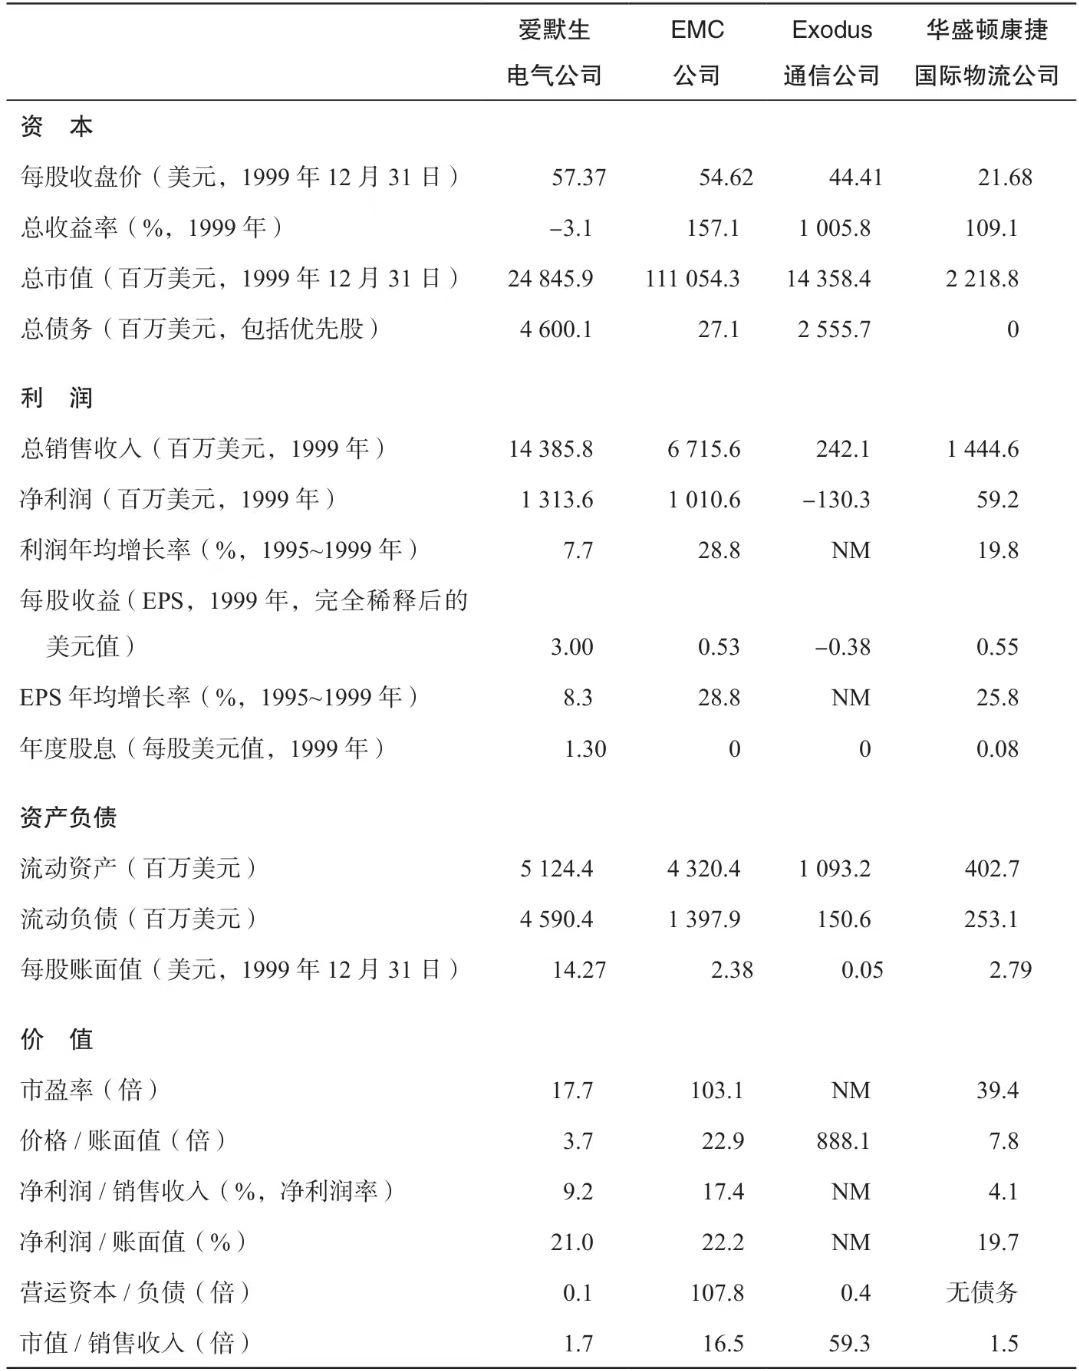
\includegraphics[width=\linewidth ,totalheight=0.95\textheight , keepaspectratio]{对E字打头的四家公司的估值.jpg}
\caption{对E字打头的四家公司的估值}
\end{figure}


说明:所有数据都考虑到了后来的股票分割。负债、销售收入和利润都以财务年度为单位。市值:普通股总价值。NM:无意义。

\subsection{电气企业的表现并不令人振奋}
在格雷厄姆列举的四种股票中,爱默生电气的价格最为昂贵。但在我们新的一组企业中,爱默生的价格是最便宜的。由于属于旧经济产业,20世纪90年代末,爱默生失去了吸引力。(在互联网时代,谁还会去关注爱默生产的重型干湿真空吸尘器呢?)公司的股价陷入了长期低迷。1998年和1999年,爱默生的股票累计滞后于标准普尔500指数49.7个百分点,这是一个令人沮丧的不良业绩。

然而,这是爱默生公司股票的情况。爱默生公司的业务情况如何呢?1999年,爱默生出售了价值达144亿美元的商品和服务,比前一年增加了近10亿美元。爱默生从这些收入中赚取了13亿美元的净利润,比1998年增长了6.9\%。前5年中,每股收益以平均8.3\%的速度强劲增长。爱默生的每股股息增长1倍多,达到了1.3美元;账面值从每股6.69美元增加到了14.27美元。根据价值线公司提供的数据,整个20世纪90年代,爱默生的净利润率和资本回报率这两个反映其业务效率的关键性指标一直都很强劲,分别为9\%和18\%。此外,爱默生的利润连续增长达42年之久,股息连续增长长达43年之久,这是美国企业稳步增长时间最长的一个例子。1999年年底时,爱默生的股价为其每股净收益的17.7倍。与其生产的电动工具一样,爱默生从不耀眼,但却是可以信赖的——而且没有出现过过热的现象。

\subsection{EMC公司能够快速增长吗}
EMC公司是20世纪90年代股票表现最佳的一家公司——股价上升(或飞涨)速度超过了810倍。如果在1990年年初,你有EMC公司1万美元的投资,那么1999年年底,你的投资价值将上涨到810万美元以上。仅1999年一年,EMC的股票回报率就达到了157.1\%——这超过了爱默生从1992年到1999年8年间的总回报。EMC从未支付过股息,相反,它将所有的利润“用于公司的持续发展”。按12月31日54.625美元的股价来看,EMC股票的交易价格为该公司全年报告利润的103倍——几乎是爱默生股票估价水平的6倍。

EMC的业务状况如何呢?1999年业务收入增长了24\%,达到了67亿美元。其每股收益从一年前的61美分,激增到了1999年的92美分,增长达51\%。在截至1999年的5年内,EMC的利润以28.8\%的年增长率急速增长。而且,由于每个人都认为电子商务浪潮会持续下去,因此其未来前景更加光明。整个1999年,EMC的负责人不断地预测,2001年的业务收入将达到100亿美元——比1998年增加54亿美元。这要求年增长率达到23\%。对于如此大规模的一家公司而言,这将是一个惊人的增长速度。然而,华尔街的分析师及大多数投资者都确信,EMC能够做到。毕竟,在过去的5年中,EMC的销售收入增加了一倍多,其净利润超过了两倍。

然而,根据价值线公司提供的数据,从1995年到1999年,EMC的净利润率从19\%下滑到了17.4\%,其资本回报率从26.8\%降到了21\%。虽然还有较高的盈利,但EMC已经在走下坡路。1999年10月,EMC并购了Data General公司,从而使得自己当年的业务收入大约增加了11亿美元。直接将Data General所带来的收入扣除之后,我们可以看到,EMC已有的业务量,从1998年的54亿美元只增加到了1999年的56亿美元,上涨幅度只有3.6\%。换句话讲,EMC的实际增长率几乎为零——即便在计算机“千年虫”恐慌使得许多公司在新技术方面的花费创下历史纪录的情况下。

\subsection{货运公司的简单情况}
与EMC不同,康捷国际物流公司从未出现过飞速增长。尽管20世纪90年代该企业的股价年增长率为30\%,但其中大部分增长来自于最后一年——1999年股票的回报率快速增长了109.1\%。此前的一年,康捷的股票仅上涨了9.5\%,落后于标准普尔500指数19个百分点。

公司的业务状况如何?实际上,康捷的增长非常迅速:从1995年开始,其业务收入年增长率达19.8\%;到1999年结束时,业务量达14亿美元,这一时期几乎增加了两倍。每股收益的年增长率达25.8\%,股息年增长率高达27\%。康捷公司没有长期债务,其营运资本自1995年后几乎增加了一倍。根据价值线公司提供的数据,康捷的每股账面值上升了129\%,其资本回报率达21\%(上升了三分之一以上)。

无论以任何标准来衡量,康捷都是一家优秀的企业。但是,这家小型货运公司(设在西雅图,而许多业务位于亚洲)在华尔街却几乎没有什么名气。其股份只有32\%被机构投资者持有。事实上,康捷公司只有8 500名股东。1999年倍增之后,该公司的股价为当年净利润的39倍。这并不太低,但是却大大低于EMC令人头晕的估价。

\subsection{应许之地?}
截至1999年年底,Exodus通信公司似乎将自己的股东直接带入了福地。1999年的股价激增了1 005.8\%,足以使得1月1日的1万美元投资,在12月31日变成11万美元。华尔街著名的网络股分析师(包括美林证券的重量级分析师亨利·布洛杰特在内),都预测该公司的股票在随后一年中还将上涨25\%~125\%。

在网络股交易者(他们从Exodus的股票中获得了大量的收益)看来,最为有利的是,1999年该公司的股票进行了三次2比1的分割。在2比1的股票分割中,公司的股份数将增加一倍,股价将下降一半。因此股东拥有的股份最终为原来的两倍,而每股价格只有以前的一半。这有什么了不起的?假如你给我一个10美分的硬币,而我返还给你两个5美分的硬币,并问“你感到现在更富有了吗?”你可能会说我是一个傻瓜,或者说,我误认为你是一个傻瓜。可是,在1999年互联网股市的狂热中,网络交易商的行为似乎就是认为,两个5分的硬币要比一个10分的硬币更值钱。事实上,仅仅按2比1进行股票分割的消息,就能使其股价立即上涨20\%或更多。

为什么会这样?因为拥有更多的股份会使人们感到更加富有。某人在1月份买的Exodus公司的100股,经过4月份的分割后就变成了200股;8月份的200股又变成了400股;12月份400股又变成了800股。使这些人感到振奋的是,起初他们只有100股,但是现在却增加了700股。他们感觉似乎是“发现了财路”,而从不考虑每一次分割,都将使股价下降一半。1999年12月,一位购买了Exodus股票的得意洋洋的股民(其网名为“给我一美元”)兴奋地在网上发帖子称:“我将把这些股票保留到我80岁为止,(因为)随后经过上百次的股票分割之后,我将要成为CEO了。”

Exodus 的业务状况如何?格雷厄姆将不会去碰该公司的股票。Exodus 的业务收入呈爆炸式增长——从1998年的5 270万美元,增加到了1999年的2.421亿美元。但是,1999年的这些业务导致了1.303亿美元的亏损,几乎为前一年亏损额的两倍。Exodus 总共有26亿美元的债务,而且急需资金,因此仅在12月它就借了9.71亿美元。根据Exodus 的年度报告,这笔新的借款将使它下一年的利息支出增加5 000多万美元。1999年年初,该公司的现金为1.56亿美元,即使通过新的融资又筹集了13亿美元,但这一年结束时的现金余额只有10亿美元——这意味着,1999年,公司的业务吃掉了4亿多美元现金。这种公司如何去偿还自己的债务呢?

但是,网络股交易者显然只关注股票的上涨幅度及速度,而不会去关注公司是否稳健。网名为“Launch\_{}Pad1999”的一位交易者夸耀道:“这只股票将继续无止境地上涨。”
Launch\_{}Pad荒谬的预测——何谓“无止境”?——正好提醒人们要记住格雷厄姆经典的告诫。格雷厄姆告诉我们:

\begin{quote}
“如今的投资者是如此关注对未来的预期,以至于已经事先付出了巨大的代价。这样,即使他大力进行细心的研究,得出的预测结果成为现实,也有可能仍然无法获利。如果预测的结果没有完全实现,他实际上将面临着严重的短期亏损甚至是永久性的亏损。”
\end{quote}


\subsection{四家公司的结果如何}
这四种股票1999年之后的表现如何?

2000年,爱默生电气又获得了40.7\%的收益。尽管其股票在2001和2002年均出现了亏损,但2002年结束时的价格,比1999年最后的价格下降了不到4\%。

2000年,EMC的股价也上涨了,其盈利达21.7\%。然而,2001年,其股价降了79.4\%,2002年又降了54.3\%。这使得股价比1999年年底的水平低88\%。预测2001年的业务收入为100亿美元,其结果如何?这一年EMC最终的业务收入只有71亿美元(并且有5.08亿美元的净亏损)。

与此同时,对于康捷国际来说,似乎根本没有出现熊市,其股价在2000年增长了22.9\%,2001年增长了6.5\%,2002年又增长了15.1\%——2002年结束时的股价几乎比1999年年底的高出51\%。

Exodus的股价2000年下降了55\%,2001年下降了99.8\%。2001年9月26日,Exodus依照破产保护法第11章提出了破产申请。该公司的大多数资产被英国的电信巨头Cable \& Wireless收购了。未能将自己的股东带入应许之地,相反,Exodus将他们流放到了荒野之中。2003年年初,Exodus股票的最后交易价为每股1美分。


\section{防御型投资者的股票选择}
现在,我们要将证券分析方法应用于更广泛的领域。因为我们已经概括地向两类投资者推荐了应该采纳的投资策略,因此,现在我们要介绍,为了实施这些策略该如何进行证券分析。采纳我们建议的防御型投资者,只会购买高等级的债券以及多样化的优质普通股。他们必须以实际标准来判断自己购买的普通股价格没有严重高估。

在确定分散化的组合时,防御型投资者有两种可供选择的方法:类似道琼斯的证券组合以及定量检验的证券组合。按照第一种方法,他实际上要获得这些优质股的横向分析样本,其中既包括一些增长较快的公司(其股票的市盈率非常高),也包括一些不太受欢迎和股价不太高的企业。要做到这一点,最简单的办法或许就是,以相同的数额购买道琼斯工业平均指数中的所有30种股票。在平均指数为900的情况下,如果每种股票买入10股的话,总共将要花费大约16 000美元。根据以往的业绩记录,购买几种具有代表性的投资基金的股份,投资者将来能获得大致与以前相同的结果。

按照第二种选择,在每次购买证券时,都要使用一套标准,以确保:(1)公司过去的业绩以及当期的财务状况达到某一最低的标准;(2)利润和资产与股价之比达到某一最低的数量。在前一章的结尾,我们列出了选择特定股票时的7项质量和数量标准。下面我们逐一进行介绍。

\begin{enumerate}
\item 适当的企业规模

我们所提出的各项最低限额要求都是主观武断的,尤其在企业规模方面。这么做是要把小公司排除在外,因为小公司更容易发生变化,尤其是在工业领域。(此类企业中经常会有很好的机会,但我们认为,它们并不适合于防御型投资者的需要。)让我们给出大致的数额:就工业企业而言,年销售额不低于1亿美元;就公用事业企业而言,总资产不低于5 000万美元。
\item 足够强劲的财务状况

就工业企业而言,流动资产至少应该是流动负债的两倍——所谓的二比一的流动比。同时,长期债务不应该超过流动资产净额,即“营运资本”。就公用事业企业而言,负债不应该超过股权(账面值)的两倍。
\item 利润的稳定性

过去10年中,普通股每年都有一定的利润。


\item 股息记录

至少有20年连续支付股息的记录。

\item 利润增长

过去10年内,每股收益的增长至少要达到三分之一(期初和期末使用三年平均数)。
\item 适度的市盈率

当期股价不应该高于过去3年平均利润的15倍。
\item 适度的股价资产比

当期股价不应该超过最后报告的资产账面值的1.5倍。然而,当市盈率低于15倍时,资产乘数可以相应的更高一些。根据经验法则,我们建议,市盈率与价格账面值之比的乘积不应该超过22.5。(这相当于15倍的市盈率,乘以1.5倍的账面值。同时,也可以是这样的股票:9倍的市盈率和2.5倍的资产价值等等。)


\end{enumerate}



总结:这些要求是专门针对防御型投资者的需求和特征而给出的。它们以两种相反的方式,将绝大多数的普通股排除在证券组合之外。一方面,它们要排除下列公司:(1)规模太小;(2)财务实力相对较弱;(3)过去10年中有赤字记录;(4)没有在长时间内连续支付股息的历史。在目前的金融条件下,所有最严格的检测标准都是判断财务实力的指标。近几年,许多大企业和实力曾经雄厚的企业,都出现了流动比的弱化或债务的扩张。


我们最后的两个标准,可以从相反的方向进行排除:要求每一美元股价拥有更多的利润和更多资产,从而排除流行的股票。这决不是经济分析师标准的看法;事实上,大多数分析师坚持认为,即使保守型投资者也可以以较高的价格购买优秀企业的股票。在上文中我们阐述了相反的观点。这种观点主要建立在缺乏适当安全性的基础之上,即股票的价值主要依赖于未来利润的不断增长。读者自己必须对这个重要的问题做出决定——权衡这两种相互对立的观点。

然而,我们还要考虑过去10年内适度增长这一要求。如果没有这一项要求,一般的公司都会出现退步,至少以每一美元投资资本的利润来衡量是如此。防御型投资者没有理由把此类公司包括在内,但是,如果股价足够低则是非常好的投资机会。

我们建议的15倍的最大市盈率,很有可能使得一般证券组合的平均市盈率大约达到12~13倍。请注意,1972年2月,美国电话电报公司股票的售价是其3年(和当期)利润的11倍;而加州标准石油公司的股价,低于其最新利润的10倍。我们的基本建议是,所购股票组合的总体利润与价格之比(市盈率的倒数),至少应该与当期高等级债券的利率一样高。这就意味着,不高于13.3倍的市盈率,相当于收益率为7.5\%的AA级债券。

...





\subsection{防御型投资者的选择}
每一位投资者,都希望自己挑选的股票表现更好或前景更佳。因此,读者会问,如果自己选择一位有能力的顾问或证券分析师,是否能指望获得真正具有优势的投资组合呢?“毕竟,”他可能会说,“你所指出的这些规则都非常的简单和容易。受过严格训练的分析师,应该能够使用其技巧和方法,来对道琼斯这样平淡无奇的组合做出极大的改进。否则分析师所做的统计、计算和权威判断等所有这一切有什么用呢?”

作为一个实际检验,设想我们要求100位证券分析师,在道琼斯工业平均指数中挑选出“最好的”5种股票,以便在1970年年底时买入。很少有人会做一样的选择,而且,所选的5种股票也会不一样。

稍加思考,这并不令人奇怪。根本原因在于,每种优质股票的当期价格都很好地反映了财务记录中重要因素的影响,以及人们对其未来前景的总体看法。因此,任何分析师的观点(认为某种股票优于其他股票的观点),都必定在很大程度上源于其个人的偏好和预期,或者说是来自于这样一个事实:在分析过程中,他更加重视某一组因素,而不太重视另外的因素。如果所有的分析师都认为某一特定的股票要优于其他的股票,那么该股票的价格将迅速上升,从而抵消它以前所具有的各种优势。

我们称当期价格反映了已知事实和未来预期,是为了强调市场估价的双重基础。与这两类价值因素相对应的,是证券分析的两种基本方法。的确,每一位有能力的分析师,都会关注未来,而不会关注过去;而且,他能意识到,自己工作的好与坏,取决于将要发生的结果,而不是已经发生的结果。然而,未来本身可以通过两种不同的方法来实现——我们可以将其称为预测法(或项目法)和保护法。

重视预测的那些人,会努力去准确预测未来几年公司会有多大的成就,尤其是利润是否会出现显著和持续的增长,这些结论来自于对行业供求等因素(交易额、价格和成本)的研究;也可以根据过去的业务增长来简单地推测未来。如果这些权威们确信,长期前景非常有利,他们几乎总是会建议人们购买该股票,而不太去关注股票的售价。比如,人们对航空运输股一般就持有这种态度。这种态度持续了多年,尽管1946年后,航空股的表现经常令人失望。在本书的导言中,我们已经讨论过这一行业的强势股价与其较差盈利之间的不一致。

相反,重视保护的那些人,总是重点关注研究时的股票价格。他们的努力主要在于,确保自己获得的现值足够大于市场价格——这一差额可以吸纳未来不利因素造成的影响。因此,一般而言,他们不必热心关注公司的长期前景,而只需要有理由相信,企业将会持续经营下去。

第一种方法(即预测法)也可称为定性法,因为它强调的是未来前景、管理状况,以及其他一些不可计量但却很重要的定性因素。第二种方法(即保护法)可以称为定量法或统计法,因为它强调的是股票售价与利润、资产和股息等因素之间存在的可计量的关系。实际上,定量法是人们把证券分析中债券和优先股投资选择的方法扩展到普通股领域而产生的。

就我们自身的态度和本职工作而言,我们始终致力于定量法。从一开始,我们就要确保我们的投资能够以具体而可靠的形式获得丰厚的价值。我们不愿意以未来的前景和承诺,来补偿眼下价值的不足。这决不是投资权威们普遍持有的观点。实际上,大多数人可能都持有如下观点:未来前景、管理层的水平、其他无形资产及“人力因素”,要比对以往记录、资产负债表和所有其他枯燥无味的数据进行研究后得出的结论重要得多。

因此,从根本上讲,“最优”股票的选择存在极大的争议。我们建议防御型投资者不要去管这个问题。防御型投资者要更重视股票的分散化,而不是个股的选择。顺便要指出的是,人们普遍接受的分散化观点(至少在一定程度上)否认了选择性方面的优势。如果能够正确地挑选出最佳的股票,那么分散化就只能带来不利后果。然而,在我们向防御型投资者所建议的普通股选择四大原则范围之内,人们的偏好有着相当大的自由空间。从最不利的角度来看,纵容这种偏好应该不会有坏处,除此之外,它还有可能使结果得到改善。随着技术进步对企业长期结果的影响越来越重要,投资者不得不考虑这方面的因素。与其他方面一样,这里投资者也必须在忽视与过分重视之间找到一个折衷点。




\section{第14章点评}
\subsection{行动起来}
你该如何应对股票选择这种细致的工作?格雷厄姆建议,防御型投资者可以“直截了当地”购买道琼斯工业平均指数中的每一种股票。如今,防御型投资者能够做得更好:购买整个股票市场指数基金,该基金实际上持有每一种值得拥有的股票。低成本的指数基金,是专门针对小额股票投资的最佳工具。任何想获得更优结果的行为,都将要付出更多的劳动(并且会导致更大的风险和更高的成本),而这对真正的防御型投资者来说是不恰当的。

自己通过研究而挑选股票是不必要的。对大多数人而言,这甚至是不明智的。然而,一些防御型投资者的确会通过挑选个股,来获得娱乐和享受智力挑战。而且,如果你成功经历了熊市,并且仍然能从挑选股票中获得乐趣,那么,格雷厄姆和我所说的任何话,都将不能阻止你这么去做。这种情况下,不要把整个股票市场指数基金作为你的全部证券组合,而是将其作为你的证券组合的基础。一旦你拥有了这个基础,就可以围绕它来做一些自己选择股票的试验了。将购买股票的资金的90\%投入指数基金,而将剩余的10\%用于自己挑选股票。只有在建立了这个稳固的核心之后,你才能去做一些探索。


\subsection{不断的检验}
让我们简要地更新格雷厄姆的股票选择标准。

适度的规模 如今,“为了排除小企业”,大多数防御型投资者应该完全避免购买市值总额不到20亿美元的股票。2003年年初,在标准普尔500指数中,有437家这样的公司可供选择。

然而,与格雷厄姆时代不同,如今的防御型投资者,能够购买专门从事小企业股票交易的共同基金,从而方便地拥有小企业的股份。需要再次指出的是,先锋小企业指数基金(Vanguard Small-Cap Index)是人们的首选,当然,像Ariel、T.Rowe Price、Royce和Third Avenue这样的活跃型基金,也可以按合理的成本购买到。

强有力的财务状况 根据市场战略家加布里斯和摩根士丹利的拉瑟斯提供的信息,在2003年年初,标准普尔500指数中,大约有120家企业能够满足格雷厄姆提出的2:1的流动比标准。由于它们的流动资产至少为流动负债的两倍,因此,这些大规模的流动资本缓冲(一般)能帮助它们度过难关。

...

利润的稳定性 根据摩根士丹利提供的数据,从1993年到2002年,标准普尔500指数的所有公司中,有86\%的公司每年的利润都为正。因此,格雷厄姆所坚持的“过去10年内每年的普通股都有一定的利润”是一个合理的标准——这足以排除经常亏损的企业,但却又不会使你的选择严格局限于不太现实的少数样本企业。

股息记录 根据标准普尔提供的数据,2003年年初,该指数中有354家公司(占总数的71\%)支付了股息。多达225家公司连续支付股息至少长达20年。而且,根据标准普尔提供的信息,该指数中,有57家公司至少在连续25年内提高了自己的股息。虽然这并不能保证将来会永远如此,但这却是一个令人欣慰的迹象。

利润的增长 在截止于2002年的10年间,标准普尔500指数中,有多少家公司的每股收益增长达到了格雷厄姆所要求的“至少三分之一”?(我们将计算出每家公司在1991~1993年的平均利润,然后再看2000~2002的平均利润是否至少增加了33\%。)根据摩托根士丹利提供的信息,标准普尔500股中,有264家公司达到了这一标准。在此,格雷厄姆似乎设定了一个非常低的门槛:10年内33\%的累积增长,意味着年均增长率还不到3\%。如果要求每股收益至少累积增长50\%(年均增长4\%),就不是太保守了。2003年年初,标准普尔500指数中满足这一标准的公司不少于245家,因此,防御型投资者有大量的选择余地。(如果将累积增长门槛调高一倍而达到100\%,即相当于7\%的年均增长率,那么,满足标准的公司为198家。)

适度的市盈率 格雷厄姆建议,只购买当期价格不超过过去3年平均利润15倍的股票。难以置信的是,如今华尔街通行的做法是以当期股价除以所谓的“下一年利润”来对股票进行估价。这就是有时候人们所称的“远期市盈率”。但是,以已知的当期价格除以未知的未来利润来获取市盈率的方法是不明智的。货币经理德曼告诉我们,从长远看,华尔街“一致”采用的利润预测方法中,有59\%会出现很大的偏差——比实际的报告利润低估或高估至少15\%。根据短视的预言家对下一年的预测结果来进行投资,这种行为的风险就好比在射箭锦标赛上,自愿为有资格参赛的盲人举起靶子一样。相反,投资者应该利用格雷厄姆的方法(以当期股价除以过去三年的平均利润),亲自计算股票的市盈率。

2003年年初,标准普尔500指数中,有多少种股票的价格没有超过其2000~2002年平均利润的15倍?根据摩托根士丹利提供的信息,一共有185家公司达到了格雷厄姆的标准。

适度的价格与账面值之比 格雷厄姆建议,“股价与资产之比”(价格与账面值之比)不得高于1.5。最近几年,公司价值中有越来越多的部分来自于特许权、品牌、专利权和商标等无形资产。由于这些因素(以及并购所获取的商誉)不符合账面值的标准定义,因此,如今大多数公司的价格账面值要高于格雷厄姆时代的情况。根据摩托根士丹利提供的信息,标准普尔500指数中有123家公司(占四分之一)的价格与账面值之比要低于1.5,总共有273家公司(占该指数的55\%)的价格与账面值之比在2.5以内。

格雷厄姆建议,将市盈率乘以价格与账面值之比后,观察其结果是否小于22.5。那么,这方面的情况如何呢?根据摩托根士丹利提供的数据,2003年年初,标准普尔500股中,至少有142种股票符合这一标准,其中包括Dana 公司、电子数据系统公司、太阳计算机系统公司和华盛顿互助银行。因此,格雷厄姆的“混合乘数”,仍然可以作为合理定价股票的初选工具。

\section{积极型投资者的股票选择}
在前面一章中,我们以各类符合条件的证券为基础,介绍了普通股选择的方法。只要能达到一定程度的分散化,防御型投资者就可以根据自身或投资顾问的偏好,从这些类别的证券中自由构建证券组合。我们在证券选择方面主要强调如何进行各种排除,一方面,建议人们不要去购买质量明显较差的股票;另一方面,建议人们不要去购买价格太高,以致投机风险太大的高等级股票。本章针对的是积极投资者。我们要分析个体选择的可能性及方法,这些方法有可能带来高于整体平均水平的利润。

能够成功做到这一点的可能性有多大?委婉地说,如果在这一点上不首先表达一些重要的保留意见,我们就显得不太直率。乍一看,成功选择的例子似乎是不言而喻的。获得一般的结果——比如说,相当于道琼斯工业平均数的业绩——并不需要任何特殊才能,所需要做的只不过是建立一个等同于或类似于那30种优质股票的证券组合而已。这样,毫无疑问,只要利用一定的技巧(学习、经验和天性所带来的技巧),就有可能获得大大优于道琼斯工业平均指数的结果。

然而,大量明显的证据表明,要做到这一点是十分困难的,即便试图这样做的那些人拥有很高的水平。这些证据表现在众多投资公司或“基金公司”多年业务的记录中,这些基金中的大多数都具有很大的规模,它们在该领域拥有最佳的金融和证券分析服务,同时还拥有所有其他应有的研究部门。它们的业务费支出占其庞大资本的比重,平均每年大约为0.5\%,或者更低一些。这些成本本身并不是一个小数,但是与1951~1960年这10年间普通股大约15\%的总体年回报率相比,或者甚至是与1961~1970年6\%的回报率相比,都显得并不太高。少数具有超级选择能力的人应该很容易克服这种费用障碍,并且给基金股东带来极其可观的净收益。

然而,从总体上看,在相当长的年份内,整个普通股基金并没有像标准普尔500股平均指数或整个市场那样获得很好的回报。...


正如我们在第9章所指出的,这些数据的比较绝没有否认投资基金作为一类金融机构所起到的作用。因为,它们的确使所有投资公众都有可能获得近似于平均水平的普通股投资收益。由于各种各样的原因,大多数公众投资者在自己所选择的普通股方面的投资,都没有基金投资的业绩好。但是,在客观的观察者看来,基金的业绩未能超过一般水平的事实正好证明,要想获得超出一般水平的成就并非一件易事,而实际上是非常困难的。

为什么会出现这种现象?我们认为有两种不同的解释,这两种解释都能部分说明问题。第一种解释认为存在如下可能:股市的当期价格的确既包含了关于公司过去和当期业绩的所有重要事实,同时也包含了对公司未来的所有合理预期。如果是这样的话,那么之后市场发生的各种变化(这些变化经常会非常剧烈),一定是由于无法准确预见的新进展和可能性所导致的结果。这将使得股价变动完全成为偶然的和随机的。如果上面所说的果真如此,那么证券分析师的工作(无论他多么聪明,以及研究得多么深入)将大体上是无效的。因为从本质上讲,他是在力求对不可预测的东西做出预测。

证券分析师人数的众多,或许在导致这一结果方面起到了重要的作用。由于有成百甚至上千的专家正在研究影响某种重要股票价值的各种因素,因此,人们自然会认为,股票的当期价格很好地反映了专家对其价值的共识。那些偏好某种股票的人,是出于个人的偏好或乐观看法,而这种偏好和乐观看法既有可能是正确的,也有可能是错误的。

我们经常会把华尔街诸多证券分析师的工作,与复式桥牌锦标赛上桥牌大师们的表现进行类比。前者力求挑选出“最有可能成功的”股票,后者力求为每一手牌获取最高的分数。两类人中,都只有极少数的才能达到目标。由于所有桥牌手都具有大致相同的专业水平,因此获胜很有可能是取决于各种“机会”,而不是高超的技能。在华尔街,这种平衡过程来自于职业联合会。借助于该联合会,一些想法和发现能够非常轻松地被参加各种聚会的业内人士分享。这就好比在桥牌锦标赛上,各位专家相互观察对方的姿态,并且对所打出的每一手牌进行辩论一样。

第二种解释完全不同。或许,许多证券分析师的能力,是因为解决股票选择问题的基本方法存在着缺陷而受到了阻碍。他们寻求的是增长前景最好的产业,而且这些公司在该行业中拥有最佳的管理层和其他优势。这就意味着,他们将购买这些产业和这些公司的股票,无论其股价有多高;同样,他们将避开前景不太看好的产业和公司的股票,无论其股价有多低。这种做法的正确性只会发生在下列条件下:这些优秀企业的利润必将在未来无限期地高速增长下去。因为只有这样,企业的价值从理论上讲才是无限的。同样,如果前景不看好的企业在无助中走向灭亡,那么,分析师认为其股价再低也没有吸引力的观点才是正确的。

公司的实际情况是完全相反的。只有极少数公司能够显示出长时间内连续的高增长。同时,少数大公司也会令人意外地遭受最终的消亡。大多数企业相对的历史地位都是会发生变化的——有上升,也有下降。有些企业会不断经历“从贫穷,到富有,再到贫穷”这样的周期性变化(这是过去曾经用在钢铁行业方面的一种一致的说法);另一些企业会随着管理水平的恶化或改进而发生重大变化。

上述研究结果在多大程度上适合于积极投资者(他们愿意通过个人选择来获得更好的结果)?这一研究首先表明,积极投资者所从事的是一项艰难而且还有可能是不切实际的工作。无论多么聪明,知识多么渊博,本书的读者都不太可能在证券选择方面比本国的分析师做得更好。但是,如果从标准的选择分析的角度来看,股市上真的有很大一部分股票经常受到歧视,或者是完全被忽视,那么,聪明的投资者就可以从其相应的价值低估中获利。

但是,要做到这一点,他就必须遵循与华尔街通行的做法不一样的特殊方法,因为那些已被人们所接受的方法,似乎并不能带来每个人都想要的结果。如果聪明的人都在股市中从事职业投资,但是还存在既稳妥却又比较不受欢迎的方法,那么,这将是一件十分奇怪的事。然而,我们自己的职业和声誉,一直是以这种不可能的事实为基础的。

...


\subsection{二类企业}
接下来要考察和选择的是二类企业。这类企业的情况看上去不错,以往的业绩也令人满意,但对公众却缺乏吸引力。...在此,我们将尝试一种新的方法,并且详细阐述此类方法在股票选择中的使用。我们的目的有两个。...《股票指南》...


\subsection{根据《股票指南》进行筛选}
假设想找出股票便宜的明显证据,我们首先想到的是,价格相对于近期利润而言较低。让我们对1970年年底市盈率不高于9倍的股票进行初步的排列。...

这一类股票看上去价格都不太高,其中有10种股票的每股售价在10美元以内。

因此,让我们将其他一些标准应用于我们所挑选出的股票。这些标准非常类似于我们向防御型投资者所提出的建议,只不过没有那么严格。我们建议:

1.财务状况:(a)流动资产与流动负债之比至少达到1.5;(b)(对工业企业而言)债务占净流动资产的比例不高于110\%。

2.盈利稳定:在《股票指南》近5年的数据中没有出现过赤字。

3.股息记录:目前有一些股息支付。

4.利润增长:去年的利润高于1966年的利润。

5.股价:不高于有形资产净值的120\%。

...最终将有大约150家公司满足我们全部的6项选择标准。这样,积极投资者就可以根据自己的判断(偏好和倾向)进行第三次选择。比如从这个范围较广的名单中选出20\%。

...



\section{第15章点评}
\subsection{练习,练习,再练习}
Mutual Series基金的创始人马克斯·海涅(Max Heine)喜欢这样一句话:“通往耶路撒冷的路不止一条。”这位股票大师的意思是,他自己以价值为核心的股票挑选方法,并非是成功的投资者惟一可使用的方法。在本章点评中,我们将介绍如今一些优秀的货币经理在挑选股票时所使用的几种方法。

然而,首先要再次指出的是,个股选择对大多数投资者而言是不必要的,尽管可以这样去做。大多数专业人士在股票选择方面都做得很差,这也就意味着业余人士不可能做得更好。绝大多数试图挑选股票的人都发现,他们做的并没有想象的那么好。极为幸运的人早就发现了这一点,而不太幸运的人则要花几年时间才能懂得这一点。少数投资者擅长挑选自己的股票,其他人要通过别人的帮助(最好是通过指数基金)才能做得更好。

格雷厄姆建议投资者首先要练习,正如优秀的运动员和音乐家在每次实际表演之前的练习和排练一样。他建议,投资者首先花一年的时间去跟踪和挑选股票,但并不是真的去投资购买。...

在实际投资之前对你的技巧进行检验,你即使犯错也不会造成任何实际损失,并且还能避免形成频繁交易的习惯,将自己的方法与那些优秀货币经理的方法进行比较,了解哪些方法是有效的。最为有利的是,跟踪你所有股票挑选的结果,将使你不会忘记,你的一些预感最终被证明是错误的。这将迫使你既向成功者学习,也从失败者身上吸取教训。一年之后,将你的结果与标准普尔500指数基金进行对比,看情况如何。如果你不喜欢这项试验,或者你的选择结果很差,这也没有什么损害,这说明个股选择的做法不适合你。如果这样,就去挑选一家指数基金,不要在股票选择上浪费时间了。

如果你很喜欢这项试验,并且获得了足够高的回报,就可以逐步建立股票组合了。但是,这一股票组合在你的整个证券组合中的比重不能超过10\%(将其余资金投入指数基金),而且要记住,如果你对此不再感兴趣,或者你的回报变得太差的话,你可以随时停下来。



\subsection{老板是谁}
最后要讲的是,大多数优秀的专业投资者都希望公司由这样的人来管理:“不只是经理人,而是像所有者那样进行思考。”(Oakmark公司的尼格伦如是说。)这方面有两个简单的标准:公司的财务报告易于理解,还是模棱两可?“一次性的”、“异常的”和“特殊的”费用是事实上如此,还是令人不愉快地经常出现?

Longleaf公司的梅森·霍金斯寻找的是这样的公司经理:他们是“良好的合伙人”——他们开诚布公地讨论问题,他们对当期和未来现金流的分配有明确的计划,而且他们拥有该公司大量的股份(最好是通过现金购买的,而不是通过派送期权获得的)。可是,“如果企业管理层大谈股价而少谈业务,”Torray基金的罗伯特·托雷告诫说,“我们是不感兴趣的。”Davis基金公司的戴维斯希望企业将股票期权的发行额控制在现有股份大约3\%的范围之内。

先锋Primecap基金的霍华德·肖跟踪的是,“公司第一年所说的是什么,第二年发生的情况又是什么。我们不仅要了解管理层是否对股东诚实,而且还要了解他们自己是否说到做到。”(如果某公司的老板在业务混乱时坚持认为一切都令人满意,请保持警觉。)如今,即使只拥有少数的几股,人们也可以定期参加公司的股东大会。想知道股东大会召开的时间,可以电话联系公司总部的公共关系部门,或者访问公司的网站。

FPA资本基金的罗德里格斯会查看公司年度报告的背面——这里列有各个业务部门负责人的名单。如果在新的CEO任期内的头一年或两年中更换了许多名字,这可能是一个好兆头:说明他正在淘汰不称职的人。可是,如果此后还是不断更换人名的话,这种调整就有可能转变成混乱。


\subsection{从每股收益转向投资资本回报}
由于股票期权派送以及会计盈利和扣除等因素的影响,近几年的每股净收益或每股收益(EPS)已经被扭曲了。想了解公司经营活动中所使用的资本带来的真实利润,就需要从每股收益转向投资资本回报(ROIC)。Davis基金的克里斯托弗·戴维斯将ROIC以下列公式来定义:

ROIC=所有者收益÷投资资本

\begin{verbatim}
公式中的所有者收益等于:
营业利润
加上 折旧
加上 商誉的摊销
减去 联邦所得税(按公司的平均所得支付)
减去 股票期权的成本
减去 “维持”(或实际的)资本支出
减去 不可持续的养老金回报所带来的任何收益
(2003年,任何高于6.5\%的回报都是不可持续的)
\end{verbatim}


\begin{verbatim}
公式中的投资资本等于:
资产总额
减去 现金(以及短期投资和非生息的流动负债)
加上 过去降低投资资本的会计扣除
\end{verbatim}

ROIC的优点在于,它在扣除所有合理费用之后,反映了公司从其经营活动中所获利润,以及公司在利用股东资金获取回报方面有多大的效率。ROIC只达到10\%就很有吸引力了;即使6\%或7\%也会有吸引力,如果该公司有一个好的品牌、目标明确的管理层,或者只是遇到了暂时的困难。

\subsection{看清道路}
还有其他更多通往耶路撒冷的道路。

一些优秀的证券组合经理(比如Dreman价值管理公司的戴维·德尔门和Third Avenue基金公司的马丁·惠特曼)都把目光集中于资产、利润或现金流的乘数非常低的公司。也有人(比如,Royce基金的查尔斯·罗伊斯和富达低价股基金的乔尔·蒂林哈斯特)追逐的是价值被低估的小公司。想简要了解如今最受尊敬的投资者巴菲特是如何选择公司的,请参见下面的专栏内容。

有一种方法会有所帮助:看哪一位优秀的职业货币经理与你持有相同的股票。如果经常会出现一两个这样的人,请访问这些基金公司的网站,并下载其最新的报告。通过查看这些投资者还拥有其他的股票种类,你能更多地了解这些股票的共同点。通过阅读经理的评论,你会知道如何去改进自己的方法。

无论他们使用什么样的技巧来挑选股票,成功的投资专家都有两个共同点:首先,他们遵守既定的约束,并一贯坚持自己的行为,拒绝改变自己的方法,即便这种方法已不再流行;其次,他们大量思考的是做什么以及如何去做,而很少去关注市场情况如何。


\subsection{巴菲特的做法}
格雷厄姆最优秀的学生沃伦·巴菲特已经成为了全球最成功的投资者,其做法是在格雷厄姆想法的基础上设计出新的窍门。巴菲特及合伙人查尔斯·门格(Charles Munger)把格雷厄姆的“安全性”和远离市场的观点,与自己强调未来增长的创新做法结合起来了。下面是对巴菲特方法的简要介绍。

他寻求的是“特许经营”的公司,该公司有很强的消费品牌,有很容易被人们理解的业务活动,有强有力的财务状况,以及有近乎于垄断的市场——比如H \& R Block 、吉列和华盛顿邮报等公司。巴菲特喜欢在公司丑闻、巨额亏损和其他坏消息似乌云飘过时迅速下手购买其股票——比如,1987年可口可乐公司推出的“新可乐”遭到惨败、公司股价崩盘后,他迅速买入了该公司的股票。他还喜欢公司的经理具备下列行为:制定并实现合理的目标;从自己内部而不是通过并购来拓展业务;明智地进行资本分配;不给自己派送上百万美元的股票期权奖金。巴菲特坚持认为,利润的增长应该是稳步和持久的,这样,公司未来的价值会比今天更大。

在自己的年度报告(参见www.berkshirehathaway.com)中,巴菲特完全袒露了自己的思想。或许,没有哪一位投资者(包括格雷厄姆在内)会公开透露更多关于自己投资方法的信息,或公开发表如此通俗易懂的文章。(巴菲特有一句经典名言:“当声誉卓越的管理层经营一家企业而搞得一团糟的时候,人们心目中将只会留下企业的形象。”)每一位聪明的投资人都可以(和应该)通过阅读这位大师自己的语言来获得更多的知识。



\section{可转换证券及认股权证}
最近几年,在优先债权融资领域,可转换债券和优先股正在成为主导力量。与此同时,股票期权这种认股权证(可以按规定价格购买普通股的一种长期权证)已经越来越流行了。...

从总体上看,可转换证券比认股权更为重要,因此,我们将首先对前者进行讨论。从投资者的角度来看,有两个主要的方面需要考虑。首先,它们的投资机会和风险大小如何?其次,它们的存在会对相关普通股的价值产生怎样的影响?

人们认为,可转换证券对投资者和债券发行企业都具有特殊的优势。投资者既可以获得债券或优先股享有的优先保护,同时还有机会分享普通股急剧上升所带来的好处。证券发行者能够按适度的利息或优先股股息来筹集资本,而且,如果所预期的业务兴旺成为现实,发行者还可以将其转换成普通股,消除这部分优先债务。因此,交易双方都会感到非常满意。

显然,上述这段话一定有所夸大,因为你不可能仅仅通过一种巧妙的手段使交易双方都获得好处。在获取转换权的同时,投资者通常要在证券的质量或收益(或同时在两方面)做出一些重要的让步。反过来看,如果公司因为证券具有转换权而获得低成本资金的话,那么这是因为它同时放弃了普通股股东未来收益增长的一部分。关于这一话题,正反双方都有一些不明确的观点需要进一步探讨。可以得出的最稳妥的结论是:与其他任何形式的证券一样,可转换证券本身并不能保证这种证券一定具有吸引力——这个问题将取决于与单个证券相关的所有事实。

然而,我们的确知道,总体上讲,牛市后期发行的一类可转换证券必然不能得到满意的收益。(遗憾的是,过去大多数的可转换融资正是发生在这种乐观时期。)从时间选择本身来看,悲剧将不可避免,因为股市的大幅下跌,必然会使得人们对这种证券本身的基本安全性产生怀疑。作为对此类证券的说明,我们将保留本书第一版中使用过的、关于可转换优先股和一般的(不可转换)优先股相关价格行为的例子——这些证券于1946年发行,是1949年开始进入特殊时期之前的一个牛市期的最后一年。

对1967~1970年的情况很难做出比较,因为这几年几乎没有发行过新的不可转换证券。但是可以清楚地看到,从1967年12月到1970年12月,可转换优先股平均价格的下降幅度,大于普通股的整体下降幅度(普通股只下降了5\%)。同时,从1968年12月到1970年12月,可转换优先股的业绩似乎比以前发行的不可转换优先股的业绩差许多——这一点可以从表16-2中每种股票的20个样本反映出来。从这些比较中可以看出,作为优先证券的可转换证券的整体质量都比较差,而且它们所关联的普通股的业绩也比一般市场情况要差(投机猖獗时期除外)。当然,这些观点并不适合于所有的可转换证券。尤其在1968年和1969年,许多实力强大的公司为应对过于高昂的利率(即便最优级债券的利率也很高)发行了可转换证券。然而,值得注意的是,在20种股票构成的可转换优先股样本中,只有一种出现了上涨,并且有14种出现了严重下跌。


这些数据得出的结论,并不是说可转换证券本身比不可转换或“一般的”证券要差。同等条件下,结论正好相反。然而,我们可以清楚地看到,在实践中,其他条件不可能等同,而且可转换权的获得,经常(或许普遍地)会以丧失证券实际的投资质量为代价。

的确,可转换优先股比同一公司的普通股要更安全一些——也就是说,其本金最终亏损的风险要小一些。因此,购买新发行的可转换优先股,而不去购买相应的普通股的行为是符合逻辑的。然而,在大多数情况下,尽管最初按市场价购买普通股的行为是不明智的,但是,用可转换优先股来代表普通股的做法,并不足以使情况得到改善。此外,可转换优先股大多是由那些对普通股没有特殊兴趣或信心的人所购买的(也就是说,他们当时并没有想到要去购买这种普通股,而是被可转换优先股表面上的优先求偿权与接近于当期市场的转换权的完美结合吸引住了)。某些情况下,这种结合能很好地发挥作用,但统计数据似乎表明,它更有可能是一种陷阱。

在拥有可转换证券方面,大多数投资者都没有认识到一个特殊的问题。即使产生了利润,也有一个两难的选择。证券持有人是应该在小幅上涨后就卖掉呢,还是应该继续持有以等待更大的上涨?如果这种证券被赎回(当普通股大幅上涨时,经常会发生这种情况),那么持有者是应该将其卖掉,还是应该将其转换为普通股而继续保留下去呢?

让我们来看一个具体的例子。假设你花100美元购买了利率为6\%的债券,该债券可以按25美元的价格转换成股票——每1 000美元的债券可转换成40股。现在股价达到了30美元,从而债券的价值至少为120美元,且债券现在的售价为125美元。你可以出售或保留债券。如果你继续持有债券,希望价格上涨得更高,你面临的状况将十分类似于一个普通股股东,因为如果股价下跌,你的债券也将下跌。一个保守的投资者可能会说,价格高于125美元后,其头寸的投机性会太大,因此,他会将其出售,并赚取令人满意的25\%的利润。

眼下一切都令人满意。但让我们进一步探讨这个问题。许多情况下,当债券持有人按125美元价格出售时,普通股还在上涨,从而使得可转换债券的价格也在上涨,这样,过早出售债券的投资者就会感到心疼。下一次,他决定将债券持有到价格上升为150或200美元时为止。债券价格上涨为140美元,但他并没有将其出售。随后,市场崩盘,其债券价格滑落到80美元。这样,他又犯了一次错误。

除了这些错误判断所带来的精神痛苦(它们似乎是不可避免的)之外,在可转换债券的操作方面,还存在着真实的算术缺陷。人们也许认为,对许多持有者而言,采用严格一致的策略——利润达到25\%或30\%时将其出售——会获得很好的结果,但这只是利润的上限,而且只有表现良好的债券才能实现这一目标。可是,如果(正如事实所表明的)这些债券经常缺乏适当的标的证券,并且一般是在牛市后期发行和购买时,其中很大一部分将无法达到125美元的价格,而当市场发生逆转时,会不可避免地出现崩盘。所以,实践证明,可转换债券诱人的机遇只是一种幻觉,而且总体经验表明,这种交易既存在着巨大的利益,也完全有可能出现巨大的亏损(至少是暂时性的亏损)。

由于1950~1968年期间存在着一段相当长的牛市,因此,可转换债券在大约18年内总体上表现不错。但这只是意味着,绝大多数普通股的价格都出现了大幅上涨,所以大多数可转换债券也能分享这一价格上涨的好处。可转换债券投资的稳健性,只能通过它们在股市下跌时的业绩来判断——但事实证明,这种情况下它们的总体结果总是令人失望的。

...

因此,对于新发行的可转换债券,我们一般都是持怀疑态度的。与其他类似的观点一样,在此我们的意思是,投资者在购买可转换债券之前要三思而后行。经过此类排除性的考察之后,投资者可能会发现一些无法拒绝的特殊债券。当然,最理想的情况是同时具备下列条件:一种基础非常牢固的可转换债券,可以按照稍高于当期市场的价格转换成本身具有吸引力的普通股。时常会有一些新发行的债券符合这些要求。可是,从证券市场的性质来看,与新发行的债券相比,好像更有可能在一些已发行的债券(它们已经具备了更有利的地位)中找到这种机会。(如果一种新的债券真的实力很强,那它不太可能拥有好的转换权。)

...

\subsection{可转换证券对普通股地位的影响}
许多情况下,可转换证券的发行都与公司的兼并或新的收购相关。这种金融业务最显著的一个例子,或许就是NVF公司发行的近1亿美元利率为5\%的可转换债券(包括认股权证)——其目的是换取Sharon钢铁公司大多数的普通股。这一特殊交易将在下文进行探讨。通常,这种交易会导致每股普通股所报告的预计利润的增加;股价会随着所谓的更多利润而增长,同时,股价的增长还在于公司管理层已经证明它有能力、有信心为股东赚取更多的利润。但是存在着两种会带来抵消作用的因素,其中一种实际上被忽略了,另一种在乐观的市场也会完全被忽略。第一种因素是,随着新的转换权的不断增加,普通股当期和未来的利润实际上会被稀释。这种稀释作用可以计算出来:根据目前的利润和对其他一些数据的假设可以计算所有的可转换股票或债券实际进行转换后每股的调整利润。对大多数公司而言,所导致的每股数据的下降并不明显。但是,在这方面有很多例外,而且其危险在于,这种下降的幅度会迅速加大。迅速扩张的“综合性大企业”一直在玩弄可转换证券的花招。...


\subsection{从普通股向优先股的转变迹象}
10多年之前(比如1956年),普通股的收益要高于同一家公司的优先股。如果优先股的转换权接近于市场价值,情况尤其如此。现在总的情况正好相反。结果,大量可转换的优先股明显比相关的普通股更具有吸引力。通过将次级股份转变成优先证券,普通股的所有者并不会有什么损失,但却具有很大的获利优势。

比如,1970年年底,Studebaker-Worthington公司的情况就是一个典型的例子。该公司的普通股售价为57美元,而5美元的可转换优先股最终的价格达到了87.5美元。每一份优先股可以交换1.5份普通股(当时普通股的价格为85.5美元)。这表明,购买优先股与购买普通股的差价很小。然而,普通股支付的年股息额为1.20美元(每1.5股为1.80美元的股息),优先股每股获得的年股息为5美元。因此,最初不利的价格差,可能会在不到1年的时间里得到弥补;此后的一段时间内,优先股股息带来的回报会明显高于普通股。当然,最为重要的是,普通股股东从这种转变中所获取的优先地位。在价格较低的1968年以及1970年,优先股的售价比1.5份普通股要高出15个点。正是可转换权保证了优先股的售价不可能低于普通股组合。

\subsection{股票期权}
让我们开门见山吧。我们认为,最近兴起的股票期权近似于一种欺诈行为,是潜在的一种威胁,而且还有可能引发灾难。它们凭空捏造出了大量的美元“价值”。除了误导投机者和投资者之外,它们的存在没有任何理由。它们应该受到法律的禁止,或者至少应该被严格限制在公司资本总额的很小一部分范围之内。

为了与一般的历史和文学进行类比,我们建议读者去阅读《浮士德》(Faust)的部分内容(第2篇)——在这部分内容中,歌德描述了纸币的发明。作为华尔街历史上一个凶兆的先例,我们将谈到American \& Foreign Power公司的权证——1929年,这些权证的市场价值超过了10亿美元,尽管它们只出现在公司资产负债表的注释中。到了1932年,这10亿美元缩水成了800万美元,而在1952年,这些权证就从公司的资本结构中消失了——尽管公司尚未破产。

起初,股票期权这种权证时常是与债券有联系,而且通常都相当于部分转换权。它们在数量上并不重要,因此没有什么害处。与许多其他的金融舞弊行为一样,它们的使用在20世纪20年代末开始扩张,不过,此后的许多年内,它们退出了人们的视线。但它们势必会重新抬头,就像不想看见的东西一再出现一样。而且,从1967年开始,它们成为人们熟知的“融资工具”。实际上,新的不动产企业和大银行的附属机构,设计出了一种标准的筹资方法:出售相同数量的普通股和权证单位,以便按相同的价格购买额外的普通股。比如,1971年,CleveTrust Realty Investors公司以每单位20美元的价格,出售了250万份这种由普通股(或“受益股份”)和权证所构成的组合。

现在,让我们来看这种融资方案所真正涉及的内容。通常情况下,当公司董事会认为有必要以普通股来筹集资本时,普通股股东首先有权购买额外发行的股份。这种所谓的“优先认购权”是普通股所有权带来的一种价值——此外,还有获取股息的权利,分享公司成长的权利,以及投票选举董事的权利。为了获得额外的资本而单独发行权证的时候,这种行为将会带走普通股固有的一部分价值,并将其转移给独立的权证。以此类推,人们还可以发行单独获取股息的权证(期限有限或期限无限的),发行单独分享企业销售收入或资产清理收益的权证,或者是发行单独拥有股票投票权的权证。那么,为什么这些认股权证被当做初始资本结构的组成部分呢?就是因为,人们对金融业务不太熟悉。人们没有认识到,与没有权证时相比,权证的存在会使得普通股的价值下降。所以,与只有股票相比,股票与权证的组合通常会获得更好的市场价格。需要指出的是,在通常的公司报告中,每股收益的计算并没有(或一直没有)对已有权证的影响给予适当的考虑。当然,所造成的结果是夸大了利润与公司资本的市场价值之间的实际关系。

把权证的存在考虑在内的最简单和最好的方法,就是将其市场等值额加入到普通股资本中去,因而增加每股的“实际”市场价。如果出售优先证券的同时有大量的权证,那么,通常的调整方法就是假设出售股票的收入被用于偿还相关的债券或优先股。

...


公司本身通过设立这些权证能获得好处吗,即这些权证能确保公司在必要情况下获得额外的资本吗?根本不可能。一般情况下,公司根本不可能在权证到期之前要求其持有者行使其认购权。与此同时,如果公司想要筹集额外的股本,它就必须按通常的方式向股东发行股票——也就是说,要按稍低于市场的价格发行股票。在这项业务中,权证并不能提供什么帮助,它们只是会让情况变得更加复杂——不断要求公司对自己的认购价往下调整。我们要再次申明的是,除了制造出市场价值幻觉之外,发行大量的股票期权起不到什么作用。

撰写《浮士德》时,歌德所熟知的纸币就是法国发行的臭名昭著的指券(assignats)。人们曾经把这种纸币称做一项了不起的发明,但它们最终却失去了所有的价值。American \& Foreign Power公司10多亿美元的权证也是如此。这位诗人的有些话,同样能很好地适用于这样或那样的发明——比如下列对话(来自于Bayard Taylor的译文):

\begin{quotation}
浮士德:人们无法完全理解倾其所能的最高想象力。

靡非斯特(发明者):如果人们需要钱币的话,掮客们可以随时提供。

傻瓜(最后说道):有魔力的纸币……!
\end{quotation}



...



\section{第16章点评}
\subsection{对可转换债券的热情}
尽管可转换债券被称为“债券”,但它们的行为却类似于股票,原理类似于期权,而且显得有些模糊。

如果你拥有一种可转换债券,你同时也拥有一种期权:你可以继续持有该债券并获取利息,你也可以按事先规定的价格用它来换取债券发行公司的普通股。(期权的所有者可以在特定期限内,按规定的价格购买或出售另一种证券。)由于可以转换成股票,因此,可转换债券所支付的利率,要低于大多数不可转换的同类债券。另一方面,如果公司的股价急速上升,可以转换成该股票的债券的业绩,要大大好于传统的债券。(相应地,当债券市场下跌时,一般的可转换债券——其利率较低——的结果会更差。)

根据Ibbotson Associates提供的信息,从1957年到2002年,可转换债券的年均回报率为8.3\%,只比股市的总体回报率低2\%。然而,可转换债券的价格更平稳,亏损要更小一些。与股票相比,收益更高,风险更低:难怪华尔街的销售人员经常把可转换债券说成“两方面都是最优的”投资。可是,聪明的投资者很快就会意识到,可转换债券比其他大多数债券的收益更低,风险更大。因此,出于同样的逻辑以及相同的理由,可转换债券也可以被称为“两方面都是最差的”投资。至于你支持哪一方的观点,取决于你如何去使用可转换债券。

实际上,可转换债券更像股票,而不太像债券。可转换债券的回报与标准普尔500指数的回报的相关性大约为30\%。因此,可转换债券与大多数债券的行为是不一致的。对于大部分或全部投资都属于债券的稳健投资者而言,增加一个分散化的可转换债券组合是一种明智的做法:它既可以获得股票一样的回报,又不用直接承担股票投资的可怕风险。你可以将可转换债券称为“胆小者的股票”。

正如Advent资本管理公司的可转换债券专家巴里·纳尔逊(F.Barry Nelson)所指出的,自从格雷厄姆所处的时代以来,这个规模大约为2 000亿美元的市场已经兴旺起来了。现在,大多数可转换债券都属于期限在7~10年间的中期债券;大约有一半属于投资级的债券;而且,许多都附带有一些赎回保护条款(以防止债券被提前赎回)。所有这些使得它们的风险比以前有所下降。

少量可转换债券的交易是十分昂贵的,而且除非你在这个行业本身的投资大大超出10万美元,否则要做到分散化也是不现实的。幸运的是,如今,聪明的投资者可以方便地购买到低成本的可转换债券基金。富达和先锋等共同基金的年费还不到1\%,其他一些封闭式基金也可以按合理的成本购买到(而且,有时可以按低于净资产的价值购买到)。

在华尔街,可爱与复杂总是形影不离——可转换债券也不例外。在各种新的可转换债券中,有大量由首字母构成的昵称,比如:LYONS、ELKS、EYES、PERCS、MIPS、CHIPS和YEELDS等。这些复杂的证券给你的潜在亏损设立了一个“下限”,但同时也给你的潜在收益设立了一个上限,而且它们经常会迫使你在固定的日期将其转换成普通股。与声称保证没有亏损的大多数投资一样(参见下面的专栏内容),为这些东西承担麻烦一般都是不值得的。不购买这些设计复杂的证券,你完全能避免遭受损失——其做法是,理智地将自己的整个证券组合分散于现金、债券、美国股票和外国股票之中。



\section{第17章点评}
\subsection{有更多的事情发生了变化……}
格雷厄姆重点分析了四个极端的案例:

\begin{itemize}
\item 股价被高估的一家“摇摇欲坠的大公司”
\item 类似于帝国大厦的一家综合大企业
\item 一次蛇吞象的并购
\item 一家根本不值钱的公司所进行的股票首次公开发行
\end{itemize}

过去几年内,格雷厄姆介绍过的这些案例层出不穷。下面给出几个例子。

\subsection{难以看透的朗讯公司}
2000年中期,投资者拥有的朗讯技术公司(Lucent Technologies Inc.)的股票是最多的。该公司资本市值为1 929亿美元,在美国最具价值的公司中名列第12位。

\begin{figure}[H]
\centering
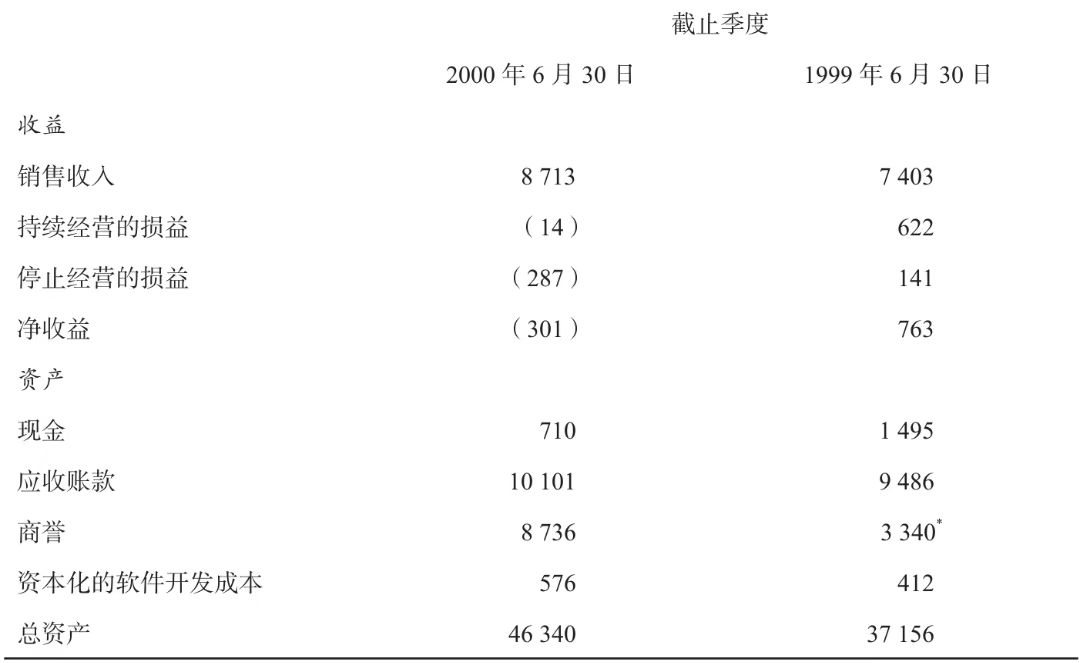
\includegraphics[width=\linewidth ,totalheight=0.95\textheight , keepaspectratio]{朗讯技术公司的财务信息.jpg}
\caption{朗讯技术公司的财务信息}
\end{figure}

所有的单位都是百万美元。

* 包括商誉在内的其他资产。

资料来源:朗讯公司的季度财务报告(表10-Q)。

对这位巨头的估价合理吗?让我们来看一看截止于2000年6月30日的季度财务报告所反映的一些基本信息。

更加仔细地阅读朗讯公司的财务报告,会感觉到警铃之声不绝于耳:

\begin{itemize}
\item 朗讯以48亿美元刚刚收购了一家光纤设备供应商Chromatis网络公司——这48亿美元中,有42亿美元属于“商誉”(高于账面值的成本)。Chromatis有150名员工,没有客户,没有任何销售收入,因此“商誉”这一项记录是不恰当的;或许,更为准确的称呼应该是“所怀有的希望”。如果Chromatis尚未成熟的产品还没成功,朗讯就必须减记这笔商誉,并且将其从未来的利润中扣除。

\item 有一条注释透露,朗讯已经向购买自己产品的人提供了15亿美元的信贷,朗讯还向在别处借款的客户提供3.5亿美元的担保。这些“客户融资”的总额,在一年之内增加了一倍——这表明,购货方已经快要拿不出资金来购买朗讯的产品了。如果这些客户没有钱偿还朗讯的债务,情况会如何?

\item 最后,朗讯将开发新软件的成本作为“资本资产”。这本来就不是一笔资产,难道这不是应该从利润中扣除的一项日常业务费用吗?
\end{itemize}

结论:2001年8月,朗讯关闭了Chromatis 这一部门,原因据说是其产品只有两个客户感兴趣。2001年财务年度,朗讯亏损了162亿美元;2002年财务年度,又亏损了119亿美元。这些亏损额中包括:35亿美元的“不良债务和客户融资备抵”,41亿美元的“与商誉相关的减损”,以及3.62亿美元“与资本化软件相关的”费用扣除。

朗讯的股价从2000年6月30日的51.062美元,降到了2002年年底的1.26美元——两年半之内,其市值几乎亏损了1 900亿美元。

\subsection{并购魔术师}
说到泰克国际有限公司(Tyco International Ltd.),我们只能转述丘吉尔说过的一句话:有史以来,从没有过如此少的几个人,能够欺骗如此多的公众。从1997年到2001年,这家位于百慕大的综合大企业总共花了370多亿美元(其中大多数为泰克股份)去并购其他公司,就像伊梅尔达·马科斯(Imelda Marcos)买鞋子那样频繁。根据其年度报告,2000年财务年度,泰克并购了“大约200家公司”——平均算下来每两天要收购不止一家公司。

结果如何呢?泰克的规模急剧增大;在5年内,销售收入从76亿美元,增加到了340亿美元,营业利润也从4.76亿美元的亏损转变成了62亿美元的盈利。难怪2001年年底,该公司的总市值高达1 140亿美元。

\begin{figure}[H]
\centering
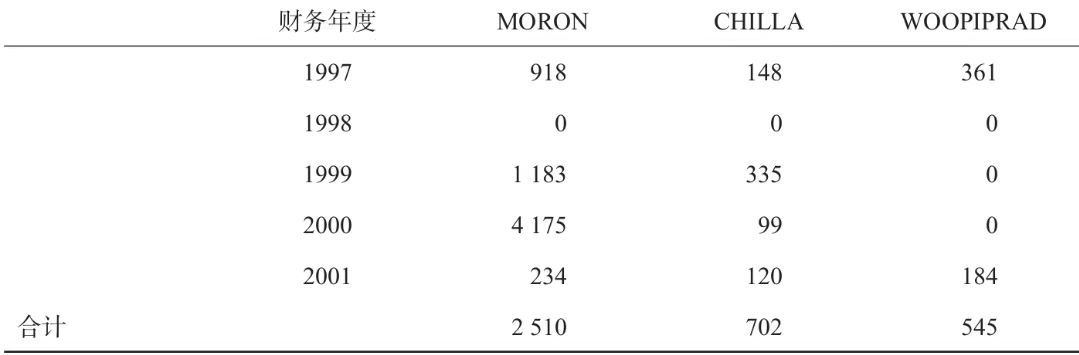
\includegraphics[width=\linewidth ,totalheight=0.95\textheight , keepaspectratio]{泰克国际有限公司的财务信息.jpg}
\caption{泰克国际有限公司的财务信息}
\end{figure}

所有数据都来自于原始报告,单位是千万美元。

“并购”总额中,不包括权益联合的交易。

资料来源:泰克国际的年度报告(表10-K)。

然而,泰克的财务报告至少也与其增长速度一样,令人难以想象。几乎在每一年,都报告有数亿美元与并购相关的费用产生。这些费用主要包括三类:

\begin{enumerate}
\item “并购”、“重组”或“其他一次性的”成本。
\item “长期资产损耗的费用”。
\item “购买在途研发产生的冲销额”。
\end{enumerate}

为了简便,我们将第一种费用简称为MORON,第二种简称为CHILLA,第三种简称为WOOPIPRAD。它们是在什么时间出现的呢?

正如你所看到的,MORON费用(应该是一次性的)在5年中出现了4次,其总额高达25亿美元。CHILLA也经常出现,并且总额超出了7亿美元。WOOPIPRAD大约有5亿美元。

聪明的投资者可能会问:
\begin{itemize}
\item 如果泰克借助并购求增长的策略是一个如此巧妙的想法,那么它为什么平均每年要花7.5亿美元才能将这项业务完成?
\item 如果(正如人们明显看到的)泰克不从事生产活动,而只是收购从事生产活动的其他公司,那么MORON这一项费用为什么会是“一次性的”?它们难道不正是泰克正常业务成本的一部分吗?
\item 随着以往并购的会计费用使每一年的利润都被看好,谁知道下一年的情况将会是怎样的?
\end{itemize}

实际上,投资者甚至不知道泰克过去的利润是多少。1999年,在美国证券交易委员会对其进行会计审核后,泰克反过来又在1998年的费用中增加了2.57亿美元的MORON费用——这意味着那些“一次性的”成本实际上又在1998年出现了。与此同时,泰克公司更改了1999年最初所报告的费用:MORON这一项降为9.29亿美元,而CHILLA这一项上升到5.07亿美元。

显然,泰克的规模正在扩大,但是,其利润率也在增长吗?外人无法准确地知道。

结论:在2002年财务年度,泰克亏损了94亿美元。其股价在2001年年底收于58.9美元,而2002年年底只有17.08美元——一年之内亏损了71\%。

\subsection{蛇吞象}
2000年1月10日,美国在线公司和时代华纳公司宣布,它们将进行一项初始价值高达1 560亿美元的合并。

截止于1999年12月31日,美国在线拥有103亿美元的资产,公司前12个月的营业收入为57亿美元。另一方面,时代华纳拥有521亿美元的资产,以及273亿美元的营业收入。除了股票估值这一项之外,从其他各方面看,时代华纳的规模都要大许多。由于美国在线仅凭自己所在的互联网行业就使得投资者痴迷于它,因此,其股价令人瞠目地达到了其利润的164倍。时代华纳从事有线电视、电影、音乐和杂志等多项业务,其股价大约只有利润的50倍。

在宣布这项交易时,两家公司都称这是一次“平等的战略合并”。时代华纳的董事会主席杰拉尔德·莱文声称:“对于与美国在线时代华纳有关系的任何人来说,都将面临着无数的机会。”——尤其是对于其股东而言,他补充说。

想到其股票最终将贴上互联网宠儿的标志而欣喜若狂,因此,时代华纳的股东以压倒性的优势批准了这笔交易。然而,他们却忽视了这样几点:

\begin{itemize}
\item 根据这次“平等的合并”,美国在线股东将拥有公司合并后55\%的股份——尽管时代华纳的规模是美国在线的5倍。
\item 3年内,美国证券交易委员会曾两次调查美国在线营销成本的会计记录是否恰当。
\item 美国在线总资产中,有将近一半(49亿美元)是由“待售股份”组成的。如果公开上市的技术股下跌,这将会使该公司的基础资产大多化为泡影。
\end{itemize}

结论:2001年1月11日,两家企业最终完成了合并。2001年,新组建的美国在线时代华纳亏损了49亿美元,而且在2002年又亏损了987亿美元(这是有史以来所有公司亏损中最大的一笔金额)。大多数亏损来自于美国在线价值的减记。到了2002年年底,莱文当初预计会面临着“无数”机会的股东没有任何收获,相反,自从交易首次宣布以来,他们的股票价值大约亏损了80\%。

\subsection{投资幼儿园会失败吗}
1999年5月20日,eToys公司向公众发售了8\%的股份。华尔街最有名气的4家投资银行——高盛、BancBoston Robertson Stephens、Donaldson,Lufkin \& Jenrette和美林——以每股20美元的价格承销了832万股,为公司筹集了1.664亿美元资金。该股票价格急速上涨后,收于76.5625美元,在首个交易日就获利282.8\%。按照这一价格,eToys(它拥有1.02亿股)的市值高达78亿美元。

股票购买者得到了什么?前一年,eToys公司的销售额上升了42.61倍,仅最后一个季度,它又增加了7.5万个客户。然而,经营20个月之后,eToys的总销售额为3 060万美元,并且有3 080万美元的净亏损——这意味着,eToys每卖出1美元的玩具,就要花费2美元。

IPO招股说明书还透露,eToys将使用出售股票的部分收入来收购另一家网络公司BabyCenter——前一年,BabyCenter的销售额为480万美元,亏损为450万美元。(要收购这家公司,eToys只需支付2.05亿美元。)eToys还要“预留”4 060万份普通股,以便将来出售给其管理层。因此,如果eToys能够赚钱的话,其净收益将在1.43亿份股票之间进行分配,而不是在1.02亿份股票之间进行分配——这将使得未来的每股收益下降近三分之一。

把eToys与其最大的竞争对手玩具反斗城(Toys“R”Us)进行对比后,会使人感到非常惊讶。前3个月内,玩具反斗城公司获得了2 700万美元的净收益,而且其销售额是eToys全年的70多倍。然而,从图17-3中可以看到,eToys的股市估价比玩具反斗城高出近20亿美元。

结论:2001年3月7日,在公开上市后不久,净亏损超过3.98亿美元之后,eToys公司提出了破产保护申请。该公司的股票在1999年10月曾达到每股86美元的最高价,但最后几乎一文不值了。


\section{股东与管理层:股息政策}
从1934年开始,我们就在自己的作品中主张,股东应该对公司管理层抱有更加明智和积极的态度。我们要求股东慷慨地对待那些工作出色的管理层。同时,我们还要求他们在结果比想象的要差时,力求得到清楚和令人满意的解答;并且,要积极改进或撤换业绩明显较差的管理层。下列情况下股东有理由对管理层的能力产生怀疑;(1)其结果本身不能令人满意;(2)其结果比类似环境下其他公司的要差;(3)其结果导致股票价格长期不能令人满意。

在过去的36年中,众多股东并没有通过理智的行为获得任何实际结果。一位明智的斗士(如果真有这样一个人的话)将从这一迹象中看到,他一直是在浪费自己的时间,因此最好是放弃这场战斗。情况表明,我们的事业尚未丧失;它被一项新的发展——人们所称的并购或竞价并购——拯救了。在第8章我们曾说过,较差的管理层会导致较差的股价。反过来,较低的股价会吸引那些对自己的业务多元化感兴趣的公司的注意力——现在这类公司有很多。众多此类并购交易都是通过下列方式完成的:与现有的管理层达成协议;收购市场上的股份;由并购公司总部提出并购要约。并购的报价,一般都大致相当于有较好能力的管理层能给企业带来的价值。因此,在许多情况下,对公司事务不太积极的股东大众,会因为“外部人”的行为而得到拯救。这些外部人有可能是自愿从事此类业务的有事业心的个人或群体。

可以说,在绝大多数情况下,较差的管理层不会因为“股东大众”的行为而改变,只会因为某一个人或少数几个人获得控制权而改变。那时候,这种情况的频繁发生,引起了一般上市公司的管理层(包括董事会在内)的注意:如果自己的经营结果及相应的股票价格非常难以令人满意,那么就可能成为被他人成功并购的一个目标。因此,董事会可能会在履行其基本职责上比以前更为积极,以确保自己的公司有一个令人满意的最高管理层。与以前相比,近几年公司总裁的更换更加频繁了。

并非所有难以令人满意的公司都从这种发展变化中获得了好处。同样,这种改变经常发生在经历了长时期的不利结果而无力纠正的情况下,而且还有赖于大量失望的股东低价抛售股票,使积极的外部投资者获得控股地位。股东大众的确可以通过支持改进管理层和管理政策的行动来帮助自己,但是由于这一想法太不现实,因此不必在本书中进一步讨论了。那些有足够的勇气出席股东年会(一般情况下,这是完全没有用的)的个人股东,不需要我们去告诉他们应该向管理层提出哪些问题。对其他股东而言,这种建议是白费口舌。尽管如此,在这一节的最后,我们还是请求股东客观细致地对待其他股东(他们想要纠正公司明显不能令人满意的管理状态)送给自己的代理材料。

\subsection{股东和股息政策}
过去,股息政策是股东大众(或“少数派”)与管理层经常争论的问题。一般情况下,股东希望分得更多的股息,而管理层则倾向于将利润留在企业,“以增强企业的实力”。他们要求股东牺牲眼前利益来换取企业利益以及自己的长远利益。但是,近几年,投资者对股息的态度正在逐渐发生重大变化。目前,赞成支付少量股息的基本理由,已不再是公司“需要”资金,而是因为公司利用这些资金扩展盈利业务之后,可以给股东带来直接和间接的好处。多年以前,实力较弱的公司一般都不得不保留自己的利润,而不会按通常的做法支付60\%~75\%的股息。这种做法几乎总是会使其股票的市场价格处于不利地位。如今,很有可能发生的情况是,实力强劲和快速增长的企业,在投资者和投机者的许可下,保留本应支付的股息。

总有貌似有力的理论认为,企业留存利润的再投资可以带来更大的利润增长。但是,也有一些强烈反对的意见,比如:有人认为,利润是“属于”股东的,因此他们有权要求管理层在谨慎的范围内支付这些利润;许多股东需要依靠股息来维持生活;股东从利润中得到的股息,才是“实实在在的钱”,而留在公司的利润不一定会成为股东日后的有形资产。事实上,这些相反的观点有很强的说服力,因此,长期以来,股市一直偏爱股息支付比较大方的公司,而不太看好不支付股息或股息支付较少的公司。

过去20年内,“利润再投资”理论越来越受到重视。以往的增长记录越好,投资者和投机者就越乐意接受支付较低股息的政策。这种观点的影响十分强大,因此,许多情况下,增长最好的公司的股息支付率即使为零,似乎也不会对其股票价格产生任何实际的影响。

德州仪器公司的历史,就是这方面最突出的一个例子。该公司普通股的股价,从1953年的5美元,上涨到1960年的256美元;同时,每股收益从43美分涨到3.91美元。然而,公司却没有支付任何股息。(从1962年开始支付现金股息,但是当年的每股收益降到2.14美元,同时股价也大幅降到了49美元这一最低水平。)

另一个极端的例子是Superior石油公司。1948年,该公司报告的每股收益为35.26美元,每股支付3美元的股息,且股价高达235美元。1953年,股息降到了每股1美元,最高股价却达到了660美元。1957年,完全没有支付股息,股价却高达2 000美元。这一非同寻常的股票,后来在1962年降到每股795美元,这时公司的每股收益为49.5美元,支付的每股股息为7.5美元。

投资者对成长型公司股息政策的看法还很不明确。矛盾的观点可以通过两家大公司——美国电话电报公司和IBM——的例子很好地反映出来。美国电话电报公司的股票被看做是有很好的增长潜力的,这可以从下列事实中看到:1961年,其股价是当年利润的25倍。然而,该公司的现金股息政策被投资者和投机者看成是首先要考虑的因素,甚至一些即将增加股息支付率的谣言,都会使其行市做出积极的反应。另一方面,人们似乎很少关注IBM的现金股息——在价格较高的1960年,只有0.5\%的股息收益;在1970年年底,有1.5\%的股息收益。(但是,两家公司的股票分割都会对股市产生强有力的影响。)

市场对现金股息政策的判断,似乎正朝着下列方向发展:重点强调增长率的股票,被看做是“收入型股票”,长期决定此类股票价格的主要是股息支付率。在另一个相反的方面,被明确看做是快速增长型的股票,其价值主要取决于(比如今后10年内的)预期增长率,同时,现金股息支付率大多不在人们的考虑之内。

尽管上述观点能够反映目前的发展趋势,但它决不是针对所有普通股状况给出的一个明确指导,而且,这或许还不能代表大多数的普通股。首先,许多公司的地位都处在成长型企业和非成长型企业之间。这种情况下,很难说增长率这一因素有多么重要,因此,市场的观点在不同年份之间会发生极大的改变。其次,要求增长较慢的公司支付较多的现金股息,这似乎有些矛盾。因为,这些一般都是事业不太兴旺的企业,而且,按照以往的观点,公司越兴旺,预计将来所支付的股息的数量和增长率都会更大一些。


我们认为,股东要么要求管理层按通常的做法支付利润(比如,大约支付三分之二),要么要求他们能够明确地证明,利润再投资使得每股收益获得了满意的增长。这种证明通常可以从公司明显的增长率中看到。但是,在其他许多情况下,较低的股息支付率显然是平均市价低于公允价值的原因,因此在这种情况下,股东完全有理由去进行调查,并且可以说出自己的不满。

许多情况下,公司在支付股息方面采取吝啬政策,是因为其财务实力相对较弱,需要以全部或大部分利润(加上折旧费)来偿付债务和增加自己的营运资本。这种情况下,股东就没有多少话可说了,或许只能批评管理层把公司的财务状况搞得如此难以令人满意。可是,一些业务不太兴旺的公司留存股息的明确目的在于扩张公司。我们感觉这种政策本身是不符合逻辑的,因此,在得到股东认可之前,必须要求公司做出完整的解释并给出令人信服的理由。从以往的记录来看,当一个企业业绩平平,而且管理层没有发生改变时,人们没有理由相信,所有者可以从自己的资金所带来的扩张中获得好处。

\subsection{股票形式的红利(红股)和股票分割}
重要的一点在于,投资者要理解(恰当意义上的)股票形式的红利与股票分割之间是有重大差别的。后者代表了普通股结构的改变,通常情况下,会以2比1或3比1来发行新股。发行的新股与过去一定时期的利润再投资没有关系。股票分割的目的是使每股的市场价格下降,其原因可能在于,这种较低的价格区间使得新旧股东更容易接受。股票分割可以借助于所谓的股票形式的红利来完成——这需要将一笔盈余账户转入到资本账户中去,也可以借助于面值的变化来完成——这不会影响到盈余账户。

我们所说的恰当的股票形式的红利,是指支付给股东的股息有实实在在的证据,或者是代表了特定的利润——这些利润在近期的较短时间内(比如在近两年之内)以股东账户对企业进行再投资。现在,人们都对这种做法表示认同:以宣布分配股票形式的红利时的价值大致代表这种形式的红利的价值,并将这笔价值按等值额从盈余账户转移到资本账户。因此,股票形式的红利金额一般都比较小,大多数情况下,都不会超过5\%。本质上讲,这类股票形式的红利的总体影响,类似于从利润中支付等额现金的同时,向股东额外出售总价值相等的股份。可是,与现金股息和认股权相结合的做法相比,直接分配股票形式的红利具有重要的税收优势——直接分配股票形式的红利几乎是公用事业公司标准的做法。

纽约股票交易所将股票分割和股票形式的红利之间的实际界线确定为25\%。达到或超过25\%的股票形式的红利分配,无需采用将其市值从盈余账户转到资本账户等做法。有些公司,尤其是一些银行,还在采用随意公布股票形式的红利的旧做法(比如,每股10\%,与近期利润无关系),这些情况会给财务领域带来一定的混乱。

长期以来,我们一直强烈主张在现金股息和股票形式的红利支付方面要有一个系统的、明确的政策。根据这种政策,定期支付的股票形式的红利将使企业再投资的利润全部或部分资本化。这种政策(涵盖100\%的再投资利润)已经被Purex公司、政府雇员保险公司以及其他几家公司所采纳。

研究形式的红利的大多数学者似乎对各种股票形式的红利都持否定态度。他们坚持认为,股票形式的红利不过是几份证券而已,它们没有给股东带来额外的好处,而且它们涉及一些不必要的费用和麻烦。我们认为,这完全是一个脱离实际的观点,它没有考虑到投资的实用性和心理现实。是的,定期支付的股票形式的红利(比如5\%),只改变了所有者的投资“形式”。他拥有了105股,而不是100股;但是,如果没有股票形式的红利,最初100股所代表的所有者权益与现在的105股是一样的。尽管如此,这种形式的改变对所有者来说是具有实际意义和实际价值的。如果他想兑现自己利润再投资的股份,那么他就可以将所获得的新的证券出售,而不必去拆散自己原有的证券。与以前100股的情况一样,他可以指望从105股中获得现金股息;如果没有股票形式的红利分配,现金股息增加5\%的可能性就要小一些。

与下列情况对比,就可以非常清楚地看到定期支付股票形式的红利这一政策的好处:公用事业企业经常采用的做法是,先支付大量的现金股息,然后以向股东出售额外股票(通过认购权)的形式,再将这部分现金中的大部分收回。正如我们前面所指出的,股东获取股票形式的红利的做法,与获取现金股息再加上认购权的通行做法相比没有什么区别,只不过他们可以省去现金股息的所得税。那些需要或希望获取最大的年现金流的人,可以在不增加股份的情况下将其股票形式的红利出售,这与目前出售认购权的做法是一样的。

以股票形式的红利替代现在的股息加认购权的做法,可以节省大量的所得税。我们强烈要求公用事业企业改变做法(尽管这会对美国的财政收入带来不利影响),因为我们确信,对一笔利润(股东实际上并没有得到这笔利润,因为公司通过出售股票又将这笔钱收回去了)再次征收(个人)所得税的做法是完全不公平的。

富有效率的公司一直在改进自己的设施、产品、会计方法、管理层培训计划以及劳资关系。现在,它们应该考虑如何改进自己的重大财务行为,其中包括股息政策。





\section{第19章点评}
\subsection{格雷厄姆为何会放弃努力}
在《聪明的投资者》这本书中,格雷厄姆对这一章内容的改动或许是最大的。在本书的第一版中,本章的内容只是两项内容中的一项——两项内容一共接近34页。最初的内容(“作为企业所有者的投资者”)涉及股东的投票权、评价公司管理层水平的方法,以及观察公司内部人员与外部投资者之间利益冲突的方法等。可是,在最后修订的这一版中,格雷厄姆将整个内容压缩成了只有关于股息的几页内容。

格雷厄姆为什么将原来的论述砍去了四分之三以上?经过了几十年的劝告之后,格雷厄姆显然放弃了希望:在监控公司管理者的行为方面,投资者永远都不会感兴趣。

可是,近期广泛出现的丑闻(比如,美国在线、安然、Global Crossing、Sprint、泰克和世界通信等大公司,在管理者行为不当、会计不透明和税收操纵等方面受到的指控)明确地告诉我们,格雷厄姆先前关于内部监督的告诫,比以往任何时候都显得更重要。下面我们将以如今发生的事件为例重新探讨这一话题。

\subsection{理论与实际的对比}
在本书的第一版(1949年)中,探讨“作为企业所有者的投资者”这一项内容时,格雷厄姆认为,从理论上讲,“股东这一群体拥有最大的权利。作为绝大多数,他们可以雇用和解聘公司管理层,因此,他们能让公司管理层完全服从于自己的意愿。”但是,从实践来看,格雷厄姆说:

\begin{quote}
“股东完全是无能的。作为一个群体,他们既没有表现出智慧,也没有表现出警觉。他们对管理层所建议的东西都去投票赞成,而不管管理层的的记录有多么糟糕。……想使一般的美国股东独立地采用理智的行动,惟一的办法就是对其当头一棒。……我们不得不指出这样一个似乎矛盾的事实:耶稣似乎是比美国股东更为现实的商人。”
\end{quote}

格雷厄姆想要你认识到一个基本但却十分深刻的事实:当你购买了某公司的股票时,你就成为该公司的所有者。包括CEO在内,公司的所有管理者都是在为你工作。公司的董事会必须对你的问题做出回答;公司的现金属于你;公司的业务是你的财产。如果你不喜欢公司的管理方式,你有权要求解雇管理者,更换董事,或者是将公司财产出售。“股东们”,格雷厄姆说,“应该明白过来了。”

\subsection{聪明的所有者}
如今,投资者已经忘记了格雷厄姆的忠告。他们在购买股票上花费大量的精力,在出售股票上花费很少的精力,然而,在拥有股票上却没有花任何精力。“毫无疑问”,格雷厄姆提醒我们,“无论是即将成为股东,还是已经成为股东,都需要有细致的判断。”

这样,作为一位聪明的投资者,你如何才能成为一位聪明的所有者呢?格雷厄姆首先告诉我们,“股东只需要关注两类基本问题。

\begin{enumerate}
\item 企业管理层是否具备应有的效率?
\item 普通的外部股东的权益是否得到了适当的认可?”
\end{enumerate}

将公司的盈利能力、规模和竞争力等方面与同类公司进行对比,就可以判断公司管理层的效率。如果你得出的结论是管理层缺乏效率,那么该怎么办呢?这时,格雷厄姆认为:

\begin{quote}
少数重要的股东应该确信公司需要改革,并且朝着这一方向努力。其次,普通的股东应该公正地阅读代理材料,并对双方的观点进行权衡。他们至少应该知道公司的业务何时开始出现问题,而且不能只听信现有的管理层以虚假的陈词滥调所做的辩护。第三,如果数据清楚地表明公司的经营结果大大低于平均水平,那么最好是有这样一种惯例:请公司外部的企业策划师(business engineer)来对管理层的政策和能力做出评判。
\end{quote}

什么是“代理材料”,格雷厄姆为什么坚持认为应该阅读这份材料?在发给每位股东的代理报告中,公司会宣布股东大会的日程,并详细披露其管理者和董事的薪酬和股份,以及公司内部人员和公司之间交易的相关信息。股东要投票表决挑选出审计师事务所以及公司的董事。如果你根据常识来阅读代理报告,那么这份材料就类似于煤矿中的金丝雀——一个早期预警信号(金丝雀对于瓦斯的敏感性远远高于人类,当瓦斯浓度过高时,金丝雀就会停止歌唱或死去,因此在煤矿中能够起到预警作用——译者注)。

然而,一般情况下,有三分之一到二分之一的个人投资者不会针对代理报告中的问题投票。他们会去阅读代理报告吗?

理解并对代理报告进行投票,是对信息进行跟踪的聪明投资者的基本行为,而且,根据自己的良心投票是一个好公民应有的行为。无论你拥有公司股份的10\%,还是只拥有微不足道的100股(只占公司股份的百万分之一),这并不重要。如果你从未阅读过自己股票的代理报告,而公司破产了,那么你只能怪自己。如果你阅读了代理报告,并发现了一些使人感到不安的东西,那么:

\begin{itemize}
\item 投每位董事的反对票,以让其知道你不同意他们的行为
\item 参加股东大会,并阐述自己的权利
\item 找一个针对股票业务的网上信息公告栏,号召其他投资者加入到你的行动中来
\end{itemize}

格雷厄姆的另外一个想法对如今的投资者会有帮助:

\begin{quote}
……挑选一位或多位职业董事和独立董事是有好处的。这些人必须有广泛的商界经历,能够从不同的专业角度来观察企业的问题。……他们要提供一份独立的年度报告,报告直接面向股东,并且要包含在重大问题上的一些观点——这些问题是企业所有者所关注的:企业给外部股东带来的结果,符合正常管理条件下的预期结果吗?如果不符合,那么原因是什么——以及应该怎么办?
\end{quote}

人们可以想象,格雷厄姆的建议将在公司密友和高尔夫伙伴之间造成多大的恐慌(如今的“独立”董事大多是由他们来担任的)。(我们并不认为这会使得他们的脊背发凉,因为大多数独立董事似乎没有脊梁。)

\subsection{到底是谁的钱}
现在让我们来看格雷厄姆的第二个标准:管理层的行为是否最有利于外部投资者。管理者总是告诉股东,他们最了解公司的资金应该怎么使用。格雷厄姆正好看穿了管理者这种糊弄人的话:

\begin{quote}
公司的管理层有可能把业务经营得很好,但却不能给外部股东带来理想的结果,因为公司的效率取决于业务活动,不一定反映了资本的最有效利用。有效经营的目标是以最低的成本进行生产,并且出售最赚钱的东西。有效融资要求股东资金的使用最符合他们的利益。这是目前的管理层不感兴趣的问题。实际上,公司管理层总是想尽可能从所有者那里获得资本,以尽量减少自己的财务问题。所以,一般的管理层都会利用过多的资本来开展经营——只要股东许可的话(情况通常是这样的)。
\end{quote}


20世纪90年代末和21世纪初,一些主要的技术型公司的管理层,将“家长最懂行”这种态度发展到了新的极致。其理由是这样的:既然我们能够替你进行投资,并将投资转变为股价的上涨,你为什么要求支付股息呢?仅看一看我们的股价上涨得有多快——难道这还不能证明我们比你更能使资金增值吗?

难以置信的是,投资者完全接受了这种观点。“家长最懂行”因此而成为一种信条:到了1999年,首次公开发行股票的公司中,只有3.7\%在当年支付了股息,而20世纪60年代所有IPO支付股息的平均比重为72.1\%。...

可是,“家长最懂行”只不过是一句假话。尽管有些公司使自己的资金发挥了很好的作用,但更多的公司则面对着其他状况:有的只是把资金浪费了,而有的资金因增长过快超出了应有的需求。

关于第一类公司,请看这样几个例子。冒然地进入了食品杂货业和汽油行业之后,价格线网络公司(Priceline.com)在2000年亏损了6 700万美元;由于对Webvan和Ashford等网络公司的“投资”遭遇巨大失败,亚马逊网络公司给股东的财富至少造成了2.33亿美元的损失。迄今为止,最大的两笔亏损记录(2001年JDS Uniphase公司的560亿美元的亏损,以及2002年美国在线时代华纳公司990亿美元的亏损),是在这些公司不愿支付股息而决定与股价高估得令人恐怖的企业合并时发生的。

就第二类公司而言,我们来看这样几个例子。2001年年底,甲骨文公司积累了50亿美元的现金。思科公司至少储存了75亿美元的现金。微软积累的现金高达382亿美元——而且还在以平均每小时200万美元的速度增加。不知道比尔·盖茨预计将来会有多少困难?

这些事例清楚地表明,许多公司都不知道如何将闲置现金用来赚取额外的回报。统计方面的证据能够告诉我们什么呢?

\begin{itemize}
\item 罗伯特·阿诺特和克利福德·阿斯尼斯等货币经理的研究表明,当期股息较低的时候,公司未来的利润最终也会较低。当期股息较高的时候,未来的利润也较高。在10年期内,股息较高的公司的平均利润增长率,比股息较低的公司要高出3.9个点。
\item 哥伦比亚大学的会计学教授多伦·尼斯姆和阿米尔·齐夫的研究发现,增加股息的公司不仅有更高的股票回报率,而且“其股息的增加还会使得此后至少未来4年内的利润率(更高)”。
\end{itemize}

总之,当管理者说自己能够比你更好地使现金发挥作用时,他们的话语大多数是错的。支付股息不一定保证是最好的结果,但是这的确可以使得一般的股票回报得以改进,因为这至少从管理者手中挤压出了一部分可能会被浪费或储存起来的现金。


\subsection{贵买贱卖}
公司以闲置现金买回自己的股票是较好的办法,这一观点如何?当公司购回其中的一些股票时,现有的股票数量会下降。即使公司的净收入不变,其每股收益也会上升,原因在于,其总利润将分摊到更少的股份数之中。反过来,这会使得股价上升。更有利的是,与股息不同,回购股份对持股的投资者来说是免税的。因此,它在使股票升值的同时,不会加重税收负担。所以,如果股价便宜,将闲置资金用于回购股票,是利用公司资本的一个很好的方法。

从理论上讲,所有这些都是正确的。遗憾的是,在现实世界中,股票回购只会带来一种不祥的后果。由于发放的股票期权已占高管薪酬的很大一部分比重,因此,许多公司(尤其是高科技行业的公司)必须向行使股票期权的管理者发售上百万份股票。但是,这会抬升现有股份的数量,并降低每股收益。为了抵消这种稀释作用,公司必须回过头来在公开市场回购上百万份股票。2000年,公司全部的净收入中,竟然有高达41.8\%的净收入用于回购自己的股份;而1980年,这一比重只有4.8\%。

让我们来看软件行业的巨头甲骨文公司的情况。从1999年1月1日到2000年5月31日,甲骨文向其高管发行了1.01亿股普通股,并且向员工发行了2 600万股普通股——筹集到了4.84亿美元的资金。与此同时,为了防止行使股票期权给每股收益带来的稀释作用,甲骨文花费53亿美元(占当年总收入的52\%)回购了2.907亿股。甲骨文向公司内部人员出售股票的平均价为每股3.53美元,而回购股票的平均价为每股18.26美元。贵买贱卖:这是“提升”股东价值的方法吗?

2002年,甲骨文的股价还不到其2000年最高值的一半。既然股价更便宜了,甲骨文会抓紧时间回购更多的股票吗?从2001年6月1日到2002年5月31日,甲骨文将回购的股票压缩到28亿美元。这显然是因为其高管和员工这一年行使的股票期权较少。在其他十几家技术型公司中,也明显存在着这种贵买贱卖的现象。

这是为什么?是因为有两个令人意外的因素在发挥作用:

\begin{itemize}
\item 高管和员工行使股票期权会给公司带来税收上的优惠(国税局将行使的股票期权看做公司的“薪酬费用”)。比如,在2000~2002年财务年度,甲骨文因为公司内部人员兑现期权而获得了16.9亿美元的税收优惠。1999年和2000年,由于其高管和员工获取了19亿美元的股票期权利润,Sprint公司自己也获得了6.78亿美元的税收优惠。
\item 薪酬中股票期权占很大比重的高管,从自身利益出发,必然会赞成股票回购,而不赞成股息派发。为什么?从技术上讲,期权的价值会随着股价波动幅度的增加而增加。但是,股息会抑制股价的波动性。所以,如果管理者增加股息,就会降低自己拥有的股票期权的价值。
\end{itemize}

难怪CEO们更愿意回购股票而不愿意支付股息了。不管股价如何波动和高估,也不管这会浪费外部股东多少资金。

\subsection{让股票期权公开}
最终,懒散的投资者只能让公司肆无忌惮地给高管发放高额的薪酬。1997年,苹果电脑公司的共同创始人史蒂夫·乔布斯以“临时”首席执行官的身份重返公司。由于已经很富有,乔布斯坚持每年只要1美元的现金薪酬。1999年年底,为了感谢这位“在过去的两年半内没有获取薪酬”的CEO,公司董事会送给了乔布斯一架Gulfstream喷气飞机——这就花费了公司9 000万美元。接下来的一个月,乔布斯同意从头衔中取消“临时”两个字,这样董事会分给了他2 000万美元的股票期权。(此时,乔布斯总共持有2 000股苹果股份。)

分配这种股票期权的原则是使管理者的利益与外部投资者的利益一致。如果你是苹果股份的外部持有者,那么只有当苹果的股票获得很好的回报时,你才允许公司的管理者得到奖励。对于你和公司其他的所有者而言,任何其他做法都是不公平的。然而,正如先锋基金的前董事会主席约翰·博格尔所说的,几乎所有的管理者都会在行使期权后,立即将所获股票出售。一下子出售上百万份股票以获取眼前的利润,这种行为怎么可能与忠实于公司的长期股东的利益是一致的?

以乔布斯的情况为例,如果苹果公司的股价仅按5\%的年率增长到2010年年初,他就能够将股票期权兑现为5.483亿美元。换句话讲,即使苹果的股票回报率还不到整个股市长期平均回报率的一半,乔布斯也会有5亿美元的意外收获。乔布斯的利益与苹果公司股东的利益相一致吗?或者说,苹果公司的董事会是否滥用了公司股东对自己的信任?

仔细阅读代理报告之后,聪明的所有者将会投票否决下列高管薪酬计划:利用股票期权将公司3\%以上的现有股份变成管理者所有。凡是不与公平和持久的公司优异结果(比如,至少5年内的股票回报要高于同行业的平均水平)挂钩的股票期权计划都应该被否决。如果他给你带来的结果不理想,那么这位CEO就不应该使自己变得富有。

\subsection{最后一点思考}
让我们回头来看格雷厄姆的建议:公司的每一位独立董事都应该以书面形式向股东提供报告,说明企业是否从实际所有者的利益出发在开展经营。如果独立董事还应该评判公司股息政策和股票回购政策的合理性,情况会如何?如果他们应该准确地说明自己是如何判断公司高管薪酬的合理性的,情况会如何?如果每一位投资者都成为聪明的所有者,并且去实际阅读公司的财务报告,情况又会如何?



\section{作为投资中心思想的“安全边际”}
在古老的传说中,一些智者最终将人世间的历史归纳成一句话:“这,也将成为过去。”当我们需要总结出稳健投资的秘密时,可以用安全边际(margin of safety)这一座右铭来代表。这是一条主线,它贯穿于前面所有关于投资策略的论述之中,有时被明确表达出来,而有时则表达得不太直接。现在,让我们以连贯的论述来简要追踪这一思想。

所有有经验的投资者都能意识到,在挑选恰当的债券和优先股时,“安全边际”这一概念至关重要。比如,要想达到债券投资级别的话,那么铁路公司的(税前)利润至少应该在该公司总固定费用的5倍以上,并且连续几年保持这样的业绩。这种过去能够使利润超出利息要求的能力构成了一种安全边际——一旦公司未来的净收益下降,它可以防止投资者遭受损失或失败。(超出费用的幅度也可以用其他方式来表达,比如把扣除利息之后的余额计算在内,公司的收益或利润还可以下降多大的百分比,然而,其根本思想是一样的。)

债券投资者并没有期望未来的平均利润结果与过去的情况一样。如果他能确保这一点,所需要的安全边际就可以比较小。他也不可能有把握地知道,未来的利润与过去的相比,是会极大地改善,还是会极大地恶化。如果能做到这一点,他就会通过仔细预测出的收益账户来反映其安全边际,而不会去强调过去的记录所反映的安全边际。本质上,这里的安全边际的作用是使投资者不必对未来做出准确的预测。如果安全边际较大,那么就足以保证未来的利润不会大大低于过去的情况,从而使得投资者不会因为时间的变化而遭遇风险。

从另一方面看,债券的安全边际可以通过比较企业的总价值与债务的规模而计算出来。(优先股也可以采用这种计算方法。)如果企业拥有1 000万美元的债务,而其公允价值为3 000万美元,那么在债券持有人遭受亏损之前,企业的价值还有三分之二的下降空间(至少从理论上讲是如此)。这部分高于债务的额外价值,或“缓冲价值”,可以利用一定年份内次级股份的平均市场价大致计算出来。由于平均股价一般与平均盈利能力相关联,因此,“企业价值”超出债务的差额和利润超出费用的差额,在大多数情况下都会带来同样的结果。

关于安全边际这一概念在“固定价值投资”方面的应用,我们就讲到这里了。这一概念可以用于普通股领域吗?是的,但要做一些必要的修改。

如果普通股能够像优质债券那样达到足够的安全边际,那么它们也可以被看做是稳妥的。比如,下列情况下就是如此:公司只拥有普通股,而在危机情况下,这些普通股的售价要低于公司可能以财产和盈利能力为稳固基础而发行的债券的价值。1932~1933年股价低迷时期,一些财务实力很强的工业企业就处于这种地位。在此类情况下,投资者既能获得与债券一样的安全边际,又能够获得普通股固有的本金升值和更大的盈利机会。(惟一缺少的是,不能依法要求获得股息“或其他的偿付”。但是,与所获得的好处相比,这只是一个小小的缺憾。)在这种情况下购买的普通股,一般能较好地兼顾到安全边际和盈利性这两个方面,尽管这种情况并不常见。作为这方面较新的一个例子,让我们再来看National Presto工业公司的股票。1972年,该公司股票的总市值为4 300万美元。由于公司近期的税前利润为1 600万美元,因此能够轻易地支持这部分股票的价值。

就一般的(通常情况下用于投资的)普通股而言,其安全边际表现在预期的盈利能力大大高于债券现有的利率。在本书的前几版中,我们以下列数据为例阐述过这一点。

假设一般情况下股票的盈利能力为9\%,债券的利率为4\%。那么,股票购买者平均每年有5\%的利润是属于自己的。多出的这部分利润中,有一些向他支付了股息——即使他将这部分花掉,这也成为他的总投资结果的一部分。未分配的余额以他的账户用于企业的再投资。在许多情况下,这种再投资所获取的利润,比不上盈利能力以及股票价值的增加。(这就是为什么市场总是更看重将利润用于股息分配,而不太看重企业的利润留存。)可是,总的看来,利润再投资给公司带来的盈余增长与公司价值的增长之间必然有着密切的联系。

在10年之内,高于债券利率的累积股票盈利能力,一般会达到股票购买价的50\%。这一数字足以提供一种非常可靠的安全边际,在有利条件下,这一安全边际可以防止或降低亏损。如果在20种或更多种股票构成的分散化组合中,每一种股票都能达到这一安全边际,那么,在“比较正常的情况下”,获得有利结果的概率将会很大。这就是投资于有代表性的普通股的策略并不要求有很强的分析和预见能力就可以取得成功的原因。如果按几年的市场平均水平买股票,那么,所支付的价格应该能够确保获得足够的安全边际。投资者面对的危险在于,集中购买价位很高的股票,或者购买不具有代表性的普通股(它们的盈利能力下降的风险要大于一般水平)。

正如我们所看到的,1972年的普通股投资面临的整个问题在于这样一个事实:“在通常情况下”,现在的盈利能力要大大低于股价的9\%。让我们假设,通过在某种程度上集中购买大公司的低市盈率股份,一位防御型投资者现在可以获得股价为近期利润12倍的股票——利润率为股票购买价的8.33\%。他还可以得到大约4\%的股息,而且他还以自己的账户把占股价4.33\%的利润用于企业的再投资。按照这种做法,10年内股票盈利能力超出债券利息的这一部分仍然太小,而且还不到应有的安全边际。因此我们认为现在面临着实际的风险,即使是由稳妥的普通股构成的分散化组合,这种风险仍然有可能被股票组合将来的利润完全抵消;而且,事实上投资者可能不得不去承担这种风险,否则,他有可能要面对更大的风险——在美元持续贬值的情况下,却只持有固定的应付债权。然而,投资者最好能够认识到,以前的低风险和高收益组合已不复存在(并尽量把这作为一种理念)。

可是,付太高的价格购买优质股的风险(尽管是实际存在的),并不是普通的证券购买者面对的主要风险。多年的观察结果告诉我们,投资者的主要亏损来自于经济状况有利时期所购买的劣质证券。证券购买者把当期较高的利润当成了“盈利能力”,并且认为业务兴旺就等同于安全边际。正是在这样的年代,质量较差的债券和优先股才能大约按平价出售给公众。这是因为它们的收益率稍高一些,或者是因为它们所具有的转换权的误导。同时,也正是在这种情况下,不知名的公司的普通股才能凭借两三年快速增长的实力,按大大高于其有形投资的价格发行出去。

这些证券不可能在真正意义上提供合理的安全边际。利息费用和优先股股息的保障必须经过多年的检验——最好是包含了像1970~1971年那样经济较差的时期。就普通股的利润而言,一般也是这样的,如果它们要想较好地反映公司的盈利能力。因此,有利条件下的大多数投资,即使是按有利价格购买的,也必然会在不利条件下经历令人不安的价格下跌(而且,这种情况经常是在不利条件出现之前就已经发生了)。投资者也不能满怀信心地指望最终的反弹,尽管有时会发生这种情况,因为并没有真正意义上的安全边际来保证他度过这一困境。

成长股投资的理念在一定程度上类似于安全边际原则,又在一定程度上与该原则相抵触。成长股的购买者所依赖的预期盈利能力,要大于过去的平均盈利能力。因此,可以说,他在计算安全边际时,以预期利润取代了以往的利润记录。从投资理论上讲,人们没有理由认为,细心估算出的未来利润,比过去单纯的利润记录更缺乏指导作用。事实上,证券分析已经越来越看重有能力的分析师对未来情况所做出的评价。因此,与普通投资一样,成长股的分析方法得出的安全边际也是可靠的——只要对未来的计算是稳妥的,而且只要相对于其购买价而言存在着令人满意的安全边际。

成长股投资计划的风险也正是表现在这一点上。在广受欢迎的情况下,市场一般会使成长股的价格不能得到稳妥预测的未来利润的恰当保护。(谨慎投资的基本法则是,所有估算出来的结果,如果与过去的情况不同,都必须至少稍稍偏保守一些。)安全边际总是依赖于所支付的价格。如果某种价格下的安全性较大,较高价格下的安全边际就较小,价格更高时就没有了安全边际。如果按照我们所说的,大多数成长股的市场平均价格水平太高而无法向买方提供适当的安全边际,那么,在这一领域简单地使用分散化购买的方法是不会获得令人满意的结果的。聪明的个人投资者需要有相当高的预见性和判断力,才能通过选择来克服这种股票的一般市场价格总体上所具有的风险。

在证券被低估的领域或廉价证券领域,安全边际的思想表现得更清楚。在此,我们给出的定义是,证券的市场价格高于证券的评估价格的差额。这一差额反映了证券的安全边际。它可以吸纳计算失误或情况较差所造成的影响。廉价证券的购买者尤其重视其投资能够抵御不利影响的能力。因为,在大多数情况下,他都不会对公司的前景抱有实际的热情。是的,如果前景肯定不好,那么无论证券价格多么低,投资者最好还是不要去购买。可是,被低估的证券都来自于许多这样的企业(这种企业或许是大多数):该企业的未来既没有明显的吸引力,也不是明显没有希望。如果廉价购买到这些证券后,即使盈利能力有一定程度的下降,仍然希望可以获得满意的投资结果的话,此时,安全边际就能发挥应有的作用。

\subsection{分散化理论}
安全边际这一概念与分散化原则有着密切的逻辑联系,两者是相互关联的。投资者即使有一定的安全边际,个别证券还是有可能出现不好的结果。因为安全边际只能保证盈利的机会大于亏损的机会,并不能保证不会出现亏损。但是,当能购买的具有安全边际的证券种类越来越多时,总体利润超过总体亏损的可能性就越来越大。这就是保险业务的基本思想。

分散化是保守的投资者长期坚守的信条。由于普遍接受这一观点,投资者实际上认可了安全边际这个与分散化并行不悖的原则。我们可以通过轮盘赌的算法来更形象地说明这一点。如果某人针对某一个数用1美元去打赌。当他获胜时,可以得到35美元的利润——但是,输与赢的机会之比为37比1。他的“安全边际是负数”。在这种情况下,分散化是愚蠢的行为。他打赌的次数越多,最终获利的机会就越小。如果他每次对所有的数都花1美元去打赌(包括0和00),那么每转一次轮盘,他必定会输掉2美元。但是,假设获胜者能得到39美元而不是35美元的利润,那么,他就有了一种虽然不大但却很重要的安全边际。这样,他打赌的次数越多,取胜的机会就越大。通过每次对所有的数以1美元去打赌,他必然每转动一次轮盘就能赚得2美元。[顺便要指出的是,给出的这两个例子实际上描述了轮盘赌(包括0和00两个数)的玩家与店老板之间的相对地位。]

\subsection{区别投资与投机的标准}
投资的定义并没有公认的标准,因此权威人士都可以对其随意地下一个定义。他们中的许多人都否认投资和投机之间的区别是有用的或可靠的。我们认为这种怀疑态度是不必要的,而且是有害的。坏处在于,它将导致许多人在股市投机的热情和风险方面固有的倾向得以放大。我们建议用安全边际这一概念为标准来区分投资业务和投机业务。

或许,大多数投机者都认为自己冒险时的胜算机会较大,因此他们的业务具有一定的安全边际。每个人都感觉自己购买的时机十分有利,或者是自己的技能优于普通大众,或者是自己的顾问或系统是可靠的。然而这些说法并没有说服力。它们建立在主观判断的基础上,不能得到任何一组有利证据或任何一种推论的支持。我们十分怀疑,根据自己对市场走势的判断来投入资金的人,是否能得到真正意义上的安全边际的保护。

反过来,投资者的安全边际概念(本章的前面对此进行过分析)来自于根据统计数据所进行的简单和确定的数学推理。同时,我们认为它能得到实际投资经验很好的支持。我们并不能保证,这种基本的定量方法在未来不确定的条件下能继续显示出好的结果。然而,在这一点上,我们同样也没有理由表现出悲观。

因此,总体上我们认为,真正的投资必须有真正的安全边际作为保障;而真正的安全边际可以通过数据、有说服力的推论以及一些实际的经历而得到证明。

\subsection{投资概念的扩展}
在结束对安全边际原则的探讨之前,我们现在必须进一步区分传统的和非传统的投资。传统投资适合于普通的证券组合。这种类别中始终包含美国政府债券以及高等级的、支付股息的普通股。能够从税收减免中获得一定好处的人,可以增加一些州和市政债券。还可以包括最高等级的公司债券——如果它们能够像现在这样,购买后所获收益率高于美国储蓄债券。

非传统的投资只适合于那些积极投资者。这类证券范围很广。其中包含最多的是二类公司被低估的普通股。我们建议,其股价等于或低于其评估价值的三分之二时,可以购买它们。此外,经常还有众多中等级别的公司债券和优先股可供选择,如果它们的售价非常低廉,可以按大大低于其应有价值的折扣价购买到。此时,一般的投资者会倾向于把这些证券称为投机性的,因为在他们心目中,达不到最高级就等同于缺乏投资优势。

我们认为,足够低的价格能够使得质量等级一般的证券变成稳健的投资机会——假如购买者了解信息,有一定的经验,并且能够做到适当的分散化。因为,如果价格低到足以提供很大的安全边际,那么这种证券就能达到我们的投资标准。支持这一想法的最好的例子,来自于房地产债券领域。20世纪20年代,数十亿美元的房地产债券是按面值出售的,并且被广泛认为是稳健投资。其中大部分债券的安全边际(超出债务价值的那一部分)都很小,因此事实上它们本身具有很高的投机性。20世纪30年代大萧条时期,这种债券中的许多都无法支付利息了,因此其价格崩盘了,有时价格跌到了不到面值的10\%。这一阶段,同样的一些投资顾问(他们以前向投资者建议,按平价购买是一种安全的投资)又把这些债券看做是最具投机性和最没有吸引力的而加以拒绝。然而,事实上,大约90\%的价格下跌使得这类债券中的许多都非常有吸引力并具有合理的安全边际,因为支持这些债券的实际价值是其行市的4~5倍。

人们一般所说的购买这些债券实际获得的“大笔投机利润”,并不能否认它们在很低的价格下具有实际的投资性。这部分“投机”利润,是购买者不寻常的精明投资所带来的回报。它们可以被恰当地称为投资机会,因为经过细心的分析可以看到,高于价格的这部分价值提供了很大的安全边际。因此,“有利条件下的投资”(我们前面说过,这组投资是导致证券投资新手出现严重亏损的主要原因),有可能给熟练的证券操作者(他们在日后以自己所认为的合理价格购买这些证券)提供许多良好的盈利机会。

我们对投资业务的定义中包含了所有的“特殊情况”,因为证券的购买总是取决于透彻的分析所做出的预测:将来所得到的结果要大于现在支付的价格。同样,每一种情况下都存在风险因素,然而这些因素已考虑在内,而且可以被分散化业务的总体结果所吸纳。

把这种逻辑关系的讨论进行到极端的话,我们还可以建议,防御型投资业务可以这样建立起来:当价格处于历史最低水平时,购买“普通股期权”这样的一类证券所代表的无形资产价值。(这个例子多少有些显得令人震惊。)这些权证的全部价值,取决于相关股票将来某一天上涨到超出期权执行价的可能性。现在它们不具备可行使的价值。然而,由于所有的投资都取决于对未来的合理预期,因此,这些权证的价值,可以通过将来牛市推动公司价值和股价上涨的数学概率来衡量。此类研究很有可能得出如下结论:在这种业务中的盈利要大大高于亏损,而且最终盈利的机会要大大高于最终亏损的机会。如果是这样的话,那么,即使这种没有吸引力的证券也具有了安全边际。这样,一位非常积极的投资者就可以将股票期权业务包含在他的各种非传统投资之中。

\subsection{总结}
最有条不紊的投资就是最明智的投资。许多有能力的企业家通过稳健的原则在自己的业务领域取得了成功,但是,我们惊讶地发现,他们在华尔街的业务却完全违背了所有的稳健原则。但是,每一种公司证券都应该首先被看成是针对特定企业的一部分所有权或债权。如果某人一心想通过证券的买卖获利,那么他是在从事自己的风险业务。如果他想有成功的机会,就必须按照公认的商业准则去行事。

首要的和最明显的一条准则就是:“知道自己在干什么,即通晓自己的业务。”对投资者而言,这就意味着:不要试图通过证券来获得“商业利润”(超过正常利息和股息收益的回报),除非你足够了解证券的价值,正如你在准备生产和经营时了解相关商品的价值一样。

第二条商业准则是:“不要让其他任何人来管理你的业务,除非你能够足够细致地监控并理解他的行为;或者你在内心中有很强的理由相信他的品格和能力。”对投资者而言,这条准则决定了什么情况下可以让别人来为自己做出投资决策。

第三条准则是:“如果没有可靠的计算表明某项业务(产品的制造或交易)获得合理利润的机会较大就不要涉足这项业务。尤其是要远离那些利益不大,亏损却很严重的业务。”对积极投资者而言,这意味着他的业务利润不应该建立在乐观情绪的基础上,而应该建立在计算结果的基础上。对每一位投资者而言,这意味着当他局限于不大的回报时(至少以前的传统债券或优先股投资就是这样的),必须有信服的证据表明,他的本金没有面临巨大的风险。

第四条商业准则更加明确:“有勇气相信自己的知识和经验。如果你根据事实得出了结论,而且你知道自己的判断是可靠的,那么就照此行事,即使其他人会迟疑或反对。”(众人不同意你的看法,并不能说明你是对还是错。如果你的数据和推理是正确的,你的行为就是正确的。)同样,在证券领域,一旦获得了足够的知识并得出了经过验证的判断之后,勇气就成为最重要的品德。

幸运的是,对一般的投资者而言,他的成功并非必然要求其投资计划具备这些品质——如果他根据自己的能力行事,并将其业务活动局限于标准的防御型投资所具有的严格的安全范围之内。获得令人满意的投资结果,比大多数人想象的要简单;获得非常好的结果,比人们所想象的要难。



\section{第20章点评}
\subsection{首先,不要陷入亏损}
什么是风险?

你在不同的时间问不同的人,得到的答案都是不一样的。在1999年的时候,风险并不意味着赔钱了,而是指赚的钱比其他人少。当时许多人所担心的是,在野餐会上突然遇到某个人,而这个人通过进行网络股的短钱交易比自己赚钱更多、更快。随后,到了2003年的时候,风险的含义突然变成了:股市有可能继续下跌,直到将你手中所剩下的一点财富消耗殆尽。

虽然风险的含义看上去几乎与金融市场本身一样,处于捉摸不定和不断变化之中,但是它还是具有某种固定的和持久的特征。在牛市中投下最大赌注和赚钱最多的人,在终将到来的熊市中也伤得最狠。(现在的“正确”使投机者更急于承担更大的风险,因为他们信心倍增。)一旦你输掉大笔资金,你就必须下更大的赌注才能把本追回来,这就好比赌徒们在每一次输钱之后,拼命地把所赢的钱也一同投下去一样。除非你非常幸运,否则,这种做法将会导致灾难。难怪,当有人要求Wertheim \& Co.公司传奇式的金融家克林根斯坦(J.K.Klingenstein)根据自己长期的从业经验对如何致富做出总结时,他直接回答:“不要陷入亏损。”

假设你认为某种股票每年可以上涨10\%,而市场每年只能上涨5\%。遗憾的是,你的热情太高,因此支付的价格过高,所购买的股票在头一年就亏损了50\%。即使该股票后来的收益是市场的2倍,你也要花16年多的时间才能赶上市场——原因就在于,你一开始支付的价格太高,因而亏损太大。

投资必然会出现一定的亏损,这是无法避免的。可是,为了成为一位聪明的投资者,你必须确保自己永远不会使全部或大多数资金出现亏损。印度的财富女神拉希米(Lakshmi)常被人们描绘成以足尖站立,随时准备疾驰而去。为了象征性地留住她,其崇拜者会用绳子将其雕像捆住,或者是将雕像的脚用钉子固定在地上。对聪明的投资者而言,格雷厄姆的“安全边际”起着相同的作用:通过拒绝购买价格过高的证券,你就能降低财富消失或突然毁灭的机会。

...

\subsection{风险不在于我们的股票,而在于我们自身}
风险存在于另一个方面:在于你自身。如果你高估自己对投资的真正理解,或者夸大自己在应对价格临时下降时的能力,那么无论你买什么股票,或者无论市场如何,都没有关系。最终的金融风险不在于你从事了何种投资,而在于你是何种投资者。如果想知道真正的风险在何处,请走进离你最近的一个卫生间,并且站在镜子前面。这就是风险——你从镜子中看到的这个人!

当你从镜子中观察自己时,你应该注意什么?诺贝尔经济学奖获得者、心理学家丹尼尔·卡尼曼解释了好的决策所具备的两个特点:

\begin{itemize}
\item “非常准确地把握信心”(对这种投资的理解,有我所认为的那么好吗?)
\item “正确预知将来的遗憾”(如果我的分析最终被证明是错误的,我该怎么办?)
\end{itemize}


为了了解你的信心是否准确地得到了把握,对着镜子问自己:“我的分析在多大程度上是正确的?”仔细考虑这样一些问题。

\begin{itemize}
\item 我有多少经验?过去在这些决策方面我的表现如何?
\item 过去从事过这方面尝试的其他人的业绩一般如何?
\item 如果我准备购买,其他人准备出售。下列情况有多大的可能:我所知道的某种东西,是做交易的其他人(或公司)并不知道的?
\item 如果我准备出售,其他人准备购买。下列情况有多大的可能:我所知道的某种东西,是做交易的其他人(或公司)并不知道的?
\item 我是否进行了下列计算:这笔投资需要上涨多少,才能弥补我的税款和交易成本?
\end{itemize}


按下来,对着镜子思考,你是否能够正确地预知将来的遗憾。首先问自己:“如果我的分析最终被证明是错误的,我能完全理解将会产生的后果吗?”通过下列三点来回答这个问题:

\begin{itemize}
\item 如果我是正确的,有可能赚很多钱。但是,如果我是错误的呢?从以往类似投资的结果来看,我能承受多大的亏损?
\item 如果这项决定最终是错误的,还有其他一些投资帮我度过难关吗?当我正在考虑的这种投资出现价格下跌时,我已经持有的股票、债券或基金的价格肯定会上涨吗?这笔新的投资会使得我的资本风险过大吗?
\item 当我告诉自己“你对风险有很强的承受力”的时候,我是怎么知道的?投资曾经使我亏过许多钱吗?亏了之后的感受如何?是购买了更多的投资,还是畏难而去?
\item 出了问题时,我能完全凭借自己的毅力来消除恐慌吗?或者说,我通过投资分散化、签订投资合同和成本平均法事先控制好了自己的行为吗?
\end{itemize}

用心理学家保罗·斯洛维奇的话来说,你应该始终记住,“风险来自于两种等同的要素——可能性和后果。”投资之前,必须确保切实评估自己判断正确的可能性,以及错误发生时将对后果做出怎样的反应。

\subsection{帕斯卡的赌注}
投资理论家彼得·伯恩斯坦(Peter Bernstein)有另一番总结,他谈到了法国伟大的数学家和神学家帕斯卡(1623~1662年)。帕斯卡进行过一次思维试验,试验中无神论者必须就上帝是否存在打赌。打赌者必须事先投下的赌注,是他这一生的行为举止;打赌者的最终回报,是死后自己灵魂的命运。在这一次打赌中,帕斯卡声称,“理智不可能决定”上帝存在的可能性。无论上帝是否存在,都只有信仰(而不是理智)才能回答这一问题。可是,尽管帕斯卡打赌的可能性如同掷硬币一般,但其后果是相当清楚的,并且是完全确定的。正如伯恩斯坦所解释的:

\begin{quote}
假设你的行为好比上帝是存在的,而且(你)过着行为端庄和有节制的生活,而实际上上帝并不存在。这样,你将错过人生中一些带来快乐的东西,但是也会获得一些回报。现在,假设你的行为好比上帝并不存在,并且整个一生都在罪恶、自私和情欲中度过,但事实上上帝是存在的。这样,在你相对短暂的一生中,你享受了快乐和兴奋,但是,当最后的审判到来时,你就会面临巨大的麻烦。
\end{quote}

伯恩斯坦得出的结论是:“在不确定条件下做决定时,后果比可能性要重要得多。我们永远无法知道未来的情况。”所以,正如格雷厄姆在本书的每一章都提醒过的,聪明的投资者一定不能只关注分析的正确性,还必须防止分析结果最终出现错误时的损失——因为,即使是最好的分析,最终也有可能出错。在你的整个投资活动中,至少在某个时间出现一次失误的概率几乎是100\%,而且这种情况是完全无法避免的。然而,你的确可以对错误造成的后果加以控制。1999年,许多“投资者”几乎将所有的资金都投入到了网络股之中;《货币》杂志1999年对1 338名美国人进行的网上调查表明,他们之中近十分之一的人在网络股中投入了至少85\%的资金。由于忽视了格雷厄姆对安全边际的要求,这些人在帕斯卡打赌中下错了赌注。可以肯定的是,他们知道取胜的可能性有多大,但是,他们没有采取任何措施来防范错误发生时的后果。

只要你始终进行分散化的投资,并拒绝花大量的资金去追逐市场上的新宠,你就能保证错误所带来的后果永远不会是灾难性的。无论市场如何引诱你,你将始终能够冷静而充满信心地说:“这,也将成为过去。”







\chapter{指数基金}
本章节多参考自\cite{指数基金投资从入门到精通}。

股票价格指数就是选取一组有代表性的股票进行编制计算,用以描述股票市场总体价格水平或某类股票价格水平变化的指标。

一般认为世界上第一个股票指数是道琼斯指数,不过因为股份公司和股票市场历史非常悠久,断言道琼斯指数是第一个股票指数实际上是有风险的。1884年道琼斯公司创始人查尔斯·亨利·道根据11种具有代表性的铁路公司股票编制了道琼斯指数,发表于他自己编辑出版的《每日通讯》上。

指数基金是以指数成分股为投资对象,以获取与指数大致相同收益率为投资目标的被动型基金。

1975年指数基金之父约翰·博格尔以跟踪“标准普尔500指数”创立了世界上第一个指数基金。

格雷厄姆和巴菲特早期那个时候还没有指数基金这个东西,所以他们在对公众进行投资建议的时候,给人一种感觉,好像围绕着指数基金说了很多但就是没点破,至于后来有了指数基金这个概念,巴菲特则是直接多次推荐指数基金。

关于指数基金的故事,最著名的要属巴菲特在2007年以50万美元为赌注的打赌,宣称对冲基金的基金经理选择任何基金组合,10年的收益率都不会超过标普500指数基金的收益率。Protégé Partners的Ted Seides接受了挑战,结果是巴菲特赌赢了。Ted Seides管理的基金就投资的第一年表现还可以,之后九年表现都不如标普500。

其实我们只要回顾格雷厄姆的话语就不会对这个结果感到意外,为什么大多数主动基金大多数投资人最后表现不如看起来没什么技术含量的指数基金,原因是大部分人都高估了自己的能力,低估了要战胜市场的难度和要付出的努力和汗水。格雷厄姆对积极型投资者说道,投资结果是可以好于市场平均水平的,这是毋庸置疑的,但格雷厄姆在《聪明的投资者》一书中却是这样说的:本书不会教你如何战胜市场,也不要相信任何一本声称能战胜市场的书籍。不可言说之道,就好比只可意会不可言传的武功一样,这样的绝世神功怎么可能是轻易练成的啊。


\section{选择指数基金之跟踪标的}
指数基金的投资标的也就是具体该指数基金跟踪的是那个指数,这个投资者需要弄清楚具体那一篮子资产是那些资产【这里说资产是因为有的指数是跟踪的某个商品比如黄金,有的是跟踪债券叫债券指数,当然最常见的资产是股票。】。

跟踪标的各个不同的指数基金五花八门,投资者具体慢慢了解,这里就简单说下最常见的指数,比如沪深300是沪深股市按照市值规模选股和按照市值规模加权【市值规模越大在指数上的权重越大,指数基金相应购买比重也越大】。针对目标股票市场按照市值规模选股和按照市值规模加权这是一般情况,有的会限定行业或者其他选股方法;有的会选择其他加权算法,总之这些细节需要投资者自己深入了解。




\section{选择指数基金之成本}
这里说的成本指的是申购费、赎回费、管理费等等其他一切额外的开销费用。

一般被动型指数基金的成本是低于主动基金的,不过不同的指数基金之间也是有成本差异的,在选择上当然是成本越低越好。




\section{买入和卖出时机}
一般来说指数基金不需要频繁操作,但完全疏于操作也是不行的,某些情况下会出大问题的。安全问题至关重要,投资者要时时警醒自己。

对于任何投资策略的盲目信任和依赖都是愚蠢的,比如定投策略,分开买入时机确实可以降低买入时机错误的风险,承担较低的风险的背面意思就是选择较低的收益率,认为自己能够预测市场将要到达某个谷底这多半是扯淡,但完全盲信定投策略就是最好的买入策略也是有问题的。具体什么时候买入要投资者具体情况具体分析,我这里只想说的是很多投资初学类型书籍对定投策略的吹捧有点过度了。

同样类似的对于何时卖出,这也需要投资者具体情况具体分析,认为自己能够判断出指数峰顶这多半是扯淡,但完全认为估值止盈策略就是最好的卖出策略也是有问题的。指数的PE市盈率估值确实是投资者进行思考分析的很重要的一个信息,但完全根据这个信息来模式化操作还自认为自己的操作很聪明也是很有问题的【卖出之后后面购买成本上升了投资者就应该认识到实际上这次卖出操作是错误的】。

投资之事,入门很简单,成为高手很难,这里面有太多的东西都只可意会不可言传。


\appendix
\part{附录}




\chapter{术语释义}
\section{世纪的早期中期和晚期}
表达时间不需要太过于精确的时候,会将一个世纪分为三个不同的时期来表达。一个世纪约一百年,前三十年称之为早期,中间四十年称之为中期,后三十年称之为晚期。

\section{GDP}
GDP是Gross Domestic Product(国内生产总值)的简称。国内生产总值是指一个地区(通常指一个国家)内的所有常住单位(所有企业和个人)在一定时期(通常指一年)内所生产和提供的\textbf{最终}产品和服务的价值总和。

国内生产总值由四个部分组成:GDP = 消费+个人投资+政府支出+净出口额


\section{CPI}
CPI是Consumer Price Index(消费者物价指数)的简称,是一个反映居民家庭一般购买的消费商品和服务价格水平变动情况的宏观经济指标。

美国经济学家戈登在1975年提出了核心CPI的概念,是指将受气候和季节因素影响较大的产品价格剔除之后的居民消费价格指数【具体就是剔除了食品和能源的影响】。

\section{PPI}
PPI是Producer Price Index(生产者价格指数)的简称,是用来衡量生产者在生产过程中所需采购品的物价状况的。

PPI反映的是生产环节的价格水平,CPI反映的是销售环节的价格水平,一般来说,CPI会跟随PPI波动,所以有PPI是CPI之先声的说法,但某些情况下,不尽然。

核心PPI是将食品和能源剔除之后的PPI指数。

\section{M0、M1和M2}
货币供应量分为三个层次:M0、M1和M2,各个国家对其定义略有不同,下面是中国人民银行公布的货币划分口径:

\begin{itemize}
\item M0:流通中现金
\item M1:M0+单位活期存款。 M1反应了社会商业经营活跃程度
\item M2:M1+单位定期存款+个人储蓄存款(包括活期和定期)+其他存款(比如股票的保证金等信托存款和委托存款)
\end{itemize}

从M1到M2货币的流动性\footnote{所谓流动性是指一种资产的变现速度和变现能力。}变弱,如果M2增速快于M1,市场给出的信息就是市面上货币过多,不需要这么多货币,所以货币流向了流动性弱的地方。 

\section{蓝筹股}
蓝筹一词源于西方赌场,在西方赌场中,有三种颜色的筹码,其中蓝色的筹码最值钱。证券市场上通常将那些经营业绩较好,具有稳定且较高现金股利支付的公司股票成为蓝筹股。


\section{非公制单位}
1码约0.914米

1磅约0.454千克

1加仑约4.546升

1立方英尺约0.028立方米

1英尺约0.3048米

1英寸约2.54厘米

1英亩约40.469公亩【1公亩也就是100平方米】

1公顷等于1万平方米

\chapter{百科知识}
\section{K线图}
K线图的技术分析流多少有点扯淡,不过K线图就作为一种图示方法,使用范围很广,简单了解下K线图是怎么一回事还是有必要的。

以下图片引用自\cite{从零开始学K线}:

根据计算时间不同,有日K线,周K线等,下面以日K线为例来说明之。

如果当天收盘价高于开盘价,那么就绘制一个阳线实体。上下两个竖线指示的是当天的最低价和最高价。

\begin{figure}[H]
\centering
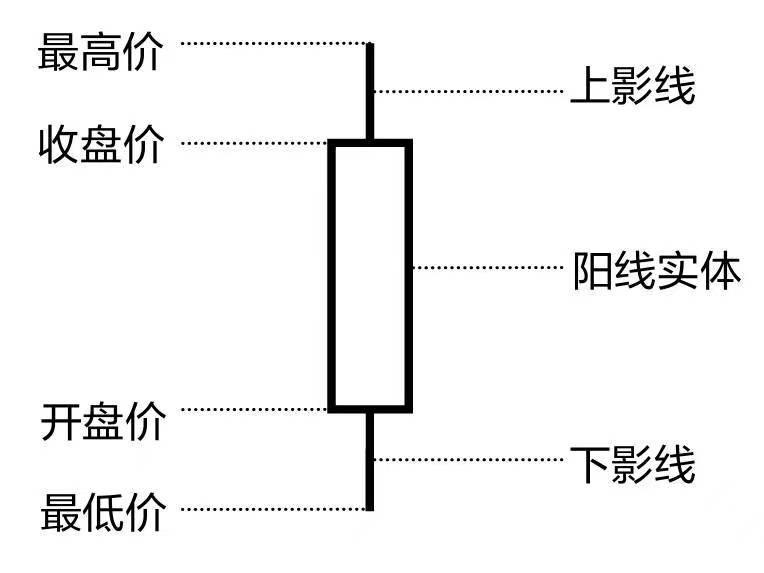
\includegraphics[width=\linewidth ,totalheight=0.95\textheight , keepaspectratio]{K线图阳线.jpg}
\caption{K线图阳线}
\end{figure}

如果当天收盘价低于开盘价,那么就绘制一个阴线实体。上下两条竖线指示的是当天的最低价和最高价。

\begin{figure}[H]
\centering
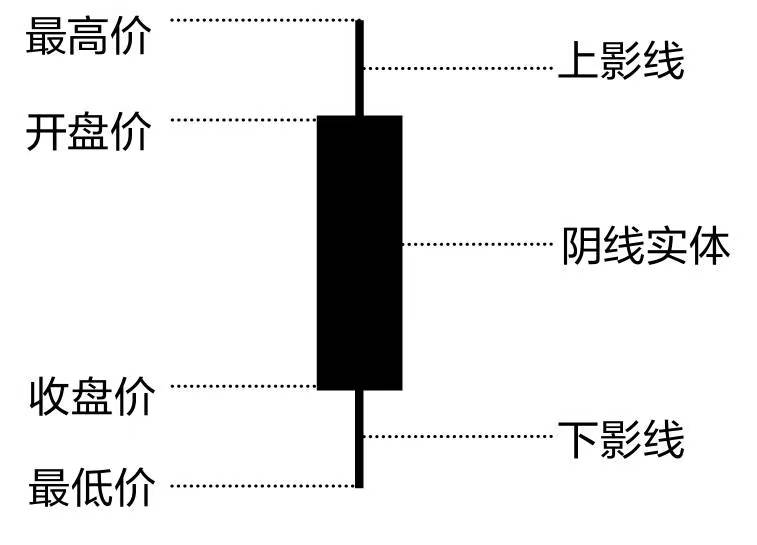
\includegraphics[width=\linewidth ,totalheight=0.95\textheight , keepaspectratio]{K线图阴线.jpg}
\caption{K线图阴线}
\end{figure}


\backmatter
\chapter*{参考资料}
\addchtoc{参考资料}

\begin{thebibliography}{99}
\bibitem[黄帝内经]{黄帝内经} 《黄帝内经》.
\bibitem[好好告别]{好好告别} 《好好告别:世界葬礼观察手记》 by Caitlin Doughty \& 崔倩倩[译] at 2022. 
\bibitem[金融学从入门到精通]{金融学从入门到精通} 《金融学从入门到精通》 by 武永梅 at 2017.
\bibitem[从零开始学K线]{从零开始学K线} 《从零开始学K线》by 唐韩 at 2012. 
\bibitem[聪明的投资者]{聪明的投资者} 《聪明的投资者》by 本杰明·格雷厄姆 \& 贾森·兹威格[评] \& 王中华[译] \& 黄一义[译] at 2016.
\bibitem[轻断食]{轻断食}  《轻断食:正在横扫全球的瘦身革命》 by 麦克尔·莫斯利 \& 咪咪·史宾赛 at 2019.
\bibitem[指数基金投资从入门到精通]{指数基金投资从入门到精通}  《指数基金投资从入门到精通》 by 老罗 at 2018.
\bibitem[疯狂的尿酸]{疯狂的尿酸}  《疯狂的尿酸:不止是痛风》 by 戴维·珀尔马特 \& 王家宁[译] at 2023.
\bibitem[果糖的吸收代谢以及与健康的关系]{果糖的吸收代谢以及与健康的关系}  《果糖的吸收代谢以及与健康的关系》 by 蔡雯雯 \& 李铎 at 2016.
\bibitem[自控力]{自控力}  《自控力》 by [美]麦格尼格尔  \& 王岑卉[译] at 2012.
\bibitem[刻意练习]{刻意练习} 《刻意练习:如何从新手到大师》 by [美]安德斯·艾利克森 \& [美]罗伯特·普尔 \& 王正林[译] at 2016.
\bibitem[圣经的故事]{圣经的故事} 《圣经的故事》 by [美]房龙 \& 朱振武[译] in 上海译文出版社.
\bibitem[新约圣经四福音]{新约圣经四福音} 《新约圣经四福音》by 和合本.
\end{thebibliography}


\end{document}


